\documentclass[twoside]{book}

% Packages required by doxygen
\usepackage{fixltx2e}
\usepackage{calc}
\usepackage{doxygen}
\usepackage[export]{adjustbox} % also loads graphicx
\usepackage{graphicx}
\usepackage[utf8]{inputenc}
\usepackage{makeidx}
\usepackage{multicol}
\usepackage{multirow}
\PassOptionsToPackage{warn}{textcomp}
\usepackage{textcomp}
\usepackage[nointegrals]{wasysym}
\usepackage[table]{xcolor}

% NLS support packages
\usepackage[T2A]{fontenc}
\usepackage[russian]{babel}

% Font selection
\usepackage[T1]{fontenc}
\usepackage[scaled=.90]{helvet}
\usepackage{courier}
\usepackage{amssymb}
\usepackage{sectsty}
\renewcommand{\familydefault}{\sfdefault}
\allsectionsfont{%
  \fontseries{bc}\selectfont%
  \color{darkgray}%
}
\renewcommand{\DoxyLabelFont}{%
  \fontseries{bc}\selectfont%
  \color{darkgray}%
}
\newcommand{\+}{\discretionary{\mbox{\scriptsize$\hookleftarrow$}}{}{}}

% Page & text layout
\usepackage{geometry}
\geometry{%
  a4paper,%
  top=2.5cm,%
  bottom=2.5cm,%
  left=2.5cm,%
  right=2.5cm%
}
\tolerance=750
\hfuzz=15pt
\hbadness=750
\setlength{\emergencystretch}{15pt}
\setlength{\parindent}{0cm}
\setlength{\parskip}{3ex plus 2ex minus 2ex}
\makeatletter
\renewcommand{\paragraph}{%
  \@startsection{paragraph}{4}{0ex}{-1.0ex}{1.0ex}{%
    \normalfont\normalsize\bfseries\SS@parafont%
  }%
}
\renewcommand{\subparagraph}{%
  \@startsection{subparagraph}{5}{0ex}{-1.0ex}{1.0ex}{%
    \normalfont\normalsize\bfseries\SS@subparafont%
  }%
}
\makeatother

% Headers & footers
\usepackage{fancyhdr}
\pagestyle{fancyplain}
\fancyhead[LE]{\fancyplain{}{\bfseries\thepage}}
\fancyhead[CE]{\fancyplain{}{}}
\fancyhead[RE]{\fancyplain{}{\bfseries\leftmark}}
\fancyhead[LO]{\fancyplain{}{\bfseries\rightmark}}
\fancyhead[CO]{\fancyplain{}{}}
\fancyhead[RO]{\fancyplain{}{\bfseries\thepage}}
\fancyfoot[LE]{\fancyplain{}{}}
\fancyfoot[CE]{\fancyplain{}{}}
\fancyfoot[RE]{\fancyplain{}{\bfseries\scriptsize Создано системой Doxygen }}
\fancyfoot[LO]{\fancyplain{}{\bfseries\scriptsize Создано системой Doxygen }}
\fancyfoot[CO]{\fancyplain{}{}}
\fancyfoot[RO]{\fancyplain{}{}}
\renewcommand{\footrulewidth}{0.4pt}
\renewcommand{\chaptermark}[1]{%
  \markboth{#1}{}%
}
\renewcommand{\sectionmark}[1]{%
  \markright{\thesection\ #1}%
}

% Indices & bibliography
\usepackage{natbib}
\usepackage[titles]{tocloft}
\setcounter{tocdepth}{3}
\setcounter{secnumdepth}{5}
\makeindex

% Hyperlinks (required, but should be loaded last)
\usepackage{ifpdf}
\ifpdf
  \usepackage[pdftex,pagebackref=true]{hyperref}
\else
  \usepackage[ps2pdf,pagebackref=true]{hyperref}
\fi
\hypersetup{%
  colorlinks=true,%
  linkcolor=blue,%
  citecolor=blue,%
  unicode%
}

% Custom commands
\newcommand{\clearemptydoublepage}{%
  \newpage{\pagestyle{empty}\cleardoublepage}%
}

\usepackage{caption}
\captionsetup{labelsep=space,justification=centering,font={bf},singlelinecheck=off,skip=4pt,position=top}

%===== C O N T E N T S =====

\begin{document}

% Titlepage & ToC
\hypersetup{pageanchor=false,
             bookmarksnumbered=true,
             pdfencoding=unicode
            }
\pagenumbering{alph}
\begin{titlepage}
\vspace*{7cm}
\begin{center}%
{\Large Optimal Filtering \\[1ex]\large v2.\+7.\+0 }\\
\vspace*{1cm}
{\large Создано системой Doxygen 1.8.12}\\
\end{center}
\end{titlepage}
\clearemptydoublepage
\pagenumbering{roman}
\tableofcontents
\clearemptydoublepage
\pagenumbering{arabic}
\hypersetup{pageanchor=true}

%--- Begin generated contents ---
\chapter{Документация}
\label{index}\hypertarget{index}{}\hypertarget{index_intro_sec}{}\section{Об Optimal Filtering}\label{index_intro_sec}
Основная задача состоит в предоставлении A\+PI для реализации алгоритмов нелинейной фильтрации, их тестирования и сравнения.

Кроме A\+PI имеются готовые реализации нескольких фильтров и задач, на которых они тестируются. Периодически, добавляются новые алгоритмы и задачи.\hypertarget{index_for_compile}{}\section{Что нужно для старта?}\label{index_for_compile}
\hypertarget{index_compilers}{}\subsection{Компиляторы}\label{index_compilers}
Компилятор должен поддерживать стандарт C++11 или более новый. Иначе код не скомпилируется.

Точно скомпилируется (проверено) при использовании \begin{DoxyVerb}  Gсс 4.8 (или новее);

  Clang 5.1 (или новее).
\end{DoxyVerb}


При использоании более старых версий нужно смотреть, поддерживают ли они стандарт C++11.

Другие компиляторы не проверялись.\hypertarget{index_gui}{}\subsection{Графика}\label{index_gui}
Графический интерфейс (G\+UI) написан на Qt. Требуется версия не старше 5.\+0. Рекомендуется Qt 5.\+6.\+1 или новее.

G\+UI -\/ вещь опциональная, вся \char`\"{}математика\char`\"{} написана только с использованием S\+TL и библиотеки Eigen. Так что код можно собрать и вовсе без установленного на машине Qt.\hypertarget{index_qt_bugs}{}\subsection{И ещё...}\label{index_qt_bugs}
Если вы пользуетесь Windows и собираетесь собрать проект с G\+UI не забывайте следующее\+:

Путь к папке с проектом (исходным кодом) не должен содержать кириллицы.

Расположения типа \begin{DoxyVerb}  "C:\Пользователи\...\optimal_filtering2",

  "C:\...\Рабочий стол\...\optimal_filtering2" 
\end{DoxyVerb}


и т.\+д. приведут к невозможности собрать проект -\/ баг Qt на Windows которому 100 лет и, похоже, не будет исправлен никогда =)

Примеры \char`\"{}хорошего\char`\"{} расположения проекта\+: \begin{DoxyVerb}  "C:\Workspace\optimal_filtering2", 

  "D:\optimal_filtering2" \end{DoxyVerb}
 
\chapter{Список задач}
\label{todo}
\hypertarget{todo}{}

\begin{DoxyRefList}
\item[\label{todo__todo000001}%
\hypertarget{todo__todo000001}{}%
Член \hyperlink{class_graph_window_a51f89adcbef5b90b9fdbb24bf7536fe5}{Graph\+Window\+:\+:on\+Save\+Png} ()]Расширение \char`\"{}.\+png\char`\"{} не добавляется к концу имени файла автоматически. Надо запилить. 
\end{DoxyRefList}
\chapter{Алфавитный указатель пространств имен}
\section{Пространства имен}
Полный список документированных пространств имен.\begin{DoxyCompactList}
\item\contentsline{section}{\hyperlink{namespace_core}{Core} \\*Модуль, содержащий основные классы и методы }{\pageref{namespace_core}}{}
\item\contentsline{section}{\hyperlink{namespace_filters}{Filters} \\*Модуль, содержащий реализации конкретных алгоритмов фильтрации }{\pageref{namespace_filters}}{}
\item\contentsline{section}{\hyperlink{namespace_filters_1_1_continuous}{Filters\+::\+Continuous} \\*Подмодуль, содержащий реализации непрерывных фильтров оптимальной структуры }{\pageref{namespace_filters_1_1_continuous}}{}
\item\contentsline{section}{\hyperlink{namespace_filters_1_1_continuous_discrete}{Filters\+::\+Continuous\+Discrete} \\*Подмодуль, содержащий реализации непрерывно-\/дискретных фильтров оптимальной структуры }{\pageref{namespace_filters_1_1_continuous_discrete}}{}
\item\contentsline{section}{\hyperlink{namespace_filters_1_1_discrete}{Filters\+::\+Discrete} \\*Подмодуль, содержащий реализации дискретных фильтров оптимальной структуры }{\pageref{namespace_filters_1_1_discrete}}{}
\item\contentsline{section}{\hyperlink{namespace_math}{Math} \\*Модуль, содержащий описание и реализацию задач математических методов и типов }{\pageref{namespace_math}}{}
\item\contentsline{section}{\hyperlink{namespace_math_1_1_convert}{Math\+::\+Convert} \\*Модуль, содержащий описание и реализацию методов конвертирования значений между системами }{\pageref{namespace_math_1_1_convert}}{}
\item\contentsline{section}{\hyperlink{namespace_math_1_1_lin_alg}{Math\+::\+Lin\+Alg} \\*Модуль, содержащий описание и реализацию методов линейной алгебры }{\pageref{namespace_math_1_1_lin_alg}}{}
\item\contentsline{section}{\hyperlink{namespace_math_1_1_rand}{Math\+::\+Rand} \\*Модуль, содержащий описание и реализацию методов генерации случайных величин }{\pageref{namespace_math_1_1_rand}}{}
\item\contentsline{section}{\hyperlink{namespace_math_1_1_statistic}{Math\+::\+Statistic} \\*Модуль, содержащий описание и реализацию методов работы с моментными характеристиками СВ }{\pageref{namespace_math_1_1_statistic}}{}
\item\contentsline{section}{\hyperlink{namespace_tasks}{Tasks} \\*Модуль, содержащий реализации конкретных задач для фильтров }{\pageref{namespace_tasks}}{}
\item\contentsline{section}{\hyperlink{namespace_tasks_1_1_continuous}{Tasks\+::\+Continuous} \\*Подмодуль, содержащий реализации задач для непрерывных фильтров оптимальной структуры }{\pageref{namespace_tasks_1_1_continuous}}{}
\item\contentsline{section}{\hyperlink{namespace_tasks_1_1_continuous_discrete}{Tasks\+::\+Continuous\+Discrete} \\*Подмодуль, содержащий реализации задач для непрерывно-\/дискретных фильтров оптимальной структуры }{\pageref{namespace_tasks_1_1_continuous_discrete}}{}
\item\contentsline{section}{\hyperlink{namespace_tasks_1_1_discrete}{Tasks\+::\+Discrete} \\*Подмодуль, содержащий реализации задач для дискретных фильтров оптимальной структуры }{\pageref{namespace_tasks_1_1_discrete}}{}
\end{DoxyCompactList}

\chapter{Иерархический список классов}
\section{Иерархия классов}
Иерархия классов.\begin{DoxyCompactList}
\item \contentsline{section}{Color\+Manager}{\pageref{class_color_manager}}{}
\item \contentsline{section}{Math\+:\+:Const}{\pageref{class_math_1_1_const}}{}
\item \contentsline{section}{Core\+:\+:Filter}{\pageref{class_core_1_1_filter}}{}
\begin{DoxyCompactList}
\item \contentsline{section}{Core\+:\+:Continuous\+Discrete\+Filter}{\pageref{class_core_1_1_continuous_discrete_filter}}{}
\begin{DoxyCompactList}
\item \contentsline{section}{Filters\+:\+:Continuous\+Discrete\+:\+:A\+OF}{\pageref{class_filters_1_1_continuous_discrete_1_1_a_o_f}}{}
\item \contentsline{section}{Filters\+:\+:Continuous\+Discrete\+:\+:D\+F\+OS}{\pageref{class_filters_1_1_continuous_discrete_1_1_d_f_o_s}}{}
\item \contentsline{section}{Filters\+:\+:Continuous\+Discrete\+:\+:D\+F\+O\+S\+BO}{\pageref{class_filters_1_1_continuous_discrete_1_1_d_f_o_s_b_o}}{}
\item \contentsline{section}{Filters\+:\+:Continuous\+Discrete\+:\+:F\+OS}{\pageref{class_filters_1_1_continuous_discrete_1_1_f_o_s}}{}
\end{DoxyCompactList}
\item \contentsline{section}{Core\+:\+:Continuous\+Filter}{\pageref{class_core_1_1_continuous_filter}}{}
\begin{DoxyCompactList}
\item \contentsline{section}{Filters\+:\+:Continuous\+:\+:A\+OF}{\pageref{class_filters_1_1_continuous_1_1_a_o_f}}{}
\item \contentsline{section}{Filters\+:\+:Continuous\+:\+:F\+OS}{\pageref{class_filters_1_1_continuous_1_1_f_o_s}}{}
\end{DoxyCompactList}
\item \contentsline{section}{Core\+:\+:Discrete\+Filter}{\pageref{class_core_1_1_discrete_filter}}{}
\begin{DoxyCompactList}
\item \contentsline{section}{Filters\+:\+:Discrete\+:\+:A\+OF}{\pageref{class_filters_1_1_discrete_1_1_a_o_f}}{}
\item \contentsline{section}{Filters\+:\+:Discrete\+:\+:F\+OS}{\pageref{class_filters_1_1_discrete_1_1_f_o_s}}{}
\item \contentsline{section}{Filters\+:\+:Discrete\+:\+:M\+F\+OS}{\pageref{class_filters_1_1_discrete_1_1_m_f_o_s}}{}
\end{DoxyCompactList}
\end{DoxyCompactList}
\item \contentsline{section}{Filters\+:\+:Filter\+Factory}{\pageref{class_filters_1_1_filter_factory}}{}
\item \contentsline{section}{Core\+:\+:Filter\+Parameters}{\pageref{class_core_1_1_filter_parameters}}{}
\item \contentsline{section}{Font\+Manager}{\pageref{class_font_manager}}{}
\item \contentsline{section}{Core\+:\+:Function\+Time}{\pageref{class_core_1_1_function_time}}{}
\begin{DoxyCompactList}
\item \contentsline{section}{Core\+:\+:Task}{\pageref{class_core_1_1_task}}{}
\begin{DoxyCompactList}
\item \contentsline{section}{Core\+:\+:Continuous\+Discrete\+Task}{\pageref{class_core_1_1_continuous_discrete_task}}{}
\begin{DoxyCompactList}
\item \contentsline{section}{Tasks\+:\+:Continuous\+Discrete\+:\+:Landing\+Linear}{\pageref{class_tasks_1_1_continuous_discrete_1_1_landing_linear}}{}
\begin{DoxyCompactList}
\item \contentsline{section}{Tasks\+:\+:Continuous\+Discrete\+:\+:Landing\+Gauss}{\pageref{class_tasks_1_1_continuous_discrete_1_1_landing_gauss}}{}
\end{DoxyCompactList}
\item \contentsline{section}{Tasks\+:\+:Continuous\+Discrete\+:\+:Van\+Der\+Pol\+Linear}{\pageref{class_tasks_1_1_continuous_discrete_1_1_van_der_pol_linear}}{}
\begin{DoxyCompactList}
\item \contentsline{section}{Tasks\+:\+:Continuous\+Discrete\+:\+:Van\+Der\+Pol\+Gauss}{\pageref{class_tasks_1_1_continuous_discrete_1_1_van_der_pol_gauss}}{}
\end{DoxyCompactList}
\end{DoxyCompactList}
\item \contentsline{section}{Core\+:\+:Continuous\+Task}{\pageref{class_core_1_1_continuous_task}}{}
\begin{DoxyCompactList}
\item \contentsline{section}{Tasks\+:\+:Continuous\+:\+:Landing\+Linear}{\pageref{class_tasks_1_1_continuous_1_1_landing_linear}}{}
\begin{DoxyCompactList}
\item \contentsline{section}{Tasks\+:\+:Continuous\+:\+:Landing\+Gauss}{\pageref{class_tasks_1_1_continuous_1_1_landing_gauss}}{}
\end{DoxyCompactList}
\item \contentsline{section}{Tasks\+:\+:Continuous\+:\+:Van\+Der\+Pol\+Linear}{\pageref{class_tasks_1_1_continuous_1_1_van_der_pol_linear}}{}
\begin{DoxyCompactList}
\item \contentsline{section}{Tasks\+:\+:Continuous\+:\+:Van\+Der\+Pol\+Gauss}{\pageref{class_tasks_1_1_continuous_1_1_van_der_pol_gauss}}{}
\end{DoxyCompactList}
\end{DoxyCompactList}
\item \contentsline{section}{Core\+:\+:Discrete\+Task}{\pageref{class_core_1_1_discrete_task}}{}
\begin{DoxyCompactList}
\item \contentsline{section}{Tasks\+:\+:Discrete\+:\+:Landing\+Linear}{\pageref{class_tasks_1_1_discrete_1_1_landing_linear}}{}
\begin{DoxyCompactList}
\item \contentsline{section}{Tasks\+:\+:Discrete\+:\+:Landing\+Gauss}{\pageref{class_tasks_1_1_discrete_1_1_landing_gauss}}{}
\end{DoxyCompactList}
\end{DoxyCompactList}
\end{DoxyCompactList}
\end{DoxyCompactList}
\item \contentsline{section}{G\+Axis\+Range}{\pageref{struct_g_axis_range}}{}
\item \contentsline{section}{G\+Curve}{\pageref{struct_g_curve}}{}
\item \contentsline{section}{Graph\+Sheet}{\pageref{class_graph_sheet}}{}
\item \contentsline{section}{Core\+:\+:Info}{\pageref{class_core_1_1_info}}{}
\item Q\+Dialog\begin{DoxyCompactList}
\item \contentsline{section}{Ranges\+Dialog}{\pageref{class_ranges_dialog}}{}
\end{DoxyCompactList}
\item Q\+Group\+Box\begin{DoxyCompactList}
\item \contentsline{section}{Additional\+Settings\+Widget}{\pageref{class_additional_settings_widget}}{}
\item \contentsline{section}{Filter\+Parameters\+Widget}{\pageref{class_filter_parameters_widget}}{}
\item \contentsline{section}{Filter\+Start\+Buttons\+Box}{\pageref{class_filter_start_buttons_box}}{}
\item \contentsline{section}{Task\+Widget}{\pageref{class_task_widget}}{}
\end{DoxyCompactList}
\item Q\+Main\+Window\begin{DoxyCompactList}
\item \contentsline{section}{Filter\+Results\+Table}{\pageref{class_filter_results_table}}{}
\item \contentsline{section}{Graph\+Window}{\pageref{class_graph_window}}{}
\item \contentsline{section}{Main\+Window}{\pageref{class_main_window}}{}
\end{DoxyCompactList}
\item Q\+Widget\begin{DoxyCompactList}
\item \contentsline{section}{Matrix\+Widget}{\pageref{class_matrix_widget}}{}
\item \contentsline{section}{Task\+Parameters\+Widget}{\pageref{class_task_parameters_widget}}{}
\end{DoxyCompactList}
\item \contentsline{section}{Core\+:\+:Single\+Filter\+Output}{\pageref{struct_core_1_1_single_filter_output}}{}
\item \contentsline{section}{Tasks\+:\+:Task\+Factory}{\pageref{class_tasks_1_1_task_factory}}{}
\end{DoxyCompactList}

\chapter{Алфавитный указатель классов}
\section{Классы}
Классы с их кратким описанием.\begin{DoxyCompactList}
\item\contentsline{section}{\hyperlink{class_additional_settings_widget}{Additional\+Settings\+Widget} \\*Класс виджета, предаставляющего дополнительные настройки для численных методов }{\pageref{class_additional_settings_widget}}{}
\item\contentsline{section}{\hyperlink{class_filters_1_1_continuous_1_1_a_o_f}{Filters\+::\+Continuous\+::\+A\+OF} \\*Класс, реализующий непрерывный абсолютно оптимальный фильтр }{\pageref{class_filters_1_1_continuous_1_1_a_o_f}}{}
\item\contentsline{section}{\hyperlink{class_filters_1_1_continuous_discrete_1_1_a_o_f}{Filters\+::\+Continuous\+Discrete\+::\+A\+OF} \\*Класс, реализующий непрерывно-\/дискретный абсолютно оптимальной фильтр }{\pageref{class_filters_1_1_continuous_discrete_1_1_a_o_f}}{}
\item\contentsline{section}{\hyperlink{class_filters_1_1_discrete_1_1_a_o_f}{Filters\+::\+Discrete\+::\+A\+OF} \\*Класс, реализующий дискретный абсолютно оптимальной фильтр }{\pageref{class_filters_1_1_discrete_1_1_a_o_f}}{}
\item\contentsline{section}{\hyperlink{class_color_manager}{Color\+Manager} \\*Класс для управления набором цветов }{\pageref{class_color_manager}}{}
\item\contentsline{section}{\hyperlink{class_math_1_1_const}{Math\+::\+Const} \\*Статический класс, содержащий константы }{\pageref{class_math_1_1_const}}{}
\item\contentsline{section}{\hyperlink{class_core_1_1_continuous_discrete_filter}{Core\+::\+Continuous\+Discrete\+Filter} \\*Базовый класс для всех непрерывно-\/дискретных фильтров оптимальной структуры }{\pageref{class_core_1_1_continuous_discrete_filter}}{}
\item\contentsline{section}{\hyperlink{class_core_1_1_continuous_discrete_task}{Core\+::\+Continuous\+Discrete\+Task} \\*Базовый тип задач для непрерывно-\/дискретных фильтров оптимальной структуры }{\pageref{class_core_1_1_continuous_discrete_task}}{}
\item\contentsline{section}{\hyperlink{class_core_1_1_continuous_filter}{Core\+::\+Continuous\+Filter} \\*Базовый класс для всех непрерывныз фильтров оптимальной структуры }{\pageref{class_core_1_1_continuous_filter}}{}
\item\contentsline{section}{\hyperlink{class_core_1_1_continuous_task}{Core\+::\+Continuous\+Task} \\*Базовый тип задач для непрерывных фильтров оптимальной структуры }{\pageref{class_core_1_1_continuous_task}}{}
\item\contentsline{section}{\hyperlink{class_math_1_1_lin_alg_1_1_current_pinv_method}{Math\+::\+Lin\+Alg\+::\+Current\+Pinv\+Method} \\*Класс, упрощающий выбор метода псевдообращения матриц }{\pageref{class_math_1_1_lin_alg_1_1_current_pinv_method}}{}
\item\contentsline{section}{\hyperlink{class_filters_1_1_continuous_discrete_1_1_d_f_o_s}{Filters\+::\+Continuous\+Discrete\+::\+D\+F\+OS} \\*Класс, реализующий непрерывно-\/дискретный фильтр оптимальной структуры с дискретным прогнозом }{\pageref{class_filters_1_1_continuous_discrete_1_1_d_f_o_s}}{}
\item\contentsline{section}{\hyperlink{class_filters_1_1_continuous_discrete_1_1_d_f_o_s_b_o}{Filters\+::\+Continuous\+Discrete\+::\+D\+F\+O\+S\+BO} \\*Класс, реализующий непрерывно-\/дискретный фильтр оптимальной структуры повышеного порядка }{\pageref{class_filters_1_1_continuous_discrete_1_1_d_f_o_s_b_o}}{}
\item\contentsline{section}{\hyperlink{class_core_1_1_discrete_filter}{Core\+::\+Discrete\+Filter} \\*Базовый класс для всех дискретных фильтров оптимальной структуры }{\pageref{class_core_1_1_discrete_filter}}{}
\item\contentsline{section}{\hyperlink{class_core_1_1_discrete_task}{Core\+::\+Discrete\+Task} \\*Базовый тип задач для дискретных фильтров оптимальной структуры }{\pageref{class_core_1_1_discrete_task}}{}
\item\contentsline{section}{\hyperlink{class_core_1_1_filter}{Core\+::\+Filter} \\*Базовый класс для всех фильтров }{\pageref{class_core_1_1_filter}}{}
\item\contentsline{section}{\hyperlink{class_filters_1_1_filter_factory}{Filters\+::\+Filter\+Factory} \\*Фабричный класс для создания экземпляров классов фильтров }{\pageref{class_filters_1_1_filter_factory}}{}
\item\contentsline{section}{\hyperlink{class_core_1_1_filter_parameters}{Core\+::\+Filter\+Parameters} \\*Класс для работы с параметрами фильтра }{\pageref{class_core_1_1_filter_parameters}}{}
\item\contentsline{section}{\hyperlink{class_filter_parameters_widget}{Filter\+Parameters\+Widget} \\*Класс виджета, предаставляющего элементы управления параметрами фильтрации }{\pageref{class_filter_parameters_widget}}{}
\item\contentsline{section}{\hyperlink{class_filter_results_table}{Filter\+Results\+Table} \\*Виджет для отображения таблиц }{\pageref{class_filter_results_table}}{}
\item\contentsline{section}{\hyperlink{class_filter_start_buttons_box}{Filter\+Start\+Buttons\+Box} \\*Класс виджета, содержащего только кнопки для запуска того или иного фильтра }{\pageref{class_filter_start_buttons_box}}{}
\item\contentsline{section}{\hyperlink{class_font_manager}{Font\+Manager} \\*Статический класс для работы с загружаемыми из файлов шрифтами (singleton) }{\pageref{class_font_manager}}{}
\item\contentsline{section}{\hyperlink{class_filters_1_1_continuous_1_1_f_o_s}{Filters\+::\+Continuous\+::\+F\+OS} \\*Класс, реализующий непрерывный фильтр оптимальной структуры }{\pageref{class_filters_1_1_continuous_1_1_f_o_s}}{}
\item\contentsline{section}{\hyperlink{class_filters_1_1_continuous_discrete_1_1_f_o_s}{Filters\+::\+Continuous\+Discrete\+::\+F\+OS} \\*Класс, реализующий непрерывно-\/дискретный фильтр оптимальной структуры с непрерывным прогнозом }{\pageref{class_filters_1_1_continuous_discrete_1_1_f_o_s}}{}
\item\contentsline{section}{\hyperlink{class_filters_1_1_discrete_1_1_f_o_s}{Filters\+::\+Discrete\+::\+F\+OS} \\*Класс, реализующий дискретный фильтр оптимальной структуры }{\pageref{class_filters_1_1_discrete_1_1_f_o_s}}{}
\item\contentsline{section}{\hyperlink{class_core_1_1_function_time}{Core\+::\+Function\+Time} \\*Базовый класс для классов, представляющих собой функции времени }{\pageref{class_core_1_1_function_time}}{}
\item\contentsline{section}{\hyperlink{struct_g_axis_range}{G\+Axis\+Range} \\*Структура для хранения границ осей координат }{\pageref{struct_g_axis_range}}{}
\item\contentsline{section}{\hyperlink{struct_g_curve}{G\+Curve} \\*Структура для хранения кривой }{\pageref{struct_g_curve}}{}
\item\contentsline{section}{\hyperlink{class_graph_sheet}{Graph\+Sheet} \\*Класс, реализующий \char`\"{}страницу\char`\"{} окна графиков }{\pageref{class_graph_sheet}}{}
\item\contentsline{section}{\hyperlink{class_graph_window}{Graph\+Window} \\*Класс, реализующий окно для просмотра графиков }{\pageref{class_graph_window}}{}
\item\contentsline{section}{\hyperlink{class_core_1_1_info}{Core\+::\+Info} \\*Класс для хранения строковой информации о чем-\/либо }{\pageref{class_core_1_1_info}}{}
\item\contentsline{section}{\hyperlink{class_tasks_1_1_continuous_1_1_landing_gauss}{Tasks\+::\+Continuous\+::\+Landing\+Gauss} }{\pageref{class_tasks_1_1_continuous_1_1_landing_gauss}}{}
\item\contentsline{section}{\hyperlink{class_tasks_1_1_continuous_discrete_1_1_landing_gauss}{Tasks\+::\+Continuous\+Discrete\+::\+Landing\+Gauss} }{\pageref{class_tasks_1_1_continuous_discrete_1_1_landing_gauss}}{}
\item\contentsline{section}{\hyperlink{class_tasks_1_1_discrete_1_1_landing_gauss}{Tasks\+::\+Discrete\+::\+Landing\+Gauss} }{\pageref{class_tasks_1_1_discrete_1_1_landing_gauss}}{}
\item\contentsline{section}{\hyperlink{class_tasks_1_1_continuous_1_1_landing_linear}{Tasks\+::\+Continuous\+::\+Landing\+Linear} \\*Задача спуска ЛА на планету (непрерывная, линеаризованная) для фильтров оптимальной структуры }{\pageref{class_tasks_1_1_continuous_1_1_landing_linear}}{}
\item\contentsline{section}{\hyperlink{class_tasks_1_1_discrete_1_1_landing_linear}{Tasks\+::\+Discrete\+::\+Landing\+Linear} \\*Задача спуска ЛА на планету (дискретная, линеаризованная) для фильтров оптимальной структуры }{\pageref{class_tasks_1_1_discrete_1_1_landing_linear}}{}
\item\contentsline{section}{\hyperlink{class_tasks_1_1_continuous_discrete_1_1_landing_linear}{Tasks\+::\+Continuous\+Discrete\+::\+Landing\+Linear} \\*Задача спуска ЛА на планету (непрерывно-\/дискретная, линеаризованная) для фильтров оптимальной структуры }{\pageref{class_tasks_1_1_continuous_discrete_1_1_landing_linear}}{}
\item\contentsline{section}{\hyperlink{class_main_window}{Main\+Window} \\*Класс для главного окна приложения }{\pageref{class_main_window}}{}
\item\contentsline{section}{\hyperlink{class_matrix_widget}{Matrix\+Widget} \\*Класс для отображения / изменения матриц (или векторов) }{\pageref{class_matrix_widget}}{}
\item\contentsline{section}{\hyperlink{class_filters_1_1_discrete_1_1_m_f_o_s}{Filters\+::\+Discrete\+::\+M\+F\+OS} }{\pageref{class_filters_1_1_discrete_1_1_m_f_o_s}}{}
\item\contentsline{section}{\hyperlink{class_math_1_1_multivariate_normal_distribution}{Math\+::\+Multivariate\+Normal\+Distribution} \\*Класс-\/генератор случайных нормальных(гауссовских) векторов }{\pageref{class_math_1_1_multivariate_normal_distribution}}{}
\item\contentsline{section}{\hyperlink{class_math_1_1_random_properties}{Math\+::\+Random\+Properties} \\*Статический класс, помогающий управлять генератором ПСЧ }{\pageref{class_math_1_1_random_properties}}{}
\item\contentsline{section}{\hyperlink{class_ranges_dialog}{Ranges\+Dialog} \\*Диалоговое окно для изменения границ осей координат }{\pageref{class_ranges_dialog}}{}
\item\contentsline{section}{\hyperlink{struct_core_1_1_single_filter_output}{Core\+::\+Single\+Filter\+Output} \\*Структура, хранящая значение времени и моментные характеристики, соответствующие ему }{\pageref{struct_core_1_1_single_filter_output}}{}
\item\contentsline{section}{\hyperlink{class_core_1_1_task}{Core\+::\+Task} \\*Базовый класс для всех задач }{\pageref{class_core_1_1_task}}{}
\item\contentsline{section}{\hyperlink{class_tasks_1_1_task_factory}{Tasks\+::\+Task\+Factory} \\*Фабричный класс для создания экземпляров классов задач }{\pageref{class_tasks_1_1_task_factory}}{}
\item\contentsline{section}{\hyperlink{class_task_parameters_widget}{Task\+Parameters\+Widget} \\*Класс виджета, предаставляющего возможность работы с параметрами задач }{\pageref{class_task_parameters_widget}}{}
\item\contentsline{section}{\hyperlink{class_task_widget}{Task\+Widget} \\*Виджет для работы с задачами для фильтров }{\pageref{class_task_widget}}{}
\item\contentsline{section}{\hyperlink{class_tasks_1_1_continuous_discrete_1_1_van_der_pol_gauss}{Tasks\+::\+Continuous\+Discrete\+::\+Van\+Der\+Pol\+Gauss} \\*Осциллятор Ван-\/дер-\/Поля (непрерывно-\/дискретный, гауссовский) для фильтров оптимальной структуры }{\pageref{class_tasks_1_1_continuous_discrete_1_1_van_der_pol_gauss}}{}
\item\contentsline{section}{\hyperlink{class_tasks_1_1_continuous_1_1_van_der_pol_gauss}{Tasks\+::\+Continuous\+::\+Van\+Der\+Pol\+Gauss} \\*Осциллятор Ван-\/дер-\/Поля (непрерывный, гауссовский) для фильтров оптимальной структуры }{\pageref{class_tasks_1_1_continuous_1_1_van_der_pol_gauss}}{}
\item\contentsline{section}{\hyperlink{class_tasks_1_1_continuous_1_1_van_der_pol_linear}{Tasks\+::\+Continuous\+::\+Van\+Der\+Pol\+Linear} \\*Осциллятор Ван-\/дер-\/Поля (непрерывный, линеаризованный) для фильтров оптимальной структуры }{\pageref{class_tasks_1_1_continuous_1_1_van_der_pol_linear}}{}
\item\contentsline{section}{\hyperlink{class_tasks_1_1_continuous_discrete_1_1_van_der_pol_linear}{Tasks\+::\+Continuous\+Discrete\+::\+Van\+Der\+Pol\+Linear} \\*Осциллятор Ван-\/дер-\/Поля (непрерывно-\/дискретный, линеаризованный) для фильтров оптимальной структуры }{\pageref{class_tasks_1_1_continuous_discrete_1_1_van_der_pol_linear}}{}
\end{DoxyCompactList}

\chapter{Пространства имен}
\hypertarget{namespace_core}{}\section{Пространство имен Core}
\label{namespace_core}\index{Core@{Core}}


Модуль, содержащий основные классы и методы.  


\subsection*{Классы}
\begin{DoxyCompactItemize}
\item 
class \hyperlink{class_core_1_1_continuous_discrete_filter}{Continuous\+Discrete\+Filter}
\begin{DoxyCompactList}\small\item\em Базовый класс для всех непрерывно-\/дискретных фильтров оптимальной структуры. \end{DoxyCompactList}\item 
class \hyperlink{class_core_1_1_continuous_discrete_task}{Continuous\+Discrete\+Task}
\begin{DoxyCompactList}\small\item\em Базовый тип задач для непрерывно-\/дискретных фильтров оптимальной структуры. \end{DoxyCompactList}\item 
class \hyperlink{class_core_1_1_continuous_filter}{Continuous\+Filter}
\begin{DoxyCompactList}\small\item\em Базовый класс для всех непрерывныз фильтров оптимальной структуры. \end{DoxyCompactList}\item 
class \hyperlink{class_core_1_1_continuous_task}{Continuous\+Task}
\begin{DoxyCompactList}\small\item\em Базовый тип задач для непрерывных фильтров оптимальной структуры. \end{DoxyCompactList}\item 
class \hyperlink{class_core_1_1_discrete_filter}{Discrete\+Filter}
\begin{DoxyCompactList}\small\item\em Базовый класс для всех дискретных фильтров оптимальной структуры. \end{DoxyCompactList}\item 
class \hyperlink{class_core_1_1_discrete_task}{Discrete\+Task}
\begin{DoxyCompactList}\small\item\em Базовый тип задач для дискретных фильтров оптимальной структуры. \end{DoxyCompactList}\item 
class \hyperlink{class_core_1_1_filter}{Filter}
\begin{DoxyCompactList}\small\item\em Базовый класс для всех фильтров. \end{DoxyCompactList}\item 
class \hyperlink{class_core_1_1_filter_parameters}{Filter\+Parameters}
\begin{DoxyCompactList}\small\item\em Класс для работы с параметрами фильтра. \end{DoxyCompactList}\item 
class \hyperlink{class_core_1_1_function_time}{Function\+Time}
\begin{DoxyCompactList}\small\item\em Базовый класс для классов, представляющих собой функции времени. \end{DoxyCompactList}\item 
class \hyperlink{class_core_1_1_info}{Info}
\begin{DoxyCompactList}\small\item\em Класс для хранения строковой информации о чем-\/либо. \end{DoxyCompactList}\item 
struct \hyperlink{struct_core_1_1_single_filter_output}{Single\+Filter\+Output}
\begin{DoxyCompactList}\small\item\em Структура, хранящая значение времени и моментные характеристики, соответствующие ему. \end{DoxyCompactList}\item 
class \hyperlink{class_core_1_1_task}{Task}
\begin{DoxyCompactList}\small\item\em Базовый класс для всех задач \end{DoxyCompactList}\end{DoxyCompactItemize}
\subsection*{Определения типов}
\begin{DoxyCompactItemize}
\item 
using \hyperlink{namespace_core_a70dec7db05bb1e9e8d105d188633fe91}{Ptr\+C\+D\+Filter} = std\+::shared\+\_\+ptr$<$ \hyperlink{class_core_1_1_continuous_discrete_filter}{Continuous\+Discrete\+Filter} $>$\hypertarget{namespace_core_a70dec7db05bb1e9e8d105d188633fe91}{}\label{namespace_core_a70dec7db05bb1e9e8d105d188633fe91}

\begin{DoxyCompactList}\small\item\em Тип умного указателя на \hyperlink{class_core_1_1_continuous_discrete_filter}{Continuous\+Discrete\+Filter}. \end{DoxyCompactList}\item 
using \hyperlink{namespace_core_a4d5939b0284102299f3fb63d7552826a}{Ptr\+C\+D\+Task} = std\+::shared\+\_\+ptr$<$ \hyperlink{class_core_1_1_continuous_discrete_task}{Continuous\+Discrete\+Task} $>$\hypertarget{namespace_core_a4d5939b0284102299f3fb63d7552826a}{}\label{namespace_core_a4d5939b0284102299f3fb63d7552826a}

\begin{DoxyCompactList}\small\item\em Тип умного указателя на \hyperlink{class_core_1_1_continuous_discrete_task}{Continuous\+Discrete\+Task}. \end{DoxyCompactList}\item 
using \hyperlink{namespace_core_a83a912e3fc57bd838d6ddc39895999f3}{Ptr\+C\+Filter} = std\+::shared\+\_\+ptr$<$ \hyperlink{class_core_1_1_continuous_filter}{Continuous\+Filter} $>$\hypertarget{namespace_core_a83a912e3fc57bd838d6ddc39895999f3}{}\label{namespace_core_a83a912e3fc57bd838d6ddc39895999f3}

\begin{DoxyCompactList}\small\item\em Тип умного указателя на \hyperlink{class_core_1_1_continuous_filter}{Continuous\+Filter}. \end{DoxyCompactList}\item 
using \hyperlink{namespace_core_a95543587a560c6c497c6cadf68e03a62}{Ptr\+C\+Task} = std\+::shared\+\_\+ptr$<$ \hyperlink{class_core_1_1_continuous_task}{Continuous\+Task} $>$\hypertarget{namespace_core_a95543587a560c6c497c6cadf68e03a62}{}\label{namespace_core_a95543587a560c6c497c6cadf68e03a62}

\begin{DoxyCompactList}\small\item\em Тип умного указателя на \hyperlink{class_core_1_1_continuous_task}{Continuous\+Task}. \end{DoxyCompactList}\item 
using \hyperlink{namespace_core_a5bc2ef0a7d6facf16009f89297174aa6}{Ptr\+D\+Filter} = std\+::shared\+\_\+ptr$<$ \hyperlink{class_core_1_1_discrete_filter}{Discrete\+Filter} $>$\hypertarget{namespace_core_a5bc2ef0a7d6facf16009f89297174aa6}{}\label{namespace_core_a5bc2ef0a7d6facf16009f89297174aa6}

\begin{DoxyCompactList}\small\item\em Тип умного указателя на \hyperlink{class_core_1_1_discrete_filter}{Discrete\+Filter}. \end{DoxyCompactList}\item 
using \hyperlink{namespace_core_a9cd3f9b81303651b8d115031018f0ebf}{Ptr\+D\+Task} = std\+::shared\+\_\+ptr$<$ \hyperlink{class_core_1_1_discrete_task}{Discrete\+Task} $>$\hypertarget{namespace_core_a9cd3f9b81303651b8d115031018f0ebf}{}\label{namespace_core_a9cd3f9b81303651b8d115031018f0ebf}

\begin{DoxyCompactList}\small\item\em Тип умного указателя на \hyperlink{class_core_1_1_discrete_task}{Discrete\+Task}. \end{DoxyCompactList}\item 
using \hyperlink{namespace_core_afba80c2cb714c7d5793d9bcb9591e156}{Ptr\+Filter} = std\+::shared\+\_\+ptr$<$ \hyperlink{class_core_1_1_filter}{Filter} $>$\hypertarget{namespace_core_afba80c2cb714c7d5793d9bcb9591e156}{}\label{namespace_core_afba80c2cb714c7d5793d9bcb9591e156}

\begin{DoxyCompactList}\small\item\em Тип умного указателя на \hyperlink{class_core_1_1_filter}{Filter}. \end{DoxyCompactList}\item 
using \hyperlink{namespace_core_a60877581a235fc9566087b54d463ce9c}{Filter\+Output} = Array$<$ \hyperlink{struct_core_1_1_single_filter_output}{Single\+Filter\+Output} $>$\hypertarget{namespace_core_a60877581a235fc9566087b54d463ce9c}{}\label{namespace_core_a60877581a235fc9566087b54d463ce9c}

\begin{DoxyCompactList}\small\item\em Тип результата работы фильтра. \end{DoxyCompactList}\item 
using {\bfseries Array\+Dbl} = Array$<$ double $>$\hypertarget{namespace_core_afad0f3873edb3dbb0f2f845357db225d}{}\label{namespace_core_afad0f3873edb3dbb0f2f845357db225d}

\item 
using \hyperlink{namespace_core_a4811af8148ba137d644b9a61a042cf03}{Ptr\+Filter\+Parameters} = std\+::shared\+\_\+ptr$<$ \hyperlink{class_core_1_1_filter_parameters}{Filter\+Parameters} $>$\hypertarget{namespace_core_a4811af8148ba137d644b9a61a042cf03}{}\label{namespace_core_a4811af8148ba137d644b9a61a042cf03}

\begin{DoxyCompactList}\small\item\em Тип умного указателя на \hyperlink{class_core_1_1_filter_parameters}{Filter\+Parameters}. \end{DoxyCompactList}\item 
using \hyperlink{namespace_core_a647483da8a1266d5bbd3e9bb5cd66d08}{Ptr\+Info} = std\+::shared\+\_\+ptr$<$ \hyperlink{class_core_1_1_info}{Info} $>$\hypertarget{namespace_core_a647483da8a1266d5bbd3e9bb5cd66d08}{}\label{namespace_core_a647483da8a1266d5bbd3e9bb5cd66d08}

\begin{DoxyCompactList}\small\item\em Тип умного указателя на \hyperlink{class_core_1_1_info}{Info}. \end{DoxyCompactList}\item 
using \hyperlink{namespace_core_a34db09964ddb6b4af04cc94b02a49e29}{Task\+Parameters} = std\+::map$<$ std\+::string, double $>$\hypertarget{namespace_core_a34db09964ddb6b4af04cc94b02a49e29}{}\label{namespace_core_a34db09964ddb6b4af04cc94b02a49e29}

\begin{DoxyCompactList}\small\item\em Тип параметров задачи. \end{DoxyCompactList}\item 
using \hyperlink{namespace_core_a3e0e555656bf795146ebb0882e28da2f}{Ptr\+Task\+Parameters} = std\+::shared\+\_\+ptr$<$ \hyperlink{namespace_core_a34db09964ddb6b4af04cc94b02a49e29}{Task\+Parameters} $>$\hypertarget{namespace_core_a3e0e555656bf795146ebb0882e28da2f}{}\label{namespace_core_a3e0e555656bf795146ebb0882e28da2f}

\begin{DoxyCompactList}\small\item\em Тип умного указатель на Task\+Parameters. \end{DoxyCompactList}\item 
using \hyperlink{namespace_core_abfda8f69fcacfcea2696549b548ed737}{Ptr\+Task} = std\+::shared\+\_\+ptr$<$ \hyperlink{class_core_1_1_task}{Task} $>$\hypertarget{namespace_core_abfda8f69fcacfcea2696549b548ed737}{}\label{namespace_core_abfda8f69fcacfcea2696549b548ed737}

\begin{DoxyCompactList}\small\item\em Тип умного указателя на \hyperlink{class_core_1_1_task}{Task}. \end{DoxyCompactList}\end{DoxyCompactItemize}
\subsection*{Перечисления}
\begin{DoxyCompactItemize}
\item 
enum \hyperlink{namespace_core_af88278693f3c866f217da796f4bb9af7}{F\+I\+L\+T\+E\+R\+\_\+\+T\+Y\+PE} \{ \hyperlink{namespace_core_af88278693f3c866f217da796f4bb9af7a535863a82f163709557e59e2eb8139a7}{F\+I\+L\+T\+E\+R\+\_\+\+T\+Y\+P\+E\+::\+Continuous}, 
\hyperlink{namespace_core_af88278693f3c866f217da796f4bb9af7a986671423496acc1540269149da34418}{F\+I\+L\+T\+E\+R\+\_\+\+T\+Y\+P\+E\+::\+Continuous\+Discrete}, 
\hyperlink{namespace_core_af88278693f3c866f217da796f4bb9af7a4984667940802dedc139aa7a430a6553}{F\+I\+L\+T\+E\+R\+\_\+\+T\+Y\+P\+E\+::\+Discrete}
 \}\begin{DoxyCompactList}\small\item\em Набор возможных типов фильтров. \end{DoxyCompactList}
\item 
enum \hyperlink{namespace_core_acd67f53ff1d9b21fabb1da4474a8f7d9}{A\+P\+P\+R\+O\+X\+\_\+\+T\+Y\+PE} \{ \hyperlink{namespace_core_acd67f53ff1d9b21fabb1da4474a8f7d9a32a843da6ea40ab3b17a3421ccdf671b}{A\+P\+P\+R\+O\+X\+\_\+\+T\+Y\+P\+E\+::\+Linear}, 
\hyperlink{namespace_core_acd67f53ff1d9b21fabb1da4474a8f7d9aedc41fb7bf8bdac012523d1bcd949a4f}{A\+P\+P\+R\+O\+X\+\_\+\+T\+Y\+P\+E\+::\+Gauss}
 \}\begin{DoxyCompactList}\small\item\em Набор возможных приближений для фильтров оптимальной структуры. \end{DoxyCompactList}
\end{DoxyCompactItemize}
\subsection*{Функции}
\begin{DoxyCompactItemize}
\item 
void \hyperlink{namespace_core_a90178bb59f67598c08058ad3910d4e0f}{Get\+Time} (const \hyperlink{namespace_core_a60877581a235fc9566087b54d463ce9c}{Filter\+Output} \&fo, Array\+Dbl \&array)
\begin{DoxyCompactList}\small\item\em Извлекает время $t$ из результатов. \end{DoxyCompactList}\item 
void \hyperlink{namespace_core_ae517af0378ac2d5c70c78693f30a49f9}{Get\+MeanX} (const \hyperlink{namespace_core_a60877581a235fc9566087b54d463ce9c}{Filter\+Output} \&fo, long index, Array\+Dbl \&array, double coeff=1.\+0)
\begin{DoxyCompactList}\small\item\em Извлекает математическое ожидание $M[X]$ вектора состояния объекта $X$ из результатов. \end{DoxyCompactList}\item 
void \hyperlink{namespace_core_a865db265ccecab0e64aeb8874d533ff0}{Get\+MeanZ} (const \hyperlink{namespace_core_a60877581a235fc9566087b54d463ce9c}{Filter\+Output} \&fo, long index, Array\+Dbl \&array, double coeff=1.\+0)
\begin{DoxyCompactList}\small\item\em Извлекает математическое ожидание $M[Z]$ вектора оценки $Z$ из результатов. \end{DoxyCompactList}\item 
void \hyperlink{namespace_core_a6b98497b842c1cf15b87ed8d1f839148}{Get\+MeanE} (const \hyperlink{namespace_core_a60877581a235fc9566087b54d463ce9c}{Filter\+Output} \&fo, long index, Array\+Dbl \&array, double coeff=1.\+0)
\begin{DoxyCompactList}\small\item\em Извлекает математическое ожидание $M[E]$ вектора погрешности $E$ из результатов. \end{DoxyCompactList}\item 
void \hyperlink{namespace_core_aec742a92643e69c687aa484cc0c3b0ea}{Get\+Std\+DeviationX} (const \hyperlink{namespace_core_a60877581a235fc9566087b54d463ce9c}{Filter\+Output} \&fo, long index, Array\+Dbl \&array, double coeff=1.\+0)
\begin{DoxyCompactList}\small\item\em Извлекает среднеквадратическое отклонение $\sqrt{D[X]}$ вектора состояния объекта $X$ из результатов. \end{DoxyCompactList}\item 
void \hyperlink{namespace_core_a5e7b39380b2b293742d5eb0121af9a53}{Get\+Std\+DeviationZ} (const \hyperlink{namespace_core_a60877581a235fc9566087b54d463ce9c}{Filter\+Output} \&fo, long index, Array\+Dbl \&array, double coeff=1.\+0)
\begin{DoxyCompactList}\small\item\em Извлекает среднеквадратическое отклонение $\sqrt{D[Z]}$ вектора оценки $Z$ из результатов. \end{DoxyCompactList}\item 
void \hyperlink{namespace_core_af3552a63b749de882ae33dbb57e6bb8c}{Get\+Std\+DeviationE} (const \hyperlink{namespace_core_a60877581a235fc9566087b54d463ce9c}{Filter\+Output} \&fo, long index, Array\+Dbl \&array, double coeff=1.\+0)
\begin{DoxyCompactList}\small\item\em Извлекает среднеквадратическое отклонение $\sqrt{D[E]}$ вектора погрешности $E$ из результатов. \end{DoxyCompactList}\end{DoxyCompactItemize}


\subsection{Подробное описание}
Модуль, содержащий основные классы и методы. 

Большая часть классов здесь абстрактные, т.\+е. предоставляют лишь общие интерфейсы. 

\subsection{Перечисления}
\index{Core@{Core}!A\+P\+P\+R\+O\+X\+\_\+\+T\+Y\+PE@{A\+P\+P\+R\+O\+X\+\_\+\+T\+Y\+PE}}
\index{A\+P\+P\+R\+O\+X\+\_\+\+T\+Y\+PE@{A\+P\+P\+R\+O\+X\+\_\+\+T\+Y\+PE}!Core@{Core}}
\subsubsection[{\texorpdfstring{A\+P\+P\+R\+O\+X\+\_\+\+T\+Y\+PE}{APPROX_TYPE}}]{\setlength{\rightskip}{0pt plus 5cm}enum {\bf Core\+::\+A\+P\+P\+R\+O\+X\+\_\+\+T\+Y\+PE}\hspace{0.3cm}{\ttfamily [strong]}}\hypertarget{namespace_core_acd67f53ff1d9b21fabb1da4474a8f7d9}{}\label{namespace_core_acd67f53ff1d9b21fabb1da4474a8f7d9}


Набор возможных приближений для фильтров оптимальной структуры. 

\begin{Desc}
\item[Элементы перечислений]\par
\begin{description}
\index{Linear@{Linear}!Core@{Core}}\index{Core@{Core}!Linear@{Linear}}\item[{\em 
Linear\hypertarget{namespace_core_acd67f53ff1d9b21fabb1da4474a8f7d9a32a843da6ea40ab3b17a3421ccdf671b}{}\label{namespace_core_acd67f53ff1d9b21fabb1da4474a8f7d9a32a843da6ea40ab3b17a3421ccdf671b}
}]Линейное приближение. \index{Gauss@{Gauss}!Core@{Core}}\index{Core@{Core}!Gauss@{Gauss}}\item[{\em 
Gauss\hypertarget{namespace_core_acd67f53ff1d9b21fabb1da4474a8f7d9aedc41fb7bf8bdac012523d1bcd949a4f}{}\label{namespace_core_acd67f53ff1d9b21fabb1da4474a8f7d9aedc41fb7bf8bdac012523d1bcd949a4f}
}]Гауссовское приближение. \end{description}
\end{Desc}


См. определение в файле types\+\_\+info.\+h строка 17

\index{Core@{Core}!F\+I\+L\+T\+E\+R\+\_\+\+T\+Y\+PE@{F\+I\+L\+T\+E\+R\+\_\+\+T\+Y\+PE}}
\index{F\+I\+L\+T\+E\+R\+\_\+\+T\+Y\+PE@{F\+I\+L\+T\+E\+R\+\_\+\+T\+Y\+PE}!Core@{Core}}
\subsubsection[{\texorpdfstring{F\+I\+L\+T\+E\+R\+\_\+\+T\+Y\+PE}{FILTER_TYPE}}]{\setlength{\rightskip}{0pt plus 5cm}enum {\bf Core\+::\+F\+I\+L\+T\+E\+R\+\_\+\+T\+Y\+PE}\hspace{0.3cm}{\ttfamily [strong]}}\hypertarget{namespace_core_af88278693f3c866f217da796f4bb9af7}{}\label{namespace_core_af88278693f3c866f217da796f4bb9af7}


Набор возможных типов фильтров. 

\begin{Desc}
\item[Элементы перечислений]\par
\begin{description}
\index{Continuous@{Continuous}!Core@{Core}}\index{Core@{Core}!Continuous@{Continuous}}\item[{\em 
Continuous\hypertarget{namespace_core_af88278693f3c866f217da796f4bb9af7a535863a82f163709557e59e2eb8139a7}{}\label{namespace_core_af88278693f3c866f217da796f4bb9af7a535863a82f163709557e59e2eb8139a7}
}]Непрерывный фильтр. \index{Continuous\+Discrete@{Continuous\+Discrete}!Core@{Core}}\index{Core@{Core}!Continuous\+Discrete@{Continuous\+Discrete}}\item[{\em 
Continuous\+Discrete\hypertarget{namespace_core_af88278693f3c866f217da796f4bb9af7a986671423496acc1540269149da34418}{}\label{namespace_core_af88278693f3c866f217da796f4bb9af7a986671423496acc1540269149da34418}
}]Непрерывно-\/дискретный фильтр. \index{Discrete@{Discrete}!Core@{Core}}\index{Core@{Core}!Discrete@{Discrete}}\item[{\em 
Discrete\hypertarget{namespace_core_af88278693f3c866f217da796f4bb9af7a4984667940802dedc139aa7a430a6553}{}\label{namespace_core_af88278693f3c866f217da796f4bb9af7a4984667940802dedc139aa7a430a6553}
}]Дискретный фильтр. \end{description}
\end{Desc}


См. определение в файле types\+\_\+info.\+h строка 10



\subsection{Функции}
\index{Core@{Core}!Get\+MeanE@{Get\+MeanE}}
\index{Get\+MeanE@{Get\+MeanE}!Core@{Core}}
\subsubsection[{\texorpdfstring{Get\+Mean\+E(const Filter\+Output \&fo, long index, Array\+Dbl \&array, double coeff=1.\+0)}{GetMeanE(const FilterOutput &fo, long index, ArrayDbl &array, double coeff=1.0)}}]{\setlength{\rightskip}{0pt plus 5cm}void Core\+::\+Get\+MeanE (
\begin{DoxyParamCaption}
\item[{const {\bf Filter\+Output} \&}]{fo, }
\item[{long}]{index, }
\item[{Array\+Dbl \&}]{array, }
\item[{double}]{coeff = {\ttfamily 1.0}}
\end{DoxyParamCaption}
)}\hypertarget{namespace_core_a6b98497b842c1cf15b87ed8d1f839148}{}\label{namespace_core_a6b98497b842c1cf15b87ed8d1f839148}


Извлекает математическое ожидание $M[E]$ вектора погрешности $E$ из результатов. 


\begin{DoxyParams}[1]{Аргументы}
\mbox{\tt in}  & {\em fo} & -\/ массив с результатами работы фильтра. \\
\hline
\mbox{\tt in}  & {\em index} & -\/ номер координаты. \\
\hline
\mbox{\tt out}  & {\em array} & -\/ сюда записываются значения. \\
\hline
\mbox{\tt in}  & {\em coeff} & -\/ коээфициент, на который будет умножен результат оперции (если необходим масштабированный вывод). \\
\hline
\end{DoxyParams}


См. определение в файле filter\+\_\+output.\+cc строка 35

\index{Core@{Core}!Get\+MeanX@{Get\+MeanX}}
\index{Get\+MeanX@{Get\+MeanX}!Core@{Core}}
\subsubsection[{\texorpdfstring{Get\+Mean\+X(const Filter\+Output \&fo, long index, Array\+Dbl \&array, double coeff=1.\+0)}{GetMeanX(const FilterOutput &fo, long index, ArrayDbl &array, double coeff=1.0)}}]{\setlength{\rightskip}{0pt plus 5cm}void Core\+::\+Get\+MeanX (
\begin{DoxyParamCaption}
\item[{const {\bf Filter\+Output} \&}]{fo, }
\item[{long}]{index, }
\item[{Array\+Dbl \&}]{array, }
\item[{double}]{coeff = {\ttfamily 1.0}}
\end{DoxyParamCaption}
)}\hypertarget{namespace_core_ae517af0378ac2d5c70c78693f30a49f9}{}\label{namespace_core_ae517af0378ac2d5c70c78693f30a49f9}


Извлекает математическое ожидание $M[X]$ вектора состояния объекта $X$ из результатов. 


\begin{DoxyParams}[1]{Аргументы}
\mbox{\tt in}  & {\em fo} & -\/ массив с результатами работы фильтра. \\
\hline
\mbox{\tt in}  & {\em index} & -\/ номер координаты. \\
\hline
\mbox{\tt out}  & {\em array} & -\/ сюда записываются значения. \\
\hline
\mbox{\tt in}  & {\em coeff} & -\/ коээфициент, на который будет умножен результат оперции (если необходим масштабированный вывод). \\
\hline
\end{DoxyParams}


См. определение в файле filter\+\_\+output.\+cc строка 17

\index{Core@{Core}!Get\+MeanZ@{Get\+MeanZ}}
\index{Get\+MeanZ@{Get\+MeanZ}!Core@{Core}}
\subsubsection[{\texorpdfstring{Get\+Mean\+Z(const Filter\+Output \&fo, long index, Array\+Dbl \&array, double coeff=1.\+0)}{GetMeanZ(const FilterOutput &fo, long index, ArrayDbl &array, double coeff=1.0)}}]{\setlength{\rightskip}{0pt plus 5cm}void Core\+::\+Get\+MeanZ (
\begin{DoxyParamCaption}
\item[{const {\bf Filter\+Output} \&}]{fo, }
\item[{long}]{index, }
\item[{Array\+Dbl \&}]{array, }
\item[{double}]{coeff = {\ttfamily 1.0}}
\end{DoxyParamCaption}
)}\hypertarget{namespace_core_a865db265ccecab0e64aeb8874d533ff0}{}\label{namespace_core_a865db265ccecab0e64aeb8874d533ff0}


Извлекает математическое ожидание $M[Z]$ вектора оценки $Z$ из результатов. 


\begin{DoxyParams}[1]{Аргументы}
\mbox{\tt in}  & {\em fo} & -\/ массив с результатами работы фильтра. \\
\hline
\mbox{\tt in}  & {\em index} & -\/ номер координаты. \\
\hline
\mbox{\tt out}  & {\em array} & -\/ сюда записываются значения. \\
\hline
\mbox{\tt in}  & {\em coeff} & -\/ коээфициент, на который будет умножен результат оперции (если необходим масштабированный вывод). \\
\hline
\end{DoxyParams}


См. определение в файле filter\+\_\+output.\+cc строка 26

\index{Core@{Core}!Get\+Std\+DeviationE@{Get\+Std\+DeviationE}}
\index{Get\+Std\+DeviationE@{Get\+Std\+DeviationE}!Core@{Core}}
\subsubsection[{\texorpdfstring{Get\+Std\+Deviation\+E(const Filter\+Output \&fo, long index, Array\+Dbl \&array, double coeff=1.\+0)}{GetStdDeviationE(const FilterOutput &fo, long index, ArrayDbl &array, double coeff=1.0)}}]{\setlength{\rightskip}{0pt plus 5cm}void Core\+::\+Get\+Std\+DeviationE (
\begin{DoxyParamCaption}
\item[{const {\bf Filter\+Output} \&}]{fo, }
\item[{long}]{index, }
\item[{Array\+Dbl \&}]{array, }
\item[{double}]{coeff = {\ttfamily 1.0}}
\end{DoxyParamCaption}
)}\hypertarget{namespace_core_af3552a63b749de882ae33dbb57e6bb8c}{}\label{namespace_core_af3552a63b749de882ae33dbb57e6bb8c}


Извлекает среднеквадратическое отклонение $\sqrt{D[E]}$ вектора погрешности $E$ из результатов. 


\begin{DoxyParams}[1]{Аргументы}
\mbox{\tt in}  & {\em fo} & -\/ массив с результатами работы фильтра. \\
\hline
\mbox{\tt in}  & {\em index} & -\/ номер координаты. \\
\hline
\mbox{\tt out}  & {\em array} & -\/ сюда записываются значения. \\
\hline
\mbox{\tt in}  & {\em coeff} & -\/ коээфициент, на который будет умножен результат оперции (если необходим масштабированный вывод). \\
\hline
\end{DoxyParams}


См. определение в файле filter\+\_\+output.\+cc строка 62

\index{Core@{Core}!Get\+Std\+DeviationX@{Get\+Std\+DeviationX}}
\index{Get\+Std\+DeviationX@{Get\+Std\+DeviationX}!Core@{Core}}
\subsubsection[{\texorpdfstring{Get\+Std\+Deviation\+X(const Filter\+Output \&fo, long index, Array\+Dbl \&array, double coeff=1.\+0)}{GetStdDeviationX(const FilterOutput &fo, long index, ArrayDbl &array, double coeff=1.0)}}]{\setlength{\rightskip}{0pt plus 5cm}void Core\+::\+Get\+Std\+DeviationX (
\begin{DoxyParamCaption}
\item[{const {\bf Filter\+Output} \&}]{fo, }
\item[{long}]{index, }
\item[{Array\+Dbl \&}]{array, }
\item[{double}]{coeff = {\ttfamily 1.0}}
\end{DoxyParamCaption}
)}\hypertarget{namespace_core_aec742a92643e69c687aa484cc0c3b0ea}{}\label{namespace_core_aec742a92643e69c687aa484cc0c3b0ea}


Извлекает среднеквадратическое отклонение $\sqrt{D[X]}$ вектора состояния объекта $X$ из результатов. 


\begin{DoxyParams}[1]{Аргументы}
\mbox{\tt in}  & {\em fo} & -\/ массив с результатами работы фильтра. \\
\hline
\mbox{\tt in}  & {\em index} & -\/ номер координаты. \\
\hline
\mbox{\tt out}  & {\em array} & -\/ сюда записываются значения. \\
\hline
\mbox{\tt in}  & {\em coeff} & -\/ коээфициент, на который будет умножен результат оперции (если необходим масштабированный вывод). \\
\hline
\end{DoxyParams}


См. определение в файле filter\+\_\+output.\+cc строка 44

\index{Core@{Core}!Get\+Std\+DeviationZ@{Get\+Std\+DeviationZ}}
\index{Get\+Std\+DeviationZ@{Get\+Std\+DeviationZ}!Core@{Core}}
\subsubsection[{\texorpdfstring{Get\+Std\+Deviation\+Z(const Filter\+Output \&fo, long index, Array\+Dbl \&array, double coeff=1.\+0)}{GetStdDeviationZ(const FilterOutput &fo, long index, ArrayDbl &array, double coeff=1.0)}}]{\setlength{\rightskip}{0pt plus 5cm}void Core\+::\+Get\+Std\+DeviationZ (
\begin{DoxyParamCaption}
\item[{const {\bf Filter\+Output} \&}]{fo, }
\item[{long}]{index, }
\item[{Array\+Dbl \&}]{array, }
\item[{double}]{coeff = {\ttfamily 1.0}}
\end{DoxyParamCaption}
)}\hypertarget{namespace_core_a5e7b39380b2b293742d5eb0121af9a53}{}\label{namespace_core_a5e7b39380b2b293742d5eb0121af9a53}


Извлекает среднеквадратическое отклонение $\sqrt{D[Z]}$ вектора оценки $Z$ из результатов. 


\begin{DoxyParams}[1]{Аргументы}
\mbox{\tt in}  & {\em fo} & -\/ массив с результатами работы фильтра. \\
\hline
\mbox{\tt in}  & {\em index} & -\/ номер координаты. \\
\hline
\mbox{\tt out}  & {\em array} & -\/ сюда записываются значения. \\
\hline
\mbox{\tt in}  & {\em coeff} & -\/ коээфициент, на который будет умножен результат оперции (если необходим масштабированный вывод). \\
\hline
\end{DoxyParams}


См. определение в файле filter\+\_\+output.\+cc строка 53

\index{Core@{Core}!Get\+Time@{Get\+Time}}
\index{Get\+Time@{Get\+Time}!Core@{Core}}
\subsubsection[{\texorpdfstring{Get\+Time(const Filter\+Output \&fo, Array\+Dbl \&array)}{GetTime(const FilterOutput &fo, ArrayDbl &array)}}]{\setlength{\rightskip}{0pt plus 5cm}void Core\+::\+Get\+Time (
\begin{DoxyParamCaption}
\item[{const {\bf Filter\+Output} \&}]{fo, }
\item[{Array\+Dbl \&}]{array}
\end{DoxyParamCaption}
)}\hypertarget{namespace_core_a90178bb59f67598c08058ad3910d4e0f}{}\label{namespace_core_a90178bb59f67598c08058ad3910d4e0f}


Извлекает время $t$ из результатов. 


\begin{DoxyParams}[1]{Аргументы}
\mbox{\tt in}  & {\em fo} & -\/ массив с результатами работы фильтра. \\
\hline
\mbox{\tt out}  & {\em array} & -\/ сюда записываются значения. \\
\hline
\end{DoxyParams}


См. определение в файле filter\+\_\+output.\+cc строка 9


\hypertarget{namespace_filters}{}\section{Пространство имен Filters}
\label{namespace_filters}\index{Filters@{Filters}}


Модуль, содержащий реализации конкретных алгоритмов фильтрации.  


\subsection*{Пространства имен}
\begin{DoxyCompactItemize}
\item 
 \hyperlink{namespace_filters_1_1_continuous}{Continuous}
\begin{DoxyCompactList}\small\item\em Подмодуль, содержащий реализации непрерывных фильтров оптимальной структуры. \end{DoxyCompactList}\item 
 \hyperlink{namespace_filters_1_1_continuous_discrete}{Continuous\+Discrete}
\begin{DoxyCompactList}\small\item\em Подмодуль, содержащий реализации непрерывно-\/дискретных фильтров оптимальной структуры. \end{DoxyCompactList}\item 
 \hyperlink{namespace_filters_1_1_discrete}{Discrete}
\begin{DoxyCompactList}\small\item\em Подмодуль, содержащий реализации дискретных фильтров оптимальной структуры. \end{DoxyCompactList}\end{DoxyCompactItemize}
\subsection*{Классы}
\begin{DoxyCompactItemize}
\item 
class \hyperlink{class_filters_1_1_filter_factory}{Filter\+Factory}
\begin{DoxyCompactList}\small\item\em Фабричный класс для создания экземпляров классов фильтров. \end{DoxyCompactList}\end{DoxyCompactItemize}
\subsection*{Перечисления}
\begin{DoxyCompactItemize}
\item 
enum \hyperlink{namespace_filters_a1b615faac44ef992d0af44da40ff26d7}{F\+I\+L\+T\+E\+R\+\_\+\+ID} \{ \newline
\hyperlink{namespace_filters_a1b615faac44ef992d0af44da40ff26d7afb2e0194a4c38c00b93fb1222c7df34a}{F\+I\+L\+T\+E\+R\+\_\+\+I\+D\+::\+A\+OF}, 
\hyperlink{namespace_filters_a1b615faac44ef992d0af44da40ff26d7a12afbc0c8b3d0ec4d03bb3254eec87a0}{F\+I\+L\+T\+E\+R\+\_\+\+I\+D\+::\+F\+OS}, 
\hyperlink{namespace_filters_a1b615faac44ef992d0af44da40ff26d7a7d07d86f2caba0db54a7b3464451b0aa}{F\+I\+L\+T\+E\+R\+\_\+\+I\+D\+::\+D\+F\+OS}, 
\hyperlink{namespace_filters_a1b615faac44ef992d0af44da40ff26d7acbecfce9d58e9013e109cbe14047e9df}{F\+I\+L\+T\+E\+R\+\_\+\+I\+D\+::\+D\+F\+O\+S\+BO}, 
\newline
\hyperlink{namespace_filters_a1b615faac44ef992d0af44da40ff26d7a2c5a562dbfb4545d3fb7270a36bdfcc2}{F\+I\+L\+T\+E\+R\+\_\+\+I\+D\+::\+M\+D\+F\+OS}
 \}\begin{DoxyCompactList}\small\item\em Набор идентификаторов фильтров. \end{DoxyCompactList}
\end{DoxyCompactItemize}


\subsection{Подробное описание}
Модуль, содержащий реализации конкретных алгоритмов фильтрации. 

\subsection{Перечисления}
\hypertarget{namespace_filters_a1b615faac44ef992d0af44da40ff26d7}{}\label{namespace_filters_a1b615faac44ef992d0af44da40ff26d7} 
\index{Filters@{Filters}!F\+I\+L\+T\+E\+R\+\_\+\+ID@{F\+I\+L\+T\+E\+R\+\_\+\+ID}}
\index{F\+I\+L\+T\+E\+R\+\_\+\+ID@{F\+I\+L\+T\+E\+R\+\_\+\+ID}!Filters@{Filters}}
\subsubsection{\texorpdfstring{F\+I\+L\+T\+E\+R\+\_\+\+ID}{FILTER\_ID}}
{\footnotesize\ttfamily enum \hyperlink{namespace_filters_a1b615faac44ef992d0af44da40ff26d7}{Filters\+::\+F\+I\+L\+T\+E\+R\+\_\+\+ID}\hspace{0.3cm}{\ttfamily [strong]}}



Набор идентификаторов фильтров. 

\begin{DoxyEnumFields}{Элементы перечислений}
\raisebox{\heightof{T}}[0pt][0pt]{\index{A\+OF@{A\+OF}!Filters@{Filters}}\index{Filters@{Filters}!A\+OF@{A\+OF}}}\hypertarget{namespace_filters_a1b615faac44ef992d0af44da40ff26d7afb2e0194a4c38c00b93fb1222c7df34a}{}\label{namespace_filters_a1b615faac44ef992d0af44da40ff26d7afb2e0194a4c38c00b93fb1222c7df34a} 
A\+OF&АОФ -\/ абсолютно оптимальный фильтр. \\
\hline

\raisebox{\heightof{T}}[0pt][0pt]{\index{F\+OS@{F\+OS}!Filters@{Filters}}\index{Filters@{Filters}!F\+OS@{F\+OS}}}\hypertarget{namespace_filters_a1b615faac44ef992d0af44da40ff26d7a12afbc0c8b3d0ec4d03bb3254eec87a0}{}\label{namespace_filters_a1b615faac44ef992d0af44da40ff26d7a12afbc0c8b3d0ec4d03bb3254eec87a0} 
F\+OS&ФМП -\/ фильтр оптимальной структуры малого порядка. \\
\hline

\raisebox{\heightof{T}}[0pt][0pt]{\index{D\+F\+OS@{D\+F\+OS}!Filters@{Filters}}\index{Filters@{Filters}!D\+F\+OS@{D\+F\+OS}}}\hypertarget{namespace_filters_a1b615faac44ef992d0af44da40ff26d7a7d07d86f2caba0db54a7b3464451b0aa}{}\label{namespace_filters_a1b615faac44ef992d0af44da40ff26d7a7d07d86f2caba0db54a7b3464451b0aa} 
D\+F\+OS&ФМП с дискретными прогнозами. \\
\hline

\raisebox{\heightof{T}}[0pt][0pt]{\index{D\+F\+O\+S\+BO@{D\+F\+O\+S\+BO}!Filters@{Filters}}\index{Filters@{Filters}!D\+F\+O\+S\+BO@{D\+F\+O\+S\+BO}}}\hypertarget{namespace_filters_a1b615faac44ef992d0af44da40ff26d7acbecfce9d58e9013e109cbe14047e9df}{}\label{namespace_filters_a1b615faac44ef992d0af44da40ff26d7acbecfce9d58e9013e109cbe14047e9df} 
D\+F\+O\+S\+BO&ФКП -\/ фильтр оптимальной структуры с конечной памятью (повышенного порядка). \\
\hline

\raisebox{\heightof{T}}[0pt][0pt]{\index{M\+D\+F\+OS@{M\+D\+F\+OS}!Filters@{Filters}}\index{Filters@{Filters}!M\+D\+F\+OS@{M\+D\+F\+OS}}}\hypertarget{namespace_filters_a1b615faac44ef992d0af44da40ff26d7a2c5a562dbfb4545d3fb7270a36bdfcc2}{}\label{namespace_filters_a1b615faac44ef992d0af44da40ff26d7a2c5a562dbfb4545d3fb7270a36bdfcc2} 
M\+D\+F\+OS&МФМП -\/ модифицированный ФМП. \\
\hline

\end{DoxyEnumFields}


См. определение в файле filters\+\_\+factory.\+h строка 24


\hypertarget{namespace_filters_1_1_continuous}{}\section{Пространство имен Filters\+:\+:Continuous}
\label{namespace_filters_1_1_continuous}\index{Filters\+::\+Continuous@{Filters\+::\+Continuous}}


Подмодуль, содержащий реализации непрерывных фильтров оптимальной структуры.  


\subsection*{Классы}
\begin{DoxyCompactItemize}
\item 
class \hyperlink{class_filters_1_1_continuous_1_1_a_o_f}{A\+OF}
\begin{DoxyCompactList}\small\item\em Класс, реализующий непрерывный абсолютно оптимальный фильтр. \end{DoxyCompactList}\item 
class \hyperlink{class_filters_1_1_continuous_1_1_f_o_s}{F\+OS}
\begin{DoxyCompactList}\small\item\em Класс, реализующий непрерывный фильтр оптимальной структуры. \end{DoxyCompactList}\end{DoxyCompactItemize}


\subsection{Подробное описание}
Подмодуль, содержащий реализации непрерывных фильтров оптимальной структуры. 
\hypertarget{namespace_filters_1_1_continuous_discrete}{}\section{Пространство имен Filters\+:\+:Continuous\+Discrete}
\label{namespace_filters_1_1_continuous_discrete}\index{Filters\+::\+Continuous\+Discrete@{Filters\+::\+Continuous\+Discrete}}


Подмодуль, содержащий реализации непрерывно-\/дискретных фильтров оптимальной структуры.  


\subsection*{Классы}
\begin{DoxyCompactItemize}
\item 
class \hyperlink{class_filters_1_1_continuous_discrete_1_1_a_o_f}{A\+OF}
\begin{DoxyCompactList}\small\item\em Класс, реализующий непрерывно-\/дискретный абсолютно оптимальной фильтр. \end{DoxyCompactList}\item 
class \hyperlink{class_filters_1_1_continuous_discrete_1_1_d_f_o_s}{D\+F\+OS}
\begin{DoxyCompactList}\small\item\em Класс, реализующий непрерывно-\/дискретный фильтр оптимальной структуры с дискретным прогнозом. \end{DoxyCompactList}\item 
class \hyperlink{class_filters_1_1_continuous_discrete_1_1_d_f_o_s_b_o}{D\+F\+O\+S\+BO}
\begin{DoxyCompactList}\small\item\em Класс, реализующий непрерывно-\/дискретный фильтр оптимальной структуры повышеного порядка. \end{DoxyCompactList}\item 
class \hyperlink{class_filters_1_1_continuous_discrete_1_1_f_o_s}{F\+OS}
\begin{DoxyCompactList}\small\item\em Класс, реализующий непрерывно-\/дискретный фильтр оптимальной структуры с непрерывным прогнозом. \end{DoxyCompactList}\end{DoxyCompactItemize}


\subsection{Подробное описание}
Подмодуль, содержащий реализации непрерывно-\/дискретных фильтров оптимальной структуры. 
\hypertarget{namespace_filters_1_1_discrete}{}\section{Пространство имен Filters\+:\+:Discrete}
\label{namespace_filters_1_1_discrete}\index{Filters\+::\+Discrete@{Filters\+::\+Discrete}}


Подмодуль, содержащий реализации дискретных фильтров оптимальной структуры.  


\subsection*{Классы}
\begin{DoxyCompactItemize}
\item 
class \hyperlink{class_filters_1_1_discrete_1_1_a_o_f}{A\+OF}
\begin{DoxyCompactList}\small\item\em Класс, реализующий дискретный абсолютно оптимальной фильтр. \end{DoxyCompactList}\item 
class \hyperlink{class_filters_1_1_discrete_1_1_f_o_s}{F\+OS}
\begin{DoxyCompactList}\small\item\em Класс, реализующий дискретный фильтр оптимальной структуры. \end{DoxyCompactList}\item 
class \hyperlink{class_filters_1_1_discrete_1_1_m_f_o_s}{M\+F\+OS}
\end{DoxyCompactItemize}


\subsection{Подробное описание}
Подмодуль, содержащий реализации дискретных фильтров оптимальной структуры. 
\hypertarget{namespace_math}{}\section{Пространство имен Math}
\label{namespace_math}\index{Math@{Math}}


Модуль, содержащий описание и реализацию задач математических методов и типов.  


\subsection*{Пространства имен}
\begin{DoxyCompactItemize}
\item 
 \hyperlink{namespace_math_1_1_convert}{Convert}
\begin{DoxyCompactList}\small\item\em Модуль, содержащий описание и реализацию методов конвертирования значений между системами. \end{DoxyCompactList}\item 
 \hyperlink{namespace_math_1_1_lin_alg}{Lin\+Alg}
\begin{DoxyCompactList}\small\item\em Модуль, содержащий описание и реализацию методов линейной алгебры. \end{DoxyCompactList}\item 
 \hyperlink{namespace_math_1_1_rand}{Rand}
\begin{DoxyCompactList}\small\item\em Модуль, содержащий описание и реализацию методов генерации случайных величин. \end{DoxyCompactList}\item 
 \hyperlink{namespace_math_1_1_statistic}{Statistic}
\begin{DoxyCompactList}\small\item\em Модуль, содержащий описание и реализацию методов работы с моментными характеристиками СВ. \end{DoxyCompactList}\end{DoxyCompactItemize}
\subsection*{Классы}
\begin{DoxyCompactItemize}
\item 
class \hyperlink{class_math_1_1_const}{Const}
\begin{DoxyCompactList}\small\item\em Статический класс, содержащий константы. \end{DoxyCompactList}\end{DoxyCompactItemize}
\subsection*{Определения типов}
\begin{DoxyCompactItemize}
\item 
\hypertarget{namespace_math_a20679a74232d910c29bec6c443fae428}{}\label{namespace_math_a20679a74232d910c29bec6c443fae428} 
using {\bfseries Matrix} = Eigen\+::\+Matrix\+Xd
\item 
\hypertarget{namespace_math_aa19579150aa3450d96cf05232e95c7d0}{}\label{namespace_math_aa19579150aa3450d96cf05232e95c7d0} 
using {\bfseries Vector} = Eigen\+::\+Vector\+Xd
\item 
\hypertarget{namespace_math_a5a5c543ecc4a5c3cf8fc42bb2b814e92}{}\label{namespace_math_a5a5c543ecc4a5c3cf8fc42bb2b814e92} 
using {\bfseries Row\+Vector} = Eigen\+::\+Row\+Vector\+Xd
\item 
\hypertarget{namespace_math_a829dcabcf6c01e2f7a8e592f6df39595}{}\label{namespace_math_a829dcabcf6c01e2f7a8e592f6df39595} 
using {\bfseries Vector2} = Eigen\+::\+Vector2d
\item 
\hypertarget{namespace_math_a04a70f9be53a2317bed18efb51bd10e0}{}\label{namespace_math_a04a70f9be53a2317bed18efb51bd10e0} 
using {\bfseries Vector\+Int2} = Eigen\+::\+Vector2i
\item 
\hypertarget{namespace_math_a5957cc0bbedd7dca439cf843a91f9572}{}\label{namespace_math_a5957cc0bbedd7dca439cf843a91f9572} 
using {\bfseries Row\+Vector2} = Eigen\+::\+Row\+Vector2d
\item 
\hypertarget{namespace_math_a94c905a0f42efd8189bf204369de9761}{}\label{namespace_math_a94c905a0f42efd8189bf204369de9761} 
using {\bfseries Row\+Vector\+Int2} = Eigen\+::\+Row\+Vector2i
\item 
\hypertarget{namespace_math_acbf8101054f0439edce3f14dbe76ed36}{}\label{namespace_math_acbf8101054f0439edce3f14dbe76ed36} 
using {\bfseries Vector3} = Eigen\+::\+Vector3d
\item 
\hypertarget{namespace_math_ac67068e5789993d8bd02af01a4f2701b}{}\label{namespace_math_ac67068e5789993d8bd02af01a4f2701b} 
using {\bfseries Vector\+Int3} = Eigen\+::\+Vector3i
\item 
\hypertarget{namespace_math_abf6a25b9fd91fec597fc5c822ac94ca7}{}\label{namespace_math_abf6a25b9fd91fec597fc5c822ac94ca7} 
using {\bfseries Row\+Vector3} = Eigen\+::\+Row\+Vector3d
\item 
\hypertarget{namespace_math_a35e6cbc8f1896dd8188cb58db1464308}{}\label{namespace_math_a35e6cbc8f1896dd8188cb58db1464308} 
using {\bfseries Row\+Vector\+Int3} = Eigen\+::\+Row\+Vector3i
\end{DoxyCompactItemize}
\subsection*{Функции}
\begin{DoxyCompactItemize}
\item 
\hypertarget{namespace_math_af43b8a9f6db63a74be57b6dbac5232ae}{}\label{namespace_math_af43b8a9f6db63a74be57b6dbac5232ae} 
double {\bfseries sec} (double x)
\item 
\hypertarget{namespace_math_afbe04393ff0297f4736e1787d0273b2c}{}\label{namespace_math_afbe04393ff0297f4736e1787d0273b2c} 
double {\bfseries csc} (double x)
\item 
\hypertarget{namespace_math_ab3571072158d65127172c841a3fad3dd}{}\label{namespace_math_ab3571072158d65127172c841a3fad3dd} 
double {\bfseries cot} (double x)
\item 
\hypertarget{namespace_math_a030991d0b6b98c96b089df512fb8909f}{}\label{namespace_math_a030991d0b6b98c96b089df512fb8909f} 
double {\bfseries atan} (double y, double x)
\item 
\hypertarget{namespace_math_a59c8113bcc059a1160e1d81b5514e6e0}{}\label{namespace_math_a59c8113bcc059a1160e1d81b5514e6e0} 
double {\bfseries sech} (double x)
\item 
\hypertarget{namespace_math_acee46c657444aa10925423968af2deb3}{}\label{namespace_math_acee46c657444aa10925423968af2deb3} 
double {\bfseries csch} (double x)
\item 
\hypertarget{namespace_math_a4c4edd1130a544d73763683faa4b4d06}{}\label{namespace_math_a4c4edd1130a544d73763683faa4b4d06} 
double {\bfseries coth} (double x)
\item 
\hypertarget{namespace_math_a56e086980f7b870db4827f53e5efc92b}{}\label{namespace_math_a56e086980f7b870db4827f53e5efc92b} 
double {\bfseries asinh} (double x)
\item 
\hypertarget{namespace_math_a4dc58092676cea97966ee479625c5494}{}\label{namespace_math_a4dc58092676cea97966ee479625c5494} 
double {\bfseries acosh} (double x)
\item 
\hypertarget{namespace_math_a3fce822fbe6ea0607c98d123f12e9a54}{}\label{namespace_math_a3fce822fbe6ea0607c98d123f12e9a54} 
double {\bfseries atanh} (double x)
\item 
\hypertarget{namespace_math_a6881de3c8af434b3300cce24a9ce55dd}{}\label{namespace_math_a6881de3c8af434b3300cce24a9ce55dd} 
double {\bfseries asech} (double x)
\item 
\hypertarget{namespace_math_ac6e786e0fc22932ad1b4a3da4fe7d8b5}{}\label{namespace_math_ac6e786e0fc22932ad1b4a3da4fe7d8b5} 
double {\bfseries acsch} (double x)
\item 
\hypertarget{namespace_math_a8414a3b1ee6d4ccd1fd3551f8c955fba}{}\label{namespace_math_a8414a3b1ee6d4ccd1fd3551f8c955fba} 
double {\bfseries acoth} (double x)
\item 
\hypertarget{namespace_math_ae2ca2f78ff0f1f71aa328d39403c97ab}{}\label{namespace_math_ae2ca2f78ff0f1f71aa328d39403c97ab} 
double {\bfseries exp10} (double x)
\item 
\hypertarget{namespace_math_ae9b42f84eb3159b69b9fe31dc2a3789c}{}\label{namespace_math_ae9b42f84eb3159b69b9fe31dc2a3789c} 
double {\bfseries exp2} (double x)
\item 
\hypertarget{namespace_math_aff94712f453288e70b316359ac3cd337}{}\label{namespace_math_aff94712f453288e70b316359ac3cd337} 
double {\bfseries ln} (double x)
\item 
\hypertarget{namespace_math_ac88b6825885ff346bed43b89201c58a6}{}\label{namespace_math_ac88b6825885ff346bed43b89201c58a6} 
double {\bfseries log} (double b, double x)
\item 
\hypertarget{namespace_math_ad42859620da77fa57d5222e960bcaea4}{}\label{namespace_math_ad42859620da77fa57d5222e960bcaea4} 
double {\bfseries log2} (double x)
\item 
\hypertarget{namespace_math_ad933b16be63440aba73cda7e2a9642ac}{}\label{namespace_math_ad933b16be63440aba73cda7e2a9642ac} 
double {\bfseries sqrt} (double r, double x)
\item 
\hypertarget{namespace_math_a00e96965d28691c698e396a03a0334ea}{}\label{namespace_math_a00e96965d28691c698e396a03a0334ea} 
double {\bfseries round} (double x)
\item 
\hypertarget{namespace_math_ac2b5bb706ed069ca21f297d56d7863a0}{}\label{namespace_math_ac2b5bb706ed069ca21f297d56d7863a0} 
double {\bfseries frac} (double x)
\item 
\hypertarget{namespace_math_ae26b2810c63a7371c5ddcb2d6b8eee5f}{}\label{namespace_math_ae26b2810c63a7371c5ddcb2d6b8eee5f} 
double {\bfseries min} (double r1, double r2)
\item 
\hypertarget{namespace_math_af61c28c934487ea81975c12b964fb6fd}{}\label{namespace_math_af61c28c934487ea81975c12b964fb6fd} 
double {\bfseries min} (double r1, double r2, double r3)
\item 
\hypertarget{namespace_math_a3727fcec816696b6f7c7f96856eaceb5}{}\label{namespace_math_a3727fcec816696b6f7c7f96856eaceb5} 
double {\bfseries max} (double r1, double r2)
\item 
\hypertarget{namespace_math_ade03f4c828f4387e57d2022b9ac77baf}{}\label{namespace_math_ade03f4c828f4387e57d2022b9ac77baf} 
double {\bfseries max} (double r1, double r2, double r3)
\item 
\hypertarget{namespace_math_a4650857e985bad2d24c465ca82636ed9}{}\label{namespace_math_a4650857e985bad2d24c465ca82636ed9} 
constexpr int {\bfseries sign} (double r)
\item 
void \hyperlink{namespace_math_a0b4a2119a9abdbfe7902e57a22e6405e}{Make\+Block\+Vector} (const Vector \&vec1, const Vector \&vec2, Vector \&block\+Vec)
\begin{DoxyCompactList}\small\item\em Создает вектор из двух векторов. \end{DoxyCompactList}\item 
void \hyperlink{namespace_math_ae35cd48733558c989154be3201e754ab}{Make\+Block\+Matrix} (const Matrix \&mat1, const Matrix \&mat2, Matrix \&block\+Mat, bool vertical=false)
\begin{DoxyCompactList}\small\item\em Cоздает блочную матрицу из двух матриц \end{DoxyCompactList}\end{DoxyCompactItemize}


\subsection{Подробное описание}
Модуль, содержащий описание и реализацию задач математических методов и типов. 

\subsection{Функции}
\hypertarget{namespace_math_ae35cd48733558c989154be3201e754ab}{}\label{namespace_math_ae35cd48733558c989154be3201e754ab} 
\index{Math@{Math}!Make\+Block\+Matrix@{Make\+Block\+Matrix}}
\index{Make\+Block\+Matrix@{Make\+Block\+Matrix}!Math@{Math}}
\subsubsection{\texorpdfstring{Make\+Block\+Matrix()}{MakeBlockMatrix()}}
{\footnotesize\ttfamily void Math\+::\+Make\+Block\+Matrix (\begin{DoxyParamCaption}\item[{const Matrix \&}]{mat1,  }\item[{const Matrix \&}]{mat2,  }\item[{Matrix \&}]{block\+Mat,  }\item[{bool}]{vertical = {\ttfamily false} }\end{DoxyParamCaption})}



Cоздает блочную матрицу из двух матриц 


\begin{DoxyParams}[1]{Аргументы}
\mbox{\tt in}  & {\em mat1} & -\/ первая матрица. \\
\hline
\mbox{\tt in}  & {\em mat2} & -\/ вторая матрица. \\
\hline
\mbox{\tt out}  & {\em block\+Mat} & -\/ результат $ b = (m_1\ m_2)$, при vertical == true\+: $ b = (m_1\ m_2)^T$. \\
\hline
\mbox{\tt in}  & {\em vertical} & -\/ если true, то m1 и m2 выстроятся вертикально, иначе -\/ горизонтально (по-\/умолчанию). \\
\hline
\end{DoxyParams}


См. определение в файле matrix.\+cc строка 15

\hypertarget{namespace_math_a0b4a2119a9abdbfe7902e57a22e6405e}{}\label{namespace_math_a0b4a2119a9abdbfe7902e57a22e6405e} 
\index{Math@{Math}!Make\+Block\+Vector@{Make\+Block\+Vector}}
\index{Make\+Block\+Vector@{Make\+Block\+Vector}!Math@{Math}}
\subsubsection{\texorpdfstring{Make\+Block\+Vector()}{MakeBlockVector()}}
{\footnotesize\ttfamily void Math\+::\+Make\+Block\+Vector (\begin{DoxyParamCaption}\item[{const Vector \&}]{vec1,  }\item[{const Vector \&}]{vec2,  }\item[{Vector \&}]{block\+Vec }\end{DoxyParamCaption})}



Создает вектор из двух векторов. 


\begin{DoxyParams}[1]{Аргументы}
\mbox{\tt in}  & {\em vec1} & -\/ верхний вектор. \\
\hline
\mbox{\tt in}  & {\em vec2} & -\/ нижний вектор. \\
\hline
\mbox{\tt out}  & {\em block\+Vec} & -\/ результат $ b = (v_1\ v_2)^T$. \\
\hline
\end{DoxyParams}


См. определение в файле matrix.\+cc строка 8


\hypertarget{namespace_math_1_1_convert}{}\section{Пространство имен Math\+:\+:Convert}
\label{namespace_math_1_1_convert}\index{Math\+::\+Convert@{Math\+::\+Convert}}


Модуль, содержащий описание и реализацию методов конвертирования значений между системами.  


\subsection*{Функции}
\begin{DoxyCompactItemize}
\item 
double \hyperlink{namespace_math_1_1_convert_a09e8179fe960a2e0776ca3c12bd47ecd}{Deg\+To\+Rad} (double value)
\begin{DoxyCompactList}\small\item\em Переводит градусы в радианы. \end{DoxyCompactList}\item 
double \hyperlink{namespace_math_1_1_convert_a06704cbaaeb06e60eed69d61b3d4d912}{Rad\+To\+Deg} (double value)
\begin{DoxyCompactList}\small\item\em Переводит радианы в градусы. \end{DoxyCompactList}\end{DoxyCompactItemize}


\subsection{Подробное описание}
Модуль, содержащий описание и реализацию методов конвертирования значений между системами. 

\subsection{Функции}
\hypertarget{namespace_math_1_1_convert_a09e8179fe960a2e0776ca3c12bd47ecd}{}\label{namespace_math_1_1_convert_a09e8179fe960a2e0776ca3c12bd47ecd} 
\index{Math\+::\+Convert@{Math\+::\+Convert}!Deg\+To\+Rad@{Deg\+To\+Rad}}
\index{Deg\+To\+Rad@{Deg\+To\+Rad}!Math\+::\+Convert@{Math\+::\+Convert}}
\subsubsection{\texorpdfstring{Deg\+To\+Rad()}{DegToRad()}}
{\footnotesize\ttfamily double Math\+::\+Convert\+::\+Deg\+To\+Rad (\begin{DoxyParamCaption}\item[{double}]{value }\end{DoxyParamCaption})\hspace{0.3cm}{\ttfamily [inline]}}



Переводит градусы в радианы. 


\begin{DoxyParams}[1]{Аргументы}
\mbox{\tt in}  & {\em value} & -\/ величина в градусах. \\
\hline
\end{DoxyParams}
\begin{DoxyReturn}{Возвращает}
значение value в радианах. 
\end{DoxyReturn}


См. определение в файле convert.\+h строка 23

\hypertarget{namespace_math_1_1_convert_a06704cbaaeb06e60eed69d61b3d4d912}{}\label{namespace_math_1_1_convert_a06704cbaaeb06e60eed69d61b3d4d912} 
\index{Math\+::\+Convert@{Math\+::\+Convert}!Rad\+To\+Deg@{Rad\+To\+Deg}}
\index{Rad\+To\+Deg@{Rad\+To\+Deg}!Math\+::\+Convert@{Math\+::\+Convert}}
\subsubsection{\texorpdfstring{Rad\+To\+Deg()}{RadToDeg()}}
{\footnotesize\ttfamily double Math\+::\+Convert\+::\+Rad\+To\+Deg (\begin{DoxyParamCaption}\item[{double}]{value }\end{DoxyParamCaption})\hspace{0.3cm}{\ttfamily [inline]}}



Переводит радианы в градусы. 


\begin{DoxyParams}[1]{Аргументы}
\mbox{\tt in}  & {\em value} & -\/ величина в радианах. \\
\hline
\end{DoxyParams}
\begin{DoxyReturn}{Возвращает}
значение value в градусах. 
\end{DoxyReturn}


См. определение в файле convert.\+h строка 34


\hypertarget{namespace_math_1_1_lin_alg}{}\section{Пространство имен Math\+:\+:Lin\+Alg}
\label{namespace_math_1_1_lin_alg}\index{Math\+::\+Lin\+Alg@{Math\+::\+Lin\+Alg}}


Модуль, содержащий описание и реализацию методов линейной алгебры.  


\subsection*{Классы}
\begin{DoxyCompactItemize}
\item 
class \hyperlink{class_math_1_1_lin_alg_1_1_current_pinv_method}{Current\+Pinv\+Method}
\begin{DoxyCompactList}\small\item\em Класс, упрощающий выбор метода псевдообращения матриц. \end{DoxyCompactList}\end{DoxyCompactItemize}
\subsection*{Перечисления}
\begin{DoxyCompactItemize}
\item 
enum \hyperlink{namespace_math_1_1_lin_alg_a34ee452c5d64eeb10e1bb63cf887af17}{Pseudoinverse\+Methods} \{ \hyperlink{namespace_math_1_1_lin_alg_a34ee452c5d64eeb10e1bb63cf887af17a9febc190323c06d33ae8d8716f98bfe9}{Pseudoinverse\+Methods\+::\+G\+R\+E\+V\+I\+L\+LE} = 0, 
\hyperlink{namespace_math_1_1_lin_alg_a34ee452c5d64eeb10e1bb63cf887af17a595e2d2f1a68ede96e96f849a85370bc}{Pseudoinverse\+Methods\+::\+S\+VD} = 1
 \}\begin{DoxyCompactList}\small\item\em Набор идентификаторов методов псевдообращения матриц. \end{DoxyCompactList}
\end{DoxyCompactItemize}
\subsection*{Функции}
\begin{DoxyCompactItemize}
\item 
Vector \hyperlink{namespace_math_1_1_lin_alg_ab6e559246eac7fcd1bb0ef18fc4657ee}{Solve\+System} (const Matrix \&A, const Vector \&b)
\begin{DoxyCompactList}\small\item\em Вычисляет псевдообратную матрицу методом по-\/умолчанию. \end{DoxyCompactList}\item 
Matrix \hyperlink{namespace_math_1_1_lin_alg_ad6053d7dea0e4d128cdcff0d8423708a}{LU} (const Matrix \&A)
\item 
Matrix \hyperlink{namespace_math_1_1_lin_alg_ad84a3dd8b243ffbc96f777aebafcbd8f}{LU} (const Matrix \&A, Matrix \&L, Matrix \&U, Matrix \&permutationP, Matrix \&permutationQ)
\begin{DoxyCompactList}\small\item\em Производит $LU$-\/разложение матрицы $A$. \end{DoxyCompactList}\item 
Matrix \hyperlink{namespace_math_1_1_lin_alg_a63d9cc41c4735dc5cefd2ec8880f432c}{Cholesky} (const Matrix \&A)
\item 
Matrix \hyperlink{namespace_math_1_1_lin_alg_a980590dcd2dcd5557b299e7b5dfc1946}{Cholesky} (const Matrix \&A, Matrix \&L, Matrix \&U)
\begin{DoxyCompactList}\small\item\em Производит разложение Холецкого матрицы $A = L \cdot L^{T} = U^{T} \cdot U$. \end{DoxyCompactList}\item 
Matrix \hyperlink{namespace_math_1_1_lin_alg_adaef1c5da9ab98ab6e106086383e3ed6}{Pinv\+S\+VD} (const Matrix \&A)
\begin{DoxyCompactList}\small\item\em Вычисляет псевдообратную матрицу S\+V\+D-\/методом. \end{DoxyCompactList}\item 
Matrix \hyperlink{namespace_math_1_1_lin_alg_a03abc1453c96f7898d89262f5278aefc}{Pinv\+Greville} (const Matrix \&A)
\begin{DoxyCompactList}\small\item\em Вычисляет псевдообратную матрицу методом Гревилля. \end{DoxyCompactList}\item 
Matrix \hyperlink{namespace_math_1_1_lin_alg_ab41fd1a41bd477364edce9085e8d6ac0}{Pinv} (const Matrix \&A)
\begin{DoxyCompactList}\small\item\em Решает СЛАУ $ A \cdot x = b$. \end{DoxyCompactList}\end{DoxyCompactItemize}


\subsection{Подробное описание}
Модуль, содержащий описание и реализацию методов линейной алгебры. 

\subsection{Перечисления}
\index{Math\+::\+Lin\+Alg@{Math\+::\+Lin\+Alg}!Pseudoinverse\+Methods@{Pseudoinverse\+Methods}}
\index{Pseudoinverse\+Methods@{Pseudoinverse\+Methods}!Math\+::\+Lin\+Alg@{Math\+::\+Lin\+Alg}}
\subsubsection[{\texorpdfstring{Pseudoinverse\+Methods}{PseudoinverseMethods}}]{\setlength{\rightskip}{0pt plus 5cm}enum {\bf Math\+::\+Lin\+Alg\+::\+Pseudoinverse\+Methods}\hspace{0.3cm}{\ttfamily [strong]}}\hypertarget{namespace_math_1_1_lin_alg_a34ee452c5d64eeb10e1bb63cf887af17}{}\label{namespace_math_1_1_lin_alg_a34ee452c5d64eeb10e1bb63cf887af17}


Набор идентификаторов методов псевдообращения матриц. 

\begin{Desc}
\item[Элементы перечислений]\par
\begin{description}
\index{G\+R\+E\+V\+I\+L\+LE@{G\+R\+E\+V\+I\+L\+LE}!Math\+::\+Lin\+Alg@{Math\+::\+Lin\+Alg}}\index{Math\+::\+Lin\+Alg@{Math\+::\+Lin\+Alg}!G\+R\+E\+V\+I\+L\+LE@{G\+R\+E\+V\+I\+L\+LE}}\item[{\em 
G\+R\+E\+V\+I\+L\+LE\hypertarget{namespace_math_1_1_lin_alg_a34ee452c5d64eeb10e1bb63cf887af17a9febc190323c06d33ae8d8716f98bfe9}{}\label{namespace_math_1_1_lin_alg_a34ee452c5d64eeb10e1bb63cf887af17a9febc190323c06d33ae8d8716f98bfe9}
}]Псевдообращение по методу Гревиля. \index{S\+VD@{S\+VD}!Math\+::\+Lin\+Alg@{Math\+::\+Lin\+Alg}}\index{Math\+::\+Lin\+Alg@{Math\+::\+Lin\+Alg}!S\+VD@{S\+VD}}\item[{\em 
S\+VD\hypertarget{namespace_math_1_1_lin_alg_a34ee452c5d64eeb10e1bb63cf887af17a595e2d2f1a68ede96e96f849a85370bc}{}\label{namespace_math_1_1_lin_alg_a34ee452c5d64eeb10e1bb63cf887af17a595e2d2f1a68ede96e96f849a85370bc}
}]Псевдообращение с использованием сингулярных значений. \end{description}
\end{Desc}


См. определение в файле linear\+\_\+algebra.\+h строка 19



\subsection{Функции}
\index{Math\+::\+Lin\+Alg@{Math\+::\+Lin\+Alg}!Cholesky@{Cholesky}}
\index{Cholesky@{Cholesky}!Math\+::\+Lin\+Alg@{Math\+::\+Lin\+Alg}}
\subsubsection[{\texorpdfstring{Cholesky(const Matrix \&\+A)}{Cholesky(const Matrix &A)}}]{\setlength{\rightskip}{0pt plus 5cm}Matrix Math\+::\+Lin\+Alg\+::\+Cholesky (
\begin{DoxyParamCaption}
\item[{const Matrix \&}]{A}
\end{DoxyParamCaption}
)}\hypertarget{namespace_math_1_1_lin_alg_a63d9cc41c4735dc5cefd2ec8880f432c}{}\label{namespace_math_1_1_lin_alg_a63d9cc41c4735dc5cefd2ec8880f432c}
\begin{DoxySeeAlso}{См. также}
\hyperlink{namespace_math_1_1_lin_alg_a980590dcd2dcd5557b299e7b5dfc1946}{Cholesky(const Matrix \&\+A, Matrix \&\+L, Matrix \&\+U)}. 
\end{DoxySeeAlso}


См. определение в файле linear\+\_\+algebra.\+cc строка 34

\index{Math\+::\+Lin\+Alg@{Math\+::\+Lin\+Alg}!Cholesky@{Cholesky}}
\index{Cholesky@{Cholesky}!Math\+::\+Lin\+Alg@{Math\+::\+Lin\+Alg}}
\subsubsection[{\texorpdfstring{Cholesky(const Matrix \&\+A, Matrix \&\+L, Matrix \&\+U)}{Cholesky(const Matrix &A, Matrix &L, Matrix &U)}}]{\setlength{\rightskip}{0pt plus 5cm}Matrix Math\+::\+Lin\+Alg\+::\+Cholesky (
\begin{DoxyParamCaption}
\item[{const Matrix \&}]{A, }
\item[{Matrix \&}]{L, }
\item[{Matrix \&}]{U}
\end{DoxyParamCaption}
)}\hypertarget{namespace_math_1_1_lin_alg_a980590dcd2dcd5557b299e7b5dfc1946}{}\label{namespace_math_1_1_lin_alg_a980590dcd2dcd5557b299e7b5dfc1946}


Производит разложение Холецкого матрицы $A = L \cdot L^{T} = U^{T} \cdot U$. 


\begin{DoxyParams}[1]{Аргументы}
\mbox{\tt in}  & {\em A} & -\/ матрица, которую нужно разложить. \\
\hline
\mbox{\tt out}  & {\em L} & -\/ нижняя треугольная матрица $L$. \\
\hline
\mbox{\tt out}  & {\em U} & -\/ верхняя треугольная матрица $U$. \\
\hline
\end{DoxyParams}
\begin{DoxyReturn}{Возвращает}
матрицу $L$.
\end{DoxyReturn}
Разложение Холецкого имеет вид\+: $A = L \cdot L^{T} = U^{T} \cdot U$. 

См. определение в файле linear\+\_\+algebra.\+cc строка 39

\index{Math\+::\+Lin\+Alg@{Math\+::\+Lin\+Alg}!LU@{LU}}
\index{LU@{LU}!Math\+::\+Lin\+Alg@{Math\+::\+Lin\+Alg}}
\subsubsection[{\texorpdfstring{L\+U(const Matrix \&\+A)}{LU(const Matrix &A)}}]{\setlength{\rightskip}{0pt plus 5cm}Matrix Math\+::\+Lin\+Alg\+::\+LU (
\begin{DoxyParamCaption}
\item[{const Matrix \&}]{A}
\end{DoxyParamCaption}
)}\hypertarget{namespace_math_1_1_lin_alg_ad6053d7dea0e4d128cdcff0d8423708a}{}\label{namespace_math_1_1_lin_alg_ad6053d7dea0e4d128cdcff0d8423708a}
\begin{DoxySeeAlso}{См. также}
\hyperlink{namespace_math_1_1_lin_alg_ad84a3dd8b243ffbc96f777aebafcbd8f}{L\+U(const Matrix \&\+A, Matrix \&\+L, Matrix \&\+U, Matrix \&permutation\+P, Matrix \&permutation\+Q)}. 
\end{DoxySeeAlso}


См. определение в файле linear\+\_\+algebra.\+cc строка 17

\index{Math\+::\+Lin\+Alg@{Math\+::\+Lin\+Alg}!LU@{LU}}
\index{LU@{LU}!Math\+::\+Lin\+Alg@{Math\+::\+Lin\+Alg}}
\subsubsection[{\texorpdfstring{L\+U(const Matrix \&\+A, Matrix \&\+L, Matrix \&\+U, Matrix \&permutation\+P, Matrix \&permutation\+Q)}{LU(const Matrix &A, Matrix &L, Matrix &U, Matrix &permutationP, Matrix &permutationQ)}}]{\setlength{\rightskip}{0pt plus 5cm}Matrix Math\+::\+Lin\+Alg\+::\+LU (
\begin{DoxyParamCaption}
\item[{const Matrix \&}]{A, }
\item[{Matrix \&}]{L, }
\item[{Matrix \&}]{U, }
\item[{Matrix \&}]{permutationP, }
\item[{Matrix \&}]{permutationQ}
\end{DoxyParamCaption}
)}\hypertarget{namespace_math_1_1_lin_alg_ad84a3dd8b243ffbc96f777aebafcbd8f}{}\label{namespace_math_1_1_lin_alg_ad84a3dd8b243ffbc96f777aebafcbd8f}


Производит $LU$-\/разложение матрицы $A$. 


\begin{DoxyParams}[1]{Аргументы}
\mbox{\tt in}  & {\em A} & -\/ матрица, которую нужно разложить. \\
\hline
\mbox{\tt out}  & {\em L} & -\/ нижняя треугольная матрица $L$. \\
\hline
\mbox{\tt out}  & {\em U} & -\/ верхняя треугольная матрица $U$. \\
\hline
\mbox{\tt out}  & {\em permutationP} & -\/ левая матрица перестановок $P$. \\
\hline
\mbox{\tt out}  & {\em permutationQ} & -\/ правая матрица перестановок $Q$. \\
\hline
\end{DoxyParams}
\begin{DoxyReturn}{Возвращает}
матрицу $LU$.
\end{DoxyReturn}
$LU$-\/разложение имеет вид\+: $A = P^{-1} \cdot L\cdot U \cdot Q^{-1}$. 

См. определение в файле linear\+\_\+algebra.\+cc строка 22

\index{Math\+::\+Lin\+Alg@{Math\+::\+Lin\+Alg}!Pinv@{Pinv}}
\index{Pinv@{Pinv}!Math\+::\+Lin\+Alg@{Math\+::\+Lin\+Alg}}
\subsubsection[{\texorpdfstring{Pinv(const Matrix \&\+A)}{Pinv(const Matrix &A)}}]{\setlength{\rightskip}{0pt plus 5cm}Matrix Math\+::\+Lin\+Alg\+::\+Pinv (
\begin{DoxyParamCaption}
\item[{const Matrix \&}]{A}
\end{DoxyParamCaption}
)}\hypertarget{namespace_math_1_1_lin_alg_ab41fd1a41bd477364edce9085e8d6ac0}{}\label{namespace_math_1_1_lin_alg_ab41fd1a41bd477364edce9085e8d6ac0}


Решает СЛАУ $ A \cdot x = b$. 


\begin{DoxyParams}[1]{Аргументы}
\mbox{\tt in}  & {\em A} & -\/ матрица коэффициентов левой части СЛАУ. \\
\hline
\mbox{\tt in}  & {\em b} & -\/ вектор правой части СЛАУ. \\
\hline
\end{DoxyParams}
\begin{DoxyReturn}{Возвращает}
вектор $x$. 
\end{DoxyReturn}


См. определение в файле linear\+\_\+algebra.\+cc строка 146

\index{Math\+::\+Lin\+Alg@{Math\+::\+Lin\+Alg}!Pinv\+Greville@{Pinv\+Greville}}
\index{Pinv\+Greville@{Pinv\+Greville}!Math\+::\+Lin\+Alg@{Math\+::\+Lin\+Alg}}
\subsubsection[{\texorpdfstring{Pinv\+Greville(const Matrix \&\+A)}{PinvGreville(const Matrix &A)}}]{\setlength{\rightskip}{0pt plus 5cm}Matrix Math\+::\+Lin\+Alg\+::\+Pinv\+Greville (
\begin{DoxyParamCaption}
\item[{const Matrix \&}]{A}
\end{DoxyParamCaption}
)}\hypertarget{namespace_math_1_1_lin_alg_a03abc1453c96f7898d89262f5278aefc}{}\label{namespace_math_1_1_lin_alg_a03abc1453c96f7898d89262f5278aefc}


Вычисляет псевдообратную матрицу методом Гревилля. 


\begin{DoxyParams}[1]{Аргументы}
\mbox{\tt in}  & {\em A} & -\/ матрица, которую следует обратить. \\
\hline
\end{DoxyParams}
\begin{DoxyReturn}{Возвращает}
псевдообратную матрицу $A^{-1}$. 
\end{DoxyReturn}


См. определение в файле linear\+\_\+algebra.\+cc строка 68

\index{Math\+::\+Lin\+Alg@{Math\+::\+Lin\+Alg}!Pinv\+S\+VD@{Pinv\+S\+VD}}
\index{Pinv\+S\+VD@{Pinv\+S\+VD}!Math\+::\+Lin\+Alg@{Math\+::\+Lin\+Alg}}
\subsubsection[{\texorpdfstring{Pinv\+S\+V\+D(const Matrix \&\+A)}{PinvSVD(const Matrix &A)}}]{\setlength{\rightskip}{0pt plus 5cm}Matrix Math\+::\+Lin\+Alg\+::\+Pinv\+S\+VD (
\begin{DoxyParamCaption}
\item[{const Matrix \&}]{A}
\end{DoxyParamCaption}
)}\hypertarget{namespace_math_1_1_lin_alg_adaef1c5da9ab98ab6e106086383e3ed6}{}\label{namespace_math_1_1_lin_alg_adaef1c5da9ab98ab6e106086383e3ed6}


Вычисляет псевдообратную матрицу S\+V\+D-\/методом. 


\begin{DoxyParams}[1]{Аргументы}
\mbox{\tt in}  & {\em A} & -\/ матрица, которую следует обратить. \\
\hline
\end{DoxyParams}
\begin{DoxyReturn}{Возвращает}
псевдообратную матрицу $A^{-1}$. 
\end{DoxyReturn}


См. определение в файле linear\+\_\+algebra.\+cc строка 47

\index{Math\+::\+Lin\+Alg@{Math\+::\+Lin\+Alg}!Solve\+System@{Solve\+System}}
\index{Solve\+System@{Solve\+System}!Math\+::\+Lin\+Alg@{Math\+::\+Lin\+Alg}}
\subsubsection[{\texorpdfstring{Solve\+System(const Matrix \&\+A, const Vector \&b)}{SolveSystem(const Matrix &A, const Vector &b)}}]{\setlength{\rightskip}{0pt plus 5cm}Vector Math\+::\+Lin\+Alg\+::\+Solve\+System (
\begin{DoxyParamCaption}
\item[{const Matrix \&}]{A, }
\item[{const Vector \&}]{b}
\end{DoxyParamCaption}
)}\hypertarget{namespace_math_1_1_lin_alg_ab6e559246eac7fcd1bb0ef18fc4657ee}{}\label{namespace_math_1_1_lin_alg_ab6e559246eac7fcd1bb0ef18fc4657ee}


Вычисляет псевдообратную матрицу методом по-\/умолчанию. 


\begin{DoxyParams}[1]{Аргументы}
\mbox{\tt in}  & {\em A} & -\/ матрица, которую следует обратить. \\
\hline
\end{DoxyParams}
\begin{DoxyReturn}{Возвращает}
псевдообратную матрицу $A^{-1}$. 
\end{DoxyReturn}
\begin{DoxySeeAlso}{См. также}
\hyperlink{namespace_math_1_1_lin_alg_a34ee452c5d64eeb10e1bb63cf887af17}{Pseudoinverse\+Methods} 


\end{DoxySeeAlso}


См. определение в файле linear\+\_\+algebra.\+cc строка 12


\hypertarget{namespace_math_1_1_statistic}{}\section{Пространство имен Math\+:\+:Statistic}
\label{namespace_math_1_1_statistic}\index{Math\+::\+Statistic@{Math\+::\+Statistic}}


Модуль, содержащий описание и реализацию методов работы с моментными характеристиками СВ.  


\subsection*{Функции}
\begin{DoxyCompactItemize}
\item 
\hypertarget{namespace_math_1_1_statistic_a6cc81f7b570cb75924f0c4baf46181ee}{}\label{namespace_math_1_1_statistic_a6cc81f7b570cb75924f0c4baf46181ee} 
double \hyperlink{namespace_math_1_1_statistic_a6cc81f7b570cb75924f0c4baf46181ee}{Mean} (const Array$<$ double $>$ \&sampleX)
\begin{DoxyCompactList}\small\item\em Возвращает математическое ожидание по выборке случайных чисел. \end{DoxyCompactList}\item 
\hypertarget{namespace_math_1_1_statistic_aed3f3d054a2aa64bf15cd3694d087ef7}{}\label{namespace_math_1_1_statistic_aed3f3d054a2aa64bf15cd3694d087ef7} 
Vector \hyperlink{namespace_math_1_1_statistic_aed3f3d054a2aa64bf15cd3694d087ef7}{Mean} (const Array$<$ Vector $>$ \&sampleX)
\begin{DoxyCompactList}\small\item\em Возвращает вектор математического ожидания по выборке случайных векторов. \end{DoxyCompactList}\item 
\hypertarget{namespace_math_1_1_statistic_a456a80dd9114c6ee20b8c46ac6e73537}{}\label{namespace_math_1_1_statistic_a456a80dd9114c6ee20b8c46ac6e73537} 
double \hyperlink{namespace_math_1_1_statistic_a456a80dd9114c6ee20b8c46ac6e73537}{Var} (const Array$<$ double $>$ \&sampleX, double meanX)
\begin{DoxyCompactList}\small\item\em Возвращает дисперсию по выборке случайных чисел и математическому ожиданию. \end{DoxyCompactList}\item 
\hypertarget{namespace_math_1_1_statistic_a4fa57184d4396f0f85cf07d8d1f80d19}{}\label{namespace_math_1_1_statistic_a4fa57184d4396f0f85cf07d8d1f80d19} 
double \hyperlink{namespace_math_1_1_statistic_a4fa57184d4396f0f85cf07d8d1f80d19}{Var} (const Array$<$ double $>$ \&sampleX)
\begin{DoxyCompactList}\small\item\em Возвращает дисперсию по выборке случайных чисел. \end{DoxyCompactList}\item 
\hypertarget{namespace_math_1_1_statistic_a82c94ccceb182ae0c07623a0d3e07269}{}\label{namespace_math_1_1_statistic_a82c94ccceb182ae0c07623a0d3e07269} 
double \hyperlink{namespace_math_1_1_statistic_a82c94ccceb182ae0c07623a0d3e07269}{Cov} (const Array$<$ double $>$ \&sampleX, const Array$<$ double $>$ \&sampleY)
\begin{DoxyCompactList}\small\item\em Возвращает ковариацию двух случайных величин по их выборкам. \end{DoxyCompactList}\item 
\hypertarget{namespace_math_1_1_statistic_ac7aadd8aab31379cc285d74a5f30e1bf}{}\label{namespace_math_1_1_statistic_ac7aadd8aab31379cc285d74a5f30e1bf} 
Matrix \hyperlink{namespace_math_1_1_statistic_ac7aadd8aab31379cc285d74a5f30e1bf}{Var} (const Array$<$ Vector $>$ \&sampleX, const Vector \&meanX)
\begin{DoxyCompactList}\small\item\em Возвращает матрицу дисперсии по выборке случайных векторов и вектору математического ожиданию. \end{DoxyCompactList}\item 
\hypertarget{namespace_math_1_1_statistic_af18d9a832496607b0be9a47cc2349e00}{}\label{namespace_math_1_1_statistic_af18d9a832496607b0be9a47cc2349e00} 
Matrix \hyperlink{namespace_math_1_1_statistic_af18d9a832496607b0be9a47cc2349e00}{Var} (const Array$<$ Vector $>$ \&sampleX)
\begin{DoxyCompactList}\small\item\em Возвращает матрицу дисперсии по выборке случайных векторов. \end{DoxyCompactList}\item 
\hypertarget{namespace_math_1_1_statistic_a10cb1e6659e27127bd4b7d2ca19deb37}{}\label{namespace_math_1_1_statistic_a10cb1e6659e27127bd4b7d2ca19deb37} 
Matrix \hyperlink{namespace_math_1_1_statistic_a10cb1e6659e27127bd4b7d2ca19deb37}{Cov} (const Array$<$ Vector $>$ \&sampleX, const Array$<$ Vector $>$ \&sampleY)
\begin{DoxyCompactList}\small\item\em Возвращает матрицу ковариации двух случайных векторов по их выборкам. \end{DoxyCompactList}\item 
\hypertarget{namespace_math_1_1_statistic_a6f485f591ba03413dc10ca85d1d3bf45}{}\label{namespace_math_1_1_statistic_a6f485f591ba03413dc10ca85d1d3bf45} 
double \hyperlink{namespace_math_1_1_statistic_a6f485f591ba03413dc10ca85d1d3bf45}{Median} (const Array$<$ double $>$ \&sampleX)
\begin{DoxyCompactList}\small\item\em Возвращает медиану по выборке случайных чисел. \end{DoxyCompactList}\end{DoxyCompactItemize}


\subsection{Подробное описание}
Модуль, содержащий описание и реализацию методов работы с моментными характеристиками СВ. 
\hypertarget{namespace_tasks}{}\section{Пространство имен Tasks}
\label{namespace_tasks}\index{Tasks@{Tasks}}


Модуль, содержащий реализации конкретных задач для фильтров.  


\subsection*{Пространства имен}
\begin{DoxyCompactItemize}
\item 
 \hyperlink{namespace_tasks_1_1_continuous}{Continuous}
\begin{DoxyCompactList}\small\item\em Подмодуль, содержащий реализации задач для непрерывных фильтров оптимальной структуры. \end{DoxyCompactList}\item 
 \hyperlink{namespace_tasks_1_1_continuous_discrete}{Continuous\+Discrete}
\begin{DoxyCompactList}\small\item\em Подмодуль, содержащий реализации задач для непрерывно-\/дискретных фильтров оптимальной структуры. \end{DoxyCompactList}\item 
 \hyperlink{namespace_tasks_1_1_discrete}{Discrete}
\begin{DoxyCompactList}\small\item\em Подмодуль, содержащий реализации задач для дискретных фильтров оптимальной структуры. \end{DoxyCompactList}\end{DoxyCompactItemize}
\subsection*{Классы}
\begin{DoxyCompactItemize}
\item 
class \hyperlink{class_tasks_1_1_task_factory}{Task\+Factory}
\begin{DoxyCompactList}\small\item\em Фабричный класс для создания экземпляров классов задач. \end{DoxyCompactList}\end{DoxyCompactItemize}
\subsection*{Перечисления}
\begin{DoxyCompactItemize}
\item 
enum \hyperlink{namespace_tasks_acf6b541f8ce51b63eb9fcb8748317707}{T\+A\+S\+K\+\_\+\+ID} \{ \hyperlink{namespace_tasks_acf6b541f8ce51b63eb9fcb8748317707a41bd61e268fedccfb0d91dd571dd28b2}{T\+A\+S\+K\+\_\+\+I\+D\+::\+Landing}, 
\hyperlink{namespace_tasks_acf6b541f8ce51b63eb9fcb8748317707a7d65b6ff850300fd593c198f76e32d99}{T\+A\+S\+K\+\_\+\+I\+D\+::\+Van\+Der\+Pol}
 \}\begin{DoxyCompactList}\small\item\em Набор идентификаторов имеющихся задач. \end{DoxyCompactList}
\end{DoxyCompactItemize}


\subsection{Подробное описание}
Модуль, содержащий реализации конкретных задач для фильтров. 

\subsection{Перечисления}
\index{Tasks@{Tasks}!T\+A\+S\+K\+\_\+\+ID@{T\+A\+S\+K\+\_\+\+ID}}
\index{T\+A\+S\+K\+\_\+\+ID@{T\+A\+S\+K\+\_\+\+ID}!Tasks@{Tasks}}
\subsubsection[{\texorpdfstring{T\+A\+S\+K\+\_\+\+ID}{TASK_ID}}]{\setlength{\rightskip}{0pt plus 5cm}enum {\bf Tasks\+::\+T\+A\+S\+K\+\_\+\+ID}\hspace{0.3cm}{\ttfamily [strong]}}\hypertarget{namespace_tasks_acf6b541f8ce51b63eb9fcb8748317707}{}\label{namespace_tasks_acf6b541f8ce51b63eb9fcb8748317707}


Набор идентификаторов имеющихся задач. 

\begin{Desc}
\item[Элементы перечислений]\par
\begin{description}
\index{Landing@{Landing}!Tasks@{Tasks}}\index{Tasks@{Tasks}!Landing@{Landing}}\item[{\em 
Landing\hypertarget{namespace_tasks_acf6b541f8ce51b63eb9fcb8748317707a41bd61e268fedccfb0d91dd571dd28b2}{}\label{namespace_tasks_acf6b541f8ce51b63eb9fcb8748317707a41bd61e268fedccfb0d91dd571dd28b2}
}]Спуска ЛА на планету. \index{Van\+Der\+Pol@{Van\+Der\+Pol}!Tasks@{Tasks}}\index{Tasks@{Tasks}!Van\+Der\+Pol@{Van\+Der\+Pol}}\item[{\em 
Van\+Der\+Pol\hypertarget{namespace_tasks_acf6b541f8ce51b63eb9fcb8748317707a7d65b6ff850300fd593c198f76e32d99}{}\label{namespace_tasks_acf6b541f8ce51b63eb9fcb8748317707a7d65b6ff850300fd593c198f76e32d99}
}]Осциллятор Ван-\/дер-\/Поля. \end{description}
\end{Desc}


См. определение в файле tasks\+\_\+factory.\+h строка 25


\hypertarget{namespace_tasks_1_1_continuous}{}\section{Пространство имен Tasks\+:\+:Continuous}
\label{namespace_tasks_1_1_continuous}\index{Tasks\+::\+Continuous@{Tasks\+::\+Continuous}}


Подмодуль, содержащий реализации задач для непрерывных фильтров оптимальной структуры.  


\subsection*{Классы}
\begin{DoxyCompactItemize}
\item 
class \hyperlink{class_tasks_1_1_continuous_1_1_landing_gauss}{Landing\+Gauss}
\item 
class \hyperlink{class_tasks_1_1_continuous_1_1_landing_linear}{Landing\+Linear}
\begin{DoxyCompactList}\small\item\em Задача спуска ЛА на планету (непрерывная, линеаризованная) для фильтров оптимальной структуры. \end{DoxyCompactList}\item 
class \hyperlink{class_tasks_1_1_continuous_1_1_van_der_pol_gauss}{Van\+Der\+Pol\+Gauss}
\begin{DoxyCompactList}\small\item\em Осциллятор Ван-\/дер-\/Поля (непрерывный, гауссовский) для фильтров оптимальной структуры. \end{DoxyCompactList}\item 
class \hyperlink{class_tasks_1_1_continuous_1_1_van_der_pol_linear}{Van\+Der\+Pol\+Linear}
\begin{DoxyCompactList}\small\item\em Осциллятор Ван-\/дер-\/Поля (непрерывный, линеаризованный) для фильтров оптимальной структуры. \end{DoxyCompactList}\end{DoxyCompactItemize}


\subsection{Подробное описание}
Подмодуль, содержащий реализации задач для непрерывных фильтров оптимальной структуры. 
\hypertarget{namespace_tasks_1_1_continuous_discrete}{}\section{Пространство имен Tasks\+:\+:Continuous\+Discrete}
\label{namespace_tasks_1_1_continuous_discrete}\index{Tasks\+::\+Continuous\+Discrete@{Tasks\+::\+Continuous\+Discrete}}


Подмодуль, содержащий реализации задач для непрерывно-\/дискретных фильтров оптимальной структуры.  


\subsection*{Классы}
\begin{DoxyCompactItemize}
\item 
class \hyperlink{class_tasks_1_1_continuous_discrete_1_1_landing_gauss}{Landing\+Gauss}
\item 
class \hyperlink{class_tasks_1_1_continuous_discrete_1_1_landing_linear}{Landing\+Linear}
\begin{DoxyCompactList}\small\item\em Задача спуска ЛА на планету (непрерывно-\/дискретная, линеаризованная) для фильтров оптимальной структуры. \end{DoxyCompactList}\item 
class \hyperlink{class_tasks_1_1_continuous_discrete_1_1_van_der_pol_gauss}{Van\+Der\+Pol\+Gauss}
\begin{DoxyCompactList}\small\item\em Осциллятор Ван-\/дер-\/Поля (непрерывно-\/дискретный, гауссовский) для фильтров оптимальной структуры. \end{DoxyCompactList}\item 
class \hyperlink{class_tasks_1_1_continuous_discrete_1_1_van_der_pol_linear}{Van\+Der\+Pol\+Linear}
\begin{DoxyCompactList}\small\item\em Осциллятор Ван-\/дер-\/Поля (непрерывно-\/дискретный, линеаризованный) для фильтров оптимальной структуры. \end{DoxyCompactList}\end{DoxyCompactItemize}


\subsection{Подробное описание}
Подмодуль, содержащий реализации задач для непрерывно-\/дискретных фильтров оптимальной структуры. 
\hypertarget{namespace_tasks_1_1_discrete}{}\section{Пространство имен Tasks\+:\+:Discrete}
\label{namespace_tasks_1_1_discrete}\index{Tasks\+::\+Discrete@{Tasks\+::\+Discrete}}


Подмодуль, содержащий реализации задач для дискретных фильтров оптимальной структуры.  


\subsection*{Классы}
\begin{DoxyCompactItemize}
\item 
class \hyperlink{class_tasks_1_1_discrete_1_1_landing_gauss}{Landing\+Gauss}
\item 
class \hyperlink{class_tasks_1_1_discrete_1_1_landing_linear}{Landing\+Linear}
\begin{DoxyCompactList}\small\item\em Задача спуска ЛА на планету (дискретная, линеаризованная) для фильтров оптимальной структуры. \end{DoxyCompactList}\end{DoxyCompactItemize}


\subsection{Подробное описание}
Подмодуль, содержащий реализации задач для дискретных фильтров оптимальной структуры. 
\chapter{Классы}
\hypertarget{class_additional_settings_widget}{}\section{Класс Additional\+Settings\+Widget}
\label{class_additional_settings_widget}\index{Additional\+Settings\+Widget@{Additional\+Settings\+Widget}}


Класс виджета, предаставляющего дополнительные настройки для численных методов.  




{\ttfamily \#include \char`\"{}additional\+\_\+settings\+\_\+widget.\+h\char`\"{}}

\subsection*{Открытые члены}
\begin{DoxyCompactItemize}
\item 
\hypertarget{class_additional_settings_widget_a77a6ec05e073b3710fd6dd3651c5ba2c}{}\label{class_additional_settings_widget_a77a6ec05e073b3710fd6dd3651c5ba2c} 
\hyperlink{class_additional_settings_widget_a77a6ec05e073b3710fd6dd3651c5ba2c}{Additional\+Settings\+Widget} (Q\+Widget $\ast$parent=nullptr)
\begin{DoxyCompactList}\small\item\em Конструктор. \end{DoxyCompactList}\item 
\hypertarget{class_additional_settings_widget_a375c84f23821d01d91289b57daa098a5}{}\label{class_additional_settings_widget_a375c84f23821d01d91289b57daa098a5} 
\hyperlink{class_additional_settings_widget_a375c84f23821d01d91289b57daa098a5}{$\sim$\+Additional\+Settings\+Widget} ()
\begin{DoxyCompactList}\small\item\em Деструктор. \end{DoxyCompactList}\end{DoxyCompactItemize}
\subsection*{Закрытые слоты}
\begin{DoxyCompactItemize}
\item 
void \hyperlink{class_additional_settings_widget_a18833f1a993762babf170e952074cf50}{on\+Pinv\+Svd\+Toggled} (bool checked)
\begin{DoxyCompactList}\small\item\em Задействует метод S\+VD для псевдообращения матриц. \end{DoxyCompactList}\item 
void \hyperlink{class_additional_settings_widget_ae1174df17848122030d877a75ce5dd7d}{on\+Pinv\+Greville\+Toggled} (bool checked)
\begin{DoxyCompactList}\small\item\em Задействует метод Гревиля для псевдообращения матриц. \end{DoxyCompactList}\end{DoxyCompactItemize}
\subsection*{Закрытые члены}
\begin{DoxyCompactItemize}
\item 
void \hyperlink{class_additional_settings_widget_aaa678b544facc924f555b15e5640b21a}{load\+Fonts} ()
\begin{DoxyCompactList}\small\item\em Загружает шрифты и устанавливает их параметры (начертание, размер и т.\+д.). \end{DoxyCompactList}\item 
\hypertarget{class_additional_settings_widget_a19a4de8c860475245e1719e0bdf20a4f}{}\label{class_additional_settings_widget_a19a4de8c860475245e1719e0bdf20a4f} 
void \hyperlink{class_additional_settings_widget_a19a4de8c860475245e1719e0bdf20a4f}{init\+Controls} ()
\begin{DoxyCompactList}\small\item\em Инициализирует управляющие элементы и связывает их сигналы с нужными слотами. \end{DoxyCompactList}\item 
\hypertarget{class_additional_settings_widget_a60b77ac98c1d0737876007c01473badd}{}\label{class_additional_settings_widget_a60b77ac98c1d0737876007c01473badd} 
void \hyperlink{class_additional_settings_widget_a60b77ac98c1d0737876007c01473badd}{init\+Layouts} ()
\begin{DoxyCompactList}\small\item\em Устанавливает расположение всех элементов на виджете. \end{DoxyCompactList}\end{DoxyCompactItemize}
\subsection*{Закрытые данные}
\begin{DoxyCompactItemize}
\item 
\hypertarget{class_additional_settings_widget_a9e63a721e6abd5aec1465c1a256e459a}{}\label{class_additional_settings_widget_a9e63a721e6abd5aec1465c1a256e459a} 
Q\+Radio\+Button $\ast$ {\bfseries m\+\_\+radio\+Pinv\+Svd}
\item 
\hypertarget{class_additional_settings_widget_aed3b5d9090f100a2ba5cd41cbf58c90a}{}\label{class_additional_settings_widget_aed3b5d9090f100a2ba5cd41cbf58c90a} 
Q\+Radio\+Button $\ast$ {\bfseries m\+\_\+radio\+Pinv\+Greville}
\end{DoxyCompactItemize}


\subsection{Подробное описание}
Класс виджета, предаставляющего дополнительные настройки для численных методов. 

См. определение в файле additional\+\_\+settings\+\_\+widget.\+h строка 14



Граф наследования\+:Additional\+Settings\+Widget\+:\nopagebreak
\begin{figure}[H]
\begin{center}
\leavevmode
\includegraphics[width=220pt]{class_additional_settings_widget__inherit__graph}
\end{center}
\end{figure}


Граф связей класса Additional\+Settings\+Widget\+:\nopagebreak
\begin{figure}[H]
\begin{center}
\leavevmode
\includegraphics[width=220pt]{class_additional_settings_widget__coll__graph}
\end{center}
\end{figure}


\subsection{Методы}
\hypertarget{class_additional_settings_widget_aaa678b544facc924f555b15e5640b21a}{}\label{class_additional_settings_widget_aaa678b544facc924f555b15e5640b21a} 
\index{Additional\+Settings\+Widget@{Additional\+Settings\+Widget}!load\+Fonts@{load\+Fonts}}
\index{load\+Fonts@{load\+Fonts}!Additional\+Settings\+Widget@{Additional\+Settings\+Widget}}
\subsubsection{\texorpdfstring{load\+Fonts()}{loadFonts()}}
{\footnotesize\ttfamily void Additional\+Settings\+Widget\+::load\+Fonts (\begin{DoxyParamCaption}{ }\end{DoxyParamCaption})\hspace{0.3cm}{\ttfamily [private]}}



Загружает шрифты и устанавливает их параметры (начертание, размер и т.\+д.). 

\begin{DoxySeeAlso}{См. также}
\hyperlink{class_font_manager}{Font\+Manager}. 
\end{DoxySeeAlso}


См. определение в файле additional\+\_\+settings\+\_\+widget.\+cc строка 22

\hypertarget{class_additional_settings_widget_ae1174df17848122030d877a75ce5dd7d}{}\label{class_additional_settings_widget_ae1174df17848122030d877a75ce5dd7d} 
\index{Additional\+Settings\+Widget@{Additional\+Settings\+Widget}!on\+Pinv\+Greville\+Toggled@{on\+Pinv\+Greville\+Toggled}}
\index{on\+Pinv\+Greville\+Toggled@{on\+Pinv\+Greville\+Toggled}!Additional\+Settings\+Widget@{Additional\+Settings\+Widget}}
\subsubsection{\texorpdfstring{on\+Pinv\+Greville\+Toggled}{onPinvGrevilleToggled}}
{\footnotesize\ttfamily void Additional\+Settings\+Widget\+::on\+Pinv\+Greville\+Toggled (\begin{DoxyParamCaption}\item[{bool}]{checked }\end{DoxyParamCaption})\hspace{0.3cm}{\ttfamily [private]}, {\ttfamily [slot]}}



Задействует метод Гревиля для псевдообращения матриц. 

Слот. Реакция на сигнал toggled(bool) элемента m\+\_\+radio\+Pinv\+Greville. 

См. определение в файле additional\+\_\+settings\+\_\+widget.\+cc строка 60

\hypertarget{class_additional_settings_widget_a18833f1a993762babf170e952074cf50}{}\label{class_additional_settings_widget_a18833f1a993762babf170e952074cf50} 
\index{Additional\+Settings\+Widget@{Additional\+Settings\+Widget}!on\+Pinv\+Svd\+Toggled@{on\+Pinv\+Svd\+Toggled}}
\index{on\+Pinv\+Svd\+Toggled@{on\+Pinv\+Svd\+Toggled}!Additional\+Settings\+Widget@{Additional\+Settings\+Widget}}
\subsubsection{\texorpdfstring{on\+Pinv\+Svd\+Toggled}{onPinvSvdToggled}}
{\footnotesize\ttfamily void Additional\+Settings\+Widget\+::on\+Pinv\+Svd\+Toggled (\begin{DoxyParamCaption}\item[{bool}]{checked }\end{DoxyParamCaption})\hspace{0.3cm}{\ttfamily [private]}, {\ttfamily [slot]}}



Задействует метод S\+VD для псевдообращения матриц. 

Слот. Реакция на сигнал toggled(bool) элемента m\+\_\+radio\+Pinv\+Svd. 

См. определение в файле additional\+\_\+settings\+\_\+widget.\+cc строка 53



Объявления и описания членов классов находятся в файлах\+:\begin{DoxyCompactItemize}
\item 
src/gui/additional\+\_\+settings\+\_\+widget.\+h\item 
src/gui/additional\+\_\+settings\+\_\+widget.\+cc\end{DoxyCompactItemize}

\hypertarget{class_filters_1_1_continuous_1_1_a_o_f}{}\section{Класс Filters\+:\+:Continuous\+:\+:A\+OF}
\label{class_filters_1_1_continuous_1_1_a_o_f}\index{Filters\+::\+Continuous\+::\+A\+OF@{Filters\+::\+Continuous\+::\+A\+OF}}


Класс, реализующий непрерывный абсолютно оптимальный фильтр.  




{\ttfamily \#include \char`\"{}c\+\_\+aof.\+h\char`\"{}}

\subsection*{Открытые члены}
\begin{DoxyCompactItemize}
\item 
\hypertarget{class_filters_1_1_continuous_1_1_a_o_f_a92b07f56c7e0254c635404f0d1d04fa3}{}\label{class_filters_1_1_continuous_1_1_a_o_f_a92b07f56c7e0254c635404f0d1d04fa3} 
\hyperlink{class_filters_1_1_continuous_1_1_a_o_f_a92b07f56c7e0254c635404f0d1d04fa3}{A\+OF} (\hyperlink{namespace_core_a4811af8148ba137d644b9a61a042cf03}{Core\+::\+Ptr\+Filter\+Parameters} \hyperlink{class_core_1_1_filter_a44aa749b49ba46256975ce545531ecf7}{params}, \hyperlink{namespace_core_abfda8f69fcacfcea2696549b548ed737}{Core\+::\+Ptr\+Task} task)
\begin{DoxyCompactList}\small\item\em Конструктор. \end{DoxyCompactList}\end{DoxyCompactItemize}
\subsection*{Защищенные члены}
\begin{DoxyCompactItemize}
\item 
void \hyperlink{class_filters_1_1_continuous_1_1_a_o_f_ab416b56dbeb26366f495f03b3c08ad5e}{zero\+Iteration} () override
\begin{DoxyCompactList}\small\item\em Нулевая итерация алгоритма (инициализирует начальные состояния). \end{DoxyCompactList}\item 
void \hyperlink{class_filters_1_1_continuous_1_1_a_o_f_af25cf723db57bba9d52173b27f960170}{algorithm} () override
\begin{DoxyCompactList}\small\item\em Выполняет алгоритм. \end{DoxyCompactList}\end{DoxyCompactItemize}
\subsection*{Защищенные данные}
\begin{DoxyCompactItemize}
\item 
Array$<$ Math\+::\+Matrix $>$ \hyperlink{class_filters_1_1_continuous_1_1_a_o_f_a3cff90f7e12e677f04102f1717ef7a49}{m\+\_\+sampleP}
\end{DoxyCompactItemize}


\subsection{Подробное описание}
Класс, реализующий непрерывный абсолютно оптимальный фильтр. 

См. определение в файле c\+\_\+aof.\+h строка 18



Граф наследования\+:Filters\+:\+:Continuous\+:\+:A\+OF\+:
\nopagebreak
\begin{figure}[H]
\begin{center}
\leavevmode
\includegraphics[width=212pt]{class_filters_1_1_continuous_1_1_a_o_f__inherit__graph}
\end{center}
\end{figure}


Граф связей класса Filters\+:\+:Continuous\+:\+:A\+OF\+:
\nopagebreak
\begin{figure}[H]
\begin{center}
\leavevmode
\includegraphics[width=229pt]{class_filters_1_1_continuous_1_1_a_o_f__coll__graph}
\end{center}
\end{figure}


\subsection{Методы}
\hypertarget{class_filters_1_1_continuous_1_1_a_o_f_af25cf723db57bba9d52173b27f960170}{}\label{class_filters_1_1_continuous_1_1_a_o_f_af25cf723db57bba9d52173b27f960170} 
\index{Filters\+::\+Continuous\+::\+A\+OF@{Filters\+::\+Continuous\+::\+A\+OF}!algorithm@{algorithm}}
\index{algorithm@{algorithm}!Filters\+::\+Continuous\+::\+A\+OF@{Filters\+::\+Continuous\+::\+A\+OF}}
\subsubsection{\texorpdfstring{algorithm()}{algorithm()}}
{\footnotesize\ttfamily void Filters\+::\+Continuous\+::\+A\+O\+F\+::algorithm (\begin{DoxyParamCaption}{ }\end{DoxyParamCaption})\hspace{0.3cm}{\ttfamily [override]}, {\ttfamily [protected]}, {\ttfamily [virtual]}}



Выполняет алгоритм. 

Вектор $Z_t$ оценки вычисляется следующим образом\+: \[dZ_t = a(t,Z_t)dt + K(t,Z_t, P_t)\cdot [ dY_t - c(t,Z_t)dt],\] \[dP_t = \Psi(t,Z_t,P_t)dt.\]

\begin{DoxySeeAlso}{См. также}
\hyperlink{class_core_1_1_continuous_filter}{Core\+::\+Continuous\+Filter} 

\hyperlink{class_core_1_1_continuous_task}{Core\+::\+Continuous\+Task} 
\end{DoxySeeAlso}


Замещает \hyperlink{class_core_1_1_filter_a438681ee3e54aba2148042d9f8011ab8}{Core\+::\+Filter}.



См. определение в файле c\+\_\+aof.\+cc строка 28

\hypertarget{class_filters_1_1_continuous_1_1_a_o_f_ab416b56dbeb26366f495f03b3c08ad5e}{}\label{class_filters_1_1_continuous_1_1_a_o_f_ab416b56dbeb26366f495f03b3c08ad5e} 
\index{Filters\+::\+Continuous\+::\+A\+OF@{Filters\+::\+Continuous\+::\+A\+OF}!zero\+Iteration@{zero\+Iteration}}
\index{zero\+Iteration@{zero\+Iteration}!Filters\+::\+Continuous\+::\+A\+OF@{Filters\+::\+Continuous\+::\+A\+OF}}
\subsubsection{\texorpdfstring{zero\+Iteration()}{zeroIteration()}}
{\footnotesize\ttfamily void Filters\+::\+Continuous\+::\+A\+O\+F\+::zero\+Iteration (\begin{DoxyParamCaption}{ }\end{DoxyParamCaption})\hspace{0.3cm}{\ttfamily [override]}, {\ttfamily [protected]}, {\ttfamily [virtual]}}



Нулевая итерация алгоритма (инициализирует начальные состояния). 

Практически для всех дискретных фильтров оптимальной структуры имеет вид\+: \[Z_0 = m_0^x = M[X_0],\]

В гауссовском АОФ (ФНА) добавляется уравнение для апостериорной ковариации объекта\+: \[P_0 = D_0^x = D[X_0].\] 

Переопределяет метод предка \hyperlink{class_core_1_1_continuous_filter_a4c30983f9354344717538f807855f2ae}{Core\+::\+Continuous\+Filter}.



См. определение в файле c\+\_\+aof.\+cc строка 18



\subsection{Данные класса}
\hypertarget{class_filters_1_1_continuous_1_1_a_o_f_a3cff90f7e12e677f04102f1717ef7a49}{}\label{class_filters_1_1_continuous_1_1_a_o_f_a3cff90f7e12e677f04102f1717ef7a49} 
\index{Filters\+::\+Continuous\+::\+A\+OF@{Filters\+::\+Continuous\+::\+A\+OF}!m\+\_\+sampleP@{m\+\_\+sampleP}}
\index{m\+\_\+sampleP@{m\+\_\+sampleP}!Filters\+::\+Continuous\+::\+A\+OF@{Filters\+::\+Continuous\+::\+A\+OF}}
\subsubsection{\texorpdfstring{m\+\_\+sampleP}{m\_sampleP}}
{\footnotesize\ttfamily Array$<$Math\+::\+Matrix$>$ Filters\+::\+Continuous\+::\+A\+O\+F\+::m\+\_\+sampleP\hspace{0.3cm}{\ttfamily [protected]}}

Массив апостериорных ковариаций $P$. 

См. определение в файле c\+\_\+aof.\+h строка 43



Объявления и описания членов классов находятся в файлах\+:\begin{DoxyCompactItemize}
\item 
src/filters/continuous/c\+\_\+aof.\+h\item 
src/filters/continuous/c\+\_\+aof.\+cc\end{DoxyCompactItemize}

\hypertarget{class_filters_1_1_continuous_discrete_1_1_a_o_f}{}\section{Класс Filters\+:\+:Continuous\+Discrete\+:\+:A\+OF}
\label{class_filters_1_1_continuous_discrete_1_1_a_o_f}\index{Filters\+::\+Continuous\+Discrete\+::\+A\+OF@{Filters\+::\+Continuous\+Discrete\+::\+A\+OF}}


Класс, реализующий непрерывно-\/дискретный абсолютно оптимальной фильтр.  




{\ttfamily \#include \char`\"{}cd\+\_\+aof.\+h\char`\"{}}

\subsection*{Открытые члены}
\begin{DoxyCompactItemize}
\item 
\hyperlink{class_filters_1_1_continuous_discrete_1_1_a_o_f_a4ebfbe00caffe58eee6f8c06e25997db}{A\+OF} (\hyperlink{namespace_core_a4811af8148ba137d644b9a61a042cf03}{Core\+::\+Ptr\+Filter\+Parameters} \hyperlink{class_core_1_1_filter_a44aa749b49ba46256975ce545531ecf7}{params}, \hyperlink{namespace_core_abfda8f69fcacfcea2696549b548ed737}{Core\+::\+Ptr\+Task} task)\hypertarget{class_filters_1_1_continuous_discrete_1_1_a_o_f_a4ebfbe00caffe58eee6f8c06e25997db}{}\label{class_filters_1_1_continuous_discrete_1_1_a_o_f_a4ebfbe00caffe58eee6f8c06e25997db}

\begin{DoxyCompactList}\small\item\em Конструктор. \end{DoxyCompactList}\end{DoxyCompactItemize}
\subsection*{Защищенные члены}
\begin{DoxyCompactItemize}
\item 
void \hyperlink{class_filters_1_1_continuous_discrete_1_1_a_o_f_ab350a4de87a9e2c2e8b01e178d61f3b5}{zero\+Iteration} () override
\begin{DoxyCompactList}\small\item\em Нулевая итерация алгоритма (инициализирует начальные состояния). \end{DoxyCompactList}\item 
void \hyperlink{class_filters_1_1_continuous_discrete_1_1_a_o_f_a050849ffe1ada992988218805721914d}{algorithm} () override
\begin{DoxyCompactList}\small\item\em Выполняет алгоритм. \end{DoxyCompactList}\end{DoxyCompactItemize}
\subsection*{Защищенные данные}
\begin{DoxyCompactItemize}
\item 
Array$<$ Matrix $>$ \hyperlink{class_filters_1_1_continuous_discrete_1_1_a_o_f_a31111852e94dab62675d8692a4c22df1}{m\+\_\+sampleP}
\end{DoxyCompactItemize}


\subsection{Подробное описание}
Класс, реализующий непрерывно-\/дискретный абсолютно оптимальной фильтр. 

См. определение в файле cd\+\_\+aof.\+h строка 18



Граф наследования\+:Filters\+:\+:Continuous\+Discrete\+:\+:A\+OF\+:
\nopagebreak
\begin{figure}[H]
\begin{center}
\leavevmode
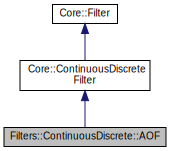
\includegraphics[width=242pt]{class_filters_1_1_continuous_discrete_1_1_a_o_f__inherit__graph}
\end{center}
\end{figure}


Граф связей класса Filters\+:\+:Continuous\+Discrete\+:\+:A\+OF\+:
\nopagebreak
\begin{figure}[H]
\begin{center}
\leavevmode
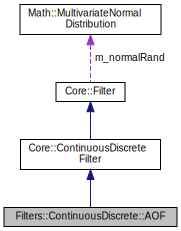
\includegraphics[width=242pt]{class_filters_1_1_continuous_discrete_1_1_a_o_f__coll__graph}
\end{center}
\end{figure}


\subsection{Методы}
\index{Filters\+::\+Continuous\+Discrete\+::\+A\+OF@{Filters\+::\+Continuous\+Discrete\+::\+A\+OF}!algorithm@{algorithm}}
\index{algorithm@{algorithm}!Filters\+::\+Continuous\+Discrete\+::\+A\+OF@{Filters\+::\+Continuous\+Discrete\+::\+A\+OF}}
\subsubsection[{\texorpdfstring{algorithm() override}{algorithm() override}}]{\setlength{\rightskip}{0pt plus 5cm}void Filters\+::\+Continuous\+Discrete\+::\+A\+O\+F\+::algorithm (
\begin{DoxyParamCaption}
{}
\end{DoxyParamCaption}
)\hspace{0.3cm}{\ttfamily [override]}, {\ttfamily [protected]}, {\ttfamily [virtual]}}\hypertarget{class_filters_1_1_continuous_discrete_1_1_a_o_f_a050849ffe1ada992988218805721914d}{}\label{class_filters_1_1_continuous_discrete_1_1_a_o_f_a050849ffe1ada992988218805721914d}


Выполняет алгоритм. 

Вектор $Z_t$ оценки между измерениями вычисляется из системы\+: \[\frac{d}{dt}Z_t = \tau(t,Z_t, P_t),\] \[\frac{d}{dt}P_t = A(t,Z_t, P_t) \cdot P_t + P_t \cdot A^T(t,Z_t, P_t) + \Theta(t,Z_t,P_t).\]

В моменты измерений\+: \[K_k = P_{t_k} \cdot G_k^T(Z_{t_k}, P_{t_k}) \cdot F_k^{-1}(Z_{t_k}, P_{t_k}),\] \[Z_{t_k^+} = Z_{t_k} + K_k \cdot [Y_k - h_k(Z_{t_k}, P_{t_k})],\] \[P_{t_k^+} = P_{t_k} - K_k \cdot G_k(Z_{t_k},P_{t_k}) \cdot P_{t_k}.\]

\begin{DoxySeeAlso}{См. также}
\hyperlink{class_core_1_1_continuous_discrete_filter}{Core\+::\+Continuous\+Discrete\+Filter} 

\hyperlink{class_core_1_1_continuous_discrete_task}{Core\+::\+Continuous\+Discrete\+Task} 
\end{DoxySeeAlso}


Замещает \hyperlink{class_core_1_1_filter_a438681ee3e54aba2148042d9f8011ab8}{Core\+::\+Filter}.



См. определение в файле cd\+\_\+aof.\+cc строка 31

\index{Filters\+::\+Continuous\+Discrete\+::\+A\+OF@{Filters\+::\+Continuous\+Discrete\+::\+A\+OF}!zero\+Iteration@{zero\+Iteration}}
\index{zero\+Iteration@{zero\+Iteration}!Filters\+::\+Continuous\+Discrete\+::\+A\+OF@{Filters\+::\+Continuous\+Discrete\+::\+A\+OF}}
\subsubsection[{\texorpdfstring{zero\+Iteration() override}{zeroIteration() override}}]{\setlength{\rightskip}{0pt plus 5cm}void Filters\+::\+Continuous\+Discrete\+::\+A\+O\+F\+::zero\+Iteration (
\begin{DoxyParamCaption}
{}
\end{DoxyParamCaption}
)\hspace{0.3cm}{\ttfamily [override]}, {\ttfamily [protected]}, {\ttfamily [virtual]}}\hypertarget{class_filters_1_1_continuous_discrete_1_1_a_o_f_ab350a4de87a9e2c2e8b01e178d61f3b5}{}\label{class_filters_1_1_continuous_discrete_1_1_a_o_f_ab350a4de87a9e2c2e8b01e178d61f3b5}


Нулевая итерация алгоритма (инициализирует начальные состояния). 

Практически для всех дискретных фильтров оптимальной структуры имеет вид\+: \[Z_0 = H_0 \cdot Y_0 + e_0,\] \[H_0 = D_{00}^{xy} \cdot (D_0^y)^{-1},\] \[e_0 = m_0^x - H_0 \cdot m_0^y.\]

В гауссовском АОФ (ФНА) добавляется уравнение для апостериорной ковариации объекта\+: \[P_0 = D_0^x - H_0 \cdot (D_{00}^{xy})^T.\] 

Переопределяет метод предка \hyperlink{class_core_1_1_continuous_discrete_filter_acc9b18241a13d46dc92ef1f02ec13e53}{Core\+::\+Continuous\+Discrete\+Filter}.



См. определение в файле cd\+\_\+aof.\+cc строка 21



\subsection{Данные класса}
\index{Filters\+::\+Continuous\+Discrete\+::\+A\+OF@{Filters\+::\+Continuous\+Discrete\+::\+A\+OF}!m\+\_\+sampleP@{m\+\_\+sampleP}}
\index{m\+\_\+sampleP@{m\+\_\+sampleP}!Filters\+::\+Continuous\+Discrete\+::\+A\+OF@{Filters\+::\+Continuous\+Discrete\+::\+A\+OF}}
\subsubsection[{\texorpdfstring{m\+\_\+sampleP}{m_sampleP}}]{\setlength{\rightskip}{0pt plus 5cm}Array$<$Matrix$>$ Filters\+::\+Continuous\+Discrete\+::\+A\+O\+F\+::m\+\_\+sampleP\hspace{0.3cm}{\ttfamily [protected]}}\hypertarget{class_filters_1_1_continuous_discrete_1_1_a_o_f_a31111852e94dab62675d8692a4c22df1}{}\label{class_filters_1_1_continuous_discrete_1_1_a_o_f_a31111852e94dab62675d8692a4c22df1}
Массив апостериорных ковариаций $P$. 

См. определение в файле cd\+\_\+aof.\+h строка 48



Объявления и описания членов классов находятся в файлах\+:\begin{DoxyCompactItemize}
\item 
src/filters/continuous\+\_\+discrete/cd\+\_\+aof.\+h\item 
src/filters/continuous\+\_\+discrete/cd\+\_\+aof.\+cc\end{DoxyCompactItemize}

\hypertarget{class_filters_1_1_discrete_1_1_a_o_f}{}\section{Класс Filters\+:\+:Discrete\+:\+:A\+OF}
\label{class_filters_1_1_discrete_1_1_a_o_f}\index{Filters\+::\+Discrete\+::\+A\+OF@{Filters\+::\+Discrete\+::\+A\+OF}}


Класс, реализующий дискретный абсолютно оптимальной фильтр.  




{\ttfamily \#include \char`\"{}d\+\_\+aof.\+h\char`\"{}}

\subsection*{Открытые члены}
\begin{DoxyCompactItemize}
\item 
\hypertarget{class_filters_1_1_discrete_1_1_a_o_f_a2df66ff12a7b327da999b0fd1dc82759}{}\label{class_filters_1_1_discrete_1_1_a_o_f_a2df66ff12a7b327da999b0fd1dc82759} 
\hyperlink{class_filters_1_1_discrete_1_1_a_o_f_a2df66ff12a7b327da999b0fd1dc82759}{A\+OF} (\hyperlink{namespace_core_a4811af8148ba137d644b9a61a042cf03}{Core\+::\+Ptr\+Filter\+Parameters} \hyperlink{class_core_1_1_filter_a44aa749b49ba46256975ce545531ecf7}{params}, \hyperlink{namespace_core_abfda8f69fcacfcea2696549b548ed737}{Core\+::\+Ptr\+Task} task)
\begin{DoxyCompactList}\small\item\em Конструктор. \end{DoxyCompactList}\end{DoxyCompactItemize}
\subsection*{Защищенные члены}
\begin{DoxyCompactItemize}
\item 
void \hyperlink{class_filters_1_1_discrete_1_1_a_o_f_aa822fe74d7ca160f898db1c1289e17f7}{zero\+Iteration} () override
\begin{DoxyCompactList}\small\item\em Нулевая итерация алгоритма (инициализирует начальные состояния). \end{DoxyCompactList}\item 
void \hyperlink{class_filters_1_1_discrete_1_1_a_o_f_a22cbbf1054a17045c5e91ed7c5cba387}{algorithm} () override
\begin{DoxyCompactList}\small\item\em Выполняет алгоритм. \end{DoxyCompactList}\end{DoxyCompactItemize}
\subsection*{Защищенные данные}
\begin{DoxyCompactItemize}
\item 
Array$<$ Matrix $>$ \hyperlink{class_filters_1_1_discrete_1_1_a_o_f_aef55ce0cf7129bb7090f8e470bcfbc1f}{m\+\_\+sampleP}
\end{DoxyCompactItemize}


\subsection{Подробное описание}
Класс, реализующий дискретный абсолютно оптимальной фильтр. 

См. определение в файле d\+\_\+aof.\+h строка 18



Граф наследования\+:Filters\+:\+:Discrete\+:\+:A\+OF\+:\nopagebreak
\begin{figure}[H]
\begin{center}
\leavevmode
\includegraphics[width=198pt]{class_filters_1_1_discrete_1_1_a_o_f__inherit__graph}
\end{center}
\end{figure}


Граф связей класса Filters\+:\+:Discrete\+:\+:A\+OF\+:\nopagebreak
\begin{figure}[H]
\begin{center}
\leavevmode
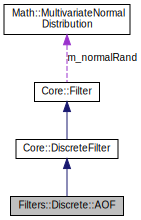
\includegraphics[width=198pt]{class_filters_1_1_discrete_1_1_a_o_f__coll__graph}
\end{center}
\end{figure}


\subsection{Методы}
\hypertarget{class_filters_1_1_discrete_1_1_a_o_f_a22cbbf1054a17045c5e91ed7c5cba387}{}\label{class_filters_1_1_discrete_1_1_a_o_f_a22cbbf1054a17045c5e91ed7c5cba387} 
\index{Filters\+::\+Discrete\+::\+A\+OF@{Filters\+::\+Discrete\+::\+A\+OF}!algorithm@{algorithm}}
\index{algorithm@{algorithm}!Filters\+::\+Discrete\+::\+A\+OF@{Filters\+::\+Discrete\+::\+A\+OF}}
\subsubsection{\texorpdfstring{algorithm()}{algorithm()}}
{\footnotesize\ttfamily void Filters\+::\+Discrete\+::\+A\+O\+F\+::algorithm (\begin{DoxyParamCaption}{ }\end{DoxyParamCaption})\hspace{0.3cm}{\ttfamily [override]}, {\ttfamily [protected]}, {\ttfamily [virtual]}}



Выполняет алгоритм. 

Вектор $Z_t$ оценки вычисляется следующим образом\+: \[\Lambda_k = \tau_{k-1}(Z_{k-1}, P_{k-1}),\] \[\Psi_k = \Theta_{k-1}(Z_{k-1}, P_{k-1}),\] \[H_k = \Psi_k \cdot G_k^T(\Lambda_k, \Psi_k) \cdot F_k^{-1}(\Lambda_k, \Psi_k),\] \[Z_k = \Lambda_k + H_k \cdot [Y_k - h_k(\Lambda_k, \Psi_k)],\] \[P_k = \Psi_k - H_k \cdot G_k(\Lambda_k, \Psi_k) \cdot \Psi_k.\]

\begin{DoxySeeAlso}{См. также}
\hyperlink{class_core_1_1_discrete_filter}{Core\+::\+Discrete\+Filter} 

\hyperlink{class_core_1_1_discrete_task}{Core\+::\+Discrete\+Task} 
\end{DoxySeeAlso}


Замещает \hyperlink{class_core_1_1_filter_a438681ee3e54aba2148042d9f8011ab8}{Core\+::\+Filter}.



См. определение в файле d\+\_\+aof.\+cc строка 37

\hypertarget{class_filters_1_1_discrete_1_1_a_o_f_aa822fe74d7ca160f898db1c1289e17f7}{}\label{class_filters_1_1_discrete_1_1_a_o_f_aa822fe74d7ca160f898db1c1289e17f7} 
\index{Filters\+::\+Discrete\+::\+A\+OF@{Filters\+::\+Discrete\+::\+A\+OF}!zero\+Iteration@{zero\+Iteration}}
\index{zero\+Iteration@{zero\+Iteration}!Filters\+::\+Discrete\+::\+A\+OF@{Filters\+::\+Discrete\+::\+A\+OF}}
\subsubsection{\texorpdfstring{zero\+Iteration()}{zeroIteration()}}
{\footnotesize\ttfamily void Filters\+::\+Discrete\+::\+A\+O\+F\+::zero\+Iteration (\begin{DoxyParamCaption}{ }\end{DoxyParamCaption})\hspace{0.3cm}{\ttfamily [override]}, {\ttfamily [protected]}, {\ttfamily [virtual]}}



Нулевая итерация алгоритма (инициализирует начальные состояния). 

Практически для всех дискретных фильтров оптимальной структуры имеет вид\+: \[Z_0 = H_0 \cdot Y_0 + e_0,\] \[H_0 = D_{00}^{xy} \cdot (D_0^y)^{-1},\] \[e_0 = m_0^x - H_0 \cdot m_0^y.\]

В гауссовском АОФ (ФНА) добавляется уравнение для апостериорной ковариации объекта\+: \[P_0 = D_0^x - H_0 \cdot (D_{00}^{xy})^T.\] 

Переопределяет метод предка \hyperlink{class_core_1_1_discrete_filter_a658617c64c7067bb6b98b5e9d78f982e}{Core\+::\+Discrete\+Filter}.



См. определение в файле d\+\_\+aof.\+cc строка 22



\subsection{Данные класса}
\hypertarget{class_filters_1_1_discrete_1_1_a_o_f_aef55ce0cf7129bb7090f8e470bcfbc1f}{}\label{class_filters_1_1_discrete_1_1_a_o_f_aef55ce0cf7129bb7090f8e470bcfbc1f} 
\index{Filters\+::\+Discrete\+::\+A\+OF@{Filters\+::\+Discrete\+::\+A\+OF}!m\+\_\+sampleP@{m\+\_\+sampleP}}
\index{m\+\_\+sampleP@{m\+\_\+sampleP}!Filters\+::\+Discrete\+::\+A\+OF@{Filters\+::\+Discrete\+::\+A\+OF}}
\subsubsection{\texorpdfstring{m\+\_\+sampleP}{m\_sampleP}}
{\footnotesize\ttfamily Array$<$Matrix$>$ Filters\+::\+Discrete\+::\+A\+O\+F\+::m\+\_\+sampleP\hspace{0.3cm}{\ttfamily [protected]}}

Массив апостериорных ковариаций $P$. 

См. определение в файле d\+\_\+aof.\+h строка 46



Объявления и описания членов классов находятся в файлах\+:\begin{DoxyCompactItemize}
\item 
src/filters/discrete/d\+\_\+aof.\+h\item 
src/filters/discrete/d\+\_\+aof.\+cc\end{DoxyCompactItemize}

\hypertarget{class_color_manager}{}\section{Класс Color\+Manager}
\label{class_color_manager}\index{Color\+Manager@{Color\+Manager}}


Класс для управления набором цветов.  




{\ttfamily \#include \char`\"{}color\+\_\+manager.\+h\char`\"{}}

\subsection*{Открытые члены}
\begin{DoxyCompactItemize}
\item 
\hyperlink{class_color_manager_a430efaaefd3650e29bcf4802394c29e9}{Color\+Manager} ()
\begin{DoxyCompactList}\small\item\em Конструктор. \end{DoxyCompactList}\item 
const Q\+Color \& \hyperlink{class_color_manager_ab7ace598efd321831f0924572a4bf84e}{next\+Color} ()\hypertarget{class_color_manager_ab7ace598efd321831f0924572a4bf84e}{}\label{class_color_manager_ab7ace598efd321831f0924572a4bf84e}

\begin{DoxyCompactList}\small\item\em Достает цвет из массива, сдвигает (циклически) индекс. \end{DoxyCompactList}\item 
void \hyperlink{class_color_manager_ae32d588a9d0144e2d55408c29f2f11ef}{reset} ()\hypertarget{class_color_manager_ae32d588a9d0144e2d55408c29f2f11ef}{}\label{class_color_manager_ae32d588a9d0144e2d55408c29f2f11ef}

\begin{DoxyCompactList}\small\item\em Сбрасывает индекс последнего извлеченного цвета до нулевого. \end{DoxyCompactList}\end{DoxyCompactItemize}
\subsection*{Закрытые данные}
\begin{DoxyCompactItemize}
\item 
int \hyperlink{class_color_manager_a7b6e45b4281881b4cf37a40dafd1a77a}{m\+\_\+current\+Index}
\item 
Q\+Vector$<$ Q\+Color $>$ \hyperlink{class_color_manager_ac91ea962bfa95bc3ed7da0bfd44615f4}{m\+\_\+colors}
\end{DoxyCompactItemize}


\subsection{Подробное описание}
Класс для управления набором цветов. 

См. определение в файле color\+\_\+manager.\+h строка 10



\subsection{Конструктор(ы)}
\index{Color\+Manager@{Color\+Manager}!Color\+Manager@{Color\+Manager}}
\index{Color\+Manager@{Color\+Manager}!Color\+Manager@{Color\+Manager}}
\subsubsection[{\texorpdfstring{Color\+Manager()}{ColorManager()}}]{\setlength{\rightskip}{0pt plus 5cm}Color\+Manager\+::\+Color\+Manager (
\begin{DoxyParamCaption}
{}
\end{DoxyParamCaption}
)}\hypertarget{class_color_manager_a430efaaefd3650e29bcf4802394c29e9}{}\label{class_color_manager_a430efaaefd3650e29bcf4802394c29e9}


Конструктор. 

Генерирует набор цветов и сохраняет его в массив.

Генерация происходит таким образом, чтобы соседние цвета были максимально \char`\"{}непохожими\char`\"{}. 

См. определение в файле color\+\_\+manager.\+cc строка 4



\subsection{Данные класса}
\index{Color\+Manager@{Color\+Manager}!m\+\_\+colors@{m\+\_\+colors}}
\index{m\+\_\+colors@{m\+\_\+colors}!Color\+Manager@{Color\+Manager}}
\subsubsection[{\texorpdfstring{m\+\_\+colors}{m_colors}}]{\setlength{\rightskip}{0pt plus 5cm}Q\+Vector$<$Q\+Color$>$ Color\+Manager\+::m\+\_\+colors\hspace{0.3cm}{\ttfamily [private]}}\hypertarget{class_color_manager_ac91ea962bfa95bc3ed7da0bfd44615f4}{}\label{class_color_manager_ac91ea962bfa95bc3ed7da0bfd44615f4}
Массив под набор цветов. 

См. определение в файле color\+\_\+manager.\+h строка 31

\index{Color\+Manager@{Color\+Manager}!m\+\_\+current\+Index@{m\+\_\+current\+Index}}
\index{m\+\_\+current\+Index@{m\+\_\+current\+Index}!Color\+Manager@{Color\+Manager}}
\subsubsection[{\texorpdfstring{m\+\_\+current\+Index}{m_currentIndex}}]{\setlength{\rightskip}{0pt plus 5cm}int Color\+Manager\+::m\+\_\+current\+Index\hspace{0.3cm}{\ttfamily [private]}}\hypertarget{class_color_manager_a7b6e45b4281881b4cf37a40dafd1a77a}{}\label{class_color_manager_a7b6e45b4281881b4cf37a40dafd1a77a}
Индекс последнего цвета, котороый \char`\"{}взяли\char`\"{}. 

См. определение в файле color\+\_\+manager.\+h строка 30



Объявления и описания членов классов находятся в файлах\+:\begin{DoxyCompactItemize}
\item 
src/gui/color\+\_\+manager.\+h\item 
src/gui/color\+\_\+manager.\+cc\end{DoxyCompactItemize}

\hypertarget{class_math_1_1_const}{}\section{Класс Math\+:\+:Const}
\label{class_math_1_1_const}\index{Math\+::\+Const@{Math\+::\+Const}}


Статический класс, содержащий константы.  




{\ttfamily \#include \char`\"{}constants.\+h\char`\"{}}

\subsection*{Статические открытые данные}
\begin{DoxyCompactItemize}
\item 
\hypertarget{class_math_1_1_const_af38bf8b7900394c82b8cc61d56a1d761}{}\label{class_math_1_1_const_af38bf8b7900394c82b8cc61d56a1d761} 
static constexpr double \hyperlink{class_math_1_1_const_af38bf8b7900394c82b8cc61d56a1d761}{PI} = 3.\+14159265358979323846264
\begin{DoxyCompactList}\small\item\em Число $\pi$. \end{DoxyCompactList}\item 
\hypertarget{class_math_1_1_const_a48120c3c268ef1ebb4533908ae0c920f}{}\label{class_math_1_1_const_a48120c3c268ef1ebb4533908ae0c920f} 
static constexpr double \hyperlink{class_math_1_1_const_a48120c3c268ef1ebb4533908ae0c920f}{E} = 2.\+71828182845904523536029
\begin{DoxyCompactList}\small\item\em Число $e$. \end{DoxyCompactList}\item 
\hypertarget{class_math_1_1_const_ad1d689a22e84a3c7e49a47cf80b3050f}{}\label{class_math_1_1_const_ad1d689a22e84a3c7e49a47cf80b3050f} 
static constexpr double \hyperlink{class_math_1_1_const_ad1d689a22e84a3c7e49a47cf80b3050f}{G\+A\+M\+MA} = 0.\+57721566490153286060651
\begin{DoxyCompactList}\small\item\em Постоянная Эйлера-\/Маскерони $\gamma$. \end{DoxyCompactList}\item 
\hypertarget{class_math_1_1_const_a7058de10aeb68c8ac5df5a7346278d15}{}\label{class_math_1_1_const_a7058de10aeb68c8ac5df5a7346278d15} 
static constexpr double \hyperlink{class_math_1_1_const_a7058de10aeb68c8ac5df5a7346278d15}{E\+PS} = std\+::numeric\+\_\+limits$<$double$>$\+::epsilon()
\begin{DoxyCompactList}\small\item\em Машинное $\epsilon$ для типа double. \end{DoxyCompactList}\item 
static constexpr double \hyperlink{class_math_1_1_const_a787c7176528a33522741da6b45761378}{M\+IN}
\begin{DoxyCompactList}\small\item\em Минимальное положительное значение для типа double. \end{DoxyCompactList}\item 
static constexpr double \hyperlink{class_math_1_1_const_aa6f0fbdf83bf388173d9712c2a9d2046}{M\+AX}
\begin{DoxyCompactList}\small\item\em Максимальное возможное значение для типа double. \end{DoxyCompactList}\item 
static constexpr double \hyperlink{class_math_1_1_const_a66b00ab50323d42c344eb25a680f1918}{I\+NF}
\begin{DoxyCompactList}\small\item\em Любое значение типа double, превышающее M\+AX. \end{DoxyCompactList}\end{DoxyCompactItemize}


\subsection{Подробное описание}
Статический класс, содержащий константы. 

См. определение в файле constants.\+h строка 14



\subsection{Данные класса}
\hypertarget{class_math_1_1_const_a66b00ab50323d42c344eb25a680f1918}{}\label{class_math_1_1_const_a66b00ab50323d42c344eb25a680f1918} 
\index{Math\+::\+Const@{Math\+::\+Const}!I\+NF@{I\+NF}}
\index{I\+NF@{I\+NF}!Math\+::\+Const@{Math\+::\+Const}}
\subsubsection{\texorpdfstring{I\+NF}{INF}}
{\footnotesize\ttfamily constexpr double Math\+::\+Const\+::\+I\+NF\hspace{0.3cm}{\ttfamily [static]}}

{\bfseries Инициализатор}
\begin{DoxyCode}
=
        std::numeric\_limits<double>::infinity()
\end{DoxyCode}


Любое значение типа double, превышающее M\+AX. 



См. определение в файле constants.\+h строка 25

\hypertarget{class_math_1_1_const_aa6f0fbdf83bf388173d9712c2a9d2046}{}\label{class_math_1_1_const_aa6f0fbdf83bf388173d9712c2a9d2046} 
\index{Math\+::\+Const@{Math\+::\+Const}!M\+AX@{M\+AX}}
\index{M\+AX@{M\+AX}!Math\+::\+Const@{Math\+::\+Const}}
\subsubsection{\texorpdfstring{M\+AX}{MAX}}
{\footnotesize\ttfamily constexpr double Math\+::\+Const\+::\+M\+AX\hspace{0.3cm}{\ttfamily [static]}}

{\bfseries Инициализатор}
\begin{DoxyCode}
=
        std::numeric\_limits<double>::max()
\end{DoxyCode}


Максимальное возможное значение для типа double. 



См. определение в файле constants.\+h строка 23

\hypertarget{class_math_1_1_const_a787c7176528a33522741da6b45761378}{}\label{class_math_1_1_const_a787c7176528a33522741da6b45761378} 
\index{Math\+::\+Const@{Math\+::\+Const}!M\+IN@{M\+IN}}
\index{M\+IN@{M\+IN}!Math\+::\+Const@{Math\+::\+Const}}
\subsubsection{\texorpdfstring{M\+IN}{MIN}}
{\footnotesize\ttfamily constexpr double Math\+::\+Const\+::\+M\+IN\hspace{0.3cm}{\ttfamily [static]}}

{\bfseries Инициализатор}
\begin{DoxyCode}
=
        std::numeric\_limits<double>::min()
\end{DoxyCode}


Минимальное положительное значение для типа double. 



См. определение в файле constants.\+h строка 21



Объявления и описания членов класса находятся в файле\+:\begin{DoxyCompactItemize}
\item 
src/math/constants.\+h\end{DoxyCompactItemize}

\hypertarget{class_core_1_1_continuous_discrete_filter}{}\section{Класс Core\+:\+:Continuous\+Discrete\+Filter}
\label{class_core_1_1_continuous_discrete_filter}\index{Core\+::\+Continuous\+Discrete\+Filter@{Core\+::\+Continuous\+Discrete\+Filter}}


Базовый класс для всех непрерывно-\/дискретных фильтров оптимальной структуры.  




{\ttfamily \#include \char`\"{}continuous\+\_\+discrete\+\_\+filter.\+h\char`\"{}}

\subsection*{Открытые члены}
\begin{DoxyCompactItemize}
\item 
\hypertarget{class_core_1_1_continuous_discrete_filter_a07811c4d421be2383961078cd07e6d96}{}\label{class_core_1_1_continuous_discrete_filter_a07811c4d421be2383961078cd07e6d96} 
\hyperlink{class_core_1_1_continuous_discrete_filter_a07811c4d421be2383961078cd07e6d96}{Continuous\+Discrete\+Filter} (\hyperlink{namespace_core_a4811af8148ba137d644b9a61a042cf03}{Ptr\+Filter\+Parameters} \hyperlink{class_core_1_1_filter_a44aa749b49ba46256975ce545531ecf7}{params}, \hyperlink{namespace_core_abfda8f69fcacfcea2696549b548ed737}{Ptr\+Task} task)
\begin{DoxyCompactList}\small\item\em Конструктор. \end{DoxyCompactList}\end{DoxyCompactItemize}
\subsection*{Защищенные члены}
\begin{DoxyCompactItemize}
\item 
void \hyperlink{class_core_1_1_continuous_discrete_filter_acc9b18241a13d46dc92ef1f02ec13e53}{zero\+Iteration} () override
\begin{DoxyCompactList}\small\item\em Нулевая итерация алгоритма (инициализирует начальные состояния). \end{DoxyCompactList}\end{DoxyCompactItemize}
\subsection*{Защищенные данные}
\begin{DoxyCompactItemize}
\item 
\hyperlink{namespace_core_a4d5939b0284102299f3fb63d7552826a}{Ptr\+C\+D\+Task} \hyperlink{class_core_1_1_continuous_discrete_filter_a14b9176c461ca407005e653ecc987b1b}{m\+\_\+task}
\end{DoxyCompactItemize}


\subsection{Подробное описание}
Базовый класс для всех непрерывно-\/дискретных фильтров оптимальной структуры. 

\begin{DoxySeeAlso}{См. также}
\hyperlink{class_core_1_1_continuous_discrete_task}{Continuous\+Discrete\+Task}. 
\end{DoxySeeAlso}


См. определение в файле continuous\+\_\+discrete\+\_\+filter.\+h строка 18



Граф наследования\+:Core\+:\+:Continuous\+Discrete\+Filter\+:\nopagebreak
\begin{figure}[H]
\begin{center}
\leavevmode
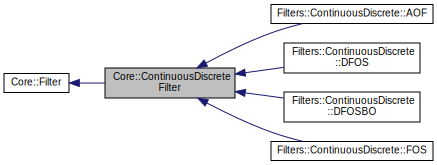
\includegraphics[width=350pt]{class_core_1_1_continuous_discrete_filter__inherit__graph}
\end{center}
\end{figure}


Граф связей класса Core\+:\+:Continuous\+Discrete\+Filter\+:\nopagebreak
\begin{figure}[H]
\begin{center}
\leavevmode
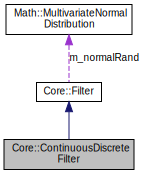
\includegraphics[width=220pt]{class_core_1_1_continuous_discrete_filter__coll__graph}
\end{center}
\end{figure}


\subsection{Методы}
\hypertarget{class_core_1_1_continuous_discrete_filter_acc9b18241a13d46dc92ef1f02ec13e53}{}\label{class_core_1_1_continuous_discrete_filter_acc9b18241a13d46dc92ef1f02ec13e53} 
\index{Core\+::\+Continuous\+Discrete\+Filter@{Core\+::\+Continuous\+Discrete\+Filter}!zero\+Iteration@{zero\+Iteration}}
\index{zero\+Iteration@{zero\+Iteration}!Core\+::\+Continuous\+Discrete\+Filter@{Core\+::\+Continuous\+Discrete\+Filter}}
\subsubsection{\texorpdfstring{zero\+Iteration()}{zeroIteration()}}
{\footnotesize\ttfamily void Core\+::\+Continuous\+Discrete\+Filter\+::zero\+Iteration (\begin{DoxyParamCaption}{ }\end{DoxyParamCaption})\hspace{0.3cm}{\ttfamily [override]}, {\ttfamily [protected]}, {\ttfamily [virtual]}}



Нулевая итерация алгоритма (инициализирует начальные состояния). 

Практически для всех дискретных фильтров оптимальной структуры имеет вид\+: \[Z_0 = H_0 \cdot Y_0 + e_0,\] \[H_0 = D_{00}^{xy} \cdot (D_0^y)^{-1},\] \[e_0 = m_0^x - H_0 \cdot m_0^y.\]

В гауссовском АОФ (ФНА) добавляется уравнение для апостериорной ковариации объекта\+: \[P_0 = D_0^x - H_0 \cdot (D_{00}^{xy})^T.\] 

Замещает \hyperlink{class_core_1_1_filter_af95880b734c4b8dc3d8c02f222b32506}{Core\+::\+Filter}.



Переопределяется в \hyperlink{class_filters_1_1_continuous_discrete_1_1_a_o_f_ab350a4de87a9e2c2e8b01e178d61f3b5}{Filters\+::\+Continuous\+Discrete\+::\+A\+OF} и \hyperlink{class_filters_1_1_continuous_discrete_1_1_d_f_o_s_b_o_a958c75df5031558a244d553f13376e75}{Filters\+::\+Continuous\+Discrete\+::\+D\+F\+O\+S\+BO}.



См. определение в файле continuous\+\_\+discrete\+\_\+filter.\+cc строка 21



\subsection{Данные класса}
\hypertarget{class_core_1_1_continuous_discrete_filter_a14b9176c461ca407005e653ecc987b1b}{}\label{class_core_1_1_continuous_discrete_filter_a14b9176c461ca407005e653ecc987b1b} 
\index{Core\+::\+Continuous\+Discrete\+Filter@{Core\+::\+Continuous\+Discrete\+Filter}!m\+\_\+task@{m\+\_\+task}}
\index{m\+\_\+task@{m\+\_\+task}!Core\+::\+Continuous\+Discrete\+Filter@{Core\+::\+Continuous\+Discrete\+Filter}}
\subsubsection{\texorpdfstring{m\+\_\+task}{m\_task}}
{\footnotesize\ttfamily \hyperlink{namespace_core_a4d5939b0284102299f3fb63d7552826a}{Ptr\+C\+D\+Task} Core\+::\+Continuous\+Discrete\+Filter\+::m\+\_\+task\hspace{0.3cm}{\ttfamily [protected]}}

Указатель на экземпляр задачи, с которой происходит работа. 

См. определение в файле continuous\+\_\+discrete\+\_\+filter.\+h строка 41



Объявления и описания членов классов находятся в файлах\+:\begin{DoxyCompactItemize}
\item 
src/core/continuous\+\_\+discrete\+\_\+filter.\+h\item 
src/core/continuous\+\_\+discrete\+\_\+filter.\+cc\end{DoxyCompactItemize}

\hypertarget{class_core_1_1_continuous_discrete_task}{}\section{Класс Core\+:\+:Continuous\+Discrete\+Task}
\label{class_core_1_1_continuous_discrete_task}\index{Core\+::\+Continuous\+Discrete\+Task@{Core\+::\+Continuous\+Discrete\+Task}}


Базовый тип задач для непрерывно-\/дискретных фильтров оптимальной структуры.  




{\ttfamily \#include \char`\"{}continuous\+\_\+discrete\+\_\+task.\+h\char`\"{}}

\subsection*{Открытые члены}
\begin{DoxyCompactItemize}
\item 
\hypertarget{class_core_1_1_continuous_discrete_task_a56d51edff4050c662197a16df126ca14}{}\label{class_core_1_1_continuous_discrete_task_a56d51edff4050c662197a16df126ca14} 
\hyperlink{class_core_1_1_continuous_discrete_task_a56d51edff4050c662197a16df126ca14}{Continuous\+Discrete\+Task} ()
\begin{DoxyCompactList}\small\item\em Конструктор. \end{DoxyCompactList}\item 
\hypertarget{class_core_1_1_continuous_discrete_task_a478f440555e63f6b14090637a6df46d9}{}\label{class_core_1_1_continuous_discrete_task_a478f440555e63f6b14090637a6df46d9} 
virtual Vector \hyperlink{class_core_1_1_continuous_discrete_task_a478f440555e63f6b14090637a6df46d9}{a} (const Vector \&x) const =0
\begin{DoxyCompactList}\small\item\em Функция сноса объекта $a(t,x)$. \end{DoxyCompactList}\item 
\hypertarget{class_core_1_1_continuous_discrete_task_acdecff4711bae9decda2931343929fae}{}\label{class_core_1_1_continuous_discrete_task_acdecff4711bae9decda2931343929fae} 
virtual Matrix \hyperlink{class_core_1_1_continuous_discrete_task_acdecff4711bae9decda2931343929fae}{B} (const Vector \&x) const =0
\begin{DoxyCompactList}\small\item\em Функция диффузии объекта $B(t,x)$. \end{DoxyCompactList}\item 
virtual Vector \hyperlink{class_core_1_1_continuous_discrete_task_a64ea27bc1e2a9e6bf1401fc7622c9aea}{c} (const Vector \&x) const =0
\begin{DoxyCompactList}\small\item\em Функция измерителя $c_k(X_k) = c_k(X_k, W_k)$. \end{DoxyCompactList}\item 
virtual Vector \hyperlink{class_core_1_1_continuous_discrete_task_a491a9dc4463031a6f5f2eeda24d8ba9c}{tau} (const Vector \&m, const Matrix \&D) const =0
\begin{DoxyCompactList}\small\item\em Структурная функция прогноза $\tau(t, m, D)$. \end{DoxyCompactList}\item 
virtual Matrix \hyperlink{class_core_1_1_continuous_discrete_task_a961cc49fd0c72ba0a211bb4913ca3ece}{Theta} (const Vector \&m, const Matrix \&D) const =0
\begin{DoxyCompactList}\small\item\em Структурная функция прогноза $\Theta(t,m,D)$. \end{DoxyCompactList}\item 
virtual Matrix \hyperlink{class_core_1_1_continuous_discrete_task_a332d99b61aabb919bffe75d0eec05cfe}{A} (const Vector \&m, const Matrix \&D) const =0
\begin{DoxyCompactList}\small\item\em Возвращает матрицу якоби $A(t, m, D)$ для функции $\tau(t, m, D)$. \end{DoxyCompactList}\item 
virtual Vector \hyperlink{class_core_1_1_continuous_discrete_task_a25e88b71eb477d99bad66a66c982af6f}{h} (const Vector \&m, const Matrix \&D) const =0
\begin{DoxyCompactList}\small\item\em Структурная функция коррекции $h_k(m, D)$. \end{DoxyCompactList}\item 
virtual Matrix \hyperlink{class_core_1_1_continuous_discrete_task_a2bc6d34d112ec0999857f7f9e0f67dda}{G} (const Vector \&m, const Matrix \&D) const =0
\begin{DoxyCompactList}\small\item\em Структурная функция коррекции $G_k(m, D)$. \end{DoxyCompactList}\item 
virtual Matrix \hyperlink{class_core_1_1_continuous_discrete_task_a08947ea4d4eb819e0e8530e682a1a377}{F} (const Vector \&m, const Matrix \&D) const =0
\begin{DoxyCompactList}\small\item\em Структурная функция коррекции $F_k(m, D)$. \end{DoxyCompactList}\end{DoxyCompactItemize}
\subsection*{Дополнительные унаследованные члены}


\subsection{Подробное описание}
Базовый тип задач для непрерывно-\/дискретных фильтров оптимальной структуры. 

Описываемая система имеет следующий вид


\begin{DoxyItemize}
\item Объект\+: \[dX_t = a(t, X_t)dt + B(t, X_t)dV_t,\ \ \ X_0 \sim \pi_0(x),\]
\item Измеритель\+: \[Y_k = с_k(X_{t_k}, W_k),\ \ \ k = 0, 1, \ldots\]
\end{DoxyItemize}

Здесь $t$ -\/ время, $t_k$ -\/ моменты измерений, $X_t = X(t)$ -\/ вектор состояния объекта в момент $t$, $Y_k$ -\/ вектор измерения, $V_t$ -\/ вектор стандартного винеровского процессов, $W_k$ -\/ вектор дискретного белого шума. 

См. определение в файле continuous\+\_\+discrete\+\_\+task.\+h строка 26



Граф наследования\+:Core\+:\+:Continuous\+Discrete\+Task\+:
\nopagebreak
\begin{figure}[H]
\begin{center}
\leavevmode
\includegraphics[width=350pt]{class_core_1_1_continuous_discrete_task__inherit__graph}
\end{center}
\end{figure}


Граф связей класса Core\+:\+:Continuous\+Discrete\+Task\+:
\nopagebreak
\begin{figure}[H]
\begin{center}
\leavevmode
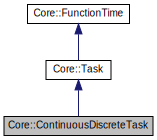
\includegraphics[width=229pt]{class_core_1_1_continuous_discrete_task__coll__graph}
\end{center}
\end{figure}


\subsection{Методы}
\hypertarget{class_core_1_1_continuous_discrete_task_a332d99b61aabb919bffe75d0eec05cfe}{}\label{class_core_1_1_continuous_discrete_task_a332d99b61aabb919bffe75d0eec05cfe} 
\index{Core\+::\+Continuous\+Discrete\+Task@{Core\+::\+Continuous\+Discrete\+Task}!A@{A}}
\index{A@{A}!Core\+::\+Continuous\+Discrete\+Task@{Core\+::\+Continuous\+Discrete\+Task}}
\subsubsection{\texorpdfstring{A()}{A()}}
{\footnotesize\ttfamily virtual Matrix Core\+::\+Continuous\+Discrete\+Task\+::A (\begin{DoxyParamCaption}\item[{const Vector \&}]{m,  }\item[{const Matrix \&}]{D }\end{DoxyParamCaption}) const\hspace{0.3cm}{\ttfamily [pure virtual]}}



Возвращает матрицу якоби $A(t, m, D)$ для функции $\tau(t, m, D)$. 

Она имеет следующий вид для


\begin{DoxyItemize}
\item гауссовского приближения\+: \[A(t, m, D) = \frac{d}{dm} \tau(t, m),\]
\item линеаризованного приближения\+: \[A(t, m, D) = \frac{d}{dm} a(t, m).\] 
\end{DoxyItemize}

Замещается в \hyperlink{class_tasks_1_1_continuous_discrete_1_1_landing_linear_ae584bc7b596882f07b18d2a39dcdfa32}{Tasks\+::\+Continuous\+Discrete\+::\+Landing\+Linear}, \hyperlink{class_tasks_1_1_continuous_discrete_1_1_van_der_pol_linear_abc0ead5ddd90702a5bbb93b07c74df85}{Tasks\+::\+Continuous\+Discrete\+::\+Van\+Der\+Pol\+Linear} и \hyperlink{class_tasks_1_1_continuous_discrete_1_1_van_der_pol_gauss_acb431d1a24b276610f6b7c7ff343fb9f}{Tasks\+::\+Continuous\+Discrete\+::\+Van\+Der\+Pol\+Gauss}.

\hypertarget{class_core_1_1_continuous_discrete_task_a64ea27bc1e2a9e6bf1401fc7622c9aea}{}\label{class_core_1_1_continuous_discrete_task_a64ea27bc1e2a9e6bf1401fc7622c9aea} 
\index{Core\+::\+Continuous\+Discrete\+Task@{Core\+::\+Continuous\+Discrete\+Task}!c@{c}}
\index{c@{c}!Core\+::\+Continuous\+Discrete\+Task@{Core\+::\+Continuous\+Discrete\+Task}}
\subsubsection{\texorpdfstring{c()}{c()}}
{\footnotesize\ttfamily virtual Vector Core\+::\+Continuous\+Discrete\+Task\+::c (\begin{DoxyParamCaption}\item[{const Vector \&}]{x }\end{DoxyParamCaption}) const\hspace{0.3cm}{\ttfamily [pure virtual]}}



Функция измерителя $c_k(X_k) = c_k(X_k, W_k)$. 

Шум $W_k$ генерируется внутри. 

Замещается в \hyperlink{class_tasks_1_1_continuous_discrete_1_1_landing_linear_aa3bddd1de01a202030bbccc1994e10af}{Tasks\+::\+Continuous\+Discrete\+::\+Landing\+Linear} и \hyperlink{class_tasks_1_1_continuous_discrete_1_1_van_der_pol_linear_af2602ff749602f29f5169ea0e1b391ed}{Tasks\+::\+Continuous\+Discrete\+::\+Van\+Der\+Pol\+Linear}.

\hypertarget{class_core_1_1_continuous_discrete_task_a08947ea4d4eb819e0e8530e682a1a377}{}\label{class_core_1_1_continuous_discrete_task_a08947ea4d4eb819e0e8530e682a1a377} 
\index{Core\+::\+Continuous\+Discrete\+Task@{Core\+::\+Continuous\+Discrete\+Task}!F@{F}}
\index{F@{F}!Core\+::\+Continuous\+Discrete\+Task@{Core\+::\+Continuous\+Discrete\+Task}}
\subsubsection{\texorpdfstring{F()}{F()}}
{\footnotesize\ttfamily virtual Matrix Core\+::\+Continuous\+Discrete\+Task\+::F (\begin{DoxyParamCaption}\item[{const Vector \&}]{m,  }\item[{const Matrix \&}]{D }\end{DoxyParamCaption}) const\hspace{0.3cm}{\ttfamily [pure virtual]}}



Структурная функция коррекции $F_k(m, D)$. 

Она имеет следующий вид для


\begin{DoxyItemize}
\item гауссовского приближения\+: \[F_k(m, D) = \int (M[c_k(x,W_k)\cdot c_k^T(x, W_k)] \cdot N(x\ |\ m,D))dx - h_k(m,D)\cdot h_k^T(m,D),\]
\item линеаризованного приближения\+: \[F_k(m, D) = C_k^x(m)\cdot D\cdot C_k^{xT}(m) + C_k^w(m)\cdot D[W_k]\cdot C_k^{wT}(m).\]
\end{DoxyItemize}

Здесь $C_k^x(x) = \frac{d}{dx} c_k(x, M[W_k]),\ C_k^w(x) = \frac{d}{dw} c_k(x, M[W_k])$. 

Замещается в \hyperlink{class_tasks_1_1_continuous_discrete_1_1_landing_linear_a5b5a327866160bf687dbc6d82a801ce8}{Tasks\+::\+Continuous\+Discrete\+::\+Landing\+Linear}, \hyperlink{class_tasks_1_1_continuous_discrete_1_1_van_der_pol_linear_ac624f91abb5e440d9b05835ca281f53f}{Tasks\+::\+Continuous\+Discrete\+::\+Van\+Der\+Pol\+Linear} и \hyperlink{class_tasks_1_1_continuous_discrete_1_1_van_der_pol_gauss_adbd6671eb347348b68db28d899484336}{Tasks\+::\+Continuous\+Discrete\+::\+Van\+Der\+Pol\+Gauss}.

\hypertarget{class_core_1_1_continuous_discrete_task_a2bc6d34d112ec0999857f7f9e0f67dda}{}\label{class_core_1_1_continuous_discrete_task_a2bc6d34d112ec0999857f7f9e0f67dda} 
\index{Core\+::\+Continuous\+Discrete\+Task@{Core\+::\+Continuous\+Discrete\+Task}!G@{G}}
\index{G@{G}!Core\+::\+Continuous\+Discrete\+Task@{Core\+::\+Continuous\+Discrete\+Task}}
\subsubsection{\texorpdfstring{G()}{G()}}
{\footnotesize\ttfamily virtual Matrix Core\+::\+Continuous\+Discrete\+Task\+::G (\begin{DoxyParamCaption}\item[{const Vector \&}]{m,  }\item[{const Matrix \&}]{D }\end{DoxyParamCaption}) const\hspace{0.3cm}{\ttfamily [pure virtual]}}



Структурная функция коррекции $G_k(m, D)$. 

Она имеет следующий вид для


\begin{DoxyItemize}
\item гауссовского приближения\+: \[G_k(m, D) = \frac{d}{dm}h_k(m,D),\]
\item линеаризованного приближения\+: \[G_k(m, D) = \frac{d}{dm}c_k(m,M[W_k]).\] 
\end{DoxyItemize}

Замещается в \hyperlink{class_tasks_1_1_continuous_discrete_1_1_landing_linear_a3b589b0ac53f7fe936438bc7c82f5c3d}{Tasks\+::\+Continuous\+Discrete\+::\+Landing\+Linear}, \hyperlink{class_tasks_1_1_continuous_discrete_1_1_van_der_pol_linear_aad1f3c80a043157b90ba0b55ba2390b1}{Tasks\+::\+Continuous\+Discrete\+::\+Van\+Der\+Pol\+Linear} и \hyperlink{class_tasks_1_1_continuous_discrete_1_1_van_der_pol_gauss_a757eb311b72b3cabcee59eab9d732de5}{Tasks\+::\+Continuous\+Discrete\+::\+Van\+Der\+Pol\+Gauss}.

\hypertarget{class_core_1_1_continuous_discrete_task_a25e88b71eb477d99bad66a66c982af6f}{}\label{class_core_1_1_continuous_discrete_task_a25e88b71eb477d99bad66a66c982af6f} 
\index{Core\+::\+Continuous\+Discrete\+Task@{Core\+::\+Continuous\+Discrete\+Task}!h@{h}}
\index{h@{h}!Core\+::\+Continuous\+Discrete\+Task@{Core\+::\+Continuous\+Discrete\+Task}}
\subsubsection{\texorpdfstring{h()}{h()}}
{\footnotesize\ttfamily virtual Vector Core\+::\+Continuous\+Discrete\+Task\+::h (\begin{DoxyParamCaption}\item[{const Vector \&}]{m,  }\item[{const Matrix \&}]{D }\end{DoxyParamCaption}) const\hspace{0.3cm}{\ttfamily [pure virtual]}}



Структурная функция коррекции $h_k(m, D)$. 

Она имеет следующий вид для


\begin{DoxyItemize}
\item гауссовского приближения\+: \[h_k(m, D) = \int (M[c_k(x, W_k)] \cdot N(x\ |\ m, D))dx,\]
\item линеаризованного приближения\+: \[h_k(m, D) = c_k(m, M[W_k]).\] 
\end{DoxyItemize}

Замещается в \hyperlink{class_tasks_1_1_continuous_discrete_1_1_landing_linear_a66480881fd719faddafe5104b548db78}{Tasks\+::\+Continuous\+Discrete\+::\+Landing\+Linear} и \hyperlink{class_tasks_1_1_continuous_discrete_1_1_van_der_pol_linear_a2a3ca4ebc2e8c458fbea40e854f375ec}{Tasks\+::\+Continuous\+Discrete\+::\+Van\+Der\+Pol\+Linear}.

\hypertarget{class_core_1_1_continuous_discrete_task_a491a9dc4463031a6f5f2eeda24d8ba9c}{}\label{class_core_1_1_continuous_discrete_task_a491a9dc4463031a6f5f2eeda24d8ba9c} 
\index{Core\+::\+Continuous\+Discrete\+Task@{Core\+::\+Continuous\+Discrete\+Task}!tau@{tau}}
\index{tau@{tau}!Core\+::\+Continuous\+Discrete\+Task@{Core\+::\+Continuous\+Discrete\+Task}}
\subsubsection{\texorpdfstring{tau()}{tau()}}
{\footnotesize\ttfamily virtual Vector Core\+::\+Continuous\+Discrete\+Task\+::tau (\begin{DoxyParamCaption}\item[{const Vector \&}]{m,  }\item[{const Matrix \&}]{D }\end{DoxyParamCaption}) const\hspace{0.3cm}{\ttfamily [pure virtual]}}



Структурная функция прогноза $\tau(t, m, D)$. 

Она имеет следующий вид для


\begin{DoxyItemize}
\item гауссовского приближения\+: \[\tau(t, m, D) = \int a(t,x)\cdot N(x\ |\ m, D)dx,\]
\item линеаризованного приближения\+: \[\tau(t, m, D) = a(t, m).\] 
\end{DoxyItemize}

Замещается в \hyperlink{class_tasks_1_1_continuous_discrete_1_1_landing_linear_a1ee11cced65180b2a055b8ca848ef4e0}{Tasks\+::\+Continuous\+Discrete\+::\+Landing\+Linear}, \hyperlink{class_tasks_1_1_continuous_discrete_1_1_van_der_pol_linear_a5b9245d9f403e615a971f2e8009926e6}{Tasks\+::\+Continuous\+Discrete\+::\+Van\+Der\+Pol\+Linear} и \hyperlink{class_tasks_1_1_continuous_discrete_1_1_van_der_pol_gauss_acfe935d9f4f452f3e10cb5f41fc8530a}{Tasks\+::\+Continuous\+Discrete\+::\+Van\+Der\+Pol\+Gauss}.

\hypertarget{class_core_1_1_continuous_discrete_task_a961cc49fd0c72ba0a211bb4913ca3ece}{}\label{class_core_1_1_continuous_discrete_task_a961cc49fd0c72ba0a211bb4913ca3ece} 
\index{Core\+::\+Continuous\+Discrete\+Task@{Core\+::\+Continuous\+Discrete\+Task}!Theta@{Theta}}
\index{Theta@{Theta}!Core\+::\+Continuous\+Discrete\+Task@{Core\+::\+Continuous\+Discrete\+Task}}
\subsubsection{\texorpdfstring{Theta()}{Theta()}}
{\footnotesize\ttfamily virtual Matrix Core\+::\+Continuous\+Discrete\+Task\+::\+Theta (\begin{DoxyParamCaption}\item[{const Vector \&}]{m,  }\item[{const Matrix \&}]{D }\end{DoxyParamCaption}) const\hspace{0.3cm}{\ttfamily [pure virtual]}}



Структурная функция прогноза $\Theta(t,m,D)$. 

Она имеет следующий вид для


\begin{DoxyItemize}
\item гауссовского приближения\+: \[\Theta(t,m,D) = \int B(t,x)\cdot B^T(t,x)\cdot N(x\ |\ m,D)dx,\]
\item линеаризованного приближения\+: \[\Theta(t,m,D) = B(t,m)\cdot B^T(t,m).\] 
\end{DoxyItemize}

Замещается в \hyperlink{class_tasks_1_1_continuous_discrete_1_1_landing_linear_a783147d41d5d8dff4facd246fc064bb4}{Tasks\+::\+Continuous\+Discrete\+::\+Landing\+Linear}, \hyperlink{class_tasks_1_1_continuous_discrete_1_1_van_der_pol_linear_a6d2f1c4c12551eda7eb97322335960ef}{Tasks\+::\+Continuous\+Discrete\+::\+Van\+Der\+Pol\+Linear} и \hyperlink{class_tasks_1_1_continuous_discrete_1_1_van_der_pol_gauss_addb8066d1f4701c0c453d07ffa8631ff}{Tasks\+::\+Continuous\+Discrete\+::\+Van\+Der\+Pol\+Gauss}.



Объявления и описания членов классов находятся в файлах\+:\begin{DoxyCompactItemize}
\item 
src/core/continuous\+\_\+discrete\+\_\+task.\+h\item 
src/core/continuous\+\_\+discrete\+\_\+task.\+cc\end{DoxyCompactItemize}

\hypertarget{class_core_1_1_continuous_filter}{}\section{Класс Core\+:\+:Continuous\+Filter}
\label{class_core_1_1_continuous_filter}\index{Core\+::\+Continuous\+Filter@{Core\+::\+Continuous\+Filter}}


Базовый класс для всех непрерывныз фильтров оптимальной структуры.  




{\ttfamily \#include \char`\"{}continuous\+\_\+filter.\+h\char`\"{}}

\subsection*{Открытые члены}
\begin{DoxyCompactItemize}
\item 
\hyperlink{class_core_1_1_continuous_filter_a5f28c1f5aaf740be3a6a8af09c0fcc22}{Continuous\+Filter} (\hyperlink{namespace_core_a4811af8148ba137d644b9a61a042cf03}{Ptr\+Filter\+Parameters} \hyperlink{class_core_1_1_filter_a44aa749b49ba46256975ce545531ecf7}{params}, \hyperlink{namespace_core_abfda8f69fcacfcea2696549b548ed737}{Ptr\+Task} task)\hypertarget{class_core_1_1_continuous_filter_a5f28c1f5aaf740be3a6a8af09c0fcc22}{}\label{class_core_1_1_continuous_filter_a5f28c1f5aaf740be3a6a8af09c0fcc22}

\begin{DoxyCompactList}\small\item\em Конструктор. \end{DoxyCompactList}\end{DoxyCompactItemize}
\subsection*{Защищенные члены}
\begin{DoxyCompactItemize}
\item 
void \hyperlink{class_core_1_1_continuous_filter_a4c30983f9354344717538f807855f2ae}{zero\+Iteration} () override
\begin{DoxyCompactList}\small\item\em Нулевая итерация алгоритма (инициализирует начальные состояния). \end{DoxyCompactList}\end{DoxyCompactItemize}
\subsection*{Защищенные данные}
\begin{DoxyCompactItemize}
\item 
\hyperlink{namespace_core_a95543587a560c6c497c6cadf68e03a62}{Ptr\+C\+Task} \hyperlink{class_core_1_1_continuous_filter_aaea7d47a9d573b9a88007780c4c3a722}{m\+\_\+task}
\end{DoxyCompactItemize}


\subsection{Подробное описание}
Базовый класс для всех непрерывныз фильтров оптимальной структуры. 

\begin{DoxySeeAlso}{См. также}
\hyperlink{class_core_1_1_continuous_task}{Continuous\+Task}. 
\end{DoxySeeAlso}


См. определение в файле continuous\+\_\+filter.\+h строка 17



Граф наследования\+:Core\+:\+:Continuous\+Filter\+:
\nopagebreak
\begin{figure}[H]
\begin{center}
\leavevmode
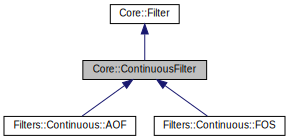
\includegraphics[width=348pt]{class_core_1_1_continuous_filter__inherit__graph}
\end{center}
\end{figure}


Граф связей класса Core\+:\+:Continuous\+Filter\+:
\nopagebreak
\begin{figure}[H]
\begin{center}
\leavevmode
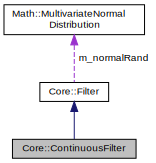
\includegraphics[width=213pt]{class_core_1_1_continuous_filter__coll__graph}
\end{center}
\end{figure}


\subsection{Методы}
\index{Core\+::\+Continuous\+Filter@{Core\+::\+Continuous\+Filter}!zero\+Iteration@{zero\+Iteration}}
\index{zero\+Iteration@{zero\+Iteration}!Core\+::\+Continuous\+Filter@{Core\+::\+Continuous\+Filter}}
\subsubsection[{\texorpdfstring{zero\+Iteration() override}{zeroIteration() override}}]{\setlength{\rightskip}{0pt plus 5cm}void Core\+::\+Continuous\+Filter\+::zero\+Iteration (
\begin{DoxyParamCaption}
{}
\end{DoxyParamCaption}
)\hspace{0.3cm}{\ttfamily [override]}, {\ttfamily [protected]}, {\ttfamily [virtual]}}\hypertarget{class_core_1_1_continuous_filter_a4c30983f9354344717538f807855f2ae}{}\label{class_core_1_1_continuous_filter_a4c30983f9354344717538f807855f2ae}


Нулевая итерация алгоритма (инициализирует начальные состояния). 

Практически для всех дискретных фильтров оптимальной структуры имеет вид\+: \[Z_0 = m_0^x = M[X_0],\]

В гауссовском АОФ (ФНА) добавляется уравнение для апостериорной ковариации объекта\+: \[P_0 = D_0^x = D[X_0].\] 

Замещает \hyperlink{class_core_1_1_filter_af95880b734c4b8dc3d8c02f222b32506}{Core\+::\+Filter}.



Переопределяется в \hyperlink{class_filters_1_1_continuous_1_1_a_o_f_ab416b56dbeb26366f495f03b3c08ad5e}{Filters\+::\+Continuous\+::\+A\+OF}.



См. определение в файле continuous\+\_\+filter.\+cc строка 19



\subsection{Данные класса}
\index{Core\+::\+Continuous\+Filter@{Core\+::\+Continuous\+Filter}!m\+\_\+task@{m\+\_\+task}}
\index{m\+\_\+task@{m\+\_\+task}!Core\+::\+Continuous\+Filter@{Core\+::\+Continuous\+Filter}}
\subsubsection[{\texorpdfstring{m\+\_\+task}{m_task}}]{\setlength{\rightskip}{0pt plus 5cm}{\bf Ptr\+C\+Task} Core\+::\+Continuous\+Filter\+::m\+\_\+task\hspace{0.3cm}{\ttfamily [protected]}}\hypertarget{class_core_1_1_continuous_filter_aaea7d47a9d573b9a88007780c4c3a722}{}\label{class_core_1_1_continuous_filter_aaea7d47a9d573b9a88007780c4c3a722}
Указатель на экземпляр задачи, с которой происходит работа. 

См. определение в файле continuous\+\_\+filter.\+h строка 38



Объявления и описания членов классов находятся в файлах\+:\begin{DoxyCompactItemize}
\item 
src/core/continuous\+\_\+filter.\+h\item 
src/core/continuous\+\_\+filter.\+cc\end{DoxyCompactItemize}

\hypertarget{class_core_1_1_continuous_task}{}\section{Класс Core\+:\+:Continuous\+Task}
\label{class_core_1_1_continuous_task}\index{Core\+::\+Continuous\+Task@{Core\+::\+Continuous\+Task}}


Базовый тип задач для непрерывных фильтров оптимальной структуры.  




{\ttfamily \#include \char`\"{}continuous\+\_\+task.\+h\char`\"{}}

\subsection*{Открытые члены}
\begin{DoxyCompactItemize}
\item 
\hypertarget{class_core_1_1_continuous_task_ab2c8106695e42db14d92364d1a310a6a}{}\label{class_core_1_1_continuous_task_ab2c8106695e42db14d92364d1a310a6a} 
\hyperlink{class_core_1_1_continuous_task_ab2c8106695e42db14d92364d1a310a6a}{Continuous\+Task} ()
\begin{DoxyCompactList}\small\item\em Конструктор. \end{DoxyCompactList}\item 
\hypertarget{class_core_1_1_continuous_task_a6117abb702d06b52eec1dc1951bab874}{}\label{class_core_1_1_continuous_task_a6117abb702d06b52eec1dc1951bab874} 
virtual Vector \hyperlink{class_core_1_1_continuous_task_a6117abb702d06b52eec1dc1951bab874}{a} (const Vector \&x) const =0
\begin{DoxyCompactList}\small\item\em Функция сноса объекта $a(t,x)$. \end{DoxyCompactList}\item 
\hypertarget{class_core_1_1_continuous_task_a1a1af322efd852451692b7a2e39ec19e}{}\label{class_core_1_1_continuous_task_a1a1af322efd852451692b7a2e39ec19e} 
virtual Matrix \hyperlink{class_core_1_1_continuous_task_a1a1af322efd852451692b7a2e39ec19e}{B} (const Vector \&x) const =0
\begin{DoxyCompactList}\small\item\em Функция диффузии объекта $B(t,x)$. \end{DoxyCompactList}\item 
\hypertarget{class_core_1_1_continuous_task_a623929970ce6d99f97b83b940003d004}{}\label{class_core_1_1_continuous_task_a623929970ce6d99f97b83b940003d004} 
virtual Vector \hyperlink{class_core_1_1_continuous_task_a623929970ce6d99f97b83b940003d004}{c} (const Vector \&x) const =0
\begin{DoxyCompactList}\small\item\em Функция сноса измерителя $с(t,x)$. \end{DoxyCompactList}\item 
\hypertarget{class_core_1_1_continuous_task_ac792d0a5d2487a30f9eb360344675173}{}\label{class_core_1_1_continuous_task_ac792d0a5d2487a30f9eb360344675173} 
virtual Matrix \hyperlink{class_core_1_1_continuous_task_ac792d0a5d2487a30f9eb360344675173}{D} (const Vector \&x) const =0
\begin{DoxyCompactList}\small\item\em Функция диффузии измерителя $D(t,x)$. \end{DoxyCompactList}\item 
virtual Matrix \hyperlink{class_core_1_1_continuous_task_a75fbac1abe67223cd7938b724c5cce45}{A} (const Vector \&m, const Matrix \&\hyperlink{class_core_1_1_continuous_task_ac792d0a5d2487a30f9eb360344675173}{D}) const =0
\begin{DoxyCompactList}\small\item\em Структурная функция $A(t, m, D)$. \end{DoxyCompactList}\item 
virtual Matrix \hyperlink{class_core_1_1_continuous_task_a1b579e183ffa229f97048aadfd834517}{G} (const Vector \&m, const Matrix \&\hyperlink{class_core_1_1_continuous_task_ac792d0a5d2487a30f9eb360344675173}{D}) const =0
\begin{DoxyCompactList}\small\item\em Структурная функция $G(t, m, D)$. \end{DoxyCompactList}\item 
virtual Matrix \hyperlink{class_core_1_1_continuous_task_aa6bc3b3c0c973169878c4e4b481dc922}{K} (const Vector \&m, const Matrix \&\hyperlink{class_core_1_1_continuous_task_ac792d0a5d2487a30f9eb360344675173}{D}) const
\begin{DoxyCompactList}\small\item\em Структурная функция $K(t, m, D)$. \end{DoxyCompactList}\item 
virtual Matrix \hyperlink{class_core_1_1_continuous_task_aaf28a2112c6e41e3ac4ff40c95ff71dd}{Psi} (const Vector \&m, const Matrix \&\hyperlink{class_core_1_1_continuous_task_ac792d0a5d2487a30f9eb360344675173}{D}) const
\begin{DoxyCompactList}\small\item\em Структурная функция $\Psi(t, m, D)$. \end{DoxyCompactList}\end{DoxyCompactItemize}
\subsection*{Защищенные члены}
\begin{DoxyCompactItemize}
\item 
\hypertarget{class_core_1_1_continuous_task_a8b3712283fb6a46c8c778c9e4f2045e2}{}\label{class_core_1_1_continuous_task_a8b3712283fb6a46c8c778c9e4f2045e2} 
virtual Matrix \hyperlink{class_core_1_1_continuous_task_a8b3712283fb6a46c8c778c9e4f2045e2}{Q} (const Vector \&m, const Matrix \&\hyperlink{class_core_1_1_continuous_task_ac792d0a5d2487a30f9eb360344675173}{D}) const =0
\begin{DoxyCompactList}\small\item\em Возвращает интенсивность шумов $Q(\cdot) = B(\cdot) \cdot B^T(\cdot)$. \end{DoxyCompactList}\item 
virtual Matrix \hyperlink{class_core_1_1_continuous_task_aa6d652b655628586aeeda03348f633c5}{S} (const Vector \&m, const Matrix \&\hyperlink{class_core_1_1_continuous_task_ac792d0a5d2487a30f9eb360344675173}{D}) const =0
\begin{DoxyCompactList}\small\item\em Возвращает интенсивность шумов $S(\cdot) = B(\cdot) \cdot D^T(\cdot)$. \end{DoxyCompactList}\item 
\hypertarget{class_core_1_1_continuous_task_ad98bb1adf1e394cac3f0bdead365f95a}{}\label{class_core_1_1_continuous_task_ad98bb1adf1e394cac3f0bdead365f95a} 
virtual Matrix \hyperlink{class_core_1_1_continuous_task_ad98bb1adf1e394cac3f0bdead365f95a}{R} (const Vector \&m, const Matrix \&\hyperlink{class_core_1_1_continuous_task_ac792d0a5d2487a30f9eb360344675173}{D}) const =0
\begin{DoxyCompactList}\small\item\em Возвращает интенсивность шумов $R(\cdot) = D(\cdot) \cdot D^T(\cdot)$. \end{DoxyCompactList}\end{DoxyCompactItemize}
\subsection*{Дополнительные унаследованные члены}


\subsection{Подробное описание}
Базовый тип задач для непрерывных фильтров оптимальной структуры. 

Описываемая система имеет следующий вид


\begin{DoxyItemize}
\item Объект\+: \[dX_t = a(t, X_t)dt + B(t, X_t)dV_t,\ \ \ X_0 \sim \pi_0(x),\]
\item Измеритель\+: \[dY_t = c_k(t, X_t) + D(t, X_t)dW_t,\ \ \ Y_0 = 0.\]
\end{DoxyItemize}

Здесь $t$ -\/ время, $X_t = X(t)$ -\/ вектор состояния объекта в момент $t$, $Y_t$ -\/ вектор измерения, $V_t, W_t$ -\/ векторы независимых стандартных винеровских процессов. 

См. определение в файле continuous\+\_\+task.\+h строка 25



Граф наследования\+:Core\+:\+:Continuous\+Task\+:\nopagebreak
\begin{figure}[H]
\begin{center}
\leavevmode
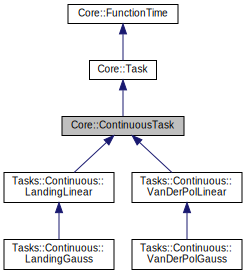
\includegraphics[width=306pt]{class_core_1_1_continuous_task__inherit__graph}
\end{center}
\end{figure}


Граф связей класса Core\+:\+:Continuous\+Task\+:\nopagebreak
\begin{figure}[H]
\begin{center}
\leavevmode
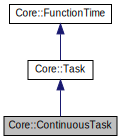
\includegraphics[width=193pt]{class_core_1_1_continuous_task__coll__graph}
\end{center}
\end{figure}


\subsection{Методы}
\hypertarget{class_core_1_1_continuous_task_a75fbac1abe67223cd7938b724c5cce45}{}\label{class_core_1_1_continuous_task_a75fbac1abe67223cd7938b724c5cce45} 
\index{Core\+::\+Continuous\+Task@{Core\+::\+Continuous\+Task}!A@{A}}
\index{A@{A}!Core\+::\+Continuous\+Task@{Core\+::\+Continuous\+Task}}
\subsubsection{\texorpdfstring{A()}{A()}}
{\footnotesize\ttfamily virtual Matrix Core\+::\+Continuous\+Task\+::A (\begin{DoxyParamCaption}\item[{const Vector \&}]{m,  }\item[{const Matrix \&}]{D }\end{DoxyParamCaption}) const\hspace{0.3cm}{\ttfamily [pure virtual]}}



Структурная функция $A(t, m, D)$. 

Она имеет следующий вид для


\begin{DoxyItemize}
\item линеаризованного приближения\+: \[A(t, m, D) = \frac{d}{dm} a(t, m).\] 
\end{DoxyItemize}

Замещается в \hyperlink{class_tasks_1_1_continuous_1_1_landing_linear_a8b06d0f38d73a27f7de0df6ba36b9c38}{Tasks\+::\+Continuous\+::\+Landing\+Linear}, \hyperlink{class_tasks_1_1_continuous_1_1_van_der_pol_linear_a2eefb5fca01c3517c44d2683032fda9d}{Tasks\+::\+Continuous\+::\+Van\+Der\+Pol\+Linear} и \hyperlink{class_tasks_1_1_continuous_1_1_van_der_pol_gauss_a2ef625f7f8c590726c5b52e67622c172}{Tasks\+::\+Continuous\+::\+Van\+Der\+Pol\+Gauss}.

\hypertarget{class_core_1_1_continuous_task_a1b579e183ffa229f97048aadfd834517}{}\label{class_core_1_1_continuous_task_a1b579e183ffa229f97048aadfd834517} 
\index{Core\+::\+Continuous\+Task@{Core\+::\+Continuous\+Task}!G@{G}}
\index{G@{G}!Core\+::\+Continuous\+Task@{Core\+::\+Continuous\+Task}}
\subsubsection{\texorpdfstring{G()}{G()}}
{\footnotesize\ttfamily virtual Matrix Core\+::\+Continuous\+Task\+::G (\begin{DoxyParamCaption}\item[{const Vector \&}]{m,  }\item[{const Matrix \&}]{D }\end{DoxyParamCaption}) const\hspace{0.3cm}{\ttfamily [pure virtual]}}



Структурная функция $G(t, m, D)$. 

Она имеет следующий вид для


\begin{DoxyItemize}
\item линеаризованного приближения\+: \[G(t, m, D) = \frac{d}{dm} c(t, m).\] 
\end{DoxyItemize}

Замещается в \hyperlink{class_tasks_1_1_continuous_1_1_landing_linear_af5937be9d9010e853956e5dd7ff96e8d}{Tasks\+::\+Continuous\+::\+Landing\+Linear}, \hyperlink{class_tasks_1_1_continuous_1_1_van_der_pol_linear_a931ba012a9671d8f522975232b48320f}{Tasks\+::\+Continuous\+::\+Van\+Der\+Pol\+Linear} и \hyperlink{class_tasks_1_1_continuous_1_1_van_der_pol_gauss_a1b61ca6de96df17b049bc7934a241e47}{Tasks\+::\+Continuous\+::\+Van\+Der\+Pol\+Gauss}.

\hypertarget{class_core_1_1_continuous_task_aa6bc3b3c0c973169878c4e4b481dc922}{}\label{class_core_1_1_continuous_task_aa6bc3b3c0c973169878c4e4b481dc922} 
\index{Core\+::\+Continuous\+Task@{Core\+::\+Continuous\+Task}!K@{K}}
\index{K@{K}!Core\+::\+Continuous\+Task@{Core\+::\+Continuous\+Task}}
\subsubsection{\texorpdfstring{K()}{K()}}
{\footnotesize\ttfamily Matrix Core\+::\+Continuous\+Task\+::K (\begin{DoxyParamCaption}\item[{const Vector \&}]{m,  }\item[{const Matrix \&}]{D }\end{DoxyParamCaption}) const\hspace{0.3cm}{\ttfamily [virtual]}}



Структурная функция $K(t, m, D)$. 

Она имеет следующий вид для


\begin{DoxyItemize}
\item линеаризованного приближения\+: \[K(t, m, D) = [D \cdot G^T(t,m) + S(t,m)] \cdot R^{-1}(t, m).\] 
\end{DoxyItemize}

См. определение в файле continuouse\+\_\+task.\+cc строка 15

\hypertarget{class_core_1_1_continuous_task_aaf28a2112c6e41e3ac4ff40c95ff71dd}{}\label{class_core_1_1_continuous_task_aaf28a2112c6e41e3ac4ff40c95ff71dd} 
\index{Core\+::\+Continuous\+Task@{Core\+::\+Continuous\+Task}!Psi@{Psi}}
\index{Psi@{Psi}!Core\+::\+Continuous\+Task@{Core\+::\+Continuous\+Task}}
\subsubsection{\texorpdfstring{Psi()}{Psi()}}
{\footnotesize\ttfamily Matrix Core\+::\+Continuous\+Task\+::\+Psi (\begin{DoxyParamCaption}\item[{const Vector \&}]{m,  }\item[{const Matrix \&}]{D }\end{DoxyParamCaption}) const\hspace{0.3cm}{\ttfamily [virtual]}}



Структурная функция $\Psi(t, m, D)$. 

Она имеет следующий вид для


\begin{DoxyItemize}
\item линеаризованного приближения\+: \[\Psi(t, m, D) = A(t,m)\cdot D + D \cdot A^T(t,m) + Q(t,m) - K(t,m,D) \cdot R(t,m) \cdot K^T(t,m,D).\] 
\end{DoxyItemize}

См. определение в файле continuouse\+\_\+task.\+cc строка 23

\hypertarget{class_core_1_1_continuous_task_aa6d652b655628586aeeda03348f633c5}{}\label{class_core_1_1_continuous_task_aa6d652b655628586aeeda03348f633c5} 
\index{Core\+::\+Continuous\+Task@{Core\+::\+Continuous\+Task}!S@{S}}
\index{S@{S}!Core\+::\+Continuous\+Task@{Core\+::\+Continuous\+Task}}
\subsubsection{\texorpdfstring{S()}{S()}}
{\footnotesize\ttfamily virtual Matrix Core\+::\+Continuous\+Task\+::S (\begin{DoxyParamCaption}\item[{const Vector \&}]{m,  }\item[{const Matrix \&}]{D }\end{DoxyParamCaption}) const\hspace{0.3cm}{\ttfamily [protected]}, {\ttfamily [pure virtual]}}



Возвращает интенсивность шумов $S(\cdot) = B(\cdot) \cdot D^T(\cdot)$. 

\begin{DoxyWarning}{Предупреждения}
Так как шумы независимые, то должна возвращать нулевую матрицу (нулевая взаимная интенсивность). 
\end{DoxyWarning}


Замещается в \hyperlink{class_tasks_1_1_continuous_1_1_landing_linear_a886bc6dd08e4355ab0c491d48f9de002}{Tasks\+::\+Continuous\+::\+Landing\+Linear} и \hyperlink{class_tasks_1_1_continuous_1_1_van_der_pol_linear_aa6cb67403faa3c2f894988aead527234}{Tasks\+::\+Continuous\+::\+Van\+Der\+Pol\+Linear}.



Объявления и описания членов классов находятся в файлах\+:\begin{DoxyCompactItemize}
\item 
src/core/continuous\+\_\+task.\+h\item 
src/core/continuouse\+\_\+task.\+cc\end{DoxyCompactItemize}

\hypertarget{class_math_1_1_lin_alg_1_1_current_pinv_method}{}\section{Класс Math\+:\+:Lin\+Alg\+:\+:Current\+Pinv\+Method}
\label{class_math_1_1_lin_alg_1_1_current_pinv_method}\index{Math\+::\+Lin\+Alg\+::\+Current\+Pinv\+Method@{Math\+::\+Lin\+Alg\+::\+Current\+Pinv\+Method}}


Класс, упрощающий выбор метода псевдообращения матриц.  




{\ttfamily \#include \char`\"{}linear\+\_\+algebra.\+h\char`\"{}}

\subsection*{Открытые члены}
\begin{DoxyCompactItemize}
\item 
\hypertarget{class_math_1_1_lin_alg_1_1_current_pinv_method_a6259004ad1c0c80f5798a3e7c12cf342}{}\label{class_math_1_1_lin_alg_1_1_current_pinv_method_a6259004ad1c0c80f5798a3e7c12cf342} 
\hyperlink{namespace_math_1_1_lin_alg_a34ee452c5d64eeb10e1bb63cf887af17}{Pseudoinverse\+Methods} \hyperlink{class_math_1_1_lin_alg_1_1_current_pinv_method_a6259004ad1c0c80f5798a3e7c12cf342}{get} () const
\begin{DoxyCompactList}\small\item\em Возвращает идентификатор выбранного метода. \end{DoxyCompactList}\item 
\hypertarget{class_math_1_1_lin_alg_1_1_current_pinv_method_ade16b67d5062f609bb8488f2ed78f0f3}{}\label{class_math_1_1_lin_alg_1_1_current_pinv_method_ade16b67d5062f609bb8488f2ed78f0f3} 
void \hyperlink{class_math_1_1_lin_alg_1_1_current_pinv_method_ade16b67d5062f609bb8488f2ed78f0f3}{set} (\hyperlink{namespace_math_1_1_lin_alg_a34ee452c5d64eeb10e1bb63cf887af17}{Pseudoinverse\+Methods} method)
\begin{DoxyCompactList}\small\item\em Устанавливает другой метод. \end{DoxyCompactList}\end{DoxyCompactItemize}
\subsection*{Открытые статические члены}
\begin{DoxyCompactItemize}
\item 
\hypertarget{class_math_1_1_lin_alg_1_1_current_pinv_method_a663575ba99f3a0a5359baacdcd410539}{}\label{class_math_1_1_lin_alg_1_1_current_pinv_method_a663575ba99f3a0a5359baacdcd410539} 
static \hyperlink{class_math_1_1_lin_alg_1_1_current_pinv_method}{Current\+Pinv\+Method} \& \hyperlink{class_math_1_1_lin_alg_1_1_current_pinv_method_a663575ba99f3a0a5359baacdcd410539}{instance} ()
\begin{DoxyCompactList}\small\item\em Возвращает ссылку на объект класса (singleton). \end{DoxyCompactList}\end{DoxyCompactItemize}
\subsection*{Закрытые члены}
\begin{DoxyCompactItemize}
\item 
\hypertarget{class_math_1_1_lin_alg_1_1_current_pinv_method_a21292458d8909e25f2c38999de7f07c3}{}\label{class_math_1_1_lin_alg_1_1_current_pinv_method_a21292458d8909e25f2c38999de7f07c3} 
\hyperlink{class_math_1_1_lin_alg_1_1_current_pinv_method_a21292458d8909e25f2c38999de7f07c3}{Current\+Pinv\+Method} ()
\begin{DoxyCompactList}\small\item\em Конструктор. \end{DoxyCompactList}\item 
\hypertarget{class_math_1_1_lin_alg_1_1_current_pinv_method_a41e66230275afe98d7c7a14dcf98e466}{}\label{class_math_1_1_lin_alg_1_1_current_pinv_method_a41e66230275afe98d7c7a14dcf98e466} 
{\bfseries Current\+Pinv\+Method} (const \hyperlink{class_math_1_1_lin_alg_1_1_current_pinv_method}{Current\+Pinv\+Method} \&)=delete
\item 
\hypertarget{class_math_1_1_lin_alg_1_1_current_pinv_method_a1b176bac6635060313ad235ef366cb8b}{}\label{class_math_1_1_lin_alg_1_1_current_pinv_method_a1b176bac6635060313ad235ef366cb8b} 
\hyperlink{class_math_1_1_lin_alg_1_1_current_pinv_method}{Current\+Pinv\+Method} \& {\bfseries operator=} (const \hyperlink{class_math_1_1_lin_alg_1_1_current_pinv_method}{Current\+Pinv\+Method} \&)=delete
\end{DoxyCompactItemize}
\subsection*{Закрытые данные}
\begin{DoxyCompactItemize}
\item 
\hypertarget{class_math_1_1_lin_alg_1_1_current_pinv_method_a38f44a507f0ade147651055746b2010e}{}\label{class_math_1_1_lin_alg_1_1_current_pinv_method_a38f44a507f0ade147651055746b2010e} 
\hyperlink{namespace_math_1_1_lin_alg_a34ee452c5d64eeb10e1bb63cf887af17}{Pseudoinverse\+Methods} {\bfseries m\+\_\+value}
\end{DoxyCompactItemize}


\subsection{Подробное описание}
Класс, упрощающий выбор метода псевдообращения матриц. 

См. определение в файле linear\+\_\+algebra.\+h строка 26



Объявления и описания членов классов находятся в файлах\+:\begin{DoxyCompactItemize}
\item 
src/math/linear\+\_\+algebra.\+h\item 
src/math/linear\+\_\+algebra.\+cc\end{DoxyCompactItemize}

\hypertarget{class_filters_1_1_continuous_discrete_1_1_d_f_o_s}{}\section{Класс Filters\+:\+:Continuous\+Discrete\+:\+:D\+F\+OS}
\label{class_filters_1_1_continuous_discrete_1_1_d_f_o_s}\index{Filters\+::\+Continuous\+Discrete\+::\+D\+F\+OS@{Filters\+::\+Continuous\+Discrete\+::\+D\+F\+OS}}


Класс, реализующий непрерывно-\/дискретный фильтр оптимальной структуры с дискретным прогнозом.  




{\ttfamily \#include \char`\"{}cd\+\_\+dfos.\+h\char`\"{}}

\subsection*{Открытые члены}
\begin{DoxyCompactItemize}
\item 
\hypertarget{class_filters_1_1_continuous_discrete_1_1_d_f_o_s_a962505dc3f59ef8b68cb228b1cf481f1}{}\label{class_filters_1_1_continuous_discrete_1_1_d_f_o_s_a962505dc3f59ef8b68cb228b1cf481f1} 
\hyperlink{class_filters_1_1_continuous_discrete_1_1_d_f_o_s_a962505dc3f59ef8b68cb228b1cf481f1}{D\+F\+OS} (\hyperlink{namespace_core_a4811af8148ba137d644b9a61a042cf03}{Core\+::\+Ptr\+Filter\+Parameters} \hyperlink{class_core_1_1_filter_a44aa749b49ba46256975ce545531ecf7}{params}, \hyperlink{namespace_core_abfda8f69fcacfcea2696549b548ed737}{Core\+::\+Ptr\+Task} task)
\begin{DoxyCompactList}\small\item\em Конструктор. \end{DoxyCompactList}\end{DoxyCompactItemize}
\subsection*{Защищенные члены}
\begin{DoxyCompactItemize}
\item 
void \hyperlink{class_filters_1_1_continuous_discrete_1_1_d_f_o_s_a532847e55043544b0ea50fd5744939c1}{algorithm} () override
\begin{DoxyCompactList}\small\item\em Выполняет алгоритм. \end{DoxyCompactList}\end{DoxyCompactItemize}
\subsection*{Дополнительные унаследованные члены}


\subsection{Подробное описание}
Класс, реализующий непрерывно-\/дискретный фильтр оптимальной структуры с дискретным прогнозом. 

См. определение в файле cd\+\_\+dfos.\+h строка 16



Граф наследования\+:Filters\+:\+:Continuous\+Discrete\+:\+:D\+F\+OS\+:
\nopagebreak
\begin{figure}[H]
\begin{center}
\leavevmode
\includegraphics[width=227pt]{class_filters_1_1_continuous_discrete_1_1_d_f_o_s__inherit__graph}
\end{center}
\end{figure}


Граф связей класса Filters\+:\+:Continuous\+Discrete\+:\+:D\+F\+OS\+:
\nopagebreak
\begin{figure}[H]
\begin{center}
\leavevmode
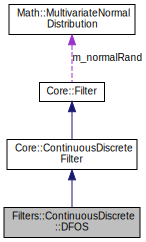
\includegraphics[width=232pt]{class_filters_1_1_continuous_discrete_1_1_d_f_o_s__coll__graph}
\end{center}
\end{figure}


\subsection{Методы}
\hypertarget{class_filters_1_1_continuous_discrete_1_1_d_f_o_s_a532847e55043544b0ea50fd5744939c1}{}\label{class_filters_1_1_continuous_discrete_1_1_d_f_o_s_a532847e55043544b0ea50fd5744939c1} 
\index{Filters\+::\+Continuous\+Discrete\+::\+D\+F\+OS@{Filters\+::\+Continuous\+Discrete\+::\+D\+F\+OS}!algorithm@{algorithm}}
\index{algorithm@{algorithm}!Filters\+::\+Continuous\+Discrete\+::\+D\+F\+OS@{Filters\+::\+Continuous\+Discrete\+::\+D\+F\+OS}}
\subsubsection{\texorpdfstring{algorithm()}{algorithm()}}
{\footnotesize\ttfamily void Filters\+::\+Continuous\+Discrete\+::\+D\+F\+O\+S\+::algorithm (\begin{DoxyParamCaption}{ }\end{DoxyParamCaption})\hspace{0.3cm}{\ttfamily [override]}, {\ttfamily [protected]}, {\ttfamily [virtual]}}



Выполняет алгоритм. 

Вектор $Z_t$ оценки между измерениями (прогнозирование) вычисляется следующим образом\+: \[Z_{\tau_k^i} = \Gamma_k^i \cdot Z_{\tau_k^{i-1}} + \kappa_k^i,\ \ \ i = 1 \ldots L,\]

В моменты измерений\+: \[\Lambda_k = \Gamma_k \cdot Z_{\tau_{k-1}^L} + \kappa_k,\] \[Z_{\tau_k^0} = \Lambda_k + T_k \cdot G_k^T(\Lambda_k, T_k) \cdot F_k^{-1}(\Lambda_k, T_k) \cdot [Y_k - h_k(\Lambda_k, T_k)],\]

Параметры вычисляется так\+: \[\Gamma_k^i = D_{\tau_k^i,\tau_k^{i-1}}^{x,z} \cdot (D_{\tau_k^{i-1}}^z)^{-1},\ \ \kappa_k^i = m_{\tau_k^i}^x - \Gamma_k^i \cdot m_{\tau_k^{i-1}}^z,\] \[\Gamma_k = D_{t_k,\tau_{k-1}^L}^{x,z} \cdot (D_{\tau_{k-1}^L}^z)^{-1},\ \ \kappa_k = m_{t_k}^x - \Gamma_k \cdot m_{\tau_{k-1}^L}^z,\] \[T_k = D_{t_k}^x - \Gamma_k \cdot (D_{t_k,\tau_{k-1}^L}^{x,z})^T.\]

\begin{DoxySeeAlso}{См. также}
\hyperlink{class_core_1_1_continuous_discrete_filter}{Core\+::\+Continuous\+Discrete\+Filter} 

\hyperlink{class_core_1_1_continuous_discrete_task}{Core\+::\+Continuous\+Discrete\+Task} 
\end{DoxySeeAlso}


Замещает \hyperlink{class_core_1_1_filter_a438681ee3e54aba2148042d9f8011ab8}{Core\+::\+Filter}.



См. определение в файле cd\+\_\+dfos.\+cc строка 21



Объявления и описания членов классов находятся в файлах\+:\begin{DoxyCompactItemize}
\item 
src/filters/continuous\+\_\+discrete/cd\+\_\+dfos.\+h\item 
src/filters/continuous\+\_\+discrete/cd\+\_\+dfos.\+cc\end{DoxyCompactItemize}

\hypertarget{class_filters_1_1_continuous_discrete_1_1_d_f_o_s_b_o}{}\section{Класс Filters\+:\+:Continuous\+Discrete\+:\+:D\+F\+O\+S\+BO}
\label{class_filters_1_1_continuous_discrete_1_1_d_f_o_s_b_o}\index{Filters\+::\+Continuous\+Discrete\+::\+D\+F\+O\+S\+BO@{Filters\+::\+Continuous\+Discrete\+::\+D\+F\+O\+S\+BO}}


Класс, реализующий непрерывно-\/дискретный фильтр оптимальной структуры повышеного порядка.  




{\ttfamily \#include \char`\"{}cd\+\_\+dfosbo.\+h\char`\"{}}

\subsection*{Открытые члены}
\begin{DoxyCompactItemize}
\item 
\hypertarget{class_filters_1_1_continuous_discrete_1_1_d_f_o_s_b_o_acadfa83ce71342e673d5cf954bda3cdc}{}\label{class_filters_1_1_continuous_discrete_1_1_d_f_o_s_b_o_acadfa83ce71342e673d5cf954bda3cdc} 
\hyperlink{class_filters_1_1_continuous_discrete_1_1_d_f_o_s_b_o_acadfa83ce71342e673d5cf954bda3cdc}{D\+F\+O\+S\+BO} (\hyperlink{namespace_core_a4811af8148ba137d644b9a61a042cf03}{Core\+::\+Ptr\+Filter\+Parameters} \hyperlink{class_core_1_1_filter_a44aa749b49ba46256975ce545531ecf7}{params}, \hyperlink{namespace_core_abfda8f69fcacfcea2696549b548ed737}{Core\+::\+Ptr\+Task} task)
\begin{DoxyCompactList}\small\item\em Конструктор. \end{DoxyCompactList}\end{DoxyCompactItemize}
\subsection*{Защищенные члены}
\begin{DoxyCompactItemize}
\item 
void \hyperlink{class_filters_1_1_continuous_discrete_1_1_d_f_o_s_b_o_a958c75df5031558a244d553f13376e75}{zero\+Iteration} () override
\begin{DoxyCompactList}\small\item\em Нулевая итерация алгоритма (инициализирует начальные состояния). \end{DoxyCompactList}\item 
void \hyperlink{class_filters_1_1_continuous_discrete_1_1_d_f_o_s_b_o_ab911983ab9ff8e22dc68e33fdb4601b6}{algorithm} () override
\begin{DoxyCompactList}\small\item\em Выполняет алгоритм. \end{DoxyCompactList}\end{DoxyCompactItemize}
\subsection*{Защищенные данные}
\begin{DoxyCompactItemize}
\item 
Array$<$ Vector $>$ \hyperlink{class_filters_1_1_continuous_discrete_1_1_d_f_o_s_b_o_affccb91872f23878db490d487c481606}{m\+\_\+sampleS}
\end{DoxyCompactItemize}


\subsection{Подробное описание}
Класс, реализующий непрерывно-\/дискретный фильтр оптимальной структуры повышеного порядка. 

См. определение в файле cd\+\_\+dfosbo.\+h строка 16



Граф наследования\+:Filters\+:\+:Continuous\+Discrete\+:\+:D\+F\+O\+S\+BO\+:\nopagebreak
\begin{figure}[H]
\begin{center}
\leavevmode
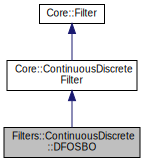
\includegraphics[width=227pt]{class_filters_1_1_continuous_discrete_1_1_d_f_o_s_b_o__inherit__graph}
\end{center}
\end{figure}


Граф связей класса Filters\+:\+:Continuous\+Discrete\+:\+:D\+F\+O\+S\+BO\+:\nopagebreak
\begin{figure}[H]
\begin{center}
\leavevmode
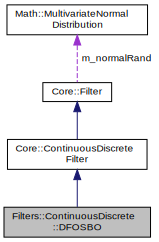
\includegraphics[width=227pt]{class_filters_1_1_continuous_discrete_1_1_d_f_o_s_b_o__coll__graph}
\end{center}
\end{figure}


\subsection{Методы}
\hypertarget{class_filters_1_1_continuous_discrete_1_1_d_f_o_s_b_o_ab911983ab9ff8e22dc68e33fdb4601b6}{}\label{class_filters_1_1_continuous_discrete_1_1_d_f_o_s_b_o_ab911983ab9ff8e22dc68e33fdb4601b6} 
\index{Filters\+::\+Continuous\+Discrete\+::\+D\+F\+O\+S\+BO@{Filters\+::\+Continuous\+Discrete\+::\+D\+F\+O\+S\+BO}!algorithm@{algorithm}}
\index{algorithm@{algorithm}!Filters\+::\+Continuous\+Discrete\+::\+D\+F\+O\+S\+BO@{Filters\+::\+Continuous\+Discrete\+::\+D\+F\+O\+S\+BO}}
\subsubsection{\texorpdfstring{algorithm()}{algorithm()}}
{\footnotesize\ttfamily void Filters\+::\+Continuous\+Discrete\+::\+D\+F\+O\+S\+B\+O\+::algorithm (\begin{DoxyParamCaption}{ }\end{DoxyParamCaption})\hspace{0.3cm}{\ttfamily [override]}, {\ttfamily [protected]}, {\ttfamily [virtual]}}



Выполняет алгоритм. 

Алгоритм схож с \hyperlink{class_filters_1_1_continuous_discrete_1_1_d_f_o_s}{D\+F\+OS}. Отличие в вычислении вектора состояния между измерениями (прогнозы).

Вводится расширенный вектор состояния $S_k$\+: \[ S_k = [Y_k^T\ \ Y_{k-1}^T\ \cdots Y_{k-l+1}^T]^T,\] где $l$ -\/ кратность порядка $p = l \cdot dim(Y)$ фильтра.

Вектор $Z_t$ оценки между измерениями (прогнозирование) вычисляется следующим образом\+: \[Z_{\tau_k^i} = \Gamma_k^i \cdot S_k + \kappa_k^i,\ \ \ i = 1 \ldots L,\]

В моменты измерений\+: \[\Lambda_k = \Gamma_k \cdot Z_{k-1} + \kappa_k,\] \[Z_{\tau_k^0} = \Lambda_k + T_k \cdot G_k^T(\Lambda_k, T_k) \cdot F_k^{-1}(\Lambda_k, T_k) \cdot [Y_k - h_k(\Lambda_k, T_k)],\]

Параметры вычисляется так\+: \[\Gamma_k^i = D_{\tau_k^i,k}^{x,s} \cdot (D_k^s)^{-1},\ \ \kappa_k^i = m_{\tau_k^i}^x - \Gamma_k^i \cdot m_k^s,\] \[\Gamma_k = D_{\tau_k^0,k-1}^{x,s} \cdot (D_{k-1}^s)^{-1},\ \ \kappa_k = m_{\tau_k^0}^x - \Gamma_k \cdot m_{k-1}^s,\] \[T_k = D_{\tau_k^0}^x - \Gamma_k \cdot (D_{\tau_k^0,k-1}^{x,s})^T.\]

\begin{DoxySeeAlso}{См. также}
\hyperlink{class_core_1_1_continuous_discrete_filter}{Core\+::\+Continuous\+Discrete\+Filter} 

\hyperlink{class_core_1_1_continuous_discrete_task}{Core\+::\+Continuous\+Discrete\+Task} 
\end{DoxySeeAlso}


Замещает \hyperlink{class_core_1_1_filter_a438681ee3e54aba2148042d9f8011ab8}{Core\+::\+Filter}.



См. определение в файле cd\+\_\+dfosbo.\+cc строка 42

\hypertarget{class_filters_1_1_continuous_discrete_1_1_d_f_o_s_b_o_a958c75df5031558a244d553f13376e75}{}\label{class_filters_1_1_continuous_discrete_1_1_d_f_o_s_b_o_a958c75df5031558a244d553f13376e75} 
\index{Filters\+::\+Continuous\+Discrete\+::\+D\+F\+O\+S\+BO@{Filters\+::\+Continuous\+Discrete\+::\+D\+F\+O\+S\+BO}!zero\+Iteration@{zero\+Iteration}}
\index{zero\+Iteration@{zero\+Iteration}!Filters\+::\+Continuous\+Discrete\+::\+D\+F\+O\+S\+BO@{Filters\+::\+Continuous\+Discrete\+::\+D\+F\+O\+S\+BO}}
\subsubsection{\texorpdfstring{zero\+Iteration()}{zeroIteration()}}
{\footnotesize\ttfamily void Filters\+::\+Continuous\+Discrete\+::\+D\+F\+O\+S\+B\+O\+::zero\+Iteration (\begin{DoxyParamCaption}{ }\end{DoxyParamCaption})\hspace{0.3cm}{\ttfamily [override]}, {\ttfamily [protected]}, {\ttfamily [virtual]}}



Нулевая итерация алгоритма (инициализирует начальные состояния). 

Практически для всех дискретных фильтров оптимальной структуры имеет вид\+: \[Z_0 = H_0 \cdot Y_0 + e_0,\] \[H_0 = D_{00}^{xy} \cdot (D_0^y)^{-1},\] \[e_0 = m_0^x - H_0 \cdot m_0^y.\]

В гауссовском АОФ (ФНА) добавляется уравнение для апостериорной ковариации объекта\+: \[P_0 = D_0^x - H_0 \cdot (D_{00}^{xy})^T.\] 

Переопределяет метод предка \hyperlink{class_core_1_1_continuous_discrete_filter_acc9b18241a13d46dc92ef1f02ec13e53}{Core\+::\+Continuous\+Discrete\+Filter}.



См. определение в файле cd\+\_\+dfosbo.\+cc строка 25



\subsection{Данные класса}
\hypertarget{class_filters_1_1_continuous_discrete_1_1_d_f_o_s_b_o_affccb91872f23878db490d487c481606}{}\label{class_filters_1_1_continuous_discrete_1_1_d_f_o_s_b_o_affccb91872f23878db490d487c481606} 
\index{Filters\+::\+Continuous\+Discrete\+::\+D\+F\+O\+S\+BO@{Filters\+::\+Continuous\+Discrete\+::\+D\+F\+O\+S\+BO}!m\+\_\+sampleS@{m\+\_\+sampleS}}
\index{m\+\_\+sampleS@{m\+\_\+sampleS}!Filters\+::\+Continuous\+Discrete\+::\+D\+F\+O\+S\+BO@{Filters\+::\+Continuous\+Discrete\+::\+D\+F\+O\+S\+BO}}
\subsubsection{\texorpdfstring{m\+\_\+sampleS}{m\_sampleS}}
{\footnotesize\ttfamily Array$<$Vector$>$ Filters\+::\+Continuous\+Discrete\+::\+D\+F\+O\+S\+B\+O\+::m\+\_\+sampleS\hspace{0.3cm}{\ttfamily [protected]}}

Массив для хранения расширенных векторов состояния $S_k$. 

См. определение в файле cd\+\_\+dfosbo.\+h строка 58



Объявления и описания членов классов находятся в файлах\+:\begin{DoxyCompactItemize}
\item 
src/filters/continuous\+\_\+discrete/cd\+\_\+dfosbo.\+h\item 
src/filters/continuous\+\_\+discrete/cd\+\_\+dfosbo.\+cc\end{DoxyCompactItemize}

\hypertarget{class_core_1_1_discrete_filter}{}\section{Класс Core\+:\+:Discrete\+Filter}
\label{class_core_1_1_discrete_filter}\index{Core\+::\+Discrete\+Filter@{Core\+::\+Discrete\+Filter}}


Базовый класс для всех дискретных фильтров оптимальной структуры.  




{\ttfamily \#include \char`\"{}discrete\+\_\+filter.\+h\char`\"{}}

\subsection*{Открытые члены}
\begin{DoxyCompactItemize}
\item 
\hypertarget{class_core_1_1_discrete_filter_a87399ba405c2dfe8037191fe907df141}{}\label{class_core_1_1_discrete_filter_a87399ba405c2dfe8037191fe907df141} 
\hyperlink{class_core_1_1_discrete_filter_a87399ba405c2dfe8037191fe907df141}{Discrete\+Filter} (\hyperlink{namespace_core_a4811af8148ba137d644b9a61a042cf03}{Ptr\+Filter\+Parameters} \hyperlink{class_core_1_1_filter_a44aa749b49ba46256975ce545531ecf7}{params}, \hyperlink{namespace_core_abfda8f69fcacfcea2696549b548ed737}{Ptr\+Task} task)
\begin{DoxyCompactList}\small\item\em Конструктор. \end{DoxyCompactList}\end{DoxyCompactItemize}
\subsection*{Защищенные члены}
\begin{DoxyCompactItemize}
\item 
void \hyperlink{class_core_1_1_discrete_filter_a658617c64c7067bb6b98b5e9d78f982e}{zero\+Iteration} () override
\begin{DoxyCompactList}\small\item\em Нулевая итерация алгоритма (инициализирует начальные состояния). \end{DoxyCompactList}\end{DoxyCompactItemize}
\subsection*{Защищенные данные}
\begin{DoxyCompactItemize}
\item 
\hyperlink{namespace_core_a9cd3f9b81303651b8d115031018f0ebf}{Ptr\+D\+Task} \hyperlink{class_core_1_1_discrete_filter_a6a2d67be8eaa0df383fe080474975faa}{m\+\_\+task}
\end{DoxyCompactItemize}


\subsection{Подробное описание}
Базовый класс для всех дискретных фильтров оптимальной структуры. 

\begin{DoxySeeAlso}{См. также}
\hyperlink{class_core_1_1_discrete_task}{Discrete\+Task}. 
\end{DoxySeeAlso}


См. определение в файле discrete\+\_\+filter.\+h строка 18



Граф наследования\+:Core\+:\+:Discrete\+Filter\+:\nopagebreak
\begin{figure}[H]
\begin{center}
\leavevmode
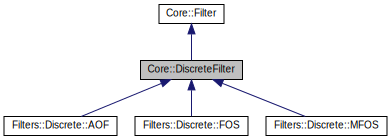
\includegraphics[width=350pt]{class_core_1_1_discrete_filter__inherit__graph}
\end{center}
\end{figure}


Граф связей класса Core\+:\+:Discrete\+Filter\+:\nopagebreak
\begin{figure}[H]
\begin{center}
\leavevmode
\includegraphics[width=190pt]{class_core_1_1_discrete_filter__coll__graph}
\end{center}
\end{figure}


\subsection{Методы}
\hypertarget{class_core_1_1_discrete_filter_a658617c64c7067bb6b98b5e9d78f982e}{}\label{class_core_1_1_discrete_filter_a658617c64c7067bb6b98b5e9d78f982e} 
\index{Core\+::\+Discrete\+Filter@{Core\+::\+Discrete\+Filter}!zero\+Iteration@{zero\+Iteration}}
\index{zero\+Iteration@{zero\+Iteration}!Core\+::\+Discrete\+Filter@{Core\+::\+Discrete\+Filter}}
\subsubsection{\texorpdfstring{zero\+Iteration()}{zeroIteration()}}
{\footnotesize\ttfamily void Core\+::\+Discrete\+Filter\+::zero\+Iteration (\begin{DoxyParamCaption}{ }\end{DoxyParamCaption})\hspace{0.3cm}{\ttfamily [override]}, {\ttfamily [protected]}, {\ttfamily [virtual]}}



Нулевая итерация алгоритма (инициализирует начальные состояния). 

Практически для всех дискретных фильтров оптимальной структуры имеет вид\+: \[Z_0 = H_0 \cdot Y_0 + e_0,\] \[H_0 = D_{00}^{xy} \cdot (D_0^y)^{-1},\] \[e_0 = m_0^x - H_0 \cdot m_0^y.\]

В гауссовском АОФ (ФНА) добавляется уравнение для апостериорной ковариации объекта\+: \[P_0 = D_0^x - H_0 \cdot (D_{00}^{xy})^T.\] 

Замещает \hyperlink{class_core_1_1_filter_af95880b734c4b8dc3d8c02f222b32506}{Core\+::\+Filter}.



Переопределяется в \hyperlink{class_filters_1_1_discrete_1_1_a_o_f_aa822fe74d7ca160f898db1c1289e17f7}{Filters\+::\+Discrete\+::\+A\+OF}.



См. определение в файле discrete\+\_\+filter.\+cc строка 21



\subsection{Данные класса}
\hypertarget{class_core_1_1_discrete_filter_a6a2d67be8eaa0df383fe080474975faa}{}\label{class_core_1_1_discrete_filter_a6a2d67be8eaa0df383fe080474975faa} 
\index{Core\+::\+Discrete\+Filter@{Core\+::\+Discrete\+Filter}!m\+\_\+task@{m\+\_\+task}}
\index{m\+\_\+task@{m\+\_\+task}!Core\+::\+Discrete\+Filter@{Core\+::\+Discrete\+Filter}}
\subsubsection{\texorpdfstring{m\+\_\+task}{m\_task}}
{\footnotesize\ttfamily \hyperlink{namespace_core_a9cd3f9b81303651b8d115031018f0ebf}{Ptr\+D\+Task} Core\+::\+Discrete\+Filter\+::m\+\_\+task\hspace{0.3cm}{\ttfamily [protected]}}

Указатель на экземпляр задачи, с которой происходит работа. 

См. определение в файле discrete\+\_\+filter.\+h строка 41



Объявления и описания членов классов находятся в файлах\+:\begin{DoxyCompactItemize}
\item 
src/core/discrete\+\_\+filter.\+h\item 
src/core/discrete\+\_\+filter.\+cc\end{DoxyCompactItemize}

\hypertarget{class_core_1_1_discrete_task}{}\section{Класс Core\+:\+:Discrete\+Task}
\label{class_core_1_1_discrete_task}\index{Core\+::\+Discrete\+Task@{Core\+::\+Discrete\+Task}}


Базовый тип задач для дискретных фильтров оптимальной структуры.  




{\ttfamily \#include \char`\"{}discrete\+\_\+task.\+h\char`\"{}}

\subsection*{Открытые члены}
\begin{DoxyCompactItemize}
\item 
\hyperlink{class_core_1_1_discrete_task_adee71fa5aa876df16d0585bdf66cd26e}{Discrete\+Task} ()\hypertarget{class_core_1_1_discrete_task_adee71fa5aa876df16d0585bdf66cd26e}{}\label{class_core_1_1_discrete_task_adee71fa5aa876df16d0585bdf66cd26e}

\begin{DoxyCompactList}\small\item\em Конструктор. \end{DoxyCompactList}\item 
virtual Vector \hyperlink{class_core_1_1_discrete_task_a49d377fa365d5ec3e05962ee751f2d9e}{a} (const Vector \&x) const =0
\begin{DoxyCompactList}\small\item\em Функция объекта $a_k(X_k) = a_k(X_k, V_k)$. \end{DoxyCompactList}\item 
virtual Vector \hyperlink{class_core_1_1_discrete_task_a82c1aa8100dd9211739f8fd9f7d52c81}{b} (const Vector \&x) const =0
\begin{DoxyCompactList}\small\item\em Функция измерителя $b(X_k) = b_k(X_k, W_k)$. \end{DoxyCompactList}\item 
virtual Vector \hyperlink{class_core_1_1_discrete_task_aed780d7286bc88d0a2debb585601b3ca}{tau} (const Vector \&m, const Matrix \&D) const =0
\begin{DoxyCompactList}\small\item\em Структурная функция прогноза $\tau_k(m, D)$. \end{DoxyCompactList}\item 
virtual Matrix \hyperlink{class_core_1_1_discrete_task_a18906155257c5febd937f2f0c633e5ed}{Theta} (const Vector \&m, const Matrix \&D) const =0
\begin{DoxyCompactList}\small\item\em Структурная функция прогноза $\Theta_k(m, D)$. \end{DoxyCompactList}\item 
virtual Vector \hyperlink{class_core_1_1_discrete_task_a09eb964bfe445c1905758bfff4fc1537}{h} (const Vector \&m, const Matrix \&D) const =0
\begin{DoxyCompactList}\small\item\em Структурная функция коррекции $h_k(m, D)$. \end{DoxyCompactList}\item 
virtual Matrix \hyperlink{class_core_1_1_discrete_task_a5fd0bac544a6e124ad071043a37881c3}{G} (const Vector \&m, const Matrix \&D) const =0
\begin{DoxyCompactList}\small\item\em Структурная функция коррекции $G_k(m, D)$. \end{DoxyCompactList}\item 
virtual Matrix \hyperlink{class_core_1_1_discrete_task_ac55ca2cd47f0c9f7e5d3d3704becee46}{F} (const Vector \&m, const Matrix \&D) const =0
\begin{DoxyCompactList}\small\item\em Структурная функция коррекции $F_k(m, D)$. \end{DoxyCompactList}\end{DoxyCompactItemize}
\subsection*{Защищенные члены}
\begin{DoxyCompactItemize}
\item 
virtual Matrix \hyperlink{class_core_1_1_discrete_task_a4fd463183eb4a6cf8fe55d0579adae47}{dadx} (const Vector \&x) const =0\hypertarget{class_core_1_1_discrete_task_a4fd463183eb4a6cf8fe55d0579adae47}{}\label{class_core_1_1_discrete_task_a4fd463183eb4a6cf8fe55d0579adae47}

\begin{DoxyCompactList}\small\item\em Вспомогательная функция, вычисляет $\nabla_x a_k(x,v)$. \end{DoxyCompactList}\item 
virtual Matrix \hyperlink{class_core_1_1_discrete_task_adcf68e112d0f30dabe00a754a4760161}{dadv} (const Vector \&x) const =0\hypertarget{class_core_1_1_discrete_task_adcf68e112d0f30dabe00a754a4760161}{}\label{class_core_1_1_discrete_task_adcf68e112d0f30dabe00a754a4760161}

\begin{DoxyCompactList}\small\item\em Вспомогательная функция, вычисляет $\nabla_v a_k(x,v)$. \end{DoxyCompactList}\item 
virtual Matrix \hyperlink{class_core_1_1_discrete_task_ac7944bf297b9fba78e35428afa05bf89}{dbdx} (const Vector \&x) const =0\hypertarget{class_core_1_1_discrete_task_ac7944bf297b9fba78e35428afa05bf89}{}\label{class_core_1_1_discrete_task_ac7944bf297b9fba78e35428afa05bf89}

\begin{DoxyCompactList}\small\item\em Вспомогательная функция, вычисляет $\nabla_x b_k(x,w)$. \end{DoxyCompactList}\item 
virtual Matrix \hyperlink{class_core_1_1_discrete_task_a6ed33be26249cbe572b55cca7614c071}{dbdw} (const Vector \&x) const =0\hypertarget{class_core_1_1_discrete_task_a6ed33be26249cbe572b55cca7614c071}{}\label{class_core_1_1_discrete_task_a6ed33be26249cbe572b55cca7614c071}

\begin{DoxyCompactList}\small\item\em Вспомогательная функция, вычисляет $\nabla_w b_k(x,w)$. \end{DoxyCompactList}\end{DoxyCompactItemize}
\subsection*{Дополнительные унаследованные члены}


\subsection{Подробное описание}
Базовый тип задач для дискретных фильтров оптимальной структуры. 

Описываемая система имеет следующий вид


\begin{DoxyItemize}
\item Объект\+: \[X_{k+1} = a_k(X_k, V_k),\ \ \ k = 0, 1, \ldots\]
\item Измеритель\+: \[Y_k = b_k(X_k, W_k),\ \ \ k = 0, 1, \ldots\]
\end{DoxyItemize}

Здесь $X_k$ -\/ вектор состояния объекта, $Y_k$ -\/ вектор измерений, $V_k, W_k$ -\/ векторы независимых дискретных белых шумов. 

См. определение в файле discrete\+\_\+task.\+h строка 23



Граф наследования\+:Core\+:\+:Discrete\+Task\+:
\nopagebreak
\begin{figure}[H]
\begin{center}
\leavevmode
\includegraphics[width=206pt]{class_core_1_1_discrete_task__inherit__graph}
\end{center}
\end{figure}


Граф связей класса Core\+:\+:Discrete\+Task\+:
\nopagebreak
\begin{figure}[H]
\begin{center}
\leavevmode
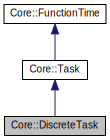
\includegraphics[width=328pt]{class_core_1_1_discrete_task__coll__graph}
\end{center}
\end{figure}


\subsection{Методы}
\index{Core\+::\+Discrete\+Task@{Core\+::\+Discrete\+Task}!a@{a}}
\index{a@{a}!Core\+::\+Discrete\+Task@{Core\+::\+Discrete\+Task}}
\subsubsection[{\texorpdfstring{a(const Vector \&x) const =0}{a(const Vector &x) const =0}}]{\setlength{\rightskip}{0pt plus 5cm}virtual Vector Core\+::\+Discrete\+Task\+::a (
\begin{DoxyParamCaption}
\item[{const Vector \&}]{x}
\end{DoxyParamCaption}
) const\hspace{0.3cm}{\ttfamily [pure virtual]}}\hypertarget{class_core_1_1_discrete_task_a49d377fa365d5ec3e05962ee751f2d9e}{}\label{class_core_1_1_discrete_task_a49d377fa365d5ec3e05962ee751f2d9e}


Функция объекта $a_k(X_k) = a_k(X_k, V_k)$. 

Шум $V_k$ генерируется внутри. 

Замещается в \hyperlink{class_tasks_1_1_discrete_1_1_landing_linear_af0c0c48603fc226055ee233f93fa21fc}{Tasks\+::\+Discrete\+::\+Landing\+Linear}.

\index{Core\+::\+Discrete\+Task@{Core\+::\+Discrete\+Task}!b@{b}}
\index{b@{b}!Core\+::\+Discrete\+Task@{Core\+::\+Discrete\+Task}}
\subsubsection[{\texorpdfstring{b(const Vector \&x) const =0}{b(const Vector &x) const =0}}]{\setlength{\rightskip}{0pt plus 5cm}virtual Vector Core\+::\+Discrete\+Task\+::b (
\begin{DoxyParamCaption}
\item[{const Vector \&}]{x}
\end{DoxyParamCaption}
) const\hspace{0.3cm}{\ttfamily [pure virtual]}}\hypertarget{class_core_1_1_discrete_task_a82c1aa8100dd9211739f8fd9f7d52c81}{}\label{class_core_1_1_discrete_task_a82c1aa8100dd9211739f8fd9f7d52c81}


Функция измерителя $b(X_k) = b_k(X_k, W_k)$. 

Шум $W_k$ генерируется внутри. 

Замещается в \hyperlink{class_tasks_1_1_discrete_1_1_landing_linear_a599d3491da6d84ba68c43433235e9980}{Tasks\+::\+Discrete\+::\+Landing\+Linear}.

\index{Core\+::\+Discrete\+Task@{Core\+::\+Discrete\+Task}!F@{F}}
\index{F@{F}!Core\+::\+Discrete\+Task@{Core\+::\+Discrete\+Task}}
\subsubsection[{\texorpdfstring{F(const Vector \&m, const Matrix \&\+D) const =0}{F(const Vector &m, const Matrix &D) const =0}}]{\setlength{\rightskip}{0pt plus 5cm}virtual Matrix Core\+::\+Discrete\+Task\+::F (
\begin{DoxyParamCaption}
\item[{const Vector \&}]{m, }
\item[{const Matrix \&}]{D}
\end{DoxyParamCaption}
) const\hspace{0.3cm}{\ttfamily [pure virtual]}}\hypertarget{class_core_1_1_discrete_task_ac55ca2cd47f0c9f7e5d3d3704becee46}{}\label{class_core_1_1_discrete_task_ac55ca2cd47f0c9f7e5d3d3704becee46}


Структурная функция коррекции $F_k(m, D)$. 

Она имеет следующий вид для


\begin{DoxyItemize}
\item гауссовского приближения\+: \[F_k(m, D) = M_N[M[b_k(m, W_k)\cdot b_k^T(m, W_k)] \ |\ m, D] - h_k(m,D) \cdot h_k^T(m, D),\]
\item линеаризованного приближения\+: \[F_k(m, D) = B_k^x(m) \cdot D \cdot B_k^{xT}(m) + B_k^w(m) \cdot D[W_k] \cdot B_k^{wT}(m).\]
\end{DoxyItemize}

Здесь $B_k^x(x) = \nabla_x b_k(x, M[W_k]),\ B_k^w(x) = \nabla_w b_k(x, M[W_k])$. 

Замещается в \hyperlink{class_tasks_1_1_discrete_1_1_landing_linear_abb4e2b054240cf909f0128721237334c}{Tasks\+::\+Discrete\+::\+Landing\+Linear}.

\index{Core\+::\+Discrete\+Task@{Core\+::\+Discrete\+Task}!G@{G}}
\index{G@{G}!Core\+::\+Discrete\+Task@{Core\+::\+Discrete\+Task}}
\subsubsection[{\texorpdfstring{G(const Vector \&m, const Matrix \&\+D) const =0}{G(const Vector &m, const Matrix &D) const =0}}]{\setlength{\rightskip}{0pt plus 5cm}virtual Matrix Core\+::\+Discrete\+Task\+::G (
\begin{DoxyParamCaption}
\item[{const Vector \&}]{m, }
\item[{const Matrix \&}]{D}
\end{DoxyParamCaption}
) const\hspace{0.3cm}{\ttfamily [pure virtual]}}\hypertarget{class_core_1_1_discrete_task_a5fd0bac544a6e124ad071043a37881c3}{}\label{class_core_1_1_discrete_task_a5fd0bac544a6e124ad071043a37881c3}


Структурная функция коррекции $G_k(m, D)$. 

Она имеет следующий вид для


\begin{DoxyItemize}
\item гауссовского приближения\+: \[G_k(m, D) = \nabla_m h_k(m,D),\]
\item линеаризованного приближения\+: \[G_k(m, D) = \nabla_m b_k(m, M[W_k]).\] 
\end{DoxyItemize}

Замещается в \hyperlink{class_tasks_1_1_discrete_1_1_landing_linear_a290890c1d3a91803249a1f5d62bc658f}{Tasks\+::\+Discrete\+::\+Landing\+Linear}.

\index{Core\+::\+Discrete\+Task@{Core\+::\+Discrete\+Task}!h@{h}}
\index{h@{h}!Core\+::\+Discrete\+Task@{Core\+::\+Discrete\+Task}}
\subsubsection[{\texorpdfstring{h(const Vector \&m, const Matrix \&\+D) const =0}{h(const Vector &m, const Matrix &D) const =0}}]{\setlength{\rightskip}{0pt plus 5cm}virtual Vector Core\+::\+Discrete\+Task\+::h (
\begin{DoxyParamCaption}
\item[{const Vector \&}]{m, }
\item[{const Matrix \&}]{D}
\end{DoxyParamCaption}
) const\hspace{0.3cm}{\ttfamily [pure virtual]}}\hypertarget{class_core_1_1_discrete_task_a09eb964bfe445c1905758bfff4fc1537}{}\label{class_core_1_1_discrete_task_a09eb964bfe445c1905758bfff4fc1537}


Структурная функция коррекции $h_k(m, D)$. 

Она имеет следующий вид для


\begin{DoxyItemize}
\item гауссовского приближения\+: \[h_k(m, D) = M_N[M[b_k(m, W_k)] \ |\ m, D],\]
\item линеаризованного приближения\+: \[h_k(m, D) = b_k(m, M[W_k]).\] 
\end{DoxyItemize}

Замещается в \hyperlink{class_tasks_1_1_discrete_1_1_landing_linear_a9b1f90547fca3b460b48693b2e16219a}{Tasks\+::\+Discrete\+::\+Landing\+Linear}.

\index{Core\+::\+Discrete\+Task@{Core\+::\+Discrete\+Task}!tau@{tau}}
\index{tau@{tau}!Core\+::\+Discrete\+Task@{Core\+::\+Discrete\+Task}}
\subsubsection[{\texorpdfstring{tau(const Vector \&m, const Matrix \&\+D) const =0}{tau(const Vector &m, const Matrix &D) const =0}}]{\setlength{\rightskip}{0pt plus 5cm}virtual Vector Core\+::\+Discrete\+Task\+::tau (
\begin{DoxyParamCaption}
\item[{const Vector \&}]{m, }
\item[{const Matrix \&}]{D}
\end{DoxyParamCaption}
) const\hspace{0.3cm}{\ttfamily [pure virtual]}}\hypertarget{class_core_1_1_discrete_task_aed780d7286bc88d0a2debb585601b3ca}{}\label{class_core_1_1_discrete_task_aed780d7286bc88d0a2debb585601b3ca}


Структурная функция прогноза $\tau_k(m, D)$. 

Она имеет следующий вид для


\begin{DoxyItemize}
\item гауссовского приближения\+: \[\tau_k(m, D) = M_N[M[a_k(m, V_k)] \ |\ m, D],\]
\item линеаризованного приближения\+: \[\tau_k(m, D) = a_k(m, M[V_k]).\] 
\end{DoxyItemize}

Замещается в \hyperlink{class_tasks_1_1_discrete_1_1_landing_linear_a8f2022967fae3dde3e7d2df3f7fa98f8}{Tasks\+::\+Discrete\+::\+Landing\+Linear}.

\index{Core\+::\+Discrete\+Task@{Core\+::\+Discrete\+Task}!Theta@{Theta}}
\index{Theta@{Theta}!Core\+::\+Discrete\+Task@{Core\+::\+Discrete\+Task}}
\subsubsection[{\texorpdfstring{Theta(const Vector \&m, const Matrix \&\+D) const =0}{Theta(const Vector &m, const Matrix &D) const =0}}]{\setlength{\rightskip}{0pt plus 5cm}virtual Matrix Core\+::\+Discrete\+Task\+::\+Theta (
\begin{DoxyParamCaption}
\item[{const Vector \&}]{m, }
\item[{const Matrix \&}]{D}
\end{DoxyParamCaption}
) const\hspace{0.3cm}{\ttfamily [pure virtual]}}\hypertarget{class_core_1_1_discrete_task_a18906155257c5febd937f2f0c633e5ed}{}\label{class_core_1_1_discrete_task_a18906155257c5febd937f2f0c633e5ed}


Структурная функция прогноза $\Theta_k(m, D)$. 

Она имеет следующий вид для


\begin{DoxyItemize}
\item гауссовского приближения\+: \[\Theta_k(m, D) = M_N[M[a_k(m, V_k)\cdot a_k^T(m, V_k)]\ |\ m, D] - \tau_k(m,D) \cdot \tau_k^T(m, D),\]
\item линеаризованного приближения\+: \[\Theta_k(m, D) = A_k^x(m) \cdot D \cdot A_k^{xT}(m) + A_k^v(m) \cdot D[V_k] \cdot A_k^{v T}(m)\]
\end{DoxyItemize}

Здесь $A_k^x(x) = \nabla_x a_k(x,M[V_k]),\ A_k^v(x) = \nabla_v a_k(x,M[V_k])$. 

Замещается в \hyperlink{class_tasks_1_1_discrete_1_1_landing_linear_a88dda707914dea5698748f445563400f}{Tasks\+::\+Discrete\+::\+Landing\+Linear}.



Объявления и описания членов классов находятся в файлах\+:\begin{DoxyCompactItemize}
\item 
src/core/discrete\+\_\+task.\+h\item 
src/core/discrete\+\_\+task.\+cc\end{DoxyCompactItemize}

\hypertarget{class_core_1_1_filter}{}\section{Класс Core\+:\+:Filter}
\label{class_core_1_1_filter}\index{Core\+::\+Filter@{Core\+::\+Filter}}


Базовый класс для всех фильтров.  




{\ttfamily \#include \char`\"{}filter.\+h\char`\"{}}

\subsection*{Открытые члены}
\begin{DoxyCompactItemize}
\item 
\hypertarget{class_core_1_1_filter_af1ac0dfc8813579e0173b315c5a3fcad}{}\label{class_core_1_1_filter_af1ac0dfc8813579e0173b315c5a3fcad} 
\hyperlink{class_core_1_1_filter_af1ac0dfc8813579e0173b315c5a3fcad}{Filter} (\hyperlink{namespace_core_a4811af8148ba137d644b9a61a042cf03}{Ptr\+Filter\+Parameters} \hyperlink{class_core_1_1_filter_a44aa749b49ba46256975ce545531ecf7}{params})
\begin{DoxyCompactList}\small\item\em Конструктор. \end{DoxyCompactList}\item 
\hypertarget{class_core_1_1_filter_a38353602e4df00367d49263dc6368268}{}\label{class_core_1_1_filter_a38353602e4df00367d49263dc6368268} 
virtual \hyperlink{class_core_1_1_filter_a38353602e4df00367d49263dc6368268}{$\sim$\+Filter} ()
\begin{DoxyCompactList}\small\item\em Деструктор. \end{DoxyCompactList}\item 
\hypertarget{class_core_1_1_filter_a76a8aef5adae9aa13ffb96e2b2398b4f}{}\label{class_core_1_1_filter_a76a8aef5adae9aa13ffb96e2b2398b4f} 
{\bfseries Filter} (const \hyperlink{class_core_1_1_filter}{Filter} \&)=delete
\item 
\hypertarget{class_core_1_1_filter_a7e05e62d95d655d1e23e4a8485baedb7}{}\label{class_core_1_1_filter_a7e05e62d95d655d1e23e4a8485baedb7} 
\hyperlink{class_core_1_1_filter}{Filter} \& {\bfseries operator=} (const \hyperlink{class_core_1_1_filter}{Filter} \&)=delete
\item 
double \hyperlink{class_core_1_1_filter_ad5070e695763edc66d211651b98c09f1}{run} ()
\begin{DoxyCompactList}\small\item\em Запускает фильтрацию. \end{DoxyCompactList}\item 
\hypertarget{class_core_1_1_filter_a40f9629b2d882f9b49745f97d98d1dd0}{}\label{class_core_1_1_filter_a40f9629b2d882f9b49745f97d98d1dd0} 
const \hyperlink{namespace_core_a60877581a235fc9566087b54d463ce9c}{Filter\+Output} \& \hyperlink{class_core_1_1_filter_a40f9629b2d882f9b49745f97d98d1dd0}{result} () const
\begin{DoxyCompactList}\small\item\em Возвращает результат работы (не имеет смысла до вызова \hyperlink{class_core_1_1_filter_ad5070e695763edc66d211651b98c09f1}{run()}). \end{DoxyCompactList}\item 
\hypertarget{class_core_1_1_filter_a44aa749b49ba46256975ce545531ecf7}{}\label{class_core_1_1_filter_a44aa749b49ba46256975ce545531ecf7} 
\hyperlink{namespace_core_a4811af8148ba137d644b9a61a042cf03}{Ptr\+Filter\+Parameters} \hyperlink{class_core_1_1_filter_a44aa749b49ba46256975ce545531ecf7}{params} ()
\begin{DoxyCompactList}\small\item\em Возвращает текущие параметры фильтра. \end{DoxyCompactList}\item 
\hypertarget{class_core_1_1_filter_a714dcb3d548dd7f0e3728f29990ff5a3}{}\label{class_core_1_1_filter_a714dcb3d548dd7f0e3728f29990ff5a3} 
\hyperlink{namespace_core_a647483da8a1266d5bbd3e9bb5cd66d08}{Ptr\+Info} \hyperlink{class_core_1_1_filter_a714dcb3d548dd7f0e3728f29990ff5a3}{info} () const
\begin{DoxyCompactList}\small\item\em Возвращает информацию о фильтре (имя, тип). \end{DoxyCompactList}\end{DoxyCompactItemize}
\subsection*{Защищенные члены}
\begin{DoxyCompactItemize}
\item 
\hypertarget{class_core_1_1_filter_ae8bb3b004400941317a1e9fdc1ca2c58}{}\label{class_core_1_1_filter_ae8bb3b004400941317a1e9fdc1ca2c58} 
virtual void \hyperlink{class_core_1_1_filter_ae8bb3b004400941317a1e9fdc1ca2c58}{init} ()
\begin{DoxyCompactList}\small\item\em Инициализирует массивы по входным данным. \end{DoxyCompactList}\item 
\hypertarget{class_core_1_1_filter_af95880b734c4b8dc3d8c02f222b32506}{}\label{class_core_1_1_filter_af95880b734c4b8dc3d8c02f222b32506} 
virtual void \hyperlink{class_core_1_1_filter_af95880b734c4b8dc3d8c02f222b32506}{zero\+Iteration} ()=0
\begin{DoxyCompactList}\small\item\em Выполняет нулевую итерацию алгоритма. \end{DoxyCompactList}\item 
\hypertarget{class_core_1_1_filter_a438681ee3e54aba2148042d9f8011ab8}{}\label{class_core_1_1_filter_a438681ee3e54aba2148042d9f8011ab8} 
virtual void \hyperlink{class_core_1_1_filter_a438681ee3e54aba2148042d9f8011ab8}{algorithm} ()=0
\begin{DoxyCompactList}\small\item\em Выполняет основной алгоритм. \end{DoxyCompactList}\item 
void \hyperlink{class_core_1_1_filter_a84c7d1ebe3931974c3beccf27f13c1c5}{write\+Result} (size\+\_\+t n, bool copy=false)
\begin{DoxyCompactList}\small\item\em Вычисляет и записывает результаты для времени $t_n$. \end{DoxyCompactList}\item 
\hypertarget{class_core_1_1_filter_a78692f8ecdfe6e2170a5d5acb0f69210}{}\label{class_core_1_1_filter_a78692f8ecdfe6e2170a5d5acb0f69210} 
void \hyperlink{class_core_1_1_filter_a78692f8ecdfe6e2170a5d5acb0f69210}{update\+Percent} (int p) const
\begin{DoxyCompactList}\small\item\em Информирует о прогрессе выполнения алгоритма (в процентах). \end{DoxyCompactList}\end{DoxyCompactItemize}
\subsection*{Защищенные данные}
\begin{DoxyCompactItemize}
\item 
\hyperlink{namespace_core_a60877581a235fc9566087b54d463ce9c}{Filter\+Output} \hyperlink{class_core_1_1_filter_a1ae638614492df7edeaa2db4f528ad65}{m\+\_\+result}
\item 
\hyperlink{namespace_core_a4811af8148ba137d644b9a61a042cf03}{Ptr\+Filter\+Parameters} \hyperlink{class_core_1_1_filter_ae4d42bb0f0e6299d4edbfc310e96d09f}{m\+\_\+params}
\item 
\hyperlink{namespace_core_a647483da8a1266d5bbd3e9bb5cd66d08}{Ptr\+Info} \hyperlink{class_core_1_1_filter_a089304c3d1695bd6b47d5bfd8fcfb574}{m\+\_\+info}
\item 
Array$<$ Vector $>$ \hyperlink{class_core_1_1_filter_abed73a8bfce99d24418f6dee90c44333}{m\+\_\+sampleX}
\item 
Array$<$ Vector $>$ \hyperlink{class_core_1_1_filter_a3e2e475b650504bb7c800e3f27364580}{m\+\_\+sampleY}
\item 
Array$<$ Vector $>$ \hyperlink{class_core_1_1_filter_af0e905e89bc5db8e07f283b68fb57a60}{m\+\_\+sampleZ}
\item 
Array$<$ Vector $>$ \hyperlink{class_core_1_1_filter_acab6dcadb8caf8f05cb2beeb1deafd74}{m\+\_\+sampleE}
\item 
\hyperlink{class_math_1_1_multivariate_normal_distribution}{Math\+::\+Multivariate\+Normal\+Distribution} \hyperlink{class_core_1_1_filter_aec144b4ca46b58af15ae602a55312996}{m\+\_\+normal\+Rand}
\end{DoxyCompactItemize}


\subsection{Подробное описание}
Базовый класс для всех фильтров. 

См. определение в файле filter.\+h строка 44



Граф наследования\+:Core\+:\+:Filter\+:
\nopagebreak
\begin{figure}[H]
\begin{center}
\leavevmode
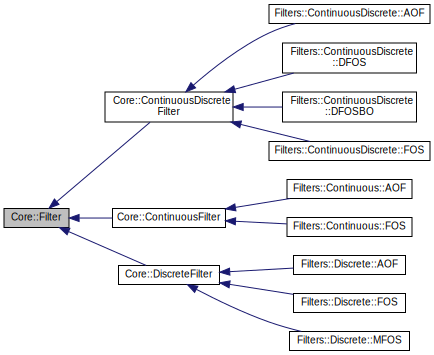
\includegraphics[width=350pt]{class_core_1_1_filter__inherit__graph}
\end{center}
\end{figure}


Граф связей класса Core\+:\+:Filter\+:
\nopagebreak
\begin{figure}[H]
\begin{center}
\leavevmode
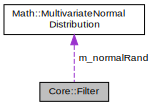
\includegraphics[width=229pt]{class_core_1_1_filter__coll__graph}
\end{center}
\end{figure}


\subsection{Методы}
\hypertarget{class_core_1_1_filter_ad5070e695763edc66d211651b98c09f1}{}\label{class_core_1_1_filter_ad5070e695763edc66d211651b98c09f1} 
\index{Core\+::\+Filter@{Core\+::\+Filter}!run@{run}}
\index{run@{run}!Core\+::\+Filter@{Core\+::\+Filter}}
\subsubsection{\texorpdfstring{run()}{run()}}
{\footnotesize\ttfamily double Core\+::\+Filter\+::run (\begin{DoxyParamCaption}{ }\end{DoxyParamCaption})}



Запускает фильтрацию. 

\begin{DoxyReturn}{Возвращает}
полное время работы.
\end{DoxyReturn}
Схематически, полный цикл работы фильтра выглядит так\+: 
\begin{DoxyCode}
\hyperlink{class_core_1_1_filter_ae8bb3b004400941317a1e9fdc1ca2c58}{init}();
\hyperlink{class_core_1_1_filter_af95880b734c4b8dc3d8c02f222b32506}{zeroIteration}();
\hyperlink{class_core_1_1_filter_a438681ee3e54aba2148042d9f8011ab8}{algorithm}();
\end{DoxyCode}
 

См. определение в файле filter.\+cc строка 28

\hypertarget{class_core_1_1_filter_a84c7d1ebe3931974c3beccf27f13c1c5}{}\label{class_core_1_1_filter_a84c7d1ebe3931974c3beccf27f13c1c5} 
\index{Core\+::\+Filter@{Core\+::\+Filter}!write\+Result@{write\+Result}}
\index{write\+Result@{write\+Result}!Core\+::\+Filter@{Core\+::\+Filter}}
\subsubsection{\texorpdfstring{write\+Result()}{writeResult()}}
{\footnotesize\ttfamily void Core\+::\+Filter\+::write\+Result (\begin{DoxyParamCaption}\item[{size\+\_\+t}]{n,  }\item[{bool}]{copy = {\ttfamily false} }\end{DoxyParamCaption})\hspace{0.3cm}{\ttfamily [protected]}}



Вычисляет и записывает результаты для времени $t_n$. 


\begin{DoxyParams}{Аргументы}
{\em n} & -\/ результат записывается в ячейку с этим индексом. \\
\hline
{\em copy} & -\/ если false (по-\/умолчанию), то вычисляются все характеристики, если true, то только характеристики для $x_{t_n}$, остальные копируются из предыдущей ячейки (опция для дискретных фильтров -\/ \char`\"{}порожки\char`\"{} на графиках). \\
\hline
\end{DoxyParams}


См. определение в файле filter.\+cc строка 66



\subsection{Данные класса}
\hypertarget{class_core_1_1_filter_a089304c3d1695bd6b47d5bfd8fcfb574}{}\label{class_core_1_1_filter_a089304c3d1695bd6b47d5bfd8fcfb574} 
\index{Core\+::\+Filter@{Core\+::\+Filter}!m\+\_\+info@{m\+\_\+info}}
\index{m\+\_\+info@{m\+\_\+info}!Core\+::\+Filter@{Core\+::\+Filter}}
\subsubsection{\texorpdfstring{m\+\_\+info}{m\_info}}
{\footnotesize\ttfamily \hyperlink{namespace_core_a647483da8a1266d5bbd3e9bb5cd66d08}{Ptr\+Info} Core\+::\+Filter\+::m\+\_\+info\hspace{0.3cm}{\ttfamily [protected]}}

Информация (имя, тип). 

См. определение в файле filter.\+h строка 114

\hypertarget{class_core_1_1_filter_aec144b4ca46b58af15ae602a55312996}{}\label{class_core_1_1_filter_aec144b4ca46b58af15ae602a55312996} 
\index{Core\+::\+Filter@{Core\+::\+Filter}!m\+\_\+normal\+Rand@{m\+\_\+normal\+Rand}}
\index{m\+\_\+normal\+Rand@{m\+\_\+normal\+Rand}!Core\+::\+Filter@{Core\+::\+Filter}}
\subsubsection{\texorpdfstring{m\+\_\+normal\+Rand}{m\_normalRand}}
{\footnotesize\ttfamily \hyperlink{class_math_1_1_multivariate_normal_distribution}{Math\+::\+Multivariate\+Normal\+Distribution} Core\+::\+Filter\+::m\+\_\+normal\+Rand\hspace{0.3cm}{\ttfamily [protected]}}

Генератор гауссовских случайных векторов. 

См. определение в файле filter.\+h строка 121

\hypertarget{class_core_1_1_filter_ae4d42bb0f0e6299d4edbfc310e96d09f}{}\label{class_core_1_1_filter_ae4d42bb0f0e6299d4edbfc310e96d09f} 
\index{Core\+::\+Filter@{Core\+::\+Filter}!m\+\_\+params@{m\+\_\+params}}
\index{m\+\_\+params@{m\+\_\+params}!Core\+::\+Filter@{Core\+::\+Filter}}
\subsubsection{\texorpdfstring{m\+\_\+params}{m\_params}}
{\footnotesize\ttfamily \hyperlink{namespace_core_a4811af8148ba137d644b9a61a042cf03}{Ptr\+Filter\+Parameters} Core\+::\+Filter\+::m\+\_\+params\hspace{0.3cm}{\ttfamily [protected]}}

Параметры. 

См. определение в файле filter.\+h строка 113

\hypertarget{class_core_1_1_filter_a1ae638614492df7edeaa2db4f528ad65}{}\label{class_core_1_1_filter_a1ae638614492df7edeaa2db4f528ad65} 
\index{Core\+::\+Filter@{Core\+::\+Filter}!m\+\_\+result@{m\+\_\+result}}
\index{m\+\_\+result@{m\+\_\+result}!Core\+::\+Filter@{Core\+::\+Filter}}
\subsubsection{\texorpdfstring{m\+\_\+result}{m\_result}}
{\footnotesize\ttfamily \hyperlink{namespace_core_a60877581a235fc9566087b54d463ce9c}{Filter\+Output} Core\+::\+Filter\+::m\+\_\+result\hspace{0.3cm}{\ttfamily [protected]}}

Результаты работы. 

См. определение в файле filter.\+h строка 112

\hypertarget{class_core_1_1_filter_acab6dcadb8caf8f05cb2beeb1deafd74}{}\label{class_core_1_1_filter_acab6dcadb8caf8f05cb2beeb1deafd74} 
\index{Core\+::\+Filter@{Core\+::\+Filter}!m\+\_\+sampleE@{m\+\_\+sampleE}}
\index{m\+\_\+sampleE@{m\+\_\+sampleE}!Core\+::\+Filter@{Core\+::\+Filter}}
\subsubsection{\texorpdfstring{m\+\_\+sampleE}{m\_sampleE}}
{\footnotesize\ttfamily Array$<$Vector$>$ Core\+::\+Filter\+::m\+\_\+sampleE\hspace{0.3cm}{\ttfamily [protected]}}

Массив под выборку $E$. 

См. определение в файле filter.\+h строка 119

\hypertarget{class_core_1_1_filter_abed73a8bfce99d24418f6dee90c44333}{}\label{class_core_1_1_filter_abed73a8bfce99d24418f6dee90c44333} 
\index{Core\+::\+Filter@{Core\+::\+Filter}!m\+\_\+sampleX@{m\+\_\+sampleX}}
\index{m\+\_\+sampleX@{m\+\_\+sampleX}!Core\+::\+Filter@{Core\+::\+Filter}}
\subsubsection{\texorpdfstring{m\+\_\+sampleX}{m\_sampleX}}
{\footnotesize\ttfamily Array$<$Vector$>$ Core\+::\+Filter\+::m\+\_\+sampleX\hspace{0.3cm}{\ttfamily [protected]}}

Массив под выборку $X$. 

См. определение в файле filter.\+h строка 116

\hypertarget{class_core_1_1_filter_a3e2e475b650504bb7c800e3f27364580}{}\label{class_core_1_1_filter_a3e2e475b650504bb7c800e3f27364580} 
\index{Core\+::\+Filter@{Core\+::\+Filter}!m\+\_\+sampleY@{m\+\_\+sampleY}}
\index{m\+\_\+sampleY@{m\+\_\+sampleY}!Core\+::\+Filter@{Core\+::\+Filter}}
\subsubsection{\texorpdfstring{m\+\_\+sampleY}{m\_sampleY}}
{\footnotesize\ttfamily Array$<$Vector$>$ Core\+::\+Filter\+::m\+\_\+sampleY\hspace{0.3cm}{\ttfamily [protected]}}

Массив под выборку $Y$. 

См. определение в файле filter.\+h строка 117

\hypertarget{class_core_1_1_filter_af0e905e89bc5db8e07f283b68fb57a60}{}\label{class_core_1_1_filter_af0e905e89bc5db8e07f283b68fb57a60} 
\index{Core\+::\+Filter@{Core\+::\+Filter}!m\+\_\+sampleZ@{m\+\_\+sampleZ}}
\index{m\+\_\+sampleZ@{m\+\_\+sampleZ}!Core\+::\+Filter@{Core\+::\+Filter}}
\subsubsection{\texorpdfstring{m\+\_\+sampleZ}{m\_sampleZ}}
{\footnotesize\ttfamily Array$<$Vector$>$ Core\+::\+Filter\+::m\+\_\+sampleZ\hspace{0.3cm}{\ttfamily [protected]}}

Массив под выборку $Z$. 

См. определение в файле filter.\+h строка 118



Объявления и описания членов классов находятся в файлах\+:\begin{DoxyCompactItemize}
\item 
src/core/filter.\+h\item 
src/core/filter.\+cc\end{DoxyCompactItemize}

\hypertarget{class_filters_1_1_filter_factory}{}\section{Класс Filters\+:\+:Filter\+Factory}
\label{class_filters_1_1_filter_factory}\index{Filters\+::\+Filter\+Factory@{Filters\+::\+Filter\+Factory}}


Фабричный класс для создания экземпляров классов фильтров.  




{\ttfamily \#include \char`\"{}filters\+\_\+factory.\+h\char`\"{}}

\subsection*{Открытые статические члены}
\begin{DoxyCompactItemize}
\item 
static \hyperlink{namespace_core_afba80c2cb714c7d5793d9bcb9591e156}{Core\+::\+Ptr\+Filter} \hyperlink{class_filters_1_1_filter_factory_a404c33c0459c3997d4ad7d488580f404}{create} (\hyperlink{namespace_core_af88278693f3c866f217da796f4bb9af7}{Core\+::\+F\+I\+L\+T\+E\+R\+\_\+\+T\+Y\+PE} type, \hyperlink{namespace_filters_a1b615faac44ef992d0af44da40ff26d7}{F\+I\+L\+T\+E\+R\+\_\+\+ID} id, \hyperlink{namespace_core_a4811af8148ba137d644b9a61a042cf03}{Core\+::\+Ptr\+Filter\+Parameters} params, \hyperlink{namespace_core_abfda8f69fcacfcea2696549b548ed737}{Core\+::\+Ptr\+Task} task)
\begin{DoxyCompactList}\small\item\em Создает экземпляр фильтра по входным параметрам. \end{DoxyCompactList}\end{DoxyCompactItemize}
\subsection*{Закрытые статические члены}
\begin{DoxyCompactItemize}
\item 
\hypertarget{class_filters_1_1_filter_factory_a0c5ef077dc893e280e0fe63a42d7d84f}{}\label{class_filters_1_1_filter_factory_a0c5ef077dc893e280e0fe63a42d7d84f} 
static \hyperlink{namespace_core_afba80c2cb714c7d5793d9bcb9591e156}{Core\+::\+Ptr\+Filter} \hyperlink{class_filters_1_1_filter_factory_a0c5ef077dc893e280e0fe63a42d7d84f}{create\+Continuous} (\hyperlink{namespace_filters_a1b615faac44ef992d0af44da40ff26d7}{F\+I\+L\+T\+E\+R\+\_\+\+ID} id, \hyperlink{namespace_core_a4811af8148ba137d644b9a61a042cf03}{Core\+::\+Ptr\+Filter\+Parameters} params, \hyperlink{namespace_core_abfda8f69fcacfcea2696549b548ed737}{Core\+::\+Ptr\+Task} task)
\begin{DoxyCompactList}\small\item\em Вспомогательный метод для создания непрерывных фильтров оптимальной структуры. \end{DoxyCompactList}\item 
\hypertarget{class_filters_1_1_filter_factory_a0db9538bb9f4cf762c382a9a264d67d9}{}\label{class_filters_1_1_filter_factory_a0db9538bb9f4cf762c382a9a264d67d9} 
static \hyperlink{namespace_core_afba80c2cb714c7d5793d9bcb9591e156}{Core\+::\+Ptr\+Filter} \hyperlink{class_filters_1_1_filter_factory_a0db9538bb9f4cf762c382a9a264d67d9}{create\+Continuous\+Discrete} (\hyperlink{namespace_filters_a1b615faac44ef992d0af44da40ff26d7}{F\+I\+L\+T\+E\+R\+\_\+\+ID} id, \hyperlink{namespace_core_a4811af8148ba137d644b9a61a042cf03}{Core\+::\+Ptr\+Filter\+Parameters} params, \hyperlink{namespace_core_abfda8f69fcacfcea2696549b548ed737}{Core\+::\+Ptr\+Task} task)
\begin{DoxyCompactList}\small\item\em Вспомогательный метод для создания непрерывно-\/дискретных фильтров оптимальной структуры. \end{DoxyCompactList}\item 
\hypertarget{class_filters_1_1_filter_factory_a2afeb17c3cb614d3319feac10ccdcfa9}{}\label{class_filters_1_1_filter_factory_a2afeb17c3cb614d3319feac10ccdcfa9} 
static \hyperlink{namespace_core_afba80c2cb714c7d5793d9bcb9591e156}{Core\+::\+Ptr\+Filter} \hyperlink{class_filters_1_1_filter_factory_a2afeb17c3cb614d3319feac10ccdcfa9}{create\+Discrete} (\hyperlink{namespace_filters_a1b615faac44ef992d0af44da40ff26d7}{F\+I\+L\+T\+E\+R\+\_\+\+ID} id, \hyperlink{namespace_core_a4811af8148ba137d644b9a61a042cf03}{Core\+::\+Ptr\+Filter\+Parameters} params, \hyperlink{namespace_core_abfda8f69fcacfcea2696549b548ed737}{Core\+::\+Ptr\+Task} task)
\begin{DoxyCompactList}\small\item\em Вспомогательный метод для создания дискретных фильтров оптимальной структуры. \end{DoxyCompactList}\end{DoxyCompactItemize}


\subsection{Подробное описание}
Фабричный класс для создания экземпляров классов фильтров. 

См. определение в файле filters\+\_\+factory.\+h строка 35



\subsection{Методы}
\hypertarget{class_filters_1_1_filter_factory_a404c33c0459c3997d4ad7d488580f404}{}\label{class_filters_1_1_filter_factory_a404c33c0459c3997d4ad7d488580f404} 
\index{Filters\+::\+Filter\+Factory@{Filters\+::\+Filter\+Factory}!create@{create}}
\index{create@{create}!Filters\+::\+Filter\+Factory@{Filters\+::\+Filter\+Factory}}
\subsubsection{\texorpdfstring{create()}{create()}}
{\footnotesize\ttfamily \hyperlink{namespace_core_afba80c2cb714c7d5793d9bcb9591e156}{Ptr\+Filter} Filters\+::\+Filter\+Factory\+::create (\begin{DoxyParamCaption}\item[{\hyperlink{namespace_core_af88278693f3c866f217da796f4bb9af7}{Core\+::\+F\+I\+L\+T\+E\+R\+\_\+\+T\+Y\+PE}}]{type,  }\item[{\hyperlink{namespace_filters_a1b615faac44ef992d0af44da40ff26d7}{F\+I\+L\+T\+E\+R\+\_\+\+ID}}]{id,  }\item[{\hyperlink{namespace_core_a4811af8148ba137d644b9a61a042cf03}{Core\+::\+Ptr\+Filter\+Parameters}}]{params,  }\item[{\hyperlink{namespace_core_abfda8f69fcacfcea2696549b548ed737}{Core\+::\+Ptr\+Task}}]{task }\end{DoxyParamCaption})\hspace{0.3cm}{\ttfamily [static]}}



Создает экземпляр фильтра по входным параметрам. 


\begin{DoxyParams}{Аргументы}
{\em type} & -\/ тип фильтра (непрерывный, дискретный, ...). \\
\hline
{\em id} & -\/ идентификатор фильтра (АОФ, ФМП и т.\+д.). \\
\hline
{\em params} & -\/ указатель на параметры, которые будет использовать фильтр. \\
\hline
{\em task} & -\/ указатель на экземпляр решаемой задачи \\
\hline
\end{DoxyParams}
\begin{DoxyReturn}{Возвращает}
указатель на созданный экземпляр фильтра. 
\end{DoxyReturn}


См. определение в файле filters\+\_\+factory.\+cc строка 10



Объявления и описания членов классов находятся в файлах\+:\begin{DoxyCompactItemize}
\item 
src/filters/filters\+\_\+factory.\+h\item 
src/filters/filters\+\_\+factory.\+cc\end{DoxyCompactItemize}

\hypertarget{class_core_1_1_filter_parameters}{}\section{Класс Core\+:\+:Filter\+Parameters}
\label{class_core_1_1_filter_parameters}\index{Core\+::\+Filter\+Parameters@{Core\+::\+Filter\+Parameters}}


Класс для работы с параметрами фильтра.  




{\ttfamily \#include \char`\"{}filter\+\_\+parameters.\+h\char`\"{}}

\subsection*{Открытые члены}
\begin{DoxyCompactItemize}
\item 
\hyperlink{class_core_1_1_filter_parameters_aac0d147953f2293a426cd25e031016f2}{Filter\+Parameters} (double \hyperlink{class_core_1_1_filter_parameters_a7f0a5aee70070bede068818c381d2b41}{max\+Time}, double \hyperlink{class_core_1_1_filter_parameters_a749a4ecbb2bbd3463c340232097010b9}{measurement\+Step}, double \hyperlink{class_core_1_1_filter_parameters_ae4adb72b26c25f38673e0a573b1e3a36}{prediction\+Step}, double \hyperlink{class_core_1_1_filter_parameters_aeb2ccbc82692341b2831aeea8a96dcfd}{integration\+Step}, ulong \hyperlink{class_core_1_1_filter_parameters_a879401aa0aa48b363fd35b3d85eced43}{sample\+Size}, ulong \hyperlink{class_core_1_1_filter_parameters_a4294f7904cbaaac16768cbb8c2a9e40c}{order\+Mult}=1)
\begin{DoxyCompactList}\small\item\em Конструктор. \end{DoxyCompactList}\item 
const double \& \hyperlink{class_core_1_1_filter_parameters_a7f0a5aee70070bede068818c381d2b41}{max\+Time} () const \hypertarget{class_core_1_1_filter_parameters_a7f0a5aee70070bede068818c381d2b41}{}\label{class_core_1_1_filter_parameters_a7f0a5aee70070bede068818c381d2b41}

\begin{DoxyCompactList}\small\item\em Возвращает время $T_{max}$ окончания фильтрации. \end{DoxyCompactList}\item 
const double \& \hyperlink{class_core_1_1_filter_parameters_a749a4ecbb2bbd3463c340232097010b9}{measurement\+Step} () const \hypertarget{class_core_1_1_filter_parameters_a749a4ecbb2bbd3463c340232097010b9}{}\label{class_core_1_1_filter_parameters_a749a4ecbb2bbd3463c340232097010b9}

\begin{DoxyCompactList}\small\item\em Возвращает интервал $\delta t$ между измерениями. \end{DoxyCompactList}\item 
const double \& \hyperlink{class_core_1_1_filter_parameters_ae4adb72b26c25f38673e0a573b1e3a36}{prediction\+Step} () const \hypertarget{class_core_1_1_filter_parameters_ae4adb72b26c25f38673e0a573b1e3a36}{}\label{class_core_1_1_filter_parameters_ae4adb72b26c25f38673e0a573b1e3a36}

\begin{DoxyCompactList}\small\item\em Возвращает интервал $\delta \tau$ между прогнозами. \end{DoxyCompactList}\item 
const double \& \hyperlink{class_core_1_1_filter_parameters_aeb2ccbc82692341b2831aeea8a96dcfd}{integration\+Step} () const \hypertarget{class_core_1_1_filter_parameters_aeb2ccbc82692341b2831aeea8a96dcfd}{}\label{class_core_1_1_filter_parameters_aeb2ccbc82692341b2831aeea8a96dcfd}

\begin{DoxyCompactList}\small\item\em Возвращает шаг интегрирования $\Delta t$. \end{DoxyCompactList}\item 
const ulong \& \hyperlink{class_core_1_1_filter_parameters_ace491a0120f53d874ee20fbce9e30735}{measurement\+Count} () const \hypertarget{class_core_1_1_filter_parameters_ace491a0120f53d874ee20fbce9e30735}{}\label{class_core_1_1_filter_parameters_ace491a0120f53d874ee20fbce9e30735}

\begin{DoxyCompactList}\small\item\em Возвращает количество $K$ измерений. \end{DoxyCompactList}\item 
const ulong \& \hyperlink{class_core_1_1_filter_parameters_afee5fdf7c715c7e10f776581382f6f43}{prediction\+Count} () const \hypertarget{class_core_1_1_filter_parameters_afee5fdf7c715c7e10f776581382f6f43}{}\label{class_core_1_1_filter_parameters_afee5fdf7c715c7e10f776581382f6f43}

\begin{DoxyCompactList}\small\item\em Возвращает количество $L$ прогнозов между двумя измерениями. \end{DoxyCompactList}\item 
const ulong \& \hyperlink{class_core_1_1_filter_parameters_af1e572c3791e4501f85fdfde72c2e198}{integration\+Count} () const \hypertarget{class_core_1_1_filter_parameters_af1e572c3791e4501f85fdfde72c2e198}{}\label{class_core_1_1_filter_parameters_af1e572c3791e4501f85fdfde72c2e198}

\begin{DoxyCompactList}\small\item\em Возвращает количество $N$ интегрирований между двумя прогнозами. \end{DoxyCompactList}\item 
const ulong \& \hyperlink{class_core_1_1_filter_parameters_a879401aa0aa48b363fd35b3d85eced43}{sample\+Size} () const \hypertarget{class_core_1_1_filter_parameters_a879401aa0aa48b363fd35b3d85eced43}{}\label{class_core_1_1_filter_parameters_a879401aa0aa48b363fd35b3d85eced43}

\begin{DoxyCompactList}\small\item\em Возвращает размер выборок. \end{DoxyCompactList}\item 
const ulong \& \hyperlink{class_core_1_1_filter_parameters_a4294f7904cbaaac16768cbb8c2a9e40c}{order\+Mult} () const \hypertarget{class_core_1_1_filter_parameters_a4294f7904cbaaac16768cbb8c2a9e40c}{}\label{class_core_1_1_filter_parameters_a4294f7904cbaaac16768cbb8c2a9e40c}

\begin{DoxyCompactList}\small\item\em Возвращает кратность порядка фильтра для ФКП (ФОСпп). \end{DoxyCompactList}\item 
void \hyperlink{class_core_1_1_filter_parameters_a649fb04817a251986e9bffb264b3a22a}{set\+Max\+Time} (double tmax)\hypertarget{class_core_1_1_filter_parameters_a649fb04817a251986e9bffb264b3a22a}{}\label{class_core_1_1_filter_parameters_a649fb04817a251986e9bffb264b3a22a}

\begin{DoxyCompactList}\small\item\em Устанавливает время $T_{max}$ окончания фильтрации. \end{DoxyCompactList}\item 
void \hyperlink{class_core_1_1_filter_parameters_a53a29d979978514b85078f3d7263c947}{set\+Measurement\+Step} (double step)\hypertarget{class_core_1_1_filter_parameters_a53a29d979978514b85078f3d7263c947}{}\label{class_core_1_1_filter_parameters_a53a29d979978514b85078f3d7263c947}

\begin{DoxyCompactList}\small\item\em Устанавливает интервал $\delta t$ между измерениями. \end{DoxyCompactList}\item 
void \hyperlink{class_core_1_1_filter_parameters_abc28925f9ee2213da37a000dc761cb05}{set\+Prediction\+Step} (double step)\hypertarget{class_core_1_1_filter_parameters_abc28925f9ee2213da37a000dc761cb05}{}\label{class_core_1_1_filter_parameters_abc28925f9ee2213da37a000dc761cb05}

\begin{DoxyCompactList}\small\item\em Устанавливает интервал $\delta \tau$ между прогнозами. \end{DoxyCompactList}\item 
void \hyperlink{class_core_1_1_filter_parameters_a8349d4d94febddd3367865b60b3deed5}{set\+Integration\+Step} (double step)\hypertarget{class_core_1_1_filter_parameters_a8349d4d94febddd3367865b60b3deed5}{}\label{class_core_1_1_filter_parameters_a8349d4d94febddd3367865b60b3deed5}

\begin{DoxyCompactList}\small\item\em Устанавливает шаг интегрирования $\Delta t$. \end{DoxyCompactList}\item 
void \hyperlink{class_core_1_1_filter_parameters_a3b7b8345d450d60f8e4fbe7bbe825fd6}{set\+Sample\+Size} (ulong size)\hypertarget{class_core_1_1_filter_parameters_a3b7b8345d450d60f8e4fbe7bbe825fd6}{}\label{class_core_1_1_filter_parameters_a3b7b8345d450d60f8e4fbe7bbe825fd6}

\begin{DoxyCompactList}\small\item\em Устанавливает размер выборок. \end{DoxyCompactList}\item 
void \hyperlink{class_core_1_1_filter_parameters_a763a74eb5ae44bfde79110a38bb79867}{set\+Order\+Mult} (ulong order)\hypertarget{class_core_1_1_filter_parameters_a763a74eb5ae44bfde79110a38bb79867}{}\label{class_core_1_1_filter_parameters_a763a74eb5ae44bfde79110a38bb79867}

\begin{DoxyCompactList}\small\item\em Устанавливает кратность порядка фильтра для ФКП (ФОСпп). \end{DoxyCompactList}\end{DoxyCompactItemize}
\subsection*{Закрытые члены}
\begin{DoxyCompactItemize}
\item 
void \hyperlink{class_core_1_1_filter_parameters_abd97b1d6389fb381e9808f15a271dfc3}{correct\+Step\+And\+Count} (const double \&interval\+Length, double \&step, ulong \&count)
\begin{DoxyCompactList}\small\item\em Корректирует величину шага и количество шагов в данном интервале. \end{DoxyCompactList}\end{DoxyCompactItemize}
\subsection*{Закрытые данные}
\begin{DoxyCompactItemize}
\item 
double \hyperlink{class_core_1_1_filter_parameters_a5f906190ee024f4df75f8279e9986f2c}{m\+\_\+max\+Time}
\item 
double \hyperlink{class_core_1_1_filter_parameters_a68b0fe638b3a00a16cfa07f7d6a229fb}{m\+\_\+measurement\+Step}
\item 
double \hyperlink{class_core_1_1_filter_parameters_a1d15be069d981b8f7e1252cb0fd8970d}{m\+\_\+prediction\+Step}
\item 
double \hyperlink{class_core_1_1_filter_parameters_ab63c375a5b76a516da339b058af687ae}{m\+\_\+integration\+Step}
\item 
ulong \hyperlink{class_core_1_1_filter_parameters_a931e9e09796c055d6c28d7c93d3121d9}{m\+\_\+measurement\+Count}
\item 
ulong \hyperlink{class_core_1_1_filter_parameters_a6b692ee25b7554649a81c073c009855a}{m\+\_\+prediction\+Count}
\item 
ulong \hyperlink{class_core_1_1_filter_parameters_af28ca1d6c952ad42a5dfbeb6a7e916e5}{m\+\_\+integration\+Count}
\item 
ulong \hyperlink{class_core_1_1_filter_parameters_a70abc1052c13fe0fb7f971229d7a1316}{m\+\_\+sample\+Size}
\item 
ulong \hyperlink{class_core_1_1_filter_parameters_abbf3de6b71f358870d750c829d1ef4ea}{m\+\_\+order\+Mult}
\end{DoxyCompactItemize}


\subsection{Подробное описание}
Класс для работы с параметрами фильтра. 

Основное внимание уделено обработке временных интервалов.

Пусть отрезок времени $t$, обрабатываемого фильтром, равен $[0, T_{max}]$.

На этом отрезке времени производятся измерения с шагом $\delta t$.

Между измерениями (в фильтрах с дискретными прогнозами) осуществляется прогнозирование. Интервал между прогнозами $\delta \tau$.

Шаг интегрирования системы $\Delta t$.

Эти величины корректируются (при изменении) так, чтобы количество интегрирований $N$ между соседними прогнозами, количество прогнозов $L$ между соседними измерениями и количесвтво измерений $K$ на всём временном интервале были целыми числами.

То есть $\Delta t, \delta \tau, \delta t$ и $T_{max}$ немного подкручиваются так, что выражения ниже становятся корректными (в смысле делимости нацело) в совокупности\+:

\[K = \frac{T_{max}}{\delta t};\ \ \ L = \frac{\delta t}{\delta \tau};\ \ \ N = \frac{\delta \tau}{\Delta t}\] 

См. определение в файле filter\+\_\+parameters.\+h строка 38



\subsection{Конструктор(ы)}
\index{Core\+::\+Filter\+Parameters@{Core\+::\+Filter\+Parameters}!Filter\+Parameters@{Filter\+Parameters}}
\index{Filter\+Parameters@{Filter\+Parameters}!Core\+::\+Filter\+Parameters@{Core\+::\+Filter\+Parameters}}
\subsubsection[{\texorpdfstring{Filter\+Parameters(double max\+Time, double measurement\+Step, double prediction\+Step, double integration\+Step, ulong sample\+Size, ulong order\+Mult=1)}{FilterParameters(double maxTime, double measurementStep, double predictionStep, double integrationStep, ulong sampleSize, ulong orderMult=1)}}]{\setlength{\rightskip}{0pt plus 5cm}Core\+::\+Filter\+Parameters\+::\+Filter\+Parameters (
\begin{DoxyParamCaption}
\item[{double}]{max\+Time, }
\item[{double}]{measurement\+Step, }
\item[{double}]{prediction\+Step, }
\item[{double}]{integration\+Step, }
\item[{ulong}]{sample\+Size, }
\item[{ulong}]{order\+Mult = {\ttfamily 1}}
\end{DoxyParamCaption}
)}\hypertarget{class_core_1_1_filter_parameters_aac0d147953f2293a426cd25e031016f2}{}\label{class_core_1_1_filter_parameters_aac0d147953f2293a426cd25e031016f2}


Конструктор. 


\begin{DoxyParams}{Аргументы}
{\em max\+Time} & -\/ время $T_{max}$ окончания фильтрации. \\
\hline
{\em measurement\+Step} & -\/ интервал $\delta t$ между измерениями. \\
\hline
{\em prediction\+Step} & -\/ интервал $\delta \tau$ между (дискретными) прогнозами. \\
\hline
{\em integration\+Step} & -\/ шаг интегрирования $\Delta t$. \\
\hline
{\em sample\+Size} & -\/ размер выборок. \\
\hline
{\em order\+Mult} & -\/ кратность порядка фильтра для ФКП (ФОСпп).\\
\hline
\end{DoxyParams}
После автоматической коррекции значения могут несколько отличаться от заданных. 

См. определение в файле filter\+\_\+parameters.\+cc строка 8



\subsection{Методы}
\index{Core\+::\+Filter\+Parameters@{Core\+::\+Filter\+Parameters}!correct\+Step\+And\+Count@{correct\+Step\+And\+Count}}
\index{correct\+Step\+And\+Count@{correct\+Step\+And\+Count}!Core\+::\+Filter\+Parameters@{Core\+::\+Filter\+Parameters}}
\subsubsection[{\texorpdfstring{correct\+Step\+And\+Count(const double \&interval\+Length, double \&step, ulong \&count)}{correctStepAndCount(const double &intervalLength, double &step, ulong &count)}}]{\setlength{\rightskip}{0pt plus 5cm}void Core\+::\+Filter\+Parameters\+::correct\+Step\+And\+Count (
\begin{DoxyParamCaption}
\item[{const double \&}]{interval\+Length, }
\item[{double \&}]{step, }
\item[{ulong \&}]{count}
\end{DoxyParamCaption}
)\hspace{0.3cm}{\ttfamily [private]}}\hypertarget{class_core_1_1_filter_parameters_abd97b1d6389fb381e9808f15a271dfc3}{}\label{class_core_1_1_filter_parameters_abd97b1d6389fb381e9808f15a271dfc3}


Корректирует величину шага и количество шагов в данном интервале. 


\begin{DoxyParams}[1]{Аргументы}
\mbox{\tt in}  & {\em interval\+Length} & -\/ длина $d$ интервала. \\
\hline
\mbox{\tt in,out}  & {\em step} & -\/ шаг $h$ (корректируется, если необходимо). \\
\hline
\mbox{\tt out}  & {\em count} & -\/ количиство $N$ шагов $h$, укладывающихся в $d$ (вычисляется).\\
\hline
\end{DoxyParams}
Корректировка работает следующим образом\+:

Сначала вычисляется целое число $N' = \frac{d}{h}$ (дробная часть отбрасывается).

Если $\frac{d}{h} - N' >= \frac{1}{2}$, то $N = N' + 1$, иначе $N = N'$.

Теперь корректируется шаг\+: $h = \frac{d}{N}$. 

См. определение в файле filter\+\_\+parameters.\+cc строка 117



\subsection{Данные класса}
\index{Core\+::\+Filter\+Parameters@{Core\+::\+Filter\+Parameters}!m\+\_\+integration\+Count@{m\+\_\+integration\+Count}}
\index{m\+\_\+integration\+Count@{m\+\_\+integration\+Count}!Core\+::\+Filter\+Parameters@{Core\+::\+Filter\+Parameters}}
\subsubsection[{\texorpdfstring{m\+\_\+integration\+Count}{m_integrationCount}}]{\setlength{\rightskip}{0pt plus 5cm}ulong Core\+::\+Filter\+Parameters\+::m\+\_\+integration\+Count\hspace{0.3cm}{\ttfamily [private]}}\hypertarget{class_core_1_1_filter_parameters_af28ca1d6c952ad42a5dfbeb6a7e916e5}{}\label{class_core_1_1_filter_parameters_af28ca1d6c952ad42a5dfbeb6a7e916e5}
Количество $N$ интегрирований между двумя прогнозами. 

См. определение в файле filter\+\_\+parameters.\+h строка 130

\index{Core\+::\+Filter\+Parameters@{Core\+::\+Filter\+Parameters}!m\+\_\+integration\+Step@{m\+\_\+integration\+Step}}
\index{m\+\_\+integration\+Step@{m\+\_\+integration\+Step}!Core\+::\+Filter\+Parameters@{Core\+::\+Filter\+Parameters}}
\subsubsection[{\texorpdfstring{m\+\_\+integration\+Step}{m_integrationStep}}]{\setlength{\rightskip}{0pt plus 5cm}double Core\+::\+Filter\+Parameters\+::m\+\_\+integration\+Step\hspace{0.3cm}{\ttfamily [private]}}\hypertarget{class_core_1_1_filter_parameters_ab63c375a5b76a516da339b058af687ae}{}\label{class_core_1_1_filter_parameters_ab63c375a5b76a516da339b058af687ae}
Шаг интегрирования $\Delta t$. 

См. определение в файле filter\+\_\+parameters.\+h строка 126

\index{Core\+::\+Filter\+Parameters@{Core\+::\+Filter\+Parameters}!m\+\_\+max\+Time@{m\+\_\+max\+Time}}
\index{m\+\_\+max\+Time@{m\+\_\+max\+Time}!Core\+::\+Filter\+Parameters@{Core\+::\+Filter\+Parameters}}
\subsubsection[{\texorpdfstring{m\+\_\+max\+Time}{m_maxTime}}]{\setlength{\rightskip}{0pt plus 5cm}double Core\+::\+Filter\+Parameters\+::m\+\_\+max\+Time\hspace{0.3cm}{\ttfamily [private]}}\hypertarget{class_core_1_1_filter_parameters_a5f906190ee024f4df75f8279e9986f2c}{}\label{class_core_1_1_filter_parameters_a5f906190ee024f4df75f8279e9986f2c}
Время $T_{max}$ окончания фильтрации. 

См. определение в файле filter\+\_\+parameters.\+h строка 123

\index{Core\+::\+Filter\+Parameters@{Core\+::\+Filter\+Parameters}!m\+\_\+measurement\+Count@{m\+\_\+measurement\+Count}}
\index{m\+\_\+measurement\+Count@{m\+\_\+measurement\+Count}!Core\+::\+Filter\+Parameters@{Core\+::\+Filter\+Parameters}}
\subsubsection[{\texorpdfstring{m\+\_\+measurement\+Count}{m_measurementCount}}]{\setlength{\rightskip}{0pt plus 5cm}ulong Core\+::\+Filter\+Parameters\+::m\+\_\+measurement\+Count\hspace{0.3cm}{\ttfamily [private]}}\hypertarget{class_core_1_1_filter_parameters_a931e9e09796c055d6c28d7c93d3121d9}{}\label{class_core_1_1_filter_parameters_a931e9e09796c055d6c28d7c93d3121d9}
Количество $K$ измерений на $[0, T_{max}]$. 

См. определение в файле filter\+\_\+parameters.\+h строка 128

\index{Core\+::\+Filter\+Parameters@{Core\+::\+Filter\+Parameters}!m\+\_\+measurement\+Step@{m\+\_\+measurement\+Step}}
\index{m\+\_\+measurement\+Step@{m\+\_\+measurement\+Step}!Core\+::\+Filter\+Parameters@{Core\+::\+Filter\+Parameters}}
\subsubsection[{\texorpdfstring{m\+\_\+measurement\+Step}{m_measurementStep}}]{\setlength{\rightskip}{0pt plus 5cm}double Core\+::\+Filter\+Parameters\+::m\+\_\+measurement\+Step\hspace{0.3cm}{\ttfamily [private]}}\hypertarget{class_core_1_1_filter_parameters_a68b0fe638b3a00a16cfa07f7d6a229fb}{}\label{class_core_1_1_filter_parameters_a68b0fe638b3a00a16cfa07f7d6a229fb}
Интервал $\delta t$ между измерениями. 

См. определение в файле filter\+\_\+parameters.\+h строка 124

\index{Core\+::\+Filter\+Parameters@{Core\+::\+Filter\+Parameters}!m\+\_\+order\+Mult@{m\+\_\+order\+Mult}}
\index{m\+\_\+order\+Mult@{m\+\_\+order\+Mult}!Core\+::\+Filter\+Parameters@{Core\+::\+Filter\+Parameters}}
\subsubsection[{\texorpdfstring{m\+\_\+order\+Mult}{m_orderMult}}]{\setlength{\rightskip}{0pt plus 5cm}ulong Core\+::\+Filter\+Parameters\+::m\+\_\+order\+Mult\hspace{0.3cm}{\ttfamily [private]}}\hypertarget{class_core_1_1_filter_parameters_abbf3de6b71f358870d750c829d1ef4ea}{}\label{class_core_1_1_filter_parameters_abbf3de6b71f358870d750c829d1ef4ea}
Кратность порядка фильтра. 

См. определение в файле filter\+\_\+parameters.\+h строка 132

\index{Core\+::\+Filter\+Parameters@{Core\+::\+Filter\+Parameters}!m\+\_\+prediction\+Count@{m\+\_\+prediction\+Count}}
\index{m\+\_\+prediction\+Count@{m\+\_\+prediction\+Count}!Core\+::\+Filter\+Parameters@{Core\+::\+Filter\+Parameters}}
\subsubsection[{\texorpdfstring{m\+\_\+prediction\+Count}{m_predictionCount}}]{\setlength{\rightskip}{0pt plus 5cm}ulong Core\+::\+Filter\+Parameters\+::m\+\_\+prediction\+Count\hspace{0.3cm}{\ttfamily [private]}}\hypertarget{class_core_1_1_filter_parameters_a6b692ee25b7554649a81c073c009855a}{}\label{class_core_1_1_filter_parameters_a6b692ee25b7554649a81c073c009855a}
Количество $L$ прогнозов между двумя измерениями. 

См. определение в файле filter\+\_\+parameters.\+h строка 129

\index{Core\+::\+Filter\+Parameters@{Core\+::\+Filter\+Parameters}!m\+\_\+prediction\+Step@{m\+\_\+prediction\+Step}}
\index{m\+\_\+prediction\+Step@{m\+\_\+prediction\+Step}!Core\+::\+Filter\+Parameters@{Core\+::\+Filter\+Parameters}}
\subsubsection[{\texorpdfstring{m\+\_\+prediction\+Step}{m_predictionStep}}]{\setlength{\rightskip}{0pt plus 5cm}double Core\+::\+Filter\+Parameters\+::m\+\_\+prediction\+Step\hspace{0.3cm}{\ttfamily [private]}}\hypertarget{class_core_1_1_filter_parameters_a1d15be069d981b8f7e1252cb0fd8970d}{}\label{class_core_1_1_filter_parameters_a1d15be069d981b8f7e1252cb0fd8970d}
Интервал $\delta \tau$ между прогнозами. 

См. определение в файле filter\+\_\+parameters.\+h строка 125

\index{Core\+::\+Filter\+Parameters@{Core\+::\+Filter\+Parameters}!m\+\_\+sample\+Size@{m\+\_\+sample\+Size}}
\index{m\+\_\+sample\+Size@{m\+\_\+sample\+Size}!Core\+::\+Filter\+Parameters@{Core\+::\+Filter\+Parameters}}
\subsubsection[{\texorpdfstring{m\+\_\+sample\+Size}{m_sampleSize}}]{\setlength{\rightskip}{0pt plus 5cm}ulong Core\+::\+Filter\+Parameters\+::m\+\_\+sample\+Size\hspace{0.3cm}{\ttfamily [private]}}\hypertarget{class_core_1_1_filter_parameters_a70abc1052c13fe0fb7f971229d7a1316}{}\label{class_core_1_1_filter_parameters_a70abc1052c13fe0fb7f971229d7a1316}
Размер выборок. 

См. определение в файле filter\+\_\+parameters.\+h строка 131



Объявления и описания членов классов находятся в файлах\+:\begin{DoxyCompactItemize}
\item 
src/core/filter\+\_\+parameters.\+h\item 
src/core/filter\+\_\+parameters.\+cc\end{DoxyCompactItemize}

\hypertarget{class_filter_parameters_widget}{}\section{Класс Filter\+Parameters\+Widget}
\label{class_filter_parameters_widget}\index{Filter\+Parameters\+Widget@{Filter\+Parameters\+Widget}}


Класс виджета, предаставляющего элементы управления параметрами фильтрации.  




{\ttfamily \#include \char`\"{}filter\+\_\+parameters\+\_\+widget.\+h\char`\"{}}

\subsection*{Открытые слоты}
\begin{DoxyCompactItemize}
\item 
void \hyperlink{class_filter_parameters_widget_a64e5feb9fe8915417d9e753243d74c84}{on\+Filters\+Family\+Changed} (int index)
\begin{DoxyCompactList}\small\item\em Делает часть параметров доступными или недоступными. \end{DoxyCompactList}\end{DoxyCompactItemize}
\subsection*{Открытые члены}
\begin{DoxyCompactItemize}
\item 
\hyperlink{class_filter_parameters_widget_ade6b317bb498ff3785cbf380ada8b214}{Filter\+Parameters\+Widget} (Q\+Widget $\ast$parent=nullptr)\hypertarget{class_filter_parameters_widget_ade6b317bb498ff3785cbf380ada8b214}{}\label{class_filter_parameters_widget_ade6b317bb498ff3785cbf380ada8b214}

\begin{DoxyCompactList}\small\item\em Конструктор. \end{DoxyCompactList}\item 
\hyperlink{class_filter_parameters_widget_ab3394a4f66caf8faa7886b55bba647e1}{$\sim$\+Filter\+Parameters\+Widget} ()\hypertarget{class_filter_parameters_widget_ab3394a4f66caf8faa7886b55bba647e1}{}\label{class_filter_parameters_widget_ab3394a4f66caf8faa7886b55bba647e1}

\begin{DoxyCompactList}\small\item\em Деструктор. \end{DoxyCompactList}\item 
\hyperlink{namespace_core_a4811af8148ba137d644b9a61a042cf03}{Core\+::\+Ptr\+Filter\+Parameters} \hyperlink{class_filter_parameters_widget_a39ed363f640272273b3e4eb82bc75a21}{parameters} ()\hypertarget{class_filter_parameters_widget_a39ed363f640272273b3e4eb82bc75a21}{}\label{class_filter_parameters_widget_a39ed363f640272273b3e4eb82bc75a21}

\begin{DoxyCompactList}\small\item\em Возвращает указатель на текущий набор параметров. \end{DoxyCompactList}\end{DoxyCompactItemize}
\subsection*{Закрытые слоты}
\begin{DoxyCompactItemize}
\item 
void \hyperlink{class_filter_parameters_widget_a80199438a8dededc61f17d7acd0e2487}{on\+Max\+Time\+Changed} (double value)
\begin{DoxyCompactList}\small\item\em Устанавливает новое значение времени окончания фильтрации. \end{DoxyCompactList}\item 
void \hyperlink{class_filter_parameters_widget_afdabd842b69fd6a4b65b4d44a5c81c55}{on\+Measurement\+Step\+Changed} (double value)
\begin{DoxyCompactList}\small\item\em Устанавливает новое значение интервала между измерениями. \end{DoxyCompactList}\item 
void \hyperlink{class_filter_parameters_widget_aa78cbb97c3a70babc20c35cf0e6f346a}{on\+Prediction\+Step\+Changed} (double value)
\begin{DoxyCompactList}\small\item\em Устанавливает новое значение интервала между прогнозами. \end{DoxyCompactList}\item 
void \hyperlink{class_filter_parameters_widget_a4c0b14d9be53fd4b45179037e09c33b3}{on\+Prediction\+Count\+Changed} (int value)
\begin{DoxyCompactList}\small\item\em Устанавливает новое значение интервала между прогнозами (по их количеству). \end{DoxyCompactList}\item 
void \hyperlink{class_filter_parameters_widget_a8461deaa884f5615241d6730b73f9d7b}{on\+Integration\+Step\+Changed} (double value)
\begin{DoxyCompactList}\small\item\em Устанавливает новое значение шага интегрирования. \end{DoxyCompactList}\item 
void \hyperlink{class_filter_parameters_widget_a6d01e0b6bdb2b38f03a6935fac62a31c}{on\+Fix\+All\+Toggled} (bool checked)
\begin{DoxyCompactList}\small\item\em Включает / выключает возможность изменять параметры. \end{DoxyCompactList}\item 
void \hyperlink{class_filter_parameters_widget_aa5168232b5731eafd599c451fd9a54f9}{on\+Prediction\+Step\+Toggled} (bool checked)
\begin{DoxyCompactList}\small\item\em Вклачает режим изменения интервала между прогнозами по его значению. \end{DoxyCompactList}\item 
void \hyperlink{class_filter_parameters_widget_af00a1550252f080c7647f3fbf684587b}{on\+Prediction\+Count\+Toggled} (bool checked)
\begin{DoxyCompactList}\small\item\em Вклачает режим изменения интервала между прогнозами по их количеству между соседними измерениями. \end{DoxyCompactList}\item 
void \hyperlink{class_filter_parameters_widget_adacd531098565f7b21bd8d958a35fa74}{on\+Order\+Mult\+Changed} (int value)
\begin{DoxyCompactList}\small\item\em Устанавливает новое значение кратности порядка фильтра. \end{DoxyCompactList}\item 
void \hyperlink{class_filter_parameters_widget_afc9adb2c97bb297c29a86c2e9ee123b5}{on\+Sample\+Size\+Changed} (int value)
\begin{DoxyCompactList}\small\item\em Устанавливает новый размер (объём) выборок для метода Монте-\/Карло. \end{DoxyCompactList}\item 
void \hyperlink{class_filter_parameters_widget_ad952425cf2dabf76a2f28d19caa2641f}{on\+Update\+Values} ()
\begin{DoxyCompactList}\small\item\em Обновляет значения во всех элементах. \end{DoxyCompactList}\end{DoxyCompactItemize}
\subsection*{Закрытые члены}
\begin{DoxyCompactItemize}
\item 
void \hyperlink{class_filter_parameters_widget_aeadea883731fe8ef61b3577319578e02}{load\+Fonts} ()
\begin{DoxyCompactList}\small\item\em Загружает шрифты и устанавливает их параметры (начертание, размер и т.\+д.). \end{DoxyCompactList}\item 
void \hyperlink{class_filter_parameters_widget_a4f05c0618d6e1f55521da3390266821f}{init\+Controls} ()\hypertarget{class_filter_parameters_widget_a4f05c0618d6e1f55521da3390266821f}{}\label{class_filter_parameters_widget_a4f05c0618d6e1f55521da3390266821f}

\begin{DoxyCompactList}\small\item\em Инициализирует управляющие элементы и связывает их сигналы с нужными слотами. \end{DoxyCompactList}\item 
void \hyperlink{class_filter_parameters_widget_a2381f9066d935a3e140d29e785d23f80}{init\+Layouts} ()\hypertarget{class_filter_parameters_widget_a2381f9066d935a3e140d29e785d23f80}{}\label{class_filter_parameters_widget_a2381f9066d935a3e140d29e785d23f80}

\begin{DoxyCompactList}\small\item\em Устанавливает расположение всех элементов на виджете. \end{DoxyCompactList}\item 
void \hyperlink{class_filter_parameters_widget_afca68a62342f0aa6be9133df55134993}{set\+Range} (Q\+Double\+Spin\+Box $\ast$dsb, double min, double max)
\begin{DoxyCompactList}\small\item\em Изменяет диапозон значений Q\+Double\+Spin\+Box. \end{DoxyCompactList}\item 
void \hyperlink{class_filter_parameters_widget_a5ba781e8221a8cc8003a950fafed1fc1}{set\+Range} (Q\+Spin\+Box $\ast$sb, int min, int max)
\begin{DoxyCompactList}\small\item\em Изменяет диапозон значений Q\+Spin\+Box. \end{DoxyCompactList}\item 
int \hyperlink{class_filter_parameters_widget_aac02d00c8d38c893f046e160765ded10}{compute\+Minimum\+Width} ()
\begin{DoxyCompactList}\small\item\em Вычисляет минимальную ширину виджета. \end{DoxyCompactList}\end{DoxyCompactItemize}
\subsection*{Закрытые данные}
\begin{DoxyCompactItemize}
\item 
Q\+Double\+Spin\+Box $\ast$ {\bfseries m\+\_\+dsb\+Max\+Time}\hypertarget{class_filter_parameters_widget_ae3037e7e6848fc749764de820841b7fb}{}\label{class_filter_parameters_widget_ae3037e7e6848fc749764de820841b7fb}

\item 
Q\+Double\+Spin\+Box $\ast$ {\bfseries m\+\_\+dsb\+Measurement\+Step}\hypertarget{class_filter_parameters_widget_a7d317d8c6f92d6249cbdc67d6b626393}{}\label{class_filter_parameters_widget_a7d317d8c6f92d6249cbdc67d6b626393}

\item 
Q\+Double\+Spin\+Box $\ast$ {\bfseries m\+\_\+dsb\+Prediction\+Step}\hypertarget{class_filter_parameters_widget_ab24d59b054e38f00b958beca7d4e96ad}{}\label{class_filter_parameters_widget_ab24d59b054e38f00b958beca7d4e96ad}

\item 
Q\+Spin\+Box $\ast$ {\bfseries m\+\_\+sb\+Prediction\+Count}\hypertarget{class_filter_parameters_widget_a3cf102cc0aa0e1fd396d2292a1521dd9}{}\label{class_filter_parameters_widget_a3cf102cc0aa0e1fd396d2292a1521dd9}

\item 
Q\+Double\+Spin\+Box $\ast$ {\bfseries m\+\_\+dsb\+Integration\+Step}\hypertarget{class_filter_parameters_widget_ab4b05c04ba0281a8ead5f20e1b836519}{}\label{class_filter_parameters_widget_ab4b05c04ba0281a8ead5f20e1b836519}

\item 
Q\+Spin\+Box $\ast$ {\bfseries m\+\_\+sb\+Order\+Multiplicity}\hypertarget{class_filter_parameters_widget_a0e9f6b5eb0b6b0e7674ce233d04adcfd}{}\label{class_filter_parameters_widget_a0e9f6b5eb0b6b0e7674ce233d04adcfd}

\item 
Q\+Spin\+Box $\ast$ {\bfseries m\+\_\+sb\+Sample\+Size}\hypertarget{class_filter_parameters_widget_abe75d5ab706fb03c369040b9f59a7f20}{}\label{class_filter_parameters_widget_abe75d5ab706fb03c369040b9f59a7f20}

\item 
Q\+Radio\+Button $\ast$ {\bfseries m\+\_\+radio\+Prediction\+Step}\hypertarget{class_filter_parameters_widget_a6bd5092ef008cb0cf761b508d37930e9}{}\label{class_filter_parameters_widget_a6bd5092ef008cb0cf761b508d37930e9}

\item 
Q\+Radio\+Button $\ast$ {\bfseries m\+\_\+radio\+Prediction\+Count}\hypertarget{class_filter_parameters_widget_a1adc83583bc0c0a3aa5d39aa7643c3bc}{}\label{class_filter_parameters_widget_a1adc83583bc0c0a3aa5d39aa7643c3bc}

\item 
Q\+Check\+Box $\ast$ {\bfseries m\+\_\+check\+Fix\+All}\hypertarget{class_filter_parameters_widget_a0309087dfdcd0b9266fda00298aa8497}{}\label{class_filter_parameters_widget_a0309087dfdcd0b9266fda00298aa8497}

\item 
Q\+Push\+Button $\ast$ {\bfseries m\+\_\+btn\+Update}\hypertarget{class_filter_parameters_widget_a1df61481716842b7b816a147590573f7}{}\label{class_filter_parameters_widget_a1df61481716842b7b816a147590573f7}

\item 
bool \hyperlink{class_filter_parameters_widget_a972435cbd7b57d2c3de2f933e7616c1c}{m\+\_\+update\+On}
\item 
\hyperlink{namespace_core_a4811af8148ba137d644b9a61a042cf03}{Core\+::\+Ptr\+Filter\+Parameters} {\bfseries m\+\_\+parameters}\hypertarget{class_filter_parameters_widget_a55cf14ba922106b95c07267afb79d92a}{}\label{class_filter_parameters_widget_a55cf14ba922106b95c07267afb79d92a}

\item 
int {\bfseries m\+\_\+current\+Filters\+Family}\hypertarget{class_filter_parameters_widget_aae38cd16a6f26df5e66a3ff17e081695}{}\label{class_filter_parameters_widget_aae38cd16a6f26df5e66a3ff17e081695}

\item 
Q\+Font {\bfseries m\+\_\+regular\+Font}\hypertarget{class_filter_parameters_widget_a9275e817244203bb801a4fdd7be409cf}{}\label{class_filter_parameters_widget_a9275e817244203bb801a4fdd7be409cf}

\item 
Q\+Font {\bfseries m\+\_\+monotype\+Font}\hypertarget{class_filter_parameters_widget_a5b2a163e0343bc8005a1574bbe2904ad}{}\label{class_filter_parameters_widget_a5b2a163e0343bc8005a1574bbe2904ad}

\item 
Q\+Font {\bfseries m\+\_\+labels\+Font}\hypertarget{class_filter_parameters_widget_a64b06f79e5dea28727141deacd44e9fb}{}\label{class_filter_parameters_widget_a64b06f79e5dea28727141deacd44e9fb}

\item 
Q\+Font {\bfseries m\+\_\+spin\+Boxes\+Font}\hypertarget{class_filter_parameters_widget_a008425a55ae4ad995ae6560e37479fee}{}\label{class_filter_parameters_widget_a008425a55ae4ad995ae6560e37479fee}

\end{DoxyCompactItemize}


\subsection{Подробное описание}
Класс виджета, предаставляющего элементы управления параметрами фильтрации. 

\begin{DoxySeeAlso}{См. также}
\hyperlink{class_core_1_1_filter_parameters}{Core\+::\+Filter\+Parameters} 
\end{DoxySeeAlso}


См. определение в файле filter\+\_\+parameters\+\_\+widget.\+h строка 25



Граф наследования\+:Filter\+Parameters\+Widget\+:
\nopagebreak
\begin{figure}[H]
\begin{center}
\leavevmode
\includegraphics[width=199pt]{class_filter_parameters_widget__inherit__graph}
\end{center}
\end{figure}


Граф связей класса Filter\+Parameters\+Widget\+:
\nopagebreak
\begin{figure}[H]
\begin{center}
\leavevmode
\includegraphics[width=199pt]{class_filter_parameters_widget__coll__graph}
\end{center}
\end{figure}


\subsection{Методы}
\index{Filter\+Parameters\+Widget@{Filter\+Parameters\+Widget}!compute\+Minimum\+Width@{compute\+Minimum\+Width}}
\index{compute\+Minimum\+Width@{compute\+Minimum\+Width}!Filter\+Parameters\+Widget@{Filter\+Parameters\+Widget}}
\subsubsection[{\texorpdfstring{compute\+Minimum\+Width()}{computeMinimumWidth()}}]{\setlength{\rightskip}{0pt plus 5cm}int Filter\+Parameters\+Widget\+::compute\+Minimum\+Width (
\begin{DoxyParamCaption}
{}
\end{DoxyParamCaption}
)\hspace{0.3cm}{\ttfamily [private]}}\hypertarget{class_filter_parameters_widget_aac02d00c8d38c893f046e160765ded10}{}\label{class_filter_parameters_widget_aac02d00c8d38c893f046e160765ded10}


Вычисляет минимальную ширину виджета. 

Все элементы расположены на сетке по 4 в одной строке.

Чтобы всё было \char`\"{}ровно\char`\"{} вычисляются 4 значения, каждое из которых соответствуют самому длинному элементу в соответсвующей колонке.

Это, в частности, необходимо при изменении шрифтов, так как размеры элементов зависят от них. 

См. определение в файле filter\+\_\+parameters\+\_\+widget.\+cc строка 29

\index{Filter\+Parameters\+Widget@{Filter\+Parameters\+Widget}!load\+Fonts@{load\+Fonts}}
\index{load\+Fonts@{load\+Fonts}!Filter\+Parameters\+Widget@{Filter\+Parameters\+Widget}}
\subsubsection[{\texorpdfstring{load\+Fonts()}{loadFonts()}}]{\setlength{\rightskip}{0pt plus 5cm}void Filter\+Parameters\+Widget\+::load\+Fonts (
\begin{DoxyParamCaption}
{}
\end{DoxyParamCaption}
)\hspace{0.3cm}{\ttfamily [private]}}\hypertarget{class_filter_parameters_widget_aeadea883731fe8ef61b3577319578e02}{}\label{class_filter_parameters_widget_aeadea883731fe8ef61b3577319578e02}


Загружает шрифты и устанавливает их параметры (начертание, размер и т.\+д.). 

\begin{DoxySeeAlso}{См. также}
\hyperlink{class_font_manager}{Font\+Manager}. 
\end{DoxySeeAlso}


См. определение в файле filter\+\_\+parameters\+\_\+widget.\+cc строка 22

\index{Filter\+Parameters\+Widget@{Filter\+Parameters\+Widget}!on\+Filters\+Family\+Changed@{on\+Filters\+Family\+Changed}}
\index{on\+Filters\+Family\+Changed@{on\+Filters\+Family\+Changed}!Filter\+Parameters\+Widget@{Filter\+Parameters\+Widget}}
\subsubsection[{\texorpdfstring{on\+Filters\+Family\+Changed}{onFiltersFamilyChanged}}]{\setlength{\rightskip}{0pt plus 5cm}void Filter\+Parameters\+Widget\+::on\+Filters\+Family\+Changed (
\begin{DoxyParamCaption}
\item[{int}]{index}
\end{DoxyParamCaption}
)\hspace{0.3cm}{\ttfamily [slot]}}\hypertarget{class_filter_parameters_widget_a64e5feb9fe8915417d9e753243d74c84}{}\label{class_filter_parameters_widget_a64e5feb9fe8915417d9e753243d74c84}


Делает часть параметров доступными или недоступными. 


\begin{DoxyParams}{Аргументы}
{\em index} & -\/ номер текущей вкладки.\\
\hline
\end{DoxyParams}
Слот. Реакция на изменение текущей вкладки в Filter\+Start\+Button\+Box. 

См. определение в файле filter\+\_\+parameters\+\_\+widget.\+cc строка 193

\index{Filter\+Parameters\+Widget@{Filter\+Parameters\+Widget}!on\+Fix\+All\+Toggled@{on\+Fix\+All\+Toggled}}
\index{on\+Fix\+All\+Toggled@{on\+Fix\+All\+Toggled}!Filter\+Parameters\+Widget@{Filter\+Parameters\+Widget}}
\subsubsection[{\texorpdfstring{on\+Fix\+All\+Toggled}{onFixAllToggled}}]{\setlength{\rightskip}{0pt plus 5cm}void Filter\+Parameters\+Widget\+::on\+Fix\+All\+Toggled (
\begin{DoxyParamCaption}
\item[{bool}]{checked}
\end{DoxyParamCaption}
)\hspace{0.3cm}{\ttfamily [private]}, {\ttfamily [slot]}}\hypertarget{class_filter_parameters_widget_a6d01e0b6bdb2b38f03a6935fac62a31c}{}\label{class_filter_parameters_widget_a6d01e0b6bdb2b38f03a6935fac62a31c}


Включает / выключает возможность изменять параметры. 

Слот. Реакция на сигнал toggled(bool) элемента m\+\_\+check\+Fix\+All. 

См. определение в файле filter\+\_\+parameters\+\_\+widget.\+cc строка 275

\index{Filter\+Parameters\+Widget@{Filter\+Parameters\+Widget}!on\+Integration\+Step\+Changed@{on\+Integration\+Step\+Changed}}
\index{on\+Integration\+Step\+Changed@{on\+Integration\+Step\+Changed}!Filter\+Parameters\+Widget@{Filter\+Parameters\+Widget}}
\subsubsection[{\texorpdfstring{on\+Integration\+Step\+Changed}{onIntegrationStepChanged}}]{\setlength{\rightskip}{0pt plus 5cm}void Filter\+Parameters\+Widget\+::on\+Integration\+Step\+Changed (
\begin{DoxyParamCaption}
\item[{double}]{value}
\end{DoxyParamCaption}
)\hspace{0.3cm}{\ttfamily [private]}, {\ttfamily [slot]}}\hypertarget{class_filter_parameters_widget_a8461deaa884f5615241d6730b73f9d7b}{}\label{class_filter_parameters_widget_a8461deaa884f5615241d6730b73f9d7b}


Устанавливает новое значение шага интегрирования. 


\begin{DoxyParams}{Аргументы}
{\em value} & -\/ величина шага $\Delta t$.\\
\hline
\end{DoxyParams}
Слот. Реакция на сигнал value\+Changed(double) элемента m\+\_\+dsb\+Integration\+Step. 

См. определение в файле filter\+\_\+parameters\+\_\+widget.\+cc строка 268

\index{Filter\+Parameters\+Widget@{Filter\+Parameters\+Widget}!on\+Max\+Time\+Changed@{on\+Max\+Time\+Changed}}
\index{on\+Max\+Time\+Changed@{on\+Max\+Time\+Changed}!Filter\+Parameters\+Widget@{Filter\+Parameters\+Widget}}
\subsubsection[{\texorpdfstring{on\+Max\+Time\+Changed}{onMaxTimeChanged}}]{\setlength{\rightskip}{0pt plus 5cm}void Filter\+Parameters\+Widget\+::on\+Max\+Time\+Changed (
\begin{DoxyParamCaption}
\item[{double}]{value}
\end{DoxyParamCaption}
)\hspace{0.3cm}{\ttfamily [private]}, {\ttfamily [slot]}}\hypertarget{class_filter_parameters_widget_a80199438a8dededc61f17d7acd0e2487}{}\label{class_filter_parameters_widget_a80199438a8dededc61f17d7acd0e2487}


Устанавливает новое значение времени окончания фильтрации. 


\begin{DoxyParams}{Аргументы}
{\em value} & -\/ время $T_{max}$.\\
\hline
\end{DoxyParams}
Слот. Реакция на сигнал value\+Changed(double) элемента m\+\_\+dsb\+Max\+Time. 

См. определение в файле filter\+\_\+parameters\+\_\+widget.\+cc строка 204

\index{Filter\+Parameters\+Widget@{Filter\+Parameters\+Widget}!on\+Measurement\+Step\+Changed@{on\+Measurement\+Step\+Changed}}
\index{on\+Measurement\+Step\+Changed@{on\+Measurement\+Step\+Changed}!Filter\+Parameters\+Widget@{Filter\+Parameters\+Widget}}
\subsubsection[{\texorpdfstring{on\+Measurement\+Step\+Changed}{onMeasurementStepChanged}}]{\setlength{\rightskip}{0pt plus 5cm}void Filter\+Parameters\+Widget\+::on\+Measurement\+Step\+Changed (
\begin{DoxyParamCaption}
\item[{double}]{value}
\end{DoxyParamCaption}
)\hspace{0.3cm}{\ttfamily [private]}, {\ttfamily [slot]}}\hypertarget{class_filter_parameters_widget_afdabd842b69fd6a4b65b4d44a5c81c55}{}\label{class_filter_parameters_widget_afdabd842b69fd6a4b65b4d44a5c81c55}


Устанавливает новое значение интервала между измерениями. 


\begin{DoxyParams}{Аргументы}
{\em value} & -\/ величина интервала $\delta t$.\\
\hline
\end{DoxyParams}
Слот. Реакция на сигнал value\+Changed(double) элемента m\+\_\+dsb\+Measurement\+Step. 

См. определение в файле filter\+\_\+parameters\+\_\+widget.\+cc строка 213

\index{Filter\+Parameters\+Widget@{Filter\+Parameters\+Widget}!on\+Order\+Mult\+Changed@{on\+Order\+Mult\+Changed}}
\index{on\+Order\+Mult\+Changed@{on\+Order\+Mult\+Changed}!Filter\+Parameters\+Widget@{Filter\+Parameters\+Widget}}
\subsubsection[{\texorpdfstring{on\+Order\+Mult\+Changed}{onOrderMultChanged}}]{\setlength{\rightskip}{0pt plus 5cm}void Filter\+Parameters\+Widget\+::on\+Order\+Mult\+Changed (
\begin{DoxyParamCaption}
\item[{int}]{value}
\end{DoxyParamCaption}
)\hspace{0.3cm}{\ttfamily [private]}, {\ttfamily [slot]}}\hypertarget{class_filter_parameters_widget_adacd531098565f7b21bd8d958a35fa74}{}\label{class_filter_parameters_widget_adacd531098565f7b21bd8d958a35fa74}


Устанавливает новое значение кратности порядка фильтра. 


\begin{DoxyParams}{Аргументы}
{\em value} & -\/ новое значение кратности $l$ порядка $p = l\cdot dim(Y)$.\\
\hline
\end{DoxyParams}
Слот. Реакция на сигнал value\+Changed(int) элемента m\+\_\+sb\+Order\+Multiplicity. 

См. определение в файле filter\+\_\+parameters\+\_\+widget.\+cc строка 309

\index{Filter\+Parameters\+Widget@{Filter\+Parameters\+Widget}!on\+Prediction\+Count\+Changed@{on\+Prediction\+Count\+Changed}}
\index{on\+Prediction\+Count\+Changed@{on\+Prediction\+Count\+Changed}!Filter\+Parameters\+Widget@{Filter\+Parameters\+Widget}}
\subsubsection[{\texorpdfstring{on\+Prediction\+Count\+Changed}{onPredictionCountChanged}}]{\setlength{\rightskip}{0pt plus 5cm}void Filter\+Parameters\+Widget\+::on\+Prediction\+Count\+Changed (
\begin{DoxyParamCaption}
\item[{int}]{value}
\end{DoxyParamCaption}
)\hspace{0.3cm}{\ttfamily [private]}, {\ttfamily [slot]}}\hypertarget{class_filter_parameters_widget_a4c0b14d9be53fd4b45179037e09c33b3}{}\label{class_filter_parameters_widget_a4c0b14d9be53fd4b45179037e09c33b3}


Устанавливает новое значение интервала между прогнозами (по их количеству). 


\begin{DoxyParams}{Аргументы}
{\em value} & -\/ количество прогнозов $L$ на интервале $\delta t$.\\
\hline
\end{DoxyParams}
Слот. Реакция на сигнал value\+Changed(int) элемента m\+\_\+sb\+Prediction\+Count. 

См. определение в файле filter\+\_\+parameters\+\_\+widget.\+cc строка 261

\index{Filter\+Parameters\+Widget@{Filter\+Parameters\+Widget}!on\+Prediction\+Count\+Toggled@{on\+Prediction\+Count\+Toggled}}
\index{on\+Prediction\+Count\+Toggled@{on\+Prediction\+Count\+Toggled}!Filter\+Parameters\+Widget@{Filter\+Parameters\+Widget}}
\subsubsection[{\texorpdfstring{on\+Prediction\+Count\+Toggled}{onPredictionCountToggled}}]{\setlength{\rightskip}{0pt plus 5cm}void Filter\+Parameters\+Widget\+::on\+Prediction\+Count\+Toggled (
\begin{DoxyParamCaption}
\item[{bool}]{checked}
\end{DoxyParamCaption}
)\hspace{0.3cm}{\ttfamily [private]}, {\ttfamily [slot]}}\hypertarget{class_filter_parameters_widget_af00a1550252f080c7647f3fbf684587b}{}\label{class_filter_parameters_widget_af00a1550252f080c7647f3fbf684587b}


Вклачает режим изменения интервала между прогнозами по их количеству между соседними измерениями. 

Слот. Реакция на сигнал toggled(bool) элемента m\+\_\+radio\+Prediction\+Count. 

См. определение в файле filter\+\_\+parameters\+\_\+widget.\+cc строка 305

\index{Filter\+Parameters\+Widget@{Filter\+Parameters\+Widget}!on\+Prediction\+Step\+Changed@{on\+Prediction\+Step\+Changed}}
\index{on\+Prediction\+Step\+Changed@{on\+Prediction\+Step\+Changed}!Filter\+Parameters\+Widget@{Filter\+Parameters\+Widget}}
\subsubsection[{\texorpdfstring{on\+Prediction\+Step\+Changed}{onPredictionStepChanged}}]{\setlength{\rightskip}{0pt plus 5cm}void Filter\+Parameters\+Widget\+::on\+Prediction\+Step\+Changed (
\begin{DoxyParamCaption}
\item[{double}]{value}
\end{DoxyParamCaption}
)\hspace{0.3cm}{\ttfamily [private]}, {\ttfamily [slot]}}\hypertarget{class_filter_parameters_widget_aa78cbb97c3a70babc20c35cf0e6f346a}{}\label{class_filter_parameters_widget_aa78cbb97c3a70babc20c35cf0e6f346a}


Устанавливает новое значение интервала между прогнозами. 


\begin{DoxyParams}{Аргументы}
{\em value} & -\/ величина интервала $\delta \tau$.\\
\hline
\end{DoxyParams}
Слот. Реакция на сигнал value\+Changed(double) элемента m\+\_\+dsb\+Prediction\+Step. 

См. определение в файле filter\+\_\+parameters\+\_\+widget.\+cc строка 240

\index{Filter\+Parameters\+Widget@{Filter\+Parameters\+Widget}!on\+Prediction\+Step\+Toggled@{on\+Prediction\+Step\+Toggled}}
\index{on\+Prediction\+Step\+Toggled@{on\+Prediction\+Step\+Toggled}!Filter\+Parameters\+Widget@{Filter\+Parameters\+Widget}}
\subsubsection[{\texorpdfstring{on\+Prediction\+Step\+Toggled}{onPredictionStepToggled}}]{\setlength{\rightskip}{0pt plus 5cm}void Filter\+Parameters\+Widget\+::on\+Prediction\+Step\+Toggled (
\begin{DoxyParamCaption}
\item[{bool}]{checked}
\end{DoxyParamCaption}
)\hspace{0.3cm}{\ttfamily [private]}, {\ttfamily [slot]}}\hypertarget{class_filter_parameters_widget_aa5168232b5731eafd599c451fd9a54f9}{}\label{class_filter_parameters_widget_aa5168232b5731eafd599c451fd9a54f9}


Вклачает режим изменения интервала между прогнозами по его значению. 

Слот. Реакция на сигнал toggled(bool) элемента m\+\_\+radio\+Prediction\+Step. 

См. определение в файле filter\+\_\+parameters\+\_\+widget.\+cc строка 300

\index{Filter\+Parameters\+Widget@{Filter\+Parameters\+Widget}!on\+Sample\+Size\+Changed@{on\+Sample\+Size\+Changed}}
\index{on\+Sample\+Size\+Changed@{on\+Sample\+Size\+Changed}!Filter\+Parameters\+Widget@{Filter\+Parameters\+Widget}}
\subsubsection[{\texorpdfstring{on\+Sample\+Size\+Changed}{onSampleSizeChanged}}]{\setlength{\rightskip}{0pt plus 5cm}void Filter\+Parameters\+Widget\+::on\+Sample\+Size\+Changed (
\begin{DoxyParamCaption}
\item[{int}]{value}
\end{DoxyParamCaption}
)\hspace{0.3cm}{\ttfamily [private]}, {\ttfamily [slot]}}\hypertarget{class_filter_parameters_widget_afc9adb2c97bb297c29a86c2e9ee123b5}{}\label{class_filter_parameters_widget_afc9adb2c97bb297c29a86c2e9ee123b5}


Устанавливает новый размер (объём) выборок для метода Монте-\/Карло. 


\begin{DoxyParams}{Аргументы}
{\em value} & -\/ новое значение размера выборок.\\
\hline
\end{DoxyParams}
Слот. Реакция на сигнал value\+Changed(int) элемента m\+\_\+sb\+Sample\+Size. 

См. определение в файле filter\+\_\+parameters\+\_\+widget.\+cc строка 314

\index{Filter\+Parameters\+Widget@{Filter\+Parameters\+Widget}!on\+Update\+Values@{on\+Update\+Values}}
\index{on\+Update\+Values@{on\+Update\+Values}!Filter\+Parameters\+Widget@{Filter\+Parameters\+Widget}}
\subsubsection[{\texorpdfstring{on\+Update\+Values}{onUpdateValues}}]{\setlength{\rightskip}{0pt plus 5cm}void Filter\+Parameters\+Widget\+::on\+Update\+Values (
\begin{DoxyParamCaption}
{}
\end{DoxyParamCaption}
)\hspace{0.3cm}{\ttfamily [private]}, {\ttfamily [slot]}}\hypertarget{class_filter_parameters_widget_ad952425cf2dabf76a2f28d19caa2641f}{}\label{class_filter_parameters_widget_ad952425cf2dabf76a2f28d19caa2641f}


Обновляет значения во всех элементах. 

\begin{DoxyNote}{Заметки}
Параметры хранятся в экземпляре класса \hyperlink{class_core_1_1_filter_parameters}{Core\+::\+Filter\+Parameters}. При изменении какого-\/либо параметра его значение предварительно корректируется внутри \hyperlink{class_core_1_1_filter_parameters}{Core\+::\+Filter\+Parameters}. Поэтому реально используемые в фильтре значения могут отличаться от тех, что пользователь видит на экране.
\end{DoxyNote}
При клике на кнопку \char`\"{}Обновить\char`\"{} во все элементы загружаются откорректированные актуальные данные.

Слот. Реакция на сигнал clicked() элемента m\+\_\+btn\+Update. 

См. определение в файле filter\+\_\+parameters\+\_\+widget.\+cc строка 319

\index{Filter\+Parameters\+Widget@{Filter\+Parameters\+Widget}!set\+Range@{set\+Range}}
\index{set\+Range@{set\+Range}!Filter\+Parameters\+Widget@{Filter\+Parameters\+Widget}}
\subsubsection[{\texorpdfstring{set\+Range(\+Q\+Double\+Spin\+Box $\ast$dsb, double min, double max)}{setRange(QDoubleSpinBox *dsb, double min, double max)}}]{\setlength{\rightskip}{0pt plus 5cm}void Filter\+Parameters\+Widget\+::set\+Range (
\begin{DoxyParamCaption}
\item[{Q\+Double\+Spin\+Box $\ast$}]{dsb, }
\item[{double}]{min, }
\item[{double}]{max}
\end{DoxyParamCaption}
)\hspace{0.3cm}{\ttfamily [private]}}\hypertarget{class_filter_parameters_widget_afca68a62342f0aa6be9133df55134993}{}\label{class_filter_parameters_widget_afca68a62342f0aa6be9133df55134993}


Изменяет диапозон значений Q\+Double\+Spin\+Box. 


\begin{DoxyParams}{Аргументы}
{\em dsb} & -\/ указатель на элемент. \\
\hline
{\em min} & -\/ минимальное значение. \\
\hline
{\em max} & -\/ максимальное значение. \\
\hline
\end{DoxyParams}


См. определение в файле filter\+\_\+parameters\+\_\+widget.\+cc строка 49

\index{Filter\+Parameters\+Widget@{Filter\+Parameters\+Widget}!set\+Range@{set\+Range}}
\index{set\+Range@{set\+Range}!Filter\+Parameters\+Widget@{Filter\+Parameters\+Widget}}
\subsubsection[{\texorpdfstring{set\+Range(\+Q\+Spin\+Box $\ast$sb, int min, int max)}{setRange(QSpinBox *sb, int min, int max)}}]{\setlength{\rightskip}{0pt plus 5cm}void Filter\+Parameters\+Widget\+::set\+Range (
\begin{DoxyParamCaption}
\item[{Q\+Spin\+Box $\ast$}]{sb, }
\item[{int}]{min, }
\item[{int}]{max}
\end{DoxyParamCaption}
)\hspace{0.3cm}{\ttfamily [private]}}\hypertarget{class_filter_parameters_widget_a5ba781e8221a8cc8003a950fafed1fc1}{}\label{class_filter_parameters_widget_a5ba781e8221a8cc8003a950fafed1fc1}


Изменяет диапозон значений Q\+Spin\+Box. 


\begin{DoxyParams}{Аргументы}
{\em dsb} & -\/ указатель на элемент. \\
\hline
{\em min} & -\/ минимальное значение. \\
\hline
{\em max} & -\/ максимальное значение. \\
\hline
\end{DoxyParams}


См. определение в файле filter\+\_\+parameters\+\_\+widget.\+cc строка 56



\subsection{Данные класса}
\index{Filter\+Parameters\+Widget@{Filter\+Parameters\+Widget}!m\+\_\+update\+On@{m\+\_\+update\+On}}
\index{m\+\_\+update\+On@{m\+\_\+update\+On}!Filter\+Parameters\+Widget@{Filter\+Parameters\+Widget}}
\subsubsection[{\texorpdfstring{m\+\_\+update\+On}{m_updateOn}}]{\setlength{\rightskip}{0pt plus 5cm}bool Filter\+Parameters\+Widget\+::m\+\_\+update\+On\hspace{0.3cm}{\ttfamily [private]}}\hypertarget{class_filter_parameters_widget_a972435cbd7b57d2c3de2f933e7616c1c}{}\label{class_filter_parameters_widget_a972435cbd7b57d2c3de2f933e7616c1c}
Если true, то запрещает виджетам изменяться.

Меньшие интервалы не могут превышать размером бОльшие. Чтобы всегда выполнялось $T_{max} \geq \delta t \geq \delta \tau \geq \Delta t$ и пользователь не мог ввести явно ошибочное значение, после каждого изменения перевычисляются диапозоны для всех элементов.

Это может привести к изменению значения элемента, что вызовет соответствующий слот в ненужное время. Чтобы разрулить это и нужна эта переменная. 

См. определение в файле filter\+\_\+parameters\+\_\+widget.\+h строка 197



Объявления и описания членов классов находятся в файлах\+:\begin{DoxyCompactItemize}
\item 
src/gui/filter\+\_\+parameters\+\_\+widget.\+h\item 
src/gui/filter\+\_\+parameters\+\_\+widget.\+cc\end{DoxyCompactItemize}

\hypertarget{class_filter_results_table}{}\section{Класс Filter\+Results\+Table}
\label{class_filter_results_table}\index{Filter\+Results\+Table@{Filter\+Results\+Table}}


Виджет для отображения таблиц.  




{\ttfamily \#include \char`\"{}filter\+\_\+results\+\_\+table.\+h\char`\"{}}

\subsection*{Открытые члены}
\begin{DoxyCompactItemize}
\item 
\hypertarget{class_filter_results_table_a343f304fd53bc8ed9f680ffb5ac6c8b4}{}\label{class_filter_results_table_a343f304fd53bc8ed9f680ffb5ac6c8b4} 
\hyperlink{class_filter_results_table_a343f304fd53bc8ed9f680ffb5ac6c8b4}{Filter\+Results\+Table} (const \hyperlink{namespace_core_a60877581a235fc9566087b54d463ce9c}{Core\+::\+Filter\+Output} \&data, const std\+::string \&label, const Math\+::\+Vector \&scale, Q\+Widget $\ast$parent=nullptr)
\begin{DoxyCompactList}\small\item\em Конструктор. \end{DoxyCompactList}\end{DoxyCompactItemize}
\subsection*{Закрытые слоты}
\begin{DoxyCompactItemize}
\item 
\hypertarget{class_filter_results_table_a160f51c55773ed7981b67df9c3d533d8}{}\label{class_filter_results_table_a160f51c55773ed7981b67df9c3d533d8} 
void {\bfseries on\+Save\+Table} ()
\end{DoxyCompactItemize}
\subsection*{Закрытые члены}
\begin{DoxyCompactItemize}
\item 
\hypertarget{class_filter_results_table_a11f5f43cbe98060020a21574be83d37b}{}\label{class_filter_results_table_a11f5f43cbe98060020a21574be83d37b} 
void \hyperlink{class_filter_results_table_a11f5f43cbe98060020a21574be83d37b}{init\+Table} (const \hyperlink{namespace_core_a60877581a235fc9566087b54d463ce9c}{Core\+::\+Filter\+Output} \&data, const Math\+::\+Vector \&scale)
\begin{DoxyCompactList}\small\item\em Создает таблицу и заполняет ее из data. \end{DoxyCompactList}\item 
\hypertarget{class_filter_results_table_aeb9ac72c2a2ab2fd35e54a4b2cf3d191}{}\label{class_filter_results_table_aeb9ac72c2a2ab2fd35e54a4b2cf3d191} 
void \hyperlink{class_filter_results_table_aeb9ac72c2a2ab2fd35e54a4b2cf3d191}{init\+Menu} ()
\begin{DoxyCompactList}\small\item\em Инициализирует меню. \end{DoxyCompactList}\item 
\hypertarget{class_filter_results_table_aa7da6ec37e106e4ce6e9144bfe1c6b38}{}\label{class_filter_results_table_aa7da6ec37e106e4ce6e9144bfe1c6b38} 
void \hyperlink{class_filter_results_table_aa7da6ec37e106e4ce6e9144bfe1c6b38}{write\+To\+File} (Q\+Text\+Stream \&out)
\begin{DoxyCompactList}\small\item\em Форматирует текст и записывает в out. \end{DoxyCompactList}\end{DoxyCompactItemize}
\subsection*{Закрытые данные}
\begin{DoxyCompactItemize}
\item 
\hypertarget{class_filter_results_table_a39dbd713c180f58b87f89f2a9102fa6c}{}\label{class_filter_results_table_a39dbd713c180f58b87f89f2a9102fa6c} 
Q\+Table\+Widget $\ast$ {\bfseries m\+\_\+table}
\end{DoxyCompactItemize}


\subsection{Подробное описание}
Виджет для отображения таблиц. 

См. определение в файле filter\+\_\+results\+\_\+table.\+h строка 15



Граф наследования\+:Filter\+Results\+Table\+:\nopagebreak
\begin{figure}[H]
\begin{center}
\leavevmode
\includegraphics[width=175pt]{class_filter_results_table__inherit__graph}
\end{center}
\end{figure}


Граф связей класса Filter\+Results\+Table\+:\nopagebreak
\begin{figure}[H]
\begin{center}
\leavevmode
\includegraphics[width=175pt]{class_filter_results_table__coll__graph}
\end{center}
\end{figure}


Объявления и описания членов классов находятся в файлах\+:\begin{DoxyCompactItemize}
\item 
src/gui/filter\+\_\+results\+\_\+table.\+h\item 
src/gui/filter\+\_\+results\+\_\+table.\+cc\end{DoxyCompactItemize}

\hypertarget{class_filter_start_buttons_box}{}\section{Класс Filter\+Start\+Buttons\+Box}
\label{class_filter_start_buttons_box}\index{Filter\+Start\+Buttons\+Box@{Filter\+Start\+Buttons\+Box}}


Класс виджета, содержащего только кнопки для запуска того или иного фильтра.  




{\ttfamily \#include \char`\"{}filter\+\_\+start\+\_\+buttons\+\_\+box.\+h\char`\"{}}

\subsection*{Сигналы}
\begin{DoxyCompactItemize}
\item 
void \hyperlink{class_filter_start_buttons_box_ac6e2a6555f1d388391f188f834b8e753}{start} (\hyperlink{namespace_core_af88278693f3c866f217da796f4bb9af7}{Core\+::\+F\+I\+L\+T\+E\+R\+\_\+\+T\+Y\+PE} ftype, \hyperlink{namespace_core_acd67f53ff1d9b21fabb1da4474a8f7d9}{Core\+::\+A\+P\+P\+R\+O\+X\+\_\+\+T\+Y\+PE} atype, \hyperlink{namespace_filters_a1b615faac44ef992d0af44da40ff26d7}{Filters\+::\+F\+I\+L\+T\+E\+R\+\_\+\+ID} id)
\begin{DoxyCompactList}\small\item\em Сигнал. Отправляет сообщение о том, что нужно создать и запустить фильтр. \end{DoxyCompactList}\item 
void \hyperlink{class_filter_start_buttons_box_accdef9f92d8edb5b87ba0e7fbd36a8d8}{filters\+Family\+Changed} (int)
\begin{DoxyCompactList}\small\item\em Сигнал. Отправляет сообщение о том, что текущая вкладка с кнопками изменилась. \end{DoxyCompactList}\end{DoxyCompactItemize}
\subsection*{Открытые члены}
\begin{DoxyCompactItemize}
\item 
\hyperlink{class_filter_start_buttons_box_a7e21c8886cd0f711a756b4a1f04c0989}{Filter\+Start\+Buttons\+Box} (Q\+Widget $\ast$parent=nullptr)\hypertarget{class_filter_start_buttons_box_a7e21c8886cd0f711a756b4a1f04c0989}{}\label{class_filter_start_buttons_box_a7e21c8886cd0f711a756b4a1f04c0989}

\begin{DoxyCompactList}\small\item\em Конструктор. \end{DoxyCompactList}\item 
\hyperlink{class_filter_start_buttons_box_a26579dc4b7375d2fc37c0693a4684057}{$\sim$\+Filter\+Start\+Buttons\+Box} ()\hypertarget{class_filter_start_buttons_box_a26579dc4b7375d2fc37c0693a4684057}{}\label{class_filter_start_buttons_box_a26579dc4b7375d2fc37c0693a4684057}

\begin{DoxyCompactList}\small\item\em Деструктор. \end{DoxyCompactList}\end{DoxyCompactItemize}
\subsection*{Закрытые слоты}
{\bf }\par
\begin{DoxyCompactItemize}
\item 
void \hyperlink{class_filter_start_buttons_box_ae7a3648f3c75d184a32cb42e7e1f4d84}{on\+Btn\+Continuous\+Discrete\+Gauss\+Aof\+Clicked} ()
\item 
void \hyperlink{class_filter_start_buttons_box_ae9d6e1bec50f96b2377e2a85bb4e73ca}{on\+Btn\+Continuous\+Discrete\+Linear\+Aof\+Clicked} ()
\item 
void \hyperlink{class_filter_start_buttons_box_a165d56507e4ed134260bbe37bf9fd858}{on\+Btn\+Continuous\+Discrete\+Gauss\+Fos\+Clicked} ()
\item 
void \hyperlink{class_filter_start_buttons_box_a469814e3d3b955558f80ac183f3450e7}{on\+Btn\+Continuous\+Discrete\+Linear\+Fos\+Clicked} ()
\item 
void \hyperlink{class_filter_start_buttons_box_a928032e48d077e6e05f522c5a63efde3}{on\+Btn\+Continuous\+Discrete\+Gauss\+Dfos\+Clicked} ()
\item 
void \hyperlink{class_filter_start_buttons_box_a5d435bcb19360e97bf81205d21cc88ca}{on\+Btn\+Continuous\+Discrete\+Linear\+Dfos\+Clicked} ()
\item 
void \hyperlink{class_filter_start_buttons_box_af89dad25104363913b9a965cbfd417e8}{on\+Btn\+Continuous\+Discrete\+Gauss\+Dfosbo\+Clicked} ()
\item 
void \hyperlink{class_filter_start_buttons_box_a21b70f241dd25b7a84c515ca3fed37e8}{on\+Btn\+Continuous\+Discrete\+Linear\+Dfosbo\+Clicked} ()
\item 
void \hyperlink{class_filter_start_buttons_box_a41f3677ea143b683d6e7d78657c9d794}{on\+Btn\+Continuous\+Gauss\+Aof\+Clicked} ()
\item 
void \hyperlink{class_filter_start_buttons_box_a8afe02f419e8e98bdac1846c2b7db588}{on\+Btn\+Continuous\+Linear\+Aof\+Clicked} ()
\item 
void \hyperlink{class_filter_start_buttons_box_a357e28766d55a027f4bf29f9f7e6e288}{on\+Btn\+Continuous\+Gauss\+Fos\+Clicked} ()
\item 
void \hyperlink{class_filter_start_buttons_box_a2dafb5ddb0f1c4dbf1a5e88d356b5fdc}{on\+Btn\+Continuous\+Linear\+Fos\+Clicked} ()
\item 
void \hyperlink{class_filter_start_buttons_box_a08891ce1d3fc71d2358ba9f48e076fd7}{on\+Btn\+Discrete\+Gauss\+Aof\+Clicked} ()
\item 
void \hyperlink{class_filter_start_buttons_box_ac9e49cc4f6c8d9712c807e1b0711f67a}{on\+Btn\+Discrete\+Linear\+Aof\+Clicked} ()
\item 
void \hyperlink{class_filter_start_buttons_box_abca20b7c058a4305904912a8e9ea87db}{on\+Btn\+Discrete\+Linear\+Fos\+Clicked} ()
\item 
void \hyperlink{class_filter_start_buttons_box_a0285f32777c968c369c25c91940837d0}{on\+Btn\+Discrete\+Gauss\+Fos\+Clicked} ()
\item 
void \hyperlink{class_filter_start_buttons_box_ac200f7d204677620288463458a0d5dea}{on\+Btn\+Discrete\+Linear\+Mfos\+Clicked} ()
\item 
void \hyperlink{class_filter_start_buttons_box_adbba7359eb2dd93c889c62665f5f70c2}{on\+Btn\+Discrete\+Gauss\+Mfos\+Clicked} ()
\end{DoxyCompactItemize}

\subsection*{Закрытые члены}
\begin{DoxyCompactItemize}
\item 
void \hyperlink{class_filter_start_buttons_box_ae3a208f9857ce99c02506e4005f71a60}{load\+Fonts} ()
\begin{DoxyCompactList}\small\item\em Загружает шрифты и устанавливает их параметры (начертание, размер и т.\+д.). \end{DoxyCompactList}\item 
void \hyperlink{class_filter_start_buttons_box_a8803e94f68319169bbaeca632d07f9ff}{init\+Controls} ()\hypertarget{class_filter_start_buttons_box_a8803e94f68319169bbaeca632d07f9ff}{}\label{class_filter_start_buttons_box_a8803e94f68319169bbaeca632d07f9ff}

\begin{DoxyCompactList}\small\item\em Инициализирует управляющие элементы и связывает их сигналы с нужными слотами. \end{DoxyCompactList}\item 
void \hyperlink{class_filter_start_buttons_box_afe5d665350bff81aa8f2549fc2e26144}{init\+Layouts} ()\hypertarget{class_filter_start_buttons_box_afe5d665350bff81aa8f2549fc2e26144}{}\label{class_filter_start_buttons_box_afe5d665350bff81aa8f2549fc2e26144}

\begin{DoxyCompactList}\small\item\em Устанавливает расположение всех элементов на виджете. \end{DoxyCompactList}\end{DoxyCompactItemize}
\subsection*{Закрытые данные}
\begin{DoxyCompactItemize}
\item 
Q\+Push\+Button $\ast$ {\bfseries m\+\_\+btn\+Continuous\+Discrete\+Gauss\+Aof}\hypertarget{class_filter_start_buttons_box_a230951226cd8d50671fed030a7b0f615}{}\label{class_filter_start_buttons_box_a230951226cd8d50671fed030a7b0f615}

\item 
Q\+Push\+Button $\ast$ {\bfseries m\+\_\+btn\+Continuous\+Discrete\+Linear\+Aof}\hypertarget{class_filter_start_buttons_box_ad700eeed912667c328ac4e6ea37a6e1e}{}\label{class_filter_start_buttons_box_ad700eeed912667c328ac4e6ea37a6e1e}

\item 
Q\+Push\+Button $\ast$ {\bfseries m\+\_\+btn\+Continuous\+Discrete\+Gauss\+Fos}\hypertarget{class_filter_start_buttons_box_ab2caca5b2a08d8c4f3b48198d4f9091a}{}\label{class_filter_start_buttons_box_ab2caca5b2a08d8c4f3b48198d4f9091a}

\item 
Q\+Push\+Button $\ast$ {\bfseries m\+\_\+btn\+Continuous\+Discrete\+Linear\+Fos}\hypertarget{class_filter_start_buttons_box_aa26b0be9c1fb9ab3f82674e8698b3125}{}\label{class_filter_start_buttons_box_aa26b0be9c1fb9ab3f82674e8698b3125}

\item 
Q\+Push\+Button $\ast$ {\bfseries m\+\_\+btn\+Continuous\+Discrete\+Gauss\+Dfos}\hypertarget{class_filter_start_buttons_box_aa373a92abd69a3ef2530ee14d8057262}{}\label{class_filter_start_buttons_box_aa373a92abd69a3ef2530ee14d8057262}

\item 
Q\+Push\+Button $\ast$ {\bfseries m\+\_\+btn\+Continuous\+Discrete\+Linear\+Dfos}\hypertarget{class_filter_start_buttons_box_a12376691543adacbdcb9bf931e48cf75}{}\label{class_filter_start_buttons_box_a12376691543adacbdcb9bf931e48cf75}

\item 
Q\+Push\+Button $\ast$ {\bfseries m\+\_\+btn\+Continuous\+Discrete\+Gauss\+Dfosbo}\hypertarget{class_filter_start_buttons_box_af93590d952a8dbe78c6a6f21087d1f2c}{}\label{class_filter_start_buttons_box_af93590d952a8dbe78c6a6f21087d1f2c}

\item 
Q\+Push\+Button $\ast$ {\bfseries m\+\_\+btn\+Continuous\+Discrete\+Linear\+Dfosbo}\hypertarget{class_filter_start_buttons_box_a8edc659f1d9992cd61fe6b3cef7740c3}{}\label{class_filter_start_buttons_box_a8edc659f1d9992cd61fe6b3cef7740c3}

\item 
Q\+Push\+Button $\ast$ {\bfseries m\+\_\+btn\+Continuous\+Gauss\+Aof}\hypertarget{class_filter_start_buttons_box_a5c75687effdf4ff8b974c34125d01795}{}\label{class_filter_start_buttons_box_a5c75687effdf4ff8b974c34125d01795}

\item 
Q\+Push\+Button $\ast$ {\bfseries m\+\_\+btn\+Continuous\+Linear\+Aof}\hypertarget{class_filter_start_buttons_box_a9902b189149804f2b2b310d296090bbb}{}\label{class_filter_start_buttons_box_a9902b189149804f2b2b310d296090bbb}

\item 
Q\+Push\+Button $\ast$ {\bfseries m\+\_\+btn\+Continuous\+Gauss\+Fos}\hypertarget{class_filter_start_buttons_box_a259390d1b7fb12829fd71c562b52e8a8}{}\label{class_filter_start_buttons_box_a259390d1b7fb12829fd71c562b52e8a8}

\item 
Q\+Push\+Button $\ast$ {\bfseries m\+\_\+btn\+Continuous\+Linear\+Fos}\hypertarget{class_filter_start_buttons_box_a409aa9a17e5bb5c29539d9fd38224a95}{}\label{class_filter_start_buttons_box_a409aa9a17e5bb5c29539d9fd38224a95}

\item 
Q\+Push\+Button $\ast$ {\bfseries m\+\_\+btn\+Discrete\+Gauss\+Aof}\hypertarget{class_filter_start_buttons_box_a1f49b917149118e1154b80794b4d9745}{}\label{class_filter_start_buttons_box_a1f49b917149118e1154b80794b4d9745}

\item 
Q\+Push\+Button $\ast$ {\bfseries m\+\_\+btn\+Discrete\+Linear\+Aof}\hypertarget{class_filter_start_buttons_box_ad4078ff36345b48faf6f7dd7d2a60242}{}\label{class_filter_start_buttons_box_ad4078ff36345b48faf6f7dd7d2a60242}

\item 
Q\+Push\+Button $\ast$ {\bfseries m\+\_\+btn\+Discrete\+Linear\+Fos}\hypertarget{class_filter_start_buttons_box_abba449699e4463641283205e361bcddc}{}\label{class_filter_start_buttons_box_abba449699e4463641283205e361bcddc}

\item 
Q\+Push\+Button $\ast$ {\bfseries m\+\_\+btn\+Discrete\+Gauss\+Fos}\hypertarget{class_filter_start_buttons_box_a10ac8ab5ce3c82935998a0bcc1285151}{}\label{class_filter_start_buttons_box_a10ac8ab5ce3c82935998a0bcc1285151}

\item 
Q\+Push\+Button $\ast$ {\bfseries m\+\_\+btn\+Discrete\+Linear\+Mfos}\hypertarget{class_filter_start_buttons_box_a5cb821364e9968079572d8ebd78ce675}{}\label{class_filter_start_buttons_box_a5cb821364e9968079572d8ebd78ce675}

\item 
Q\+Push\+Button $\ast$ {\bfseries m\+\_\+btn\+Discrete\+Gauss\+Mfos}\hypertarget{class_filter_start_buttons_box_a6e477a2caf94198d131a0c6297cf4d78}{}\label{class_filter_start_buttons_box_a6e477a2caf94198d131a0c6297cf4d78}

\end{DoxyCompactItemize}


\subsection{Подробное описание}
Класс виджета, содержащего только кнопки для запуска того или иного фильтра. 

См. определение в файле filter\+\_\+start\+\_\+buttons\+\_\+box.\+h строка 18



Граф наследования\+:Filter\+Start\+Buttons\+Box\+:
\nopagebreak
\begin{figure}[H]
\begin{center}
\leavevmode
\includegraphics[width=190pt]{class_filter_start_buttons_box__inherit__graph}
\end{center}
\end{figure}


Граф связей класса Filter\+Start\+Buttons\+Box\+:
\nopagebreak
\begin{figure}[H]
\begin{center}
\leavevmode
\includegraphics[width=190pt]{class_filter_start_buttons_box__coll__graph}
\end{center}
\end{figure}


\subsection{Методы}
\index{Filter\+Start\+Buttons\+Box@{Filter\+Start\+Buttons\+Box}!filters\+Family\+Changed@{filters\+Family\+Changed}}
\index{filters\+Family\+Changed@{filters\+Family\+Changed}!Filter\+Start\+Buttons\+Box@{Filter\+Start\+Buttons\+Box}}
\subsubsection[{\texorpdfstring{filters\+Family\+Changed}{filtersFamilyChanged}}]{\setlength{\rightskip}{0pt plus 5cm}void Filter\+Start\+Buttons\+Box\+::filters\+Family\+Changed (
\begin{DoxyParamCaption}
\item[{int}]{}
\end{DoxyParamCaption}
)\hspace{0.3cm}{\ttfamily [signal]}}\hypertarget{class_filter_start_buttons_box_accdef9f92d8edb5b87ba0e7fbd36a8d8}{}\label{class_filter_start_buttons_box_accdef9f92d8edb5b87ba0e7fbd36a8d8}


Сигнал. Отправляет сообщение о том, что текущая вкладка с кнопками изменилась. 


\begin{DoxyParams}{Аргументы}
{\em index} & -\/ номер текущей вкладки. \\
\hline
\end{DoxyParams}
\index{Filter\+Start\+Buttons\+Box@{Filter\+Start\+Buttons\+Box}!load\+Fonts@{load\+Fonts}}
\index{load\+Fonts@{load\+Fonts}!Filter\+Start\+Buttons\+Box@{Filter\+Start\+Buttons\+Box}}
\subsubsection[{\texorpdfstring{load\+Fonts()}{loadFonts()}}]{\setlength{\rightskip}{0pt plus 5cm}void Filter\+Start\+Buttons\+Box\+::load\+Fonts (
\begin{DoxyParamCaption}
{}
\end{DoxyParamCaption}
)\hspace{0.3cm}{\ttfamily [private]}}\hypertarget{class_filter_start_buttons_box_ae3a208f9857ce99c02506e4005f71a60}{}\label{class_filter_start_buttons_box_ae3a208f9857ce99c02506e4005f71a60}


Загружает шрифты и устанавливает их параметры (начертание, размер и т.\+д.). 

\begin{DoxySeeAlso}{См. также}
\hyperlink{class_font_manager}{Font\+Manager}. 
\end{DoxySeeAlso}


См. определение в файле filter\+\_\+start\+\_\+buttons\+\_\+box.\+cc строка 23

\index{Filter\+Start\+Buttons\+Box@{Filter\+Start\+Buttons\+Box}!on\+Btn\+Continuous\+Discrete\+Gauss\+Aof\+Clicked@{on\+Btn\+Continuous\+Discrete\+Gauss\+Aof\+Clicked}}
\index{on\+Btn\+Continuous\+Discrete\+Gauss\+Aof\+Clicked@{on\+Btn\+Continuous\+Discrete\+Gauss\+Aof\+Clicked}!Filter\+Start\+Buttons\+Box@{Filter\+Start\+Buttons\+Box}}
\subsubsection[{\texorpdfstring{on\+Btn\+Continuous\+Discrete\+Gauss\+Aof\+Clicked}{onBtnContinuousDiscreteGaussAofClicked}}]{\setlength{\rightskip}{0pt plus 5cm}void Filter\+Start\+Buttons\+Box\+::on\+Btn\+Continuous\+Discrete\+Gauss\+Aof\+Clicked (
\begin{DoxyParamCaption}
{}
\end{DoxyParamCaption}
)\hspace{0.3cm}{\ttfamily [private]}, {\ttfamily [slot]}}\hypertarget{class_filter_start_buttons_box_ae7a3648f3c75d184a32cb42e7e1f4d84}{}\label{class_filter_start_buttons_box_ae7a3648f3c75d184a32cb42e7e1f4d84}
Слот. Реакция на нажатие кнопки (сигнал clicked() объекта класса Q\+Button\+Box).

Отправляет сигнал \hyperlink{class_filter_start_buttons_box_ac6e2a6555f1d388391f188f834b8e753}{start(\+Core\+::\+F\+I\+L\+T\+E\+R\+\_\+\+T\+Y\+P\+E, Core\+::\+A\+P\+P\+R\+O\+X\+\_\+\+T\+Y\+P\+E, Filters\+::\+F\+I\+L\+T\+E\+R\+\_\+\+I\+D)} c параметрами, соответсвующими кнопке, на которую кликнули. 

См. определение в файле filter\+\_\+start\+\_\+buttons\+\_\+box.\+cc строка 163

\index{Filter\+Start\+Buttons\+Box@{Filter\+Start\+Buttons\+Box}!on\+Btn\+Continuous\+Discrete\+Gauss\+Dfosbo\+Clicked@{on\+Btn\+Continuous\+Discrete\+Gauss\+Dfosbo\+Clicked}}
\index{on\+Btn\+Continuous\+Discrete\+Gauss\+Dfosbo\+Clicked@{on\+Btn\+Continuous\+Discrete\+Gauss\+Dfosbo\+Clicked}!Filter\+Start\+Buttons\+Box@{Filter\+Start\+Buttons\+Box}}
\subsubsection[{\texorpdfstring{on\+Btn\+Continuous\+Discrete\+Gauss\+Dfosbo\+Clicked}{onBtnContinuousDiscreteGaussDfosboClicked}}]{\setlength{\rightskip}{0pt plus 5cm}void Filter\+Start\+Buttons\+Box\+::on\+Btn\+Continuous\+Discrete\+Gauss\+Dfosbo\+Clicked (
\begin{DoxyParamCaption}
{}
\end{DoxyParamCaption}
)\hspace{0.3cm}{\ttfamily [private]}, {\ttfamily [slot]}}\hypertarget{class_filter_start_buttons_box_af89dad25104363913b9a965cbfd417e8}{}\label{class_filter_start_buttons_box_af89dad25104363913b9a965cbfd417e8}
Слот. Реакция на нажатие кнопки (сигнал clicked() объекта класса Q\+Button\+Box).

Отправляет сигнал \hyperlink{class_filter_start_buttons_box_ac6e2a6555f1d388391f188f834b8e753}{start(\+Core\+::\+F\+I\+L\+T\+E\+R\+\_\+\+T\+Y\+P\+E, Core\+::\+A\+P\+P\+R\+O\+X\+\_\+\+T\+Y\+P\+E, Filters\+::\+F\+I\+L\+T\+E\+R\+\_\+\+I\+D)} c параметрами, соответсвующими кнопке, на которую кликнули. 

См. определение в файле filter\+\_\+start\+\_\+buttons\+\_\+box.\+cc строка 193

\index{Filter\+Start\+Buttons\+Box@{Filter\+Start\+Buttons\+Box}!on\+Btn\+Continuous\+Discrete\+Gauss\+Dfos\+Clicked@{on\+Btn\+Continuous\+Discrete\+Gauss\+Dfos\+Clicked}}
\index{on\+Btn\+Continuous\+Discrete\+Gauss\+Dfos\+Clicked@{on\+Btn\+Continuous\+Discrete\+Gauss\+Dfos\+Clicked}!Filter\+Start\+Buttons\+Box@{Filter\+Start\+Buttons\+Box}}
\subsubsection[{\texorpdfstring{on\+Btn\+Continuous\+Discrete\+Gauss\+Dfos\+Clicked}{onBtnContinuousDiscreteGaussDfosClicked}}]{\setlength{\rightskip}{0pt plus 5cm}void Filter\+Start\+Buttons\+Box\+::on\+Btn\+Continuous\+Discrete\+Gauss\+Dfos\+Clicked (
\begin{DoxyParamCaption}
{}
\end{DoxyParamCaption}
)\hspace{0.3cm}{\ttfamily [private]}, {\ttfamily [slot]}}\hypertarget{class_filter_start_buttons_box_a928032e48d077e6e05f522c5a63efde3}{}\label{class_filter_start_buttons_box_a928032e48d077e6e05f522c5a63efde3}
Слот. Реакция на нажатие кнопки (сигнал clicked() объекта класса Q\+Button\+Box).

Отправляет сигнал \hyperlink{class_filter_start_buttons_box_ac6e2a6555f1d388391f188f834b8e753}{start(\+Core\+::\+F\+I\+L\+T\+E\+R\+\_\+\+T\+Y\+P\+E, Core\+::\+A\+P\+P\+R\+O\+X\+\_\+\+T\+Y\+P\+E, Filters\+::\+F\+I\+L\+T\+E\+R\+\_\+\+I\+D)} c параметрами, соответсвующими кнопке, на которую кликнули. 

См. определение в файле filter\+\_\+start\+\_\+buttons\+\_\+box.\+cc строка 183

\index{Filter\+Start\+Buttons\+Box@{Filter\+Start\+Buttons\+Box}!on\+Btn\+Continuous\+Discrete\+Gauss\+Fos\+Clicked@{on\+Btn\+Continuous\+Discrete\+Gauss\+Fos\+Clicked}}
\index{on\+Btn\+Continuous\+Discrete\+Gauss\+Fos\+Clicked@{on\+Btn\+Continuous\+Discrete\+Gauss\+Fos\+Clicked}!Filter\+Start\+Buttons\+Box@{Filter\+Start\+Buttons\+Box}}
\subsubsection[{\texorpdfstring{on\+Btn\+Continuous\+Discrete\+Gauss\+Fos\+Clicked}{onBtnContinuousDiscreteGaussFosClicked}}]{\setlength{\rightskip}{0pt plus 5cm}void Filter\+Start\+Buttons\+Box\+::on\+Btn\+Continuous\+Discrete\+Gauss\+Fos\+Clicked (
\begin{DoxyParamCaption}
{}
\end{DoxyParamCaption}
)\hspace{0.3cm}{\ttfamily [private]}, {\ttfamily [slot]}}\hypertarget{class_filter_start_buttons_box_a165d56507e4ed134260bbe37bf9fd858}{}\label{class_filter_start_buttons_box_a165d56507e4ed134260bbe37bf9fd858}
Слот. Реакция на нажатие кнопки (сигнал clicked() объекта класса Q\+Button\+Box).

Отправляет сигнал \hyperlink{class_filter_start_buttons_box_ac6e2a6555f1d388391f188f834b8e753}{start(\+Core\+::\+F\+I\+L\+T\+E\+R\+\_\+\+T\+Y\+P\+E, Core\+::\+A\+P\+P\+R\+O\+X\+\_\+\+T\+Y\+P\+E, Filters\+::\+F\+I\+L\+T\+E\+R\+\_\+\+I\+D)} c параметрами, соответсвующими кнопке, на которую кликнули. 

См. определение в файле filter\+\_\+start\+\_\+buttons\+\_\+box.\+cc строка 173

\index{Filter\+Start\+Buttons\+Box@{Filter\+Start\+Buttons\+Box}!on\+Btn\+Continuous\+Discrete\+Linear\+Aof\+Clicked@{on\+Btn\+Continuous\+Discrete\+Linear\+Aof\+Clicked}}
\index{on\+Btn\+Continuous\+Discrete\+Linear\+Aof\+Clicked@{on\+Btn\+Continuous\+Discrete\+Linear\+Aof\+Clicked}!Filter\+Start\+Buttons\+Box@{Filter\+Start\+Buttons\+Box}}
\subsubsection[{\texorpdfstring{on\+Btn\+Continuous\+Discrete\+Linear\+Aof\+Clicked}{onBtnContinuousDiscreteLinearAofClicked}}]{\setlength{\rightskip}{0pt plus 5cm}void Filter\+Start\+Buttons\+Box\+::on\+Btn\+Continuous\+Discrete\+Linear\+Aof\+Clicked (
\begin{DoxyParamCaption}
{}
\end{DoxyParamCaption}
)\hspace{0.3cm}{\ttfamily [private]}, {\ttfamily [slot]}}\hypertarget{class_filter_start_buttons_box_ae9d6e1bec50f96b2377e2a85bb4e73ca}{}\label{class_filter_start_buttons_box_ae9d6e1bec50f96b2377e2a85bb4e73ca}
Слот. Реакция на нажатие кнопки (сигнал clicked() объекта класса Q\+Button\+Box).

Отправляет сигнал \hyperlink{class_filter_start_buttons_box_ac6e2a6555f1d388391f188f834b8e753}{start(\+Core\+::\+F\+I\+L\+T\+E\+R\+\_\+\+T\+Y\+P\+E, Core\+::\+A\+P\+P\+R\+O\+X\+\_\+\+T\+Y\+P\+E, Filters\+::\+F\+I\+L\+T\+E\+R\+\_\+\+I\+D)} c параметрами, соответсвующими кнопке, на которую кликнули. 

См. определение в файле filter\+\_\+start\+\_\+buttons\+\_\+box.\+cc строка 168

\index{Filter\+Start\+Buttons\+Box@{Filter\+Start\+Buttons\+Box}!on\+Btn\+Continuous\+Discrete\+Linear\+Dfosbo\+Clicked@{on\+Btn\+Continuous\+Discrete\+Linear\+Dfosbo\+Clicked}}
\index{on\+Btn\+Continuous\+Discrete\+Linear\+Dfosbo\+Clicked@{on\+Btn\+Continuous\+Discrete\+Linear\+Dfosbo\+Clicked}!Filter\+Start\+Buttons\+Box@{Filter\+Start\+Buttons\+Box}}
\subsubsection[{\texorpdfstring{on\+Btn\+Continuous\+Discrete\+Linear\+Dfosbo\+Clicked}{onBtnContinuousDiscreteLinearDfosboClicked}}]{\setlength{\rightskip}{0pt plus 5cm}void Filter\+Start\+Buttons\+Box\+::on\+Btn\+Continuous\+Discrete\+Linear\+Dfosbo\+Clicked (
\begin{DoxyParamCaption}
{}
\end{DoxyParamCaption}
)\hspace{0.3cm}{\ttfamily [private]}, {\ttfamily [slot]}}\hypertarget{class_filter_start_buttons_box_a21b70f241dd25b7a84c515ca3fed37e8}{}\label{class_filter_start_buttons_box_a21b70f241dd25b7a84c515ca3fed37e8}
Слот. Реакция на нажатие кнопки (сигнал clicked() объекта класса Q\+Button\+Box).

Отправляет сигнал \hyperlink{class_filter_start_buttons_box_ac6e2a6555f1d388391f188f834b8e753}{start(\+Core\+::\+F\+I\+L\+T\+E\+R\+\_\+\+T\+Y\+P\+E, Core\+::\+A\+P\+P\+R\+O\+X\+\_\+\+T\+Y\+P\+E, Filters\+::\+F\+I\+L\+T\+E\+R\+\_\+\+I\+D)} c параметрами, соответсвующими кнопке, на которую кликнули. 

См. определение в файле filter\+\_\+start\+\_\+buttons\+\_\+box.\+cc строка 198

\index{Filter\+Start\+Buttons\+Box@{Filter\+Start\+Buttons\+Box}!on\+Btn\+Continuous\+Discrete\+Linear\+Dfos\+Clicked@{on\+Btn\+Continuous\+Discrete\+Linear\+Dfos\+Clicked}}
\index{on\+Btn\+Continuous\+Discrete\+Linear\+Dfos\+Clicked@{on\+Btn\+Continuous\+Discrete\+Linear\+Dfos\+Clicked}!Filter\+Start\+Buttons\+Box@{Filter\+Start\+Buttons\+Box}}
\subsubsection[{\texorpdfstring{on\+Btn\+Continuous\+Discrete\+Linear\+Dfos\+Clicked}{onBtnContinuousDiscreteLinearDfosClicked}}]{\setlength{\rightskip}{0pt plus 5cm}void Filter\+Start\+Buttons\+Box\+::on\+Btn\+Continuous\+Discrete\+Linear\+Dfos\+Clicked (
\begin{DoxyParamCaption}
{}
\end{DoxyParamCaption}
)\hspace{0.3cm}{\ttfamily [private]}, {\ttfamily [slot]}}\hypertarget{class_filter_start_buttons_box_a5d435bcb19360e97bf81205d21cc88ca}{}\label{class_filter_start_buttons_box_a5d435bcb19360e97bf81205d21cc88ca}
Слот. Реакция на нажатие кнопки (сигнал clicked() объекта класса Q\+Button\+Box).

Отправляет сигнал \hyperlink{class_filter_start_buttons_box_ac6e2a6555f1d388391f188f834b8e753}{start(\+Core\+::\+F\+I\+L\+T\+E\+R\+\_\+\+T\+Y\+P\+E, Core\+::\+A\+P\+P\+R\+O\+X\+\_\+\+T\+Y\+P\+E, Filters\+::\+F\+I\+L\+T\+E\+R\+\_\+\+I\+D)} c параметрами, соответсвующими кнопке, на которую кликнули. 

См. определение в файле filter\+\_\+start\+\_\+buttons\+\_\+box.\+cc строка 188

\index{Filter\+Start\+Buttons\+Box@{Filter\+Start\+Buttons\+Box}!on\+Btn\+Continuous\+Discrete\+Linear\+Fos\+Clicked@{on\+Btn\+Continuous\+Discrete\+Linear\+Fos\+Clicked}}
\index{on\+Btn\+Continuous\+Discrete\+Linear\+Fos\+Clicked@{on\+Btn\+Continuous\+Discrete\+Linear\+Fos\+Clicked}!Filter\+Start\+Buttons\+Box@{Filter\+Start\+Buttons\+Box}}
\subsubsection[{\texorpdfstring{on\+Btn\+Continuous\+Discrete\+Linear\+Fos\+Clicked}{onBtnContinuousDiscreteLinearFosClicked}}]{\setlength{\rightskip}{0pt plus 5cm}void Filter\+Start\+Buttons\+Box\+::on\+Btn\+Continuous\+Discrete\+Linear\+Fos\+Clicked (
\begin{DoxyParamCaption}
{}
\end{DoxyParamCaption}
)\hspace{0.3cm}{\ttfamily [private]}, {\ttfamily [slot]}}\hypertarget{class_filter_start_buttons_box_a469814e3d3b955558f80ac183f3450e7}{}\label{class_filter_start_buttons_box_a469814e3d3b955558f80ac183f3450e7}
Слот. Реакция на нажатие кнопки (сигнал clicked() объекта класса Q\+Button\+Box).

Отправляет сигнал \hyperlink{class_filter_start_buttons_box_ac6e2a6555f1d388391f188f834b8e753}{start(\+Core\+::\+F\+I\+L\+T\+E\+R\+\_\+\+T\+Y\+P\+E, Core\+::\+A\+P\+P\+R\+O\+X\+\_\+\+T\+Y\+P\+E, Filters\+::\+F\+I\+L\+T\+E\+R\+\_\+\+I\+D)} c параметрами, соответсвующими кнопке, на которую кликнули. 

См. определение в файле filter\+\_\+start\+\_\+buttons\+\_\+box.\+cc строка 178

\index{Filter\+Start\+Buttons\+Box@{Filter\+Start\+Buttons\+Box}!on\+Btn\+Continuous\+Gauss\+Aof\+Clicked@{on\+Btn\+Continuous\+Gauss\+Aof\+Clicked}}
\index{on\+Btn\+Continuous\+Gauss\+Aof\+Clicked@{on\+Btn\+Continuous\+Gauss\+Aof\+Clicked}!Filter\+Start\+Buttons\+Box@{Filter\+Start\+Buttons\+Box}}
\subsubsection[{\texorpdfstring{on\+Btn\+Continuous\+Gauss\+Aof\+Clicked}{onBtnContinuousGaussAofClicked}}]{\setlength{\rightskip}{0pt plus 5cm}void Filter\+Start\+Buttons\+Box\+::on\+Btn\+Continuous\+Gauss\+Aof\+Clicked (
\begin{DoxyParamCaption}
{}
\end{DoxyParamCaption}
)\hspace{0.3cm}{\ttfamily [private]}, {\ttfamily [slot]}}\hypertarget{class_filter_start_buttons_box_a41f3677ea143b683d6e7d78657c9d794}{}\label{class_filter_start_buttons_box_a41f3677ea143b683d6e7d78657c9d794}
Слот. Реакция на нажатие кнопки (сигнал clicked() объекта класса Q\+Button\+Box).

Отправляет сигнал \hyperlink{class_filter_start_buttons_box_ac6e2a6555f1d388391f188f834b8e753}{start(\+Core\+::\+F\+I\+L\+T\+E\+R\+\_\+\+T\+Y\+P\+E, Core\+::\+A\+P\+P\+R\+O\+X\+\_\+\+T\+Y\+P\+E, Filters\+::\+F\+I\+L\+T\+E\+R\+\_\+\+I\+D)} c параметрами, соответсвующими кнопке, на которую кликнули. 

См. определение в файле filter\+\_\+start\+\_\+buttons\+\_\+box.\+cc строка 206

\index{Filter\+Start\+Buttons\+Box@{Filter\+Start\+Buttons\+Box}!on\+Btn\+Continuous\+Gauss\+Fos\+Clicked@{on\+Btn\+Continuous\+Gauss\+Fos\+Clicked}}
\index{on\+Btn\+Continuous\+Gauss\+Fos\+Clicked@{on\+Btn\+Continuous\+Gauss\+Fos\+Clicked}!Filter\+Start\+Buttons\+Box@{Filter\+Start\+Buttons\+Box}}
\subsubsection[{\texorpdfstring{on\+Btn\+Continuous\+Gauss\+Fos\+Clicked}{onBtnContinuousGaussFosClicked}}]{\setlength{\rightskip}{0pt plus 5cm}void Filter\+Start\+Buttons\+Box\+::on\+Btn\+Continuous\+Gauss\+Fos\+Clicked (
\begin{DoxyParamCaption}
{}
\end{DoxyParamCaption}
)\hspace{0.3cm}{\ttfamily [private]}, {\ttfamily [slot]}}\hypertarget{class_filter_start_buttons_box_a357e28766d55a027f4bf29f9f7e6e288}{}\label{class_filter_start_buttons_box_a357e28766d55a027f4bf29f9f7e6e288}
Слот. Реакция на нажатие кнопки (сигнал clicked() объекта класса Q\+Button\+Box).

Отправляет сигнал \hyperlink{class_filter_start_buttons_box_ac6e2a6555f1d388391f188f834b8e753}{start(\+Core\+::\+F\+I\+L\+T\+E\+R\+\_\+\+T\+Y\+P\+E, Core\+::\+A\+P\+P\+R\+O\+X\+\_\+\+T\+Y\+P\+E, Filters\+::\+F\+I\+L\+T\+E\+R\+\_\+\+I\+D)} c параметрами, соответсвующими кнопке, на которую кликнули. 

См. определение в файле filter\+\_\+start\+\_\+buttons\+\_\+box.\+cc строка 216

\index{Filter\+Start\+Buttons\+Box@{Filter\+Start\+Buttons\+Box}!on\+Btn\+Continuous\+Linear\+Aof\+Clicked@{on\+Btn\+Continuous\+Linear\+Aof\+Clicked}}
\index{on\+Btn\+Continuous\+Linear\+Aof\+Clicked@{on\+Btn\+Continuous\+Linear\+Aof\+Clicked}!Filter\+Start\+Buttons\+Box@{Filter\+Start\+Buttons\+Box}}
\subsubsection[{\texorpdfstring{on\+Btn\+Continuous\+Linear\+Aof\+Clicked}{onBtnContinuousLinearAofClicked}}]{\setlength{\rightskip}{0pt plus 5cm}void Filter\+Start\+Buttons\+Box\+::on\+Btn\+Continuous\+Linear\+Aof\+Clicked (
\begin{DoxyParamCaption}
{}
\end{DoxyParamCaption}
)\hspace{0.3cm}{\ttfamily [private]}, {\ttfamily [slot]}}\hypertarget{class_filter_start_buttons_box_a8afe02f419e8e98bdac1846c2b7db588}{}\label{class_filter_start_buttons_box_a8afe02f419e8e98bdac1846c2b7db588}
Слот. Реакция на нажатие кнопки (сигнал clicked() объекта класса Q\+Button\+Box).

Отправляет сигнал \hyperlink{class_filter_start_buttons_box_ac6e2a6555f1d388391f188f834b8e753}{start(\+Core\+::\+F\+I\+L\+T\+E\+R\+\_\+\+T\+Y\+P\+E, Core\+::\+A\+P\+P\+R\+O\+X\+\_\+\+T\+Y\+P\+E, Filters\+::\+F\+I\+L\+T\+E\+R\+\_\+\+I\+D)} c параметрами, соответсвующими кнопке, на которую кликнули. 

См. определение в файле filter\+\_\+start\+\_\+buttons\+\_\+box.\+cc строка 211

\index{Filter\+Start\+Buttons\+Box@{Filter\+Start\+Buttons\+Box}!on\+Btn\+Continuous\+Linear\+Fos\+Clicked@{on\+Btn\+Continuous\+Linear\+Fos\+Clicked}}
\index{on\+Btn\+Continuous\+Linear\+Fos\+Clicked@{on\+Btn\+Continuous\+Linear\+Fos\+Clicked}!Filter\+Start\+Buttons\+Box@{Filter\+Start\+Buttons\+Box}}
\subsubsection[{\texorpdfstring{on\+Btn\+Continuous\+Linear\+Fos\+Clicked}{onBtnContinuousLinearFosClicked}}]{\setlength{\rightskip}{0pt plus 5cm}void Filter\+Start\+Buttons\+Box\+::on\+Btn\+Continuous\+Linear\+Fos\+Clicked (
\begin{DoxyParamCaption}
{}
\end{DoxyParamCaption}
)\hspace{0.3cm}{\ttfamily [private]}, {\ttfamily [slot]}}\hypertarget{class_filter_start_buttons_box_a2dafb5ddb0f1c4dbf1a5e88d356b5fdc}{}\label{class_filter_start_buttons_box_a2dafb5ddb0f1c4dbf1a5e88d356b5fdc}
Слот. Реакция на нажатие кнопки (сигнал clicked() объекта класса Q\+Button\+Box).

Отправляет сигнал \hyperlink{class_filter_start_buttons_box_ac6e2a6555f1d388391f188f834b8e753}{start(\+Core\+::\+F\+I\+L\+T\+E\+R\+\_\+\+T\+Y\+P\+E, Core\+::\+A\+P\+P\+R\+O\+X\+\_\+\+T\+Y\+P\+E, Filters\+::\+F\+I\+L\+T\+E\+R\+\_\+\+I\+D)} c параметрами, соответсвующими кнопке, на которую кликнули. 

См. определение в файле filter\+\_\+start\+\_\+buttons\+\_\+box.\+cc строка 221

\index{Filter\+Start\+Buttons\+Box@{Filter\+Start\+Buttons\+Box}!on\+Btn\+Discrete\+Gauss\+Aof\+Clicked@{on\+Btn\+Discrete\+Gauss\+Aof\+Clicked}}
\index{on\+Btn\+Discrete\+Gauss\+Aof\+Clicked@{on\+Btn\+Discrete\+Gauss\+Aof\+Clicked}!Filter\+Start\+Buttons\+Box@{Filter\+Start\+Buttons\+Box}}
\subsubsection[{\texorpdfstring{on\+Btn\+Discrete\+Gauss\+Aof\+Clicked}{onBtnDiscreteGaussAofClicked}}]{\setlength{\rightskip}{0pt plus 5cm}void Filter\+Start\+Buttons\+Box\+::on\+Btn\+Discrete\+Gauss\+Aof\+Clicked (
\begin{DoxyParamCaption}
{}
\end{DoxyParamCaption}
)\hspace{0.3cm}{\ttfamily [private]}, {\ttfamily [slot]}}\hypertarget{class_filter_start_buttons_box_a08891ce1d3fc71d2358ba9f48e076fd7}{}\label{class_filter_start_buttons_box_a08891ce1d3fc71d2358ba9f48e076fd7}
Слот. Реакция на нажатие кнопки (сигнал clicked() объекта класса Q\+Button\+Box).

Отправляет сигнал \hyperlink{class_filter_start_buttons_box_ac6e2a6555f1d388391f188f834b8e753}{start(\+Core\+::\+F\+I\+L\+T\+E\+R\+\_\+\+T\+Y\+P\+E, Core\+::\+A\+P\+P\+R\+O\+X\+\_\+\+T\+Y\+P\+E, Filters\+::\+F\+I\+L\+T\+E\+R\+\_\+\+I\+D)} c параметрами, соответсвующими кнопке, на которую кликнули. 

См. определение в файле filter\+\_\+start\+\_\+buttons\+\_\+box.\+cc строка 229

\index{Filter\+Start\+Buttons\+Box@{Filter\+Start\+Buttons\+Box}!on\+Btn\+Discrete\+Gauss\+Fos\+Clicked@{on\+Btn\+Discrete\+Gauss\+Fos\+Clicked}}
\index{on\+Btn\+Discrete\+Gauss\+Fos\+Clicked@{on\+Btn\+Discrete\+Gauss\+Fos\+Clicked}!Filter\+Start\+Buttons\+Box@{Filter\+Start\+Buttons\+Box}}
\subsubsection[{\texorpdfstring{on\+Btn\+Discrete\+Gauss\+Fos\+Clicked}{onBtnDiscreteGaussFosClicked}}]{\setlength{\rightskip}{0pt plus 5cm}void Filter\+Start\+Buttons\+Box\+::on\+Btn\+Discrete\+Gauss\+Fos\+Clicked (
\begin{DoxyParamCaption}
{}
\end{DoxyParamCaption}
)\hspace{0.3cm}{\ttfamily [private]}, {\ttfamily [slot]}}\hypertarget{class_filter_start_buttons_box_a0285f32777c968c369c25c91940837d0}{}\label{class_filter_start_buttons_box_a0285f32777c968c369c25c91940837d0}
Слот. Реакция на нажатие кнопки (сигнал clicked() объекта класса Q\+Button\+Box).

Отправляет сигнал \hyperlink{class_filter_start_buttons_box_ac6e2a6555f1d388391f188f834b8e753}{start(\+Core\+::\+F\+I\+L\+T\+E\+R\+\_\+\+T\+Y\+P\+E, Core\+::\+A\+P\+P\+R\+O\+X\+\_\+\+T\+Y\+P\+E, Filters\+::\+F\+I\+L\+T\+E\+R\+\_\+\+I\+D)} c параметрами, соответсвующими кнопке, на которую кликнули. 

См. определение в файле filter\+\_\+start\+\_\+buttons\+\_\+box.\+cc строка 239

\index{Filter\+Start\+Buttons\+Box@{Filter\+Start\+Buttons\+Box}!on\+Btn\+Discrete\+Gauss\+Mfos\+Clicked@{on\+Btn\+Discrete\+Gauss\+Mfos\+Clicked}}
\index{on\+Btn\+Discrete\+Gauss\+Mfos\+Clicked@{on\+Btn\+Discrete\+Gauss\+Mfos\+Clicked}!Filter\+Start\+Buttons\+Box@{Filter\+Start\+Buttons\+Box}}
\subsubsection[{\texorpdfstring{on\+Btn\+Discrete\+Gauss\+Mfos\+Clicked}{onBtnDiscreteGaussMfosClicked}}]{\setlength{\rightskip}{0pt plus 5cm}void Filter\+Start\+Buttons\+Box\+::on\+Btn\+Discrete\+Gauss\+Mfos\+Clicked (
\begin{DoxyParamCaption}
{}
\end{DoxyParamCaption}
)\hspace{0.3cm}{\ttfamily [private]}, {\ttfamily [slot]}}\hypertarget{class_filter_start_buttons_box_adbba7359eb2dd93c889c62665f5f70c2}{}\label{class_filter_start_buttons_box_adbba7359eb2dd93c889c62665f5f70c2}
Слот. Реакция на нажатие кнопки (сигнал clicked() объекта класса Q\+Button\+Box).

Отправляет сигнал \hyperlink{class_filter_start_buttons_box_ac6e2a6555f1d388391f188f834b8e753}{start(\+Core\+::\+F\+I\+L\+T\+E\+R\+\_\+\+T\+Y\+P\+E, Core\+::\+A\+P\+P\+R\+O\+X\+\_\+\+T\+Y\+P\+E, Filters\+::\+F\+I\+L\+T\+E\+R\+\_\+\+I\+D)} c параметрами, соответсвующими кнопке, на которую кликнули. 

См. определение в файле filter\+\_\+start\+\_\+buttons\+\_\+box.\+cc строка 254

\index{Filter\+Start\+Buttons\+Box@{Filter\+Start\+Buttons\+Box}!on\+Btn\+Discrete\+Linear\+Aof\+Clicked@{on\+Btn\+Discrete\+Linear\+Aof\+Clicked}}
\index{on\+Btn\+Discrete\+Linear\+Aof\+Clicked@{on\+Btn\+Discrete\+Linear\+Aof\+Clicked}!Filter\+Start\+Buttons\+Box@{Filter\+Start\+Buttons\+Box}}
\subsubsection[{\texorpdfstring{on\+Btn\+Discrete\+Linear\+Aof\+Clicked}{onBtnDiscreteLinearAofClicked}}]{\setlength{\rightskip}{0pt plus 5cm}void Filter\+Start\+Buttons\+Box\+::on\+Btn\+Discrete\+Linear\+Aof\+Clicked (
\begin{DoxyParamCaption}
{}
\end{DoxyParamCaption}
)\hspace{0.3cm}{\ttfamily [private]}, {\ttfamily [slot]}}\hypertarget{class_filter_start_buttons_box_ac9e49cc4f6c8d9712c807e1b0711f67a}{}\label{class_filter_start_buttons_box_ac9e49cc4f6c8d9712c807e1b0711f67a}
Слот. Реакция на нажатие кнопки (сигнал clicked() объекта класса Q\+Button\+Box).

Отправляет сигнал \hyperlink{class_filter_start_buttons_box_ac6e2a6555f1d388391f188f834b8e753}{start(\+Core\+::\+F\+I\+L\+T\+E\+R\+\_\+\+T\+Y\+P\+E, Core\+::\+A\+P\+P\+R\+O\+X\+\_\+\+T\+Y\+P\+E, Filters\+::\+F\+I\+L\+T\+E\+R\+\_\+\+I\+D)} c параметрами, соответсвующими кнопке, на которую кликнули. 

См. определение в файле filter\+\_\+start\+\_\+buttons\+\_\+box.\+cc строка 234

\index{Filter\+Start\+Buttons\+Box@{Filter\+Start\+Buttons\+Box}!on\+Btn\+Discrete\+Linear\+Fos\+Clicked@{on\+Btn\+Discrete\+Linear\+Fos\+Clicked}}
\index{on\+Btn\+Discrete\+Linear\+Fos\+Clicked@{on\+Btn\+Discrete\+Linear\+Fos\+Clicked}!Filter\+Start\+Buttons\+Box@{Filter\+Start\+Buttons\+Box}}
\subsubsection[{\texorpdfstring{on\+Btn\+Discrete\+Linear\+Fos\+Clicked}{onBtnDiscreteLinearFosClicked}}]{\setlength{\rightskip}{0pt plus 5cm}void Filter\+Start\+Buttons\+Box\+::on\+Btn\+Discrete\+Linear\+Fos\+Clicked (
\begin{DoxyParamCaption}
{}
\end{DoxyParamCaption}
)\hspace{0.3cm}{\ttfamily [private]}, {\ttfamily [slot]}}\hypertarget{class_filter_start_buttons_box_abca20b7c058a4305904912a8e9ea87db}{}\label{class_filter_start_buttons_box_abca20b7c058a4305904912a8e9ea87db}
Слот. Реакция на нажатие кнопки (сигнал clicked() объекта класса Q\+Button\+Box).

Отправляет сигнал \hyperlink{class_filter_start_buttons_box_ac6e2a6555f1d388391f188f834b8e753}{start(\+Core\+::\+F\+I\+L\+T\+E\+R\+\_\+\+T\+Y\+P\+E, Core\+::\+A\+P\+P\+R\+O\+X\+\_\+\+T\+Y\+P\+E, Filters\+::\+F\+I\+L\+T\+E\+R\+\_\+\+I\+D)} c параметрами, соответсвующими кнопке, на которую кликнули. 

См. определение в файле filter\+\_\+start\+\_\+buttons\+\_\+box.\+cc строка 244

\index{Filter\+Start\+Buttons\+Box@{Filter\+Start\+Buttons\+Box}!on\+Btn\+Discrete\+Linear\+Mfos\+Clicked@{on\+Btn\+Discrete\+Linear\+Mfos\+Clicked}}
\index{on\+Btn\+Discrete\+Linear\+Mfos\+Clicked@{on\+Btn\+Discrete\+Linear\+Mfos\+Clicked}!Filter\+Start\+Buttons\+Box@{Filter\+Start\+Buttons\+Box}}
\subsubsection[{\texorpdfstring{on\+Btn\+Discrete\+Linear\+Mfos\+Clicked}{onBtnDiscreteLinearMfosClicked}}]{\setlength{\rightskip}{0pt plus 5cm}void Filter\+Start\+Buttons\+Box\+::on\+Btn\+Discrete\+Linear\+Mfos\+Clicked (
\begin{DoxyParamCaption}
{}
\end{DoxyParamCaption}
)\hspace{0.3cm}{\ttfamily [private]}, {\ttfamily [slot]}}\hypertarget{class_filter_start_buttons_box_ac200f7d204677620288463458a0d5dea}{}\label{class_filter_start_buttons_box_ac200f7d204677620288463458a0d5dea}
Слот. Реакция на нажатие кнопки (сигнал clicked() объекта класса Q\+Button\+Box).

Отправляет сигнал \hyperlink{class_filter_start_buttons_box_ac6e2a6555f1d388391f188f834b8e753}{start(\+Core\+::\+F\+I\+L\+T\+E\+R\+\_\+\+T\+Y\+P\+E, Core\+::\+A\+P\+P\+R\+O\+X\+\_\+\+T\+Y\+P\+E, Filters\+::\+F\+I\+L\+T\+E\+R\+\_\+\+I\+D)} c параметрами, соответсвующими кнопке, на которую кликнули. 

См. определение в файле filter\+\_\+start\+\_\+buttons\+\_\+box.\+cc строка 249

\index{Filter\+Start\+Buttons\+Box@{Filter\+Start\+Buttons\+Box}!start@{start}}
\index{start@{start}!Filter\+Start\+Buttons\+Box@{Filter\+Start\+Buttons\+Box}}
\subsubsection[{\texorpdfstring{start}{start}}]{\setlength{\rightskip}{0pt plus 5cm}void Filter\+Start\+Buttons\+Box\+::start (
\begin{DoxyParamCaption}
\item[{{\bf Core\+::\+F\+I\+L\+T\+E\+R\+\_\+\+T\+Y\+PE}}]{ftype, }
\item[{{\bf Core\+::\+A\+P\+P\+R\+O\+X\+\_\+\+T\+Y\+PE}}]{atype, }
\item[{{\bf Filters\+::\+F\+I\+L\+T\+E\+R\+\_\+\+ID}}]{id}
\end{DoxyParamCaption}
)\hspace{0.3cm}{\ttfamily [signal]}}\hypertarget{class_filter_start_buttons_box_ac6e2a6555f1d388391f188f834b8e753}{}\label{class_filter_start_buttons_box_ac6e2a6555f1d388391f188f834b8e753}


Сигнал. Отправляет сообщение о том, что нужно создать и запустить фильтр. 


\begin{DoxyParams}{Аргументы}
{\em ftype} & -\/ идентификатор типа фильтра. \\
\hline
{\em atype} & -\/ идентификатор метода приближения (аппроксимации). \\
\hline
{\em id} & -\/ идентификатор алгоритма. \\
\hline
\end{DoxyParams}


Объявления и описания членов классов находятся в файлах\+:\begin{DoxyCompactItemize}
\item 
src/gui/filter\+\_\+start\+\_\+buttons\+\_\+box.\+h\item 
src/gui/filter\+\_\+start\+\_\+buttons\+\_\+box.\+cc\end{DoxyCompactItemize}

\hypertarget{class_font_manager}{}\section{Класс Font\+Manager}
\label{class_font_manager}\index{Font\+Manager@{Font\+Manager}}


Статический класс для работы с загружаемыми из файлов шрифтами (singleton).  




{\ttfamily \#include \char`\"{}font\+\_\+manager.\+h\char`\"{}}

\subsection*{Открытые члены}
\begin{DoxyCompactItemize}
\item 
\hypertarget{class_font_manager_ada97aa5e52356da1bc5e8ac73678d9b2}{}\label{class_font_manager_ada97aa5e52356da1bc5e8ac73678d9b2} 
Q\+Font \hyperlink{class_font_manager_ada97aa5e52356da1bc5e8ac73678d9b2}{regular} (int point\+Size=9) const
\begin{DoxyCompactList}\small\item\em Возвращает шрифт с обычным начертанием размера point\+Size. \end{DoxyCompactList}\item 
\hypertarget{class_font_manager_a2c5f2de0025fb15b0d3c2420eb7a1146}{}\label{class_font_manager_a2c5f2de0025fb15b0d3c2420eb7a1146} 
Q\+Font \hyperlink{class_font_manager_a2c5f2de0025fb15b0d3c2420eb7a1146}{regular\+Italic} (int point\+Size=9) const
\begin{DoxyCompactList}\small\item\em Возвращает наклонный шрифт размера point\+Size. \end{DoxyCompactList}\item 
\hypertarget{class_font_manager_aaefa52fc7e009d7395f0984df0067789}{}\label{class_font_manager_aaefa52fc7e009d7395f0984df0067789} 
Q\+Font \hyperlink{class_font_manager_aaefa52fc7e009d7395f0984df0067789}{regular\+Bold} (int point\+Size=9) const
\begin{DoxyCompactList}\small\item\em Возвращает жирный шрифт размера point\+Size. \end{DoxyCompactList}\item 
\hypertarget{class_font_manager_af67c9b0a46ba532a363893102a5ceb38}{}\label{class_font_manager_af67c9b0a46ba532a363893102a5ceb38} 
Q\+Font \hyperlink{class_font_manager_af67c9b0a46ba532a363893102a5ceb38}{regular\+Bold\+Italic} (int point\+Size=9) const
\begin{DoxyCompactList}\small\item\em Возвращает жирный наклонный шрифт размера point\+Size. \end{DoxyCompactList}\item 
\hypertarget{class_font_manager_a74afe4af0bcda4414bde7f998f04e224}{}\label{class_font_manager_a74afe4af0bcda4414bde7f998f04e224} 
Q\+Font \hyperlink{class_font_manager_a74afe4af0bcda4414bde7f998f04e224}{mono} (int point\+Size=9) const
\begin{DoxyCompactList}\small\item\em Возвращает моноширинный шрифт с обычным начертанием размера point\+Size. \end{DoxyCompactList}\item 
\hypertarget{class_font_manager_a1c25f1d035d56c68043135e4a33c4f3b}{}\label{class_font_manager_a1c25f1d035d56c68043135e4a33c4f3b} 
Q\+Font \hyperlink{class_font_manager_a1c25f1d035d56c68043135e4a33c4f3b}{mono\+Italic} (int point\+Size=9) const
\begin{DoxyCompactList}\small\item\em Возвращает моноширинный наклонный шрифт размера point\+Size. \end{DoxyCompactList}\item 
\hypertarget{class_font_manager_a5c4adeae1d91707c24cd211f5d645e57}{}\label{class_font_manager_a5c4adeae1d91707c24cd211f5d645e57} 
Q\+Font \hyperlink{class_font_manager_a5c4adeae1d91707c24cd211f5d645e57}{mono\+Bold} (int point\+Size=9) const
\begin{DoxyCompactList}\small\item\em Возвращает моноширинный жирный шрифт размера point\+Size. \end{DoxyCompactList}\item 
\hypertarget{class_font_manager_ae43b72d3ea68690e635dd33100064ce8}{}\label{class_font_manager_ae43b72d3ea68690e635dd33100064ce8} 
Q\+Font \hyperlink{class_font_manager_ae43b72d3ea68690e635dd33100064ce8}{mono\+Bold\+Italic} (int point\+Size=9) const
\begin{DoxyCompactList}\small\item\em Возвращает моноширинный жирный наклонный шрифт размера point\+Size. \end{DoxyCompactList}\end{DoxyCompactItemize}
\subsection*{Открытые статические члены}
\begin{DoxyCompactItemize}
\item 
\hypertarget{class_font_manager_a53cd643c23b4c4bc18a0461e18f2291f}{}\label{class_font_manager_a53cd643c23b4c4bc18a0461e18f2291f} 
static \hyperlink{class_font_manager}{Font\+Manager} \& \hyperlink{class_font_manager_a53cd643c23b4c4bc18a0461e18f2291f}{instance} ()
\begin{DoxyCompactList}\small\item\em Возвращает (единственный) экземпляр \hyperlink{class_font_manager}{Font\+Manager}. \end{DoxyCompactList}\end{DoxyCompactItemize}
\subsection*{Закрытые члены}
\begin{DoxyCompactItemize}
\item 
\hyperlink{class_font_manager_a2f89acd28b5bd24e747aacd3208131ef}{Font\+Manager} ()
\begin{DoxyCompactList}\small\item\em Конструктор. \end{DoxyCompactList}\item 
\hypertarget{class_font_manager_ad2df69d8089d4e217de41c05c27a40aa}{}\label{class_font_manager_ad2df69d8089d4e217de41c05c27a40aa} 
{\bfseries Font\+Manager} (const \hyperlink{class_font_manager}{Font\+Manager} \&)=delete
\item 
\hypertarget{class_font_manager_a9ce394118d9c617e9566d8ebfd0c585b}{}\label{class_font_manager_a9ce394118d9c617e9566d8ebfd0c585b} 
\hyperlink{class_font_manager}{Font\+Manager} \& {\bfseries operator=} (\hyperlink{class_font_manager}{Font\+Manager} \&)=delete
\end{DoxyCompactItemize}
\subsection*{Закрытые статические члены}
\begin{DoxyCompactItemize}
\item 
static Q\+Font \hyperlink{class_font_manager_a4b31083bd250791a4a8de80b028b825d}{get\+Font} (int id, int size, bool bold, bool italic)
\begin{DoxyCompactList}\small\item\em Находит нужный шрифт и настраивает его свойства. \end{DoxyCompactList}\end{DoxyCompactItemize}
\subsection*{Закрытые данные}
\begin{DoxyCompactItemize}
\item 
\hypertarget{class_font_manager_a646476403ee76b0ff2a1b6c8cd8dd167}{}\label{class_font_manager_a646476403ee76b0ff2a1b6c8cd8dd167} 
int {\bfseries m\+\_\+regular\+Id}
\item 
\hypertarget{class_font_manager_a378686fcdece0835591b5330dbc98523}{}\label{class_font_manager_a378686fcdece0835591b5330dbc98523} 
int {\bfseries m\+\_\+regular\+Italic\+Id}
\item 
\hypertarget{class_font_manager_a5cf5905c16f814e2b61bf847967d3f9c}{}\label{class_font_manager_a5cf5905c16f814e2b61bf847967d3f9c} 
int {\bfseries m\+\_\+regular\+Bold\+Id}
\item 
\hypertarget{class_font_manager_a8bc9ed18056f9d28de306175cb926d5e}{}\label{class_font_manager_a8bc9ed18056f9d28de306175cb926d5e} 
int {\bfseries m\+\_\+regular\+Bold\+Italic\+Id}
\item 
\hypertarget{class_font_manager_a39fd9ae79f9ca7fc2dcb12c12479a90a}{}\label{class_font_manager_a39fd9ae79f9ca7fc2dcb12c12479a90a} 
int {\bfseries m\+\_\+mono\+Id}
\item 
\hypertarget{class_font_manager_a64d1fa182fc3ae29936aa75017358543}{}\label{class_font_manager_a64d1fa182fc3ae29936aa75017358543} 
int {\bfseries m\+\_\+mono\+Italic\+Id}
\item 
\hypertarget{class_font_manager_ac5b8f48513accb75075f64bc856b0e45}{}\label{class_font_manager_ac5b8f48513accb75075f64bc856b0e45} 
int {\bfseries m\+\_\+mono\+Bold\+Id}
\item 
\hypertarget{class_font_manager_a9d4203ecc590815e7d09987099337a09}{}\label{class_font_manager_a9d4203ecc590815e7d09987099337a09} 
int {\bfseries m\+\_\+mono\+Bold\+Italic\+Id}
\end{DoxyCompactItemize}


\subsection{Подробное описание}
Статический класс для работы с загружаемыми из файлов шрифтами (singleton). 

См. определение в файле font\+\_\+manager.\+h строка 12



\subsection{Конструктор(ы)}
\hypertarget{class_font_manager_a2f89acd28b5bd24e747aacd3208131ef}{}\label{class_font_manager_a2f89acd28b5bd24e747aacd3208131ef} 
\index{Font\+Manager@{Font\+Manager}!Font\+Manager@{Font\+Manager}}
\index{Font\+Manager@{Font\+Manager}!Font\+Manager@{Font\+Manager}}
\subsubsection{\texorpdfstring{Font\+Manager()}{FontManager()}}
{\footnotesize\ttfamily Font\+Manager\+::\+Font\+Manager (\begin{DoxyParamCaption}{ }\end{DoxyParamCaption})\hspace{0.3cm}{\ttfamily [private]}}



Конструктор. 

Загружает шрифты из файлов (fonts в корневой директории проекта) в базу и привязывает к ним идентификаторы для поиска. 

См. определение в файле font\+\_\+manager.\+cc строка 4



\subsection{Методы}
\hypertarget{class_font_manager_a4b31083bd250791a4a8de80b028b825d}{}\label{class_font_manager_a4b31083bd250791a4a8de80b028b825d} 
\index{Font\+Manager@{Font\+Manager}!get\+Font@{get\+Font}}
\index{get\+Font@{get\+Font}!Font\+Manager@{Font\+Manager}}
\subsubsection{\texorpdfstring{get\+Font()}{getFont()}}
{\footnotesize\ttfamily Q\+Font Font\+Manager\+::get\+Font (\begin{DoxyParamCaption}\item[{int}]{id,  }\item[{int}]{size,  }\item[{bool}]{bold,  }\item[{bool}]{italic }\end{DoxyParamCaption})\hspace{0.3cm}{\ttfamily [static]}, {\ttfamily [private]}}



Находит нужный шрифт и настраивает его свойства. 


\begin{DoxyParams}{Аргументы}
{\em id} & -\/ идентификатор шрифта. \\
\hline
{\em size} & -\/ размер кегля. \\
\hline
{\em bold} & -\/ шрифт с жирным начертанием или нет. \\
\hline
{\em italic} & -\/ шрифт с наклонным начертанием или нет. \\
\hline
\end{DoxyParams}
\begin{DoxyReturn}{Возвращает}
экземпляр шрифта с выставленными свойствами. 
\end{DoxyReturn}


См. определение в файле font\+\_\+manager.\+cc строка 63



Объявления и описания членов классов находятся в файлах\+:\begin{DoxyCompactItemize}
\item 
src/gui/font\+\_\+manager.\+h\item 
src/gui/font\+\_\+manager.\+cc\end{DoxyCompactItemize}

\hypertarget{class_filters_1_1_continuous_1_1_f_o_s}{}\section{Класс Filters\+:\+:Continuous\+:\+:F\+OS}
\label{class_filters_1_1_continuous_1_1_f_o_s}\index{Filters\+::\+Continuous\+::\+F\+OS@{Filters\+::\+Continuous\+::\+F\+OS}}


Класс, реализующий непрерывный фильтр оптимальной структуры.  




{\ttfamily \#include \char`\"{}c\+\_\+fos.\+h\char`\"{}}

\subsection*{Открытые члены}
\begin{DoxyCompactItemize}
\item 
\hypertarget{class_filters_1_1_continuous_1_1_f_o_s_a37bf6963e1fc25a0a709d53299fc2951}{}\label{class_filters_1_1_continuous_1_1_f_o_s_a37bf6963e1fc25a0a709d53299fc2951} 
\hyperlink{class_filters_1_1_continuous_1_1_f_o_s_a37bf6963e1fc25a0a709d53299fc2951}{F\+OS} (\hyperlink{namespace_core_a4811af8148ba137d644b9a61a042cf03}{Core\+::\+Ptr\+Filter\+Parameters} \hyperlink{class_core_1_1_filter_a44aa749b49ba46256975ce545531ecf7}{params}, \hyperlink{namespace_core_abfda8f69fcacfcea2696549b548ed737}{Core\+::\+Ptr\+Task} task)
\begin{DoxyCompactList}\small\item\em Конструктор. \end{DoxyCompactList}\end{DoxyCompactItemize}
\subsection*{Защищенные члены}
\begin{DoxyCompactItemize}
\item 
void \hyperlink{class_filters_1_1_continuous_1_1_f_o_s_a6db8005b66c345d94cdd4498edad9022}{algorithm} () override
\begin{DoxyCompactList}\small\item\em Выполняет алгоритм. \end{DoxyCompactList}\end{DoxyCompactItemize}
\subsection*{Дополнительные унаследованные члены}


\subsection{Подробное описание}
Класс, реализующий непрерывный фильтр оптимальной структуры. 

См. определение в файле c\+\_\+fos.\+h строка 16



Граф наследования\+:Filters\+:\+:Continuous\+:\+:F\+OS\+:
\nopagebreak
\begin{figure}[H]
\begin{center}
\leavevmode
\includegraphics[width=211pt]{class_filters_1_1_continuous_1_1_f_o_s__inherit__graph}
\end{center}
\end{figure}


Граф связей класса Filters\+:\+:Continuous\+:\+:F\+OS\+:
\nopagebreak
\begin{figure}[H]
\begin{center}
\leavevmode
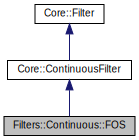
\includegraphics[width=229pt]{class_filters_1_1_continuous_1_1_f_o_s__coll__graph}
\end{center}
\end{figure}


\subsection{Методы}
\hypertarget{class_filters_1_1_continuous_1_1_f_o_s_a6db8005b66c345d94cdd4498edad9022}{}\label{class_filters_1_1_continuous_1_1_f_o_s_a6db8005b66c345d94cdd4498edad9022} 
\index{Filters\+::\+Continuous\+::\+F\+OS@{Filters\+::\+Continuous\+::\+F\+OS}!algorithm@{algorithm}}
\index{algorithm@{algorithm}!Filters\+::\+Continuous\+::\+F\+OS@{Filters\+::\+Continuous\+::\+F\+OS}}
\subsubsection{\texorpdfstring{algorithm()}{algorithm()}}
{\footnotesize\ttfamily void Filters\+::\+Continuous\+::\+F\+O\+S\+::algorithm (\begin{DoxyParamCaption}{ }\end{DoxyParamCaption})\hspace{0.3cm}{\ttfamily [override]}, {\ttfamily [protected]}, {\ttfamily [virtual]}}



Выполняет алгоритм. 

Вектор $Z_t$ оценки вычисляется следующим образом\+: \[dZ_t = a(t,Z_t)dt + K(t,Z_t, \Gamma_t)\cdot [ dY_t - c(t,Z_t)dt],\] \[\Gamma_t = D_t^x - D_t^z,\]

\begin{DoxySeeAlso}{См. также}
\hyperlink{class_core_1_1_continuous_filter}{Core\+::\+Continuous\+Filter} 

\hyperlink{class_core_1_1_continuous_task}{Core\+::\+Continuous\+Task} 
\end{DoxySeeAlso}


Замещает \hyperlink{class_core_1_1_filter_a438681ee3e54aba2148042d9f8011ab8}{Core\+::\+Filter}.



См. определение в файле c\+\_\+fos.\+cc строка 17



Объявления и описания членов классов находятся в файлах\+:\begin{DoxyCompactItemize}
\item 
src/filters/continuous/c\+\_\+fos.\+h\item 
src/filters/continuous/c\+\_\+fos.\+cc\end{DoxyCompactItemize}

\hypertarget{class_filters_1_1_continuous_discrete_1_1_f_o_s}{}\section{Класс Filters\+:\+:Continuous\+Discrete\+:\+:F\+OS}
\label{class_filters_1_1_continuous_discrete_1_1_f_o_s}\index{Filters\+::\+Continuous\+Discrete\+::\+F\+OS@{Filters\+::\+Continuous\+Discrete\+::\+F\+OS}}


Класс, реализующий непрерывно-\/дискретный фильтр оптимальной структуры с непрерывным прогнозом.  




{\ttfamily \#include \char`\"{}cd\+\_\+fos.\+h\char`\"{}}

\subsection*{Открытые члены}
\begin{DoxyCompactItemize}
\item 
\hyperlink{class_filters_1_1_continuous_discrete_1_1_f_o_s_a969ba843b1c5df806d4eb1054d16f4f9}{F\+OS} (\hyperlink{namespace_core_a4811af8148ba137d644b9a61a042cf03}{Core\+::\+Ptr\+Filter\+Parameters} \hyperlink{class_core_1_1_filter_a44aa749b49ba46256975ce545531ecf7}{params}, \hyperlink{namespace_core_abfda8f69fcacfcea2696549b548ed737}{Core\+::\+Ptr\+Task} task)\hypertarget{class_filters_1_1_continuous_discrete_1_1_f_o_s_a969ba843b1c5df806d4eb1054d16f4f9}{}\label{class_filters_1_1_continuous_discrete_1_1_f_o_s_a969ba843b1c5df806d4eb1054d16f4f9}

\begin{DoxyCompactList}\small\item\em Конструктор. \end{DoxyCompactList}\end{DoxyCompactItemize}
\subsection*{Защищенные члены}
\begin{DoxyCompactItemize}
\item 
void \hyperlink{class_filters_1_1_continuous_discrete_1_1_f_o_s_a1e3d6f40678f13a33971bc7bceb45496}{algorithm} () override
\begin{DoxyCompactList}\small\item\em Выполняет алгоритм. \end{DoxyCompactList}\end{DoxyCompactItemize}
\subsection*{Дополнительные унаследованные члены}


\subsection{Подробное описание}
Класс, реализующий непрерывно-\/дискретный фильтр оптимальной структуры с непрерывным прогнозом. 

См. определение в файле cd\+\_\+fos.\+h строка 16



Граф наследования\+:Filters\+:\+:Continuous\+Discrete\+:\+:F\+OS\+:
\nopagebreak
\begin{figure}[H]
\begin{center}
\leavevmode
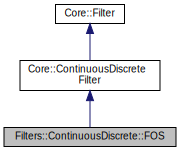
\includegraphics[width=242pt]{class_filters_1_1_continuous_discrete_1_1_f_o_s__inherit__graph}
\end{center}
\end{figure}


Граф связей класса Filters\+:\+:Continuous\+Discrete\+:\+:F\+OS\+:
\nopagebreak
\begin{figure}[H]
\begin{center}
\leavevmode
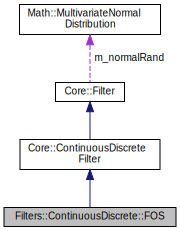
\includegraphics[width=242pt]{class_filters_1_1_continuous_discrete_1_1_f_o_s__coll__graph}
\end{center}
\end{figure}


\subsection{Методы}
\index{Filters\+::\+Continuous\+Discrete\+::\+F\+OS@{Filters\+::\+Continuous\+Discrete\+::\+F\+OS}!algorithm@{algorithm}}
\index{algorithm@{algorithm}!Filters\+::\+Continuous\+Discrete\+::\+F\+OS@{Filters\+::\+Continuous\+Discrete\+::\+F\+OS}}
\subsubsection[{\texorpdfstring{algorithm() override}{algorithm() override}}]{\setlength{\rightskip}{0pt plus 5cm}void Filters\+::\+Continuous\+Discrete\+::\+F\+O\+S\+::algorithm (
\begin{DoxyParamCaption}
{}
\end{DoxyParamCaption}
)\hspace{0.3cm}{\ttfamily [override]}, {\ttfamily [protected]}, {\ttfamily [virtual]}}\hypertarget{class_filters_1_1_continuous_discrete_1_1_f_o_s_a1e3d6f40678f13a33971bc7bceb45496}{}\label{class_filters_1_1_continuous_discrete_1_1_f_o_s_a1e3d6f40678f13a33971bc7bceb45496}


Выполняет алгоритм. 

Вектор $Z_t$ оценки между измерениями вычисляется из уравнения\+: \[\frac{d}{dt}Z_t = \tau(t,Z_t, \Gamma_t).\]

В моменты измерений\+: \[Z_{t_k^+} = Z_{t_k} + \Gamma_{t_k} \cdot G_k^T(Z_{t_k}, \Gamma_{t_k}) \cdot F_k^{-1}(Z_{t_k}, \Gamma_{t_k}) \cdot [Y_k - h_k(Z_{t_k}, \Gamma_{t_k})].\]

Параметр $\Gamma_t$ вычисляется так\+: \[\Gamma_t = D_t^x - D_t^z\]

\begin{DoxySeeAlso}{См. также}
\hyperlink{class_core_1_1_continuous_discrete_filter}{Core\+::\+Continuous\+Discrete\+Filter} 

\hyperlink{class_core_1_1_continuous_discrete_task}{Core\+::\+Continuous\+Discrete\+Task} 
\end{DoxySeeAlso}


Замещает \hyperlink{class_core_1_1_filter_a438681ee3e54aba2148042d9f8011ab8}{Core\+::\+Filter}.



См. определение в файле cd\+\_\+fos.\+cc строка 23



Объявления и описания членов классов находятся в файлах\+:\begin{DoxyCompactItemize}
\item 
src/filters/continuous\+\_\+discrete/cd\+\_\+fos.\+h\item 
src/filters/continuous\+\_\+discrete/cd\+\_\+fos.\+cc\end{DoxyCompactItemize}

\hypertarget{class_filters_1_1_discrete_1_1_f_o_s}{}\section{Класс Filters\+:\+:Discrete\+:\+:F\+OS}
\label{class_filters_1_1_discrete_1_1_f_o_s}\index{Filters\+::\+Discrete\+::\+F\+OS@{Filters\+::\+Discrete\+::\+F\+OS}}


Класс, реализующий дискретный фильтр оптимальной структуры.  




{\ttfamily \#include \char`\"{}d\+\_\+fos.\+h\char`\"{}}

\subsection*{Открытые члены}
\begin{DoxyCompactItemize}
\item 
\hyperlink{class_filters_1_1_discrete_1_1_f_o_s_a4ccb53bc00846f7ca140b55316241749}{F\+OS} (\hyperlink{namespace_core_a4811af8148ba137d644b9a61a042cf03}{Core\+::\+Ptr\+Filter\+Parameters} \hyperlink{class_core_1_1_filter_a44aa749b49ba46256975ce545531ecf7}{params}, \hyperlink{namespace_core_abfda8f69fcacfcea2696549b548ed737}{Core\+::\+Ptr\+Task} task)\hypertarget{class_filters_1_1_discrete_1_1_f_o_s_a4ccb53bc00846f7ca140b55316241749}{}\label{class_filters_1_1_discrete_1_1_f_o_s_a4ccb53bc00846f7ca140b55316241749}

\begin{DoxyCompactList}\small\item\em Конструктор. \end{DoxyCompactList}\end{DoxyCompactItemize}
\subsection*{Защищенные члены}
\begin{DoxyCompactItemize}
\item 
void \hyperlink{class_filters_1_1_discrete_1_1_f_o_s_a66b52dd04e77257393fe156b71e5582f}{algorithm} () override
\begin{DoxyCompactList}\small\item\em Выполняет алгоритм. \end{DoxyCompactList}\end{DoxyCompactItemize}
\subsection*{Закрытые члены}
\begin{DoxyCompactItemize}
\item 
void \hyperlink{class_filters_1_1_discrete_1_1_f_o_s_a2bf612c50a41e892050593ba705c3b79}{compute\+Params} (size\+\_\+t k, Array$<$ Math\+::\+Vector $>$ \&u, Math\+::\+Matrix \&T)
\begin{DoxyCompactList}\small\item\em Вычисляет параметры и заполняет массив $U_k$. \end{DoxyCompactList}\end{DoxyCompactItemize}
\subsection*{Дополнительные унаследованные члены}


\subsection{Подробное описание}
Класс, реализующий дискретный фильтр оптимальной структуры. 

См. определение в файле d\+\_\+fos.\+h строка 16



Граф наследования\+:Filters\+:\+:Discrete\+:\+:F\+OS\+:
\nopagebreak
\begin{figure}[H]
\begin{center}
\leavevmode
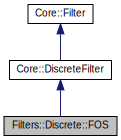
\includegraphics[width=193pt]{class_filters_1_1_discrete_1_1_f_o_s__inherit__graph}
\end{center}
\end{figure}


Граф связей класса Filters\+:\+:Discrete\+:\+:F\+OS\+:
\nopagebreak
\begin{figure}[H]
\begin{center}
\leavevmode
\includegraphics[width=213pt]{class_filters_1_1_discrete_1_1_f_o_s__coll__graph}
\end{center}
\end{figure}


\subsection{Методы}
\index{Filters\+::\+Discrete\+::\+F\+OS@{Filters\+::\+Discrete\+::\+F\+OS}!algorithm@{algorithm}}
\index{algorithm@{algorithm}!Filters\+::\+Discrete\+::\+F\+OS@{Filters\+::\+Discrete\+::\+F\+OS}}
\subsubsection[{\texorpdfstring{algorithm() override}{algorithm() override}}]{\setlength{\rightskip}{0pt plus 5cm}void Filters\+::\+Discrete\+::\+F\+O\+S\+::algorithm (
\begin{DoxyParamCaption}
{}
\end{DoxyParamCaption}
)\hspace{0.3cm}{\ttfamily [override]}, {\ttfamily [protected]}, {\ttfamily [virtual]}}\hypertarget{class_filters_1_1_discrete_1_1_f_o_s_a66b52dd04e77257393fe156b71e5582f}{}\label{class_filters_1_1_discrete_1_1_f_o_s_a66b52dd04e77257393fe156b71e5582f}


Выполняет алгоритм. 

Вектор $Z_t$ оценки вычисляется следующим образом\+: \[\Lambda_k = \tau_{k-1}(U_{k-1}, T_{k-1}),\] \[\Psi_k = \Theta_{k-1}(U_{k-1}, T_{k-1}),\] \[Z_k = \Lambda_k + \Psi_k \cdot G_k^T(\Lambda_k, \Psi_k) \cdot F_k^{-1}(\Lambda_k, \Psi_k) \cdot [Y_k - h_k(\Lambda_k, \Psi_k)].\] \[U_k = \Gamma_k^y \cdot Y_k + \Gamma_k^z \cdot Z_k + \chi_k.\]

Параметры $\Gamma_k^y,\ \Gamma_k^z,\ T_k,\ \chi_k$ вычисляются в \hyperlink{class_filters_1_1_discrete_1_1_f_o_s_a2bf612c50a41e892050593ba705c3b79}{compute\+Params(size\+\_\+t, Array$<$\+Math\+::\+Vector$>$ \&, Math\+::\+Matrix \&)}.

\begin{DoxySeeAlso}{См. также}
\hyperlink{class_core_1_1_discrete_filter}{Core\+::\+Discrete\+Filter} 

\hyperlink{class_core_1_1_discrete_task}{Core\+::\+Discrete\+Task} 
\end{DoxySeeAlso}


Замещает \hyperlink{class_core_1_1_filter_a438681ee3e54aba2148042d9f8011ab8}{Core\+::\+Filter}.



См. определение в файле d\+\_\+fos.\+cc строка 25

\index{Filters\+::\+Discrete\+::\+F\+OS@{Filters\+::\+Discrete\+::\+F\+OS}!compute\+Params@{compute\+Params}}
\index{compute\+Params@{compute\+Params}!Filters\+::\+Discrete\+::\+F\+OS@{Filters\+::\+Discrete\+::\+F\+OS}}
\subsubsection[{\texorpdfstring{compute\+Params(size\+\_\+t k, Array$<$ Math\+::\+Vector $>$ \&u, Math\+::\+Matrix \&\+T)}{computeParams(size_t k, Array< Math::Vector > &u, Math::Matrix &T)}}]{\setlength{\rightskip}{0pt plus 5cm}void Filters\+::\+Discrete\+::\+F\+O\+S\+::compute\+Params (
\begin{DoxyParamCaption}
\item[{size\+\_\+t}]{k, }
\item[{Array$<$ Math\+::\+Vector $>$ \&}]{u, }
\item[{Math\+::\+Matrix \&}]{T}
\end{DoxyParamCaption}
)\hspace{0.3cm}{\ttfamily [private]}}\hypertarget{class_filters_1_1_discrete_1_1_f_o_s_a2bf612c50a41e892050593ba705c3b79}{}\label{class_filters_1_1_discrete_1_1_f_o_s_a2bf612c50a41e892050593ba705c3b79}


Вычисляет параметры и заполняет массив $U_k$. 


\begin{DoxyParams}[1]{Аргументы}
\mbox{\tt in}  & {\em k} & -\/ индекс, соответствующий времени $t = k \cdot \delta t$. \\
\hline
\mbox{\tt out}  & {\em u} & -\/ масcив под выборку $U_k$. \\
\hline
\mbox{\tt out}  & {\em T} & -\/ матрица $T_k$.\\
\hline
\end{DoxyParams}
\[D_k^\delta = cov([Y_k^T\ \ Z_k^T]^T),\] \[[\Gamma_k^y\ \ \Gamma_k^z] = [D_{kk}^{xy}\ \ D_{kk}^{xz}] \cdot (D_k^\delta)^{-1},\] \[\chi_k = m_k^x - \Gamma_k^y \cdot m_k^y - \Gamma_k^z \cdot m_k^z,\] \[T_k = D_k^x - \Gamma_k^y \cdot (D_{kk}^{xy})^T - \Gamma_k^z \cdot (D_{kk}^{xz})^T.\] 

См. определение в файле d\+\_\+fos.\+cc строка 62



Объявления и описания членов классов находятся в файлах\+:\begin{DoxyCompactItemize}
\item 
src/filters/discrete/d\+\_\+fos.\+h\item 
src/filters/discrete/d\+\_\+fos.\+cc\end{DoxyCompactItemize}

\hypertarget{class_core_1_1_function_time}{}\section{Класс Core\+:\+:Function\+Time}
\label{class_core_1_1_function_time}\index{Core\+::\+Function\+Time@{Core\+::\+Function\+Time}}


Базовый класс для классов, представляющих собой функции времени.  




{\ttfamily \#include \char`\"{}function\+\_\+time.\+h\char`\"{}}

\subsection*{Открытые члены}
\begin{DoxyCompactItemize}
\item 
\hypertarget{class_core_1_1_function_time_a7d2987678c02b38563cd21261884d679}{}\label{class_core_1_1_function_time_a7d2987678c02b38563cd21261884d679} 
\hyperlink{class_core_1_1_function_time_a7d2987678c02b38563cd21261884d679}{Function\+Time} (double initial\+Time=0.\+0, double initial\+Step=0.\+001)
\begin{DoxyCompactList}\small\item\em Конструктор. \end{DoxyCompactList}\item 
\hypertarget{class_core_1_1_function_time_a35d2db55f45326b660b9831c6e9ac5c6}{}\label{class_core_1_1_function_time_a35d2db55f45326b660b9831c6e9ac5c6} 
virtual \hyperlink{class_core_1_1_function_time_a35d2db55f45326b660b9831c6e9ac5c6}{$\sim$\+Function\+Time} ()
\begin{DoxyCompactList}\small\item\em Деструктор. \end{DoxyCompactList}\item 
\hypertarget{class_core_1_1_function_time_abdba9d0552e571c23f28335e67cf7f41}{}\label{class_core_1_1_function_time_abdba9d0552e571c23f28335e67cf7f41} 
double \hyperlink{class_core_1_1_function_time_abdba9d0552e571c23f28335e67cf7f41}{time} () const
\begin{DoxyCompactList}\small\item\em Возвращает текущее значение времени. \end{DoxyCompactList}\item 
\hypertarget{class_core_1_1_function_time_a7c3dfc0d8d69c83c162c42435fa13cb9}{}\label{class_core_1_1_function_time_a7c3dfc0d8d69c83c162c42435fa13cb9} 
double \hyperlink{class_core_1_1_function_time_a7c3dfc0d8d69c83c162c42435fa13cb9}{step} () const
\begin{DoxyCompactList}\small\item\em Возвращает шаг на который увеличивается значение времени. \end{DoxyCompactList}\item 
\hypertarget{class_core_1_1_function_time_a0db96b8aff83af1339e08425fe4fd80b}{}\label{class_core_1_1_function_time_a0db96b8aff83af1339e08425fe4fd80b} 
void \hyperlink{class_core_1_1_function_time_a0db96b8aff83af1339e08425fe4fd80b}{set\+Time} (double new\+Time)
\begin{DoxyCompactList}\small\item\em Устанавливает новое значение времени. \end{DoxyCompactList}\item 
\hypertarget{class_core_1_1_function_time_ad1a60dab2d7d8a046893751843c13208}{}\label{class_core_1_1_function_time_ad1a60dab2d7d8a046893751843c13208} 
void \hyperlink{class_core_1_1_function_time_ad1a60dab2d7d8a046893751843c13208}{set\+Step} (double new\+Step)
\begin{DoxyCompactList}\small\item\em Устанавливает шаг на который увеличивается значение времени. \end{DoxyCompactList}\item 
void \hyperlink{class_core_1_1_function_time_a1f1674cdfd0a24f69934467369e30267}{advance\+Time} (double \hyperlink{class_core_1_1_function_time_a7c3dfc0d8d69c83c162c42435fa13cb9}{step})
\begin{DoxyCompactList}\small\item\em Увеличивает значение времни на step. \end{DoxyCompactList}\item 
void \hyperlink{class_core_1_1_function_time_ab2b13d7c42f8a52c2f4ae58efb88ef73}{advance\+Time} ()
\begin{DoxyCompactList}\small\item\em Увеличивает значение времени на величину шага по-\/умолчанию. \end{DoxyCompactList}\end{DoxyCompactItemize}
\subsection*{Защищенные данные}
\begin{DoxyCompactItemize}
\item 
double \hyperlink{class_core_1_1_function_time_a12192d0047976f9cd6376e986e43451c}{m\+\_\+time}
\item 
double \hyperlink{class_core_1_1_function_time_a31d15f7adb8bdecfd22bd35c8fd6eefe}{m\+\_\+step}
\end{DoxyCompactItemize}


\subsection{Подробное описание}
Базовый класс для классов, представляющих собой функции времени. 

Зачем нужен? Позволяет работать со временем там, где нет возможности передать время явно в качестве параметра функции.

Обычный класс, имеющий метод с явной передачей $t$ в параметры\+: 
\begin{DoxyCode}
SomeType func;
\textcolor{keywordtype}{double} t = 10.3;
\textcolor{keywordtype}{double} x = func.foo(..., t);
\end{DoxyCode}
 Класс, унаследованный от \hyperlink{class_core_1_1_function_time}{Function\+Time}\+: 
\begin{DoxyCode}
FunctionTimeChild func;
\textcolor{keywordtype}{double} t = 10.3;
func.setTime(t);
\textcolor{keywordtype}{double} x = func.foo(...);
\end{DoxyCode}
 

См. определение в файле function\+\_\+time.\+h строка 30



Граф наследования\+:Core\+:\+:Function\+Time\+:\nopagebreak
\begin{figure}[H]
\begin{center}
\leavevmode
\includegraphics[width=350pt]{class_core_1_1_function_time__inherit__graph}
\end{center}
\end{figure}


\subsection{Методы}
\hypertarget{class_core_1_1_function_time_a1f1674cdfd0a24f69934467369e30267}{}\label{class_core_1_1_function_time_a1f1674cdfd0a24f69934467369e30267} 
\index{Core\+::\+Function\+Time@{Core\+::\+Function\+Time}!advance\+Time@{advance\+Time}}
\index{advance\+Time@{advance\+Time}!Core\+::\+Function\+Time@{Core\+::\+Function\+Time}}
\subsubsection{\texorpdfstring{advance\+Time()}{advanceTime()}\hspace{0.1cm}{\footnotesize\ttfamily [1/2]}}
{\footnotesize\ttfamily void Core\+::\+Function\+Time\+::advance\+Time (\begin{DoxyParamCaption}\item[{double}]{step }\end{DoxyParamCaption})}



Увеличивает значение времни на step. 

При этом step не сохраняется\+: шаг по-\/умолчанию не изменяется. 

См. определение в файле function\+\_\+time.\+cc строка 38

\hypertarget{class_core_1_1_function_time_ab2b13d7c42f8a52c2f4ae58efb88ef73}{}\label{class_core_1_1_function_time_ab2b13d7c42f8a52c2f4ae58efb88ef73} 
\index{Core\+::\+Function\+Time@{Core\+::\+Function\+Time}!advance\+Time@{advance\+Time}}
\index{advance\+Time@{advance\+Time}!Core\+::\+Function\+Time@{Core\+::\+Function\+Time}}
\subsubsection{\texorpdfstring{advance\+Time()}{advanceTime()}\hspace{0.1cm}{\footnotesize\ttfamily [2/2]}}
{\footnotesize\ttfamily void Core\+::\+Function\+Time\+::advance\+Time (\begin{DoxyParamCaption}{ }\end{DoxyParamCaption})}



Увеличивает значение времени на величину шага по-\/умолчанию. 

Этот шаг задается в конструкторе и может быть изменен вызовом \hyperlink{class_core_1_1_function_time_ad1a60dab2d7d8a046893751843c13208}{set\+Step(double new\+Step)}. 

См. определение в файле function\+\_\+time.\+cc строка 43



\subsection{Данные класса}
\hypertarget{class_core_1_1_function_time_a31d15f7adb8bdecfd22bd35c8fd6eefe}{}\label{class_core_1_1_function_time_a31d15f7adb8bdecfd22bd35c8fd6eefe} 
\index{Core\+::\+Function\+Time@{Core\+::\+Function\+Time}!m\+\_\+step@{m\+\_\+step}}
\index{m\+\_\+step@{m\+\_\+step}!Core\+::\+Function\+Time@{Core\+::\+Function\+Time}}
\subsubsection{\texorpdfstring{m\+\_\+step}{m\_step}}
{\footnotesize\ttfamily double Core\+::\+Function\+Time\+::m\+\_\+step\hspace{0.3cm}{\ttfamily [protected]}}

Шаг. 

См. определение в файле function\+\_\+time.\+h строка 69

\hypertarget{class_core_1_1_function_time_a12192d0047976f9cd6376e986e43451c}{}\label{class_core_1_1_function_time_a12192d0047976f9cd6376e986e43451c} 
\index{Core\+::\+Function\+Time@{Core\+::\+Function\+Time}!m\+\_\+time@{m\+\_\+time}}
\index{m\+\_\+time@{m\+\_\+time}!Core\+::\+Function\+Time@{Core\+::\+Function\+Time}}
\subsubsection{\texorpdfstring{m\+\_\+time}{m\_time}}
{\footnotesize\ttfamily double Core\+::\+Function\+Time\+::m\+\_\+time\hspace{0.3cm}{\ttfamily [protected]}}

Время. 

См. определение в файле function\+\_\+time.\+h строка 68



Объявления и описания членов классов находятся в файлах\+:\begin{DoxyCompactItemize}
\item 
src/core/function\+\_\+time.\+h\item 
src/core/function\+\_\+time.\+cc\end{DoxyCompactItemize}

\hypertarget{struct_g_axis_range}{}\section{Структура G\+Axis\+Range}
\label{struct_g_axis_range}\index{G\+Axis\+Range@{G\+Axis\+Range}}


Структура для хранения границ осей координат.  




{\ttfamily \#include \char`\"{}graph\+\_\+sheet.\+h\char`\"{}}

\subsection*{Открытые атрибуты}
\begin{DoxyCompactItemize}
\item 
double \hyperlink{struct_g_axis_range_a01a9d0fa30092286df72949de7da0d1f}{x\+Min}
\item 
double \hyperlink{struct_g_axis_range_a9ba1a7215788c55bcab90ba3ba87f2de}{x\+Max}
\item 
double \hyperlink{struct_g_axis_range_abc64e1b37194dc086641670a92c62837}{y\+Min}
\item 
double \hyperlink{struct_g_axis_range_a4b2aad8d5fd79b13d555b278ca3b2fb2}{y\+Max}
\end{DoxyCompactItemize}


\subsection{Подробное описание}
Структура для хранения границ осей координат. 

См. определение в файле graph\+\_\+sheet.\+h строка 38



\subsection{Данные класса}
\hypertarget{struct_g_axis_range_a9ba1a7215788c55bcab90ba3ba87f2de}{}\label{struct_g_axis_range_a9ba1a7215788c55bcab90ba3ba87f2de} 
\index{G\+Axis\+Range@{G\+Axis\+Range}!x\+Max@{x\+Max}}
\index{x\+Max@{x\+Max}!G\+Axis\+Range@{G\+Axis\+Range}}
\subsubsection{\texorpdfstring{x\+Max}{xMax}}
{\footnotesize\ttfamily double G\+Axis\+Range\+::x\+Max}

Правая граница оси OX. 

См. определение в файле graph\+\_\+sheet.\+h строка 40

\hypertarget{struct_g_axis_range_a01a9d0fa30092286df72949de7da0d1f}{}\label{struct_g_axis_range_a01a9d0fa30092286df72949de7da0d1f} 
\index{G\+Axis\+Range@{G\+Axis\+Range}!x\+Min@{x\+Min}}
\index{x\+Min@{x\+Min}!G\+Axis\+Range@{G\+Axis\+Range}}
\subsubsection{\texorpdfstring{x\+Min}{xMin}}
{\footnotesize\ttfamily double G\+Axis\+Range\+::x\+Min}

Левая граница оси OX. 

См. определение в файле graph\+\_\+sheet.\+h строка 39

\hypertarget{struct_g_axis_range_a4b2aad8d5fd79b13d555b278ca3b2fb2}{}\label{struct_g_axis_range_a4b2aad8d5fd79b13d555b278ca3b2fb2} 
\index{G\+Axis\+Range@{G\+Axis\+Range}!y\+Max@{y\+Max}}
\index{y\+Max@{y\+Max}!G\+Axis\+Range@{G\+Axis\+Range}}
\subsubsection{\texorpdfstring{y\+Max}{yMax}}
{\footnotesize\ttfamily double G\+Axis\+Range\+::y\+Max}

Верхняя граница оси OY. 

См. определение в файле graph\+\_\+sheet.\+h строка 42

\hypertarget{struct_g_axis_range_abc64e1b37194dc086641670a92c62837}{}\label{struct_g_axis_range_abc64e1b37194dc086641670a92c62837} 
\index{G\+Axis\+Range@{G\+Axis\+Range}!y\+Min@{y\+Min}}
\index{y\+Min@{y\+Min}!G\+Axis\+Range@{G\+Axis\+Range}}
\subsubsection{\texorpdfstring{y\+Min}{yMin}}
{\footnotesize\ttfamily double G\+Axis\+Range\+::y\+Min}

Нижняя граница оси OY. 

См. определение в файле graph\+\_\+sheet.\+h строка 41



Объявления и описания членов структуры находятся в файле\+:\begin{DoxyCompactItemize}
\item 
src/gui/graph\+\_\+sheet.\+h\end{DoxyCompactItemize}

\hypertarget{struct_g_curve}{}\section{Структура G\+Curve}
\label{struct_g_curve}\index{G\+Curve@{G\+Curve}}


Структура для хранения кривой.  




{\ttfamily \#include \char`\"{}graph\+\_\+sheet.\+h\char`\"{}}

\subsection*{Открытые члены}
\begin{DoxyCompactItemize}
\item 
\hypertarget{struct_g_curve_aac51f0bf1cb305e7872d94ee88eef9ba}{}\label{struct_g_curve_aac51f0bf1cb305e7872d94ee88eef9ba} 
\hyperlink{struct_g_curve_aac51f0bf1cb305e7872d94ee88eef9ba}{G\+Curve} ()
\begin{DoxyCompactList}\small\item\em Конструктор. \end{DoxyCompactList}\item 
Q\+String \hyperlink{struct_g_curve_ad9ab2e3ed72e50aaf536db8b961987cc}{full\+Name} () const
\begin{DoxyCompactList}\small\item\em Имя, которое будет отображаться в легенде. \end{DoxyCompactList}\end{DoxyCompactItemize}
\subsection*{Открытые атрибуты}
\begin{DoxyCompactItemize}
\item 
Q\+Vector$<$ double $>$ \hyperlink{struct_g_curve_af4a77d5615109cd4068e11dcc2b52615}{x}
\item 
Q\+Vector$<$ double $>$ \hyperlink{struct_g_curve_a40d381ce3d5ea2ccf654b9e35a8f594b}{y}
\item 
Q\+String \hyperlink{struct_g_curve_a39cc624ec8dffac8afb249e9c6861b88}{name}
\item 
int \hyperlink{struct_g_curve_a67acaf70967bdbaa8c02c614502baacc}{number}
\item 
Q\+Pen \hyperlink{struct_g_curve_ac3f500b2153788be5232dc7a623354ce}{pen}
\item 
bool \hyperlink{struct_g_curve_ac00a68184b569dda559808f50729f96a}{visible}
\end{DoxyCompactItemize}


\subsection{Подробное описание}
Структура для хранения кривой. 

Содержит сами данные (точки), а также информацию о том, как кривая должна рисоваться и подписываться. 

См. определение в файле graph\+\_\+sheet.\+h строка 13



\subsection{Методы}
\hypertarget{struct_g_curve_ad9ab2e3ed72e50aaf536db8b961987cc}{}\label{struct_g_curve_ad9ab2e3ed72e50aaf536db8b961987cc} 
\index{G\+Curve@{G\+Curve}!full\+Name@{full\+Name}}
\index{full\+Name@{full\+Name}!G\+Curve@{G\+Curve}}
\subsubsection{\texorpdfstring{full\+Name()}{fullName()}}
{\footnotesize\ttfamily Q\+String G\+Curve\+::full\+Name (\begin{DoxyParamCaption}{ }\end{DoxyParamCaption}) const}



Имя, которое будет отображаться в легенде. 

Если number == 1, то возвращает строку name без изменений.

Иначе добавляет порядковый номер в конец (не меняя поле name). 

См. определение в файле graph\+\_\+sheet.\+cc строка 12



\subsection{Данные класса}
\hypertarget{struct_g_curve_a39cc624ec8dffac8afb249e9c6861b88}{}\label{struct_g_curve_a39cc624ec8dffac8afb249e9c6861b88} 
\index{G\+Curve@{G\+Curve}!name@{name}}
\index{name@{name}!G\+Curve@{G\+Curve}}
\subsubsection{\texorpdfstring{name}{name}}
{\footnotesize\ttfamily Q\+String G\+Curve\+::name}

Название кривой. 

См. определение в файле graph\+\_\+sheet.\+h строка 28

\hypertarget{struct_g_curve_a67acaf70967bdbaa8c02c614502baacc}{}\label{struct_g_curve_a67acaf70967bdbaa8c02c614502baacc} 
\index{G\+Curve@{G\+Curve}!number@{number}}
\index{number@{number}!G\+Curve@{G\+Curve}}
\subsubsection{\texorpdfstring{number}{number}}
{\footnotesize\ttfamily int G\+Curve\+::number}

Количество кривых с таким же названием. 

См. определение в файле graph\+\_\+sheet.\+h строка 29

\hypertarget{struct_g_curve_ac3f500b2153788be5232dc7a623354ce}{}\label{struct_g_curve_ac3f500b2153788be5232dc7a623354ce} 
\index{G\+Curve@{G\+Curve}!pen@{pen}}
\index{pen@{pen}!G\+Curve@{G\+Curve}}
\subsubsection{\texorpdfstring{pen}{pen}}
{\footnotesize\ttfamily Q\+Pen G\+Curve\+::pen}

Экземпляр Q\+Pen, которым будет рисоваться кривая. 

См. определение в файле graph\+\_\+sheet.\+h строка 30

\hypertarget{struct_g_curve_ac00a68184b569dda559808f50729f96a}{}\label{struct_g_curve_ac00a68184b569dda559808f50729f96a} 
\index{G\+Curve@{G\+Curve}!visible@{visible}}
\index{visible@{visible}!G\+Curve@{G\+Curve}}
\subsubsection{\texorpdfstring{visible}{visible}}
{\footnotesize\ttfamily bool G\+Curve\+::visible}

Видимость кривой (отображается или скрыта?) 

См. определение в файле graph\+\_\+sheet.\+h строка 31

\hypertarget{struct_g_curve_af4a77d5615109cd4068e11dcc2b52615}{}\label{struct_g_curve_af4a77d5615109cd4068e11dcc2b52615} 
\index{G\+Curve@{G\+Curve}!x@{x}}
\index{x@{x}!G\+Curve@{G\+Curve}}
\subsubsection{\texorpdfstring{x}{x}}
{\footnotesize\ttfamily Q\+Vector$<$double$>$ G\+Curve\+::x}

Массив координат $x$ точек $p = (x,y)$. 

См. определение в файле graph\+\_\+sheet.\+h строка 26

\hypertarget{struct_g_curve_a40d381ce3d5ea2ccf654b9e35a8f594b}{}\label{struct_g_curve_a40d381ce3d5ea2ccf654b9e35a8f594b} 
\index{G\+Curve@{G\+Curve}!y@{y}}
\index{y@{y}!G\+Curve@{G\+Curve}}
\subsubsection{\texorpdfstring{y}{y}}
{\footnotesize\ttfamily Q\+Vector$<$double$>$ G\+Curve\+::y}

Массив координат $y$ точек $p = (x,y)$. 

См. определение в файле graph\+\_\+sheet.\+h строка 27



Объявления и описания членов структур находятся в файлах\+:\begin{DoxyCompactItemize}
\item 
src/gui/graph\+\_\+sheet.\+h\item 
src/gui/graph\+\_\+sheet.\+cc\end{DoxyCompactItemize}

\hypertarget{class_graph_sheet}{}\section{Класс Graph\+Sheet}
\label{class_graph_sheet}\index{Graph\+Sheet@{Graph\+Sheet}}


Класс, реализующий \char`\"{}страницу\char`\"{} окна графиков.  




{\ttfamily \#include \char`\"{}graph\+\_\+sheet.\+h\char`\"{}}

\subsection*{Открытые члены}
\begin{DoxyCompactItemize}
\item 
\hypertarget{class_graph_sheet_aad9e497cfb489af37227147397ab021b}{}\label{class_graph_sheet_aad9e497cfb489af37227147397ab021b} 
\hyperlink{class_graph_sheet_aad9e497cfb489af37227147397ab021b}{Graph\+Sheet} ()
\begin{DoxyCompactList}\small\item\em Конструктор. \end{DoxyCompactList}\item 
\hypertarget{class_graph_sheet_ae4511be48b18851127b544cbf099d8e4}{}\label{class_graph_sheet_ae4511be48b18851127b544cbf099d8e4} 
\hyperlink{class_graph_sheet_ae4511be48b18851127b544cbf099d8e4}{$\sim$\+Graph\+Sheet} ()
\begin{DoxyCompactList}\small\item\em Деструктор. \end{DoxyCompactList}\item 
\hypertarget{class_graph_sheet_a63677ef6de3a86eb27bef2ae91993a7c}{}\label{class_graph_sheet_a63677ef6de3a86eb27bef2ae91993a7c} 
void \hyperlink{class_graph_sheet_a63677ef6de3a86eb27bef2ae91993a7c}{clear} ()
\begin{DoxyCompactList}\small\item\em Удаляет все пользовательские данные, устанавливает значения по-\/умолчанию. \end{DoxyCompactList}\item 
\hypertarget{class_graph_sheet_a3684092b56d4b44c41a2d50d3ba3346e}{}\label{class_graph_sheet_a3684092b56d4b44c41a2d50d3ba3346e} 
const Q\+String \& \hyperlink{class_graph_sheet_a3684092b56d4b44c41a2d50d3ba3346e}{x\+Label} () const
\begin{DoxyCompactList}\small\item\em Возвращает подпись для оси OX. \end{DoxyCompactList}\item 
\hypertarget{class_graph_sheet_aaa6ab077b521dbf9e1d7f9fd67f239ac}{}\label{class_graph_sheet_aaa6ab077b521dbf9e1d7f9fd67f239ac} 
const Q\+String \& \hyperlink{class_graph_sheet_aaa6ab077b521dbf9e1d7f9fd67f239ac}{y\+Label} () const
\begin{DoxyCompactList}\small\item\em Возвращает подпись для оси OY. \end{DoxyCompactList}\item 
\hypertarget{class_graph_sheet_a9fcfbe64aa23e4886085e1d000b76728}{}\label{class_graph_sheet_a9fcfbe64aa23e4886085e1d000b76728} 
const Q\+String \& \hyperlink{class_graph_sheet_a9fcfbe64aa23e4886085e1d000b76728}{title\+Label} () const
\begin{DoxyCompactList}\small\item\em Возвращает заголовок страницы. \end{DoxyCompactList}\item 
\hypertarget{class_graph_sheet_a6adc16508129da20d14cea23b289d99c}{}\label{class_graph_sheet_a6adc16508129da20d14cea23b289d99c} 
const Q\+String \& \hyperlink{class_graph_sheet_a6adc16508129da20d14cea23b289d99c}{sub\+Title\+Label} () const
\begin{DoxyCompactList}\small\item\em Возвращает подзаголовок страницы. \end{DoxyCompactList}\item 
\hypertarget{class_graph_sheet_ac13787fb3357ea7d4f3ee3aa4351b0d7}{}\label{class_graph_sheet_ac13787fb3357ea7d4f3ee3aa4351b0d7} 
const \hyperlink{struct_g_axis_range}{G\+Axis\+Range} \& \hyperlink{class_graph_sheet_ac13787fb3357ea7d4f3ee3aa4351b0d7}{axis\+Range} () const
\begin{DoxyCompactList}\small\item\em Возвращает текущие значения границ осей координат. \end{DoxyCompactList}\item 
\hypertarget{class_graph_sheet_a9f2c2ea18ef1ae736366de52cae6909a}{}\label{class_graph_sheet_a9f2c2ea18ef1ae736366de52cae6909a} 
bool \hyperlink{class_graph_sheet_a9f2c2ea18ef1ae736366de52cae6909a}{auto\+Calc\+Ranges} () const
\begin{DoxyCompactList}\small\item\em Возвращает информацию о том, вычисляются границы осей координат автоматически или нет. \end{DoxyCompactList}\item 
\hypertarget{class_graph_sheet_a31e3bbc91be8169bf5014601cea0cf54}{}\label{class_graph_sheet_a31e3bbc91be8169bf5014601cea0cf54} 
const Q\+Vector$<$ \hyperlink{struct_g_curve}{G\+Curve} $>$ \& \hyperlink{class_graph_sheet_a31e3bbc91be8169bf5014601cea0cf54}{curves} () const
\begin{DoxyCompactList}\small\item\em Возвращает ссылку на массив кривых. \end{DoxyCompactList}\item 
\hypertarget{class_graph_sheet_a621fe5716930326ee98375236b20522f}{}\label{class_graph_sheet_a621fe5716930326ee98375236b20522f} 
void \hyperlink{class_graph_sheet_a621fe5716930326ee98375236b20522f}{set\+X\+Label} (const Q\+String \&label)
\begin{DoxyCompactList}\small\item\em Устанавливает подпись для оси OX. \end{DoxyCompactList}\item 
\hypertarget{class_graph_sheet_a121f2bf52435af3924a5fe813456638e}{}\label{class_graph_sheet_a121f2bf52435af3924a5fe813456638e} 
void \hyperlink{class_graph_sheet_a121f2bf52435af3924a5fe813456638e}{set\+Y\+Label} (const Q\+String \&label)
\begin{DoxyCompactList}\small\item\em Устанавливает подпись для оси OY. \end{DoxyCompactList}\item 
\hypertarget{class_graph_sheet_abd3f11230cf41fa15df2c86ad630cbd0}{}\label{class_graph_sheet_abd3f11230cf41fa15df2c86ad630cbd0} 
void \hyperlink{class_graph_sheet_abd3f11230cf41fa15df2c86ad630cbd0}{set\+Title\+Label} (const Q\+String \&label)
\begin{DoxyCompactList}\small\item\em Устанавливает заголовок страницы. \end{DoxyCompactList}\item 
\hypertarget{class_graph_sheet_a0ecbf848f6d821e9fd5b6806c88a178c}{}\label{class_graph_sheet_a0ecbf848f6d821e9fd5b6806c88a178c} 
void \hyperlink{class_graph_sheet_a0ecbf848f6d821e9fd5b6806c88a178c}{set\+Sub\+Title\+Label} (const Q\+String \&label)
\begin{DoxyCompactList}\small\item\em Устанавливает подзаголовок страницы. \end{DoxyCompactList}\item 
void \hyperlink{class_graph_sheet_a5ac1eac707300dc2e8d856e49bd797f3}{set\+Auto\+Calc\+Ranges} (bool auto\+Calc)
\begin{DoxyCompactList}\small\item\em Устанавливает метод работы с границами осей координат. \end{DoxyCompactList}\item 
\hypertarget{class_graph_sheet_ae37cc5b56c35ae34ced47c6f21eebf45}{}\label{class_graph_sheet_ae37cc5b56c35ae34ced47c6f21eebf45} 
void \hyperlink{class_graph_sheet_ae37cc5b56c35ae34ced47c6f21eebf45}{set\+Axis\+Range} (const \hyperlink{struct_g_axis_range}{G\+Axis\+Range} \&\hyperlink{class_graph_sheet_ac13787fb3357ea7d4f3ee3aa4351b0d7}{axis\+Range})
\begin{DoxyCompactList}\small\item\em Сохраняет пользовательские границы осей координат. \end{DoxyCompactList}\item 
void \hyperlink{class_graph_sheet_af8f3efaf2a6ba860b089bef15e07f403}{set\+Curve\+Visible} (int index, bool visible)
\begin{DoxyCompactList}\small\item\em Устанавливает видимость кривой. \end{DoxyCompactList}\item 
void \hyperlink{class_graph_sheet_abce999772aca9f5da197f13fd8912362}{add\+Curve} (const Q\+Vector$<$ double $>$ \&x, const Q\+Vector$<$ double $>$ \&y, const Q\+String \&name, const Q\+Pen \&pen, bool visible=true)
\begin{DoxyCompactList}\small\item\em Добавляет новую кривую. \end{DoxyCompactList}\end{DoxyCompactItemize}
\subsection*{Закрытые члены}
\begin{DoxyCompactItemize}
\item 
void \hyperlink{class_graph_sheet_adc73499b0d6b96dde2e3d1f829ec6273}{calc\+Ranges} ()
\begin{DoxyCompactList}\small\item\em Устанавливает границы осей координат. \end{DoxyCompactList}\end{DoxyCompactItemize}
\subsection*{Закрытые данные}
\begin{DoxyCompactItemize}
\item 
\hypertarget{class_graph_sheet_a970d65cbe6e836277bbf845962c84289}{}\label{class_graph_sheet_a970d65cbe6e836277bbf845962c84289} 
Q\+Vector$<$ \hyperlink{struct_g_curve}{G\+Curve} $>$ {\bfseries m\+\_\+curves}
\item 
\hypertarget{class_graph_sheet_a44b18b8ca129276833d543f0faf70008}{}\label{class_graph_sheet_a44b18b8ca129276833d543f0faf70008} 
Q\+String {\bfseries m\+\_\+x\+Label}
\item 
\hypertarget{class_graph_sheet_a65c42e7ee50cff1b41f200747c99b230}{}\label{class_graph_sheet_a65c42e7ee50cff1b41f200747c99b230} 
Q\+String {\bfseries m\+\_\+y\+Label}
\item 
\hypertarget{class_graph_sheet_a85647d1e1446c66ca9e215db1e3ab9a3}{}\label{class_graph_sheet_a85647d1e1446c66ca9e215db1e3ab9a3} 
Q\+String {\bfseries m\+\_\+title\+Label}
\item 
\hypertarget{class_graph_sheet_aad55c740b2576ea491f66c83695395bb}{}\label{class_graph_sheet_aad55c740b2576ea491f66c83695395bb} 
Q\+String {\bfseries m\+\_\+sub\+Title\+Label}
\item 
\hypertarget{class_graph_sheet_a326acf4c64a807219abbd635482c370c}{}\label{class_graph_sheet_a326acf4c64a807219abbd635482c370c} 
bool {\bfseries m\+\_\+auto\+Calc\+Ranges}
\item 
\hypertarget{class_graph_sheet_a80184036212ce75a2c4799da5032f237}{}\label{class_graph_sheet_a80184036212ce75a2c4799da5032f237} 
\hyperlink{struct_g_axis_range}{G\+Axis\+Range} {\bfseries m\+\_\+axis\+Range}
\item 
\hypertarget{class_graph_sheet_a614acb7954caf3e7c28350d37bc8a6ca}{}\label{class_graph_sheet_a614acb7954caf3e7c28350d37bc8a6ca} 
\hyperlink{struct_g_axis_range}{G\+Axis\+Range} {\bfseries m\+\_\+user\+Axis\+Range}
\end{DoxyCompactItemize}


\subsection{Подробное описание}
Класс, реализующий \char`\"{}страницу\char`\"{} окна графиков. 

Хранит в себе данные всех кривых, отображаемых на странице и предоставляет пользователю возможности настройки отображения.

Ничего не рисует, только работает с данными. Отрисовкой занимается \hyperlink{class_graph_window}{Graph\+Window}. 

См. определение в файле graph\+\_\+sheet.\+h строка 55



Граф связей класса Graph\+Sheet\+:\nopagebreak
\begin{figure}[H]
\begin{center}
\leavevmode
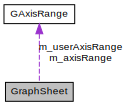
\includegraphics[width=199pt]{class_graph_sheet__coll__graph}
\end{center}
\end{figure}


\subsection{Методы}
\hypertarget{class_graph_sheet_abce999772aca9f5da197f13fd8912362}{}\label{class_graph_sheet_abce999772aca9f5da197f13fd8912362} 
\index{Graph\+Sheet@{Graph\+Sheet}!add\+Curve@{add\+Curve}}
\index{add\+Curve@{add\+Curve}!Graph\+Sheet@{Graph\+Sheet}}
\subsubsection{\texorpdfstring{add\+Curve()}{addCurve()}}
{\footnotesize\ttfamily void Graph\+Sheet\+::add\+Curve (\begin{DoxyParamCaption}\item[{const Q\+Vector$<$ double $>$ \&}]{x,  }\item[{const Q\+Vector$<$ double $>$ \&}]{y,  }\item[{const Q\+String \&}]{name,  }\item[{const Q\+Pen \&}]{pen,  }\item[{bool}]{visible = {\ttfamily true} }\end{DoxyParamCaption})}



Добавляет новую кривую. 


\begin{DoxyParams}{Аргументы}
{\em x} & -\/ массив координат $x$ точек $p = (x,y)$. \\
\hline
{\em y} & -\/ массив координат $y$ точек $p = (x,y)$. \\
\hline
{\em name} & -\/ название кривой. \\
\hline
{\em pen} & -\/ экземпляр Q\+Pen, которым будет рисоваться кривая. \\
\hline
{\em visible} & -\/ видимость кривой (отображается или скрыта?) \\
\hline
\end{DoxyParams}


См. определение в файле graph\+\_\+sheet.\+cc строка 124

\hypertarget{class_graph_sheet_adc73499b0d6b96dde2e3d1f829ec6273}{}\label{class_graph_sheet_adc73499b0d6b96dde2e3d1f829ec6273} 
\index{Graph\+Sheet@{Graph\+Sheet}!calc\+Ranges@{calc\+Ranges}}
\index{calc\+Ranges@{calc\+Ranges}!Graph\+Sheet@{Graph\+Sheet}}
\subsubsection{\texorpdfstring{calc\+Ranges()}{calcRanges()}}
{\footnotesize\ttfamily void Graph\+Sheet\+::calc\+Ranges (\begin{DoxyParamCaption}{ }\end{DoxyParamCaption})\hspace{0.3cm}{\ttfamily [private]}}



Устанавливает границы осей координат. 

Если m\+\_\+auto\+Calc\+Ranges == true, то вычисляет их, пробегая по всем точкам всех кривых.

Иначе берет их из m\+\_\+user\+Axis\+Range.

Результат сохраняется в m\+\_\+axis\+Range, который возвращается при вызове \hyperlink{class_graph_sheet_ac13787fb3357ea7d4f3ee3aa4351b0d7}{axis\+Range()}. 

См. определение в файле graph\+\_\+sheet.\+cc строка 148

\hypertarget{class_graph_sheet_a5ac1eac707300dc2e8d856e49bd797f3}{}\label{class_graph_sheet_a5ac1eac707300dc2e8d856e49bd797f3} 
\index{Graph\+Sheet@{Graph\+Sheet}!set\+Auto\+Calc\+Ranges@{set\+Auto\+Calc\+Ranges}}
\index{set\+Auto\+Calc\+Ranges@{set\+Auto\+Calc\+Ranges}!Graph\+Sheet@{Graph\+Sheet}}
\subsubsection{\texorpdfstring{set\+Auto\+Calc\+Ranges()}{setAutoCalcRanges()}}
{\footnotesize\ttfamily void Graph\+Sheet\+::set\+Auto\+Calc\+Ranges (\begin{DoxyParamCaption}\item[{bool}]{auto\+Calc }\end{DoxyParamCaption})}



Устанавливает метод работы с границами осей координат. 


\begin{DoxyParams}{Аргументы}
{\em auto\+Calc} & -\/ если true, то границы считаются автоматически, иначе -\/ берутся введенные пользователем вручную данные. \\
\hline
\end{DoxyParams}


См. определение в файле graph\+\_\+sheet.\+cc строка 101

\hypertarget{class_graph_sheet_af8f3efaf2a6ba860b089bef15e07f403}{}\label{class_graph_sheet_af8f3efaf2a6ba860b089bef15e07f403} 
\index{Graph\+Sheet@{Graph\+Sheet}!set\+Curve\+Visible@{set\+Curve\+Visible}}
\index{set\+Curve\+Visible@{set\+Curve\+Visible}!Graph\+Sheet@{Graph\+Sheet}}
\subsubsection{\texorpdfstring{set\+Curve\+Visible()}{setCurveVisible()}}
{\footnotesize\ttfamily void Graph\+Sheet\+::set\+Curve\+Visible (\begin{DoxyParamCaption}\item[{int}]{index,  }\item[{bool}]{visible }\end{DoxyParamCaption})}



Устанавливает видимость кривой. 


\begin{DoxyParams}{Аргументы}
{\em index} & -\/ номер кривой в массиве. \\
\hline
{\em visible} & -\/ если true, то кривая будет отображаться, иначе -\/ скрыта. \\
\hline
\end{DoxyParams}


См. определение в файле graph\+\_\+sheet.\+cc строка 112



Объявления и описания членов классов находятся в файлах\+:\begin{DoxyCompactItemize}
\item 
src/gui/graph\+\_\+sheet.\+h\item 
src/gui/graph\+\_\+sheet.\+cc\end{DoxyCompactItemize}

\hypertarget{class_graph_window}{}\section{Класс Graph\+Window}
\label{class_graph_window}\index{Graph\+Window@{Graph\+Window}}


Класс, реализующий окно для просмотра графиков.  




{\ttfamily \#include \char`\"{}graph\+\_\+window.\+h\char`\"{}}

\subsection*{Открытые слоты}
\begin{DoxyCompactItemize}
\item 
void \hyperlink{class_graph_window_a6f4268aa4bd0780c0016ed6bb74253d3}{on\+Clear} ()\hypertarget{class_graph_window_a6f4268aa4bd0780c0016ed6bb74253d3}{}\label{class_graph_window_a6f4268aa4bd0780c0016ed6bb74253d3}

\begin{DoxyCompactList}\small\item\em Удаляет пользовательские данные, устанавливает значения по-\/умолчанию. \end{DoxyCompactList}\end{DoxyCompactItemize}
\subsection*{Открытые члены}
\begin{DoxyCompactItemize}
\item 
\hyperlink{class_graph_window_a68f193cacc0237a41d8c44923b53c11a}{Graph\+Window} (Q\+Widget $\ast$parent=nullptr)\hypertarget{class_graph_window_a68f193cacc0237a41d8c44923b53c11a}{}\label{class_graph_window_a68f193cacc0237a41d8c44923b53c11a}

\begin{DoxyCompactList}\small\item\em Конструктор. \end{DoxyCompactList}\item 
\hyperlink{class_graph_window_acca1dc8c3eefe6608ae2de3cee2e22ee}{$\sim$\+Graph\+Window} ()\hypertarget{class_graph_window_acca1dc8c3eefe6608ae2de3cee2e22ee}{}\label{class_graph_window_acca1dc8c3eefe6608ae2de3cee2e22ee}

\begin{DoxyCompactList}\small\item\em Деструктор. \end{DoxyCompactList}\item 
int \hyperlink{class_graph_window_a5a433ecbf8a3b30292de59955c5fa4ff}{count\+Sheets} () const \hypertarget{class_graph_window_a5a433ecbf8a3b30292de59955c5fa4ff}{}\label{class_graph_window_a5a433ecbf8a3b30292de59955c5fa4ff}

\begin{DoxyCompactList}\small\item\em Возвращает количество страниц. \end{DoxyCompactList}\item 
\hyperlink{class_graph_sheet}{Graph\+Sheet} \& \hyperlink{class_graph_window_a756c68dacb48b03ac45d457d61a760d8}{sheet} (int index)\hypertarget{class_graph_window_a756c68dacb48b03ac45d457d61a760d8}{}\label{class_graph_window_a756c68dacb48b03ac45d457d61a760d8}

\begin{DoxyCompactList}\small\item\em Возвращает ссылку на страницу с номером index. \end{DoxyCompactList}\item 
\hyperlink{class_graph_sheet}{Graph\+Sheet} \& \hyperlink{class_graph_window_a1e2ba902888b95d5fef9dfe081bac90b}{current\+Sheet} ()\hypertarget{class_graph_window_a1e2ba902888b95d5fef9dfe081bac90b}{}\label{class_graph_window_a1e2ba902888b95d5fef9dfe081bac90b}

\begin{DoxyCompactList}\small\item\em Возвращает ссылку страницу, котороая отображается в данный момент. \end{DoxyCompactList}\item 
void \hyperlink{class_graph_window_af7499e98193373a6322470c5dfe961a8}{set\+Count\+Sheets} (int count)\hypertarget{class_graph_window_af7499e98193373a6322470c5dfe961a8}{}\label{class_graph_window_af7499e98193373a6322470c5dfe961a8}

\begin{DoxyCompactList}\small\item\em Устанавливает количество страниц \end{DoxyCompactList}\item 
void \hyperlink{class_graph_window_acdc8aa7200c0bfddee48a16a0875986a}{update\+Plotter} ()\hypertarget{class_graph_window_acdc8aa7200c0bfddee48a16a0875986a}{}\label{class_graph_window_acdc8aa7200c0bfddee48a16a0875986a}

\begin{DoxyCompactList}\small\item\em Обновляет поле рисовальщика Q\+Custom\+Plot (заставляет перерисовать себя). \end{DoxyCompactList}\end{DoxyCompactItemize}
\subsection*{Закрытые слоты}
\begin{DoxyCompactItemize}
\item 
void \hyperlink{class_graph_window_ab41020bb6d02870bd0f2ccca51cb4837}{on\+Selection\+Changed} ()\hypertarget{class_graph_window_ab41020bb6d02870bd0f2ccca51cb4837}{}\label{class_graph_window_ab41020bb6d02870bd0f2ccca51cb4837}

\begin{DoxyCompactList}\small\item\em Реакция на выделение какого-\/либо объекта мышью на поле рисовальщика. \end{DoxyCompactList}\item 
void \hyperlink{class_graph_window_a678bb0942c6ca67d1ec366ea6c3f9c8e}{on\+Mouse\+Press} ()\hypertarget{class_graph_window_a678bb0942c6ca67d1ec366ea6c3f9c8e}{}\label{class_graph_window_a678bb0942c6ca67d1ec366ea6c3f9c8e}

\begin{DoxyCompactList}\small\item\em Реакция на клик мыши по полю рисовальщика. \end{DoxyCompactList}\item 
void \hyperlink{class_graph_window_a1731d19496de65b3b1a3e125afa8a41a}{on\+Mouse\+Wheel} ()\hypertarget{class_graph_window_a1731d19496de65b3b1a3e125afa8a41a}{}\label{class_graph_window_a1731d19496de65b3b1a3e125afa8a41a}

\begin{DoxyCompactList}\small\item\em Реакция на движение мыши. \end{DoxyCompactList}\item 
void \hyperlink{class_graph_window_a2cc0f9b9b91ccb7c3d203670467a556e}{on\+Menu\+Request} (Q\+Point pos)
\begin{DoxyCompactList}\small\item\em Вызывает контекстное меню. \end{DoxyCompactList}\item 
void \hyperlink{class_graph_window_ac8a8d86f74361c73bf0a75254e7ee069}{on\+Move\+Legend} ()\hypertarget{class_graph_window_ac8a8d86f74361c73bf0a75254e7ee069}{}\label{class_graph_window_ac8a8d86f74361c73bf0a75254e7ee069}

\begin{DoxyCompactList}\small\item\em Перемещает окно легенды внутри поля рисовальщика. \end{DoxyCompactList}\item 
void \hyperlink{class_graph_window_a76559e3f41e482a43f715f519df4487c}{on\+Ranges\+Changed} (Math\+::\+Vector2 x, Math\+::\+Vector2 y)
\begin{DoxyCompactList}\small\item\em Изменяет границы осей координат и перерисовывает картинку. \end{DoxyCompactList}\item 
void \hyperlink{class_graph_window_a51f89adcbef5b90b9fdbb24bf7536fe5}{on\+Save\+Png} ()
\begin{DoxyCompactList}\small\item\em Сохраняет изображение. \end{DoxyCompactList}\item 
void \hyperlink{class_graph_window_aca7c92575aaed2db319bb86a1e1e36e9}{on\+Show\+Set\+Ranges\+Dialog} ()\hypertarget{class_graph_window_aca7c92575aaed2db319bb86a1e1e36e9}{}\label{class_graph_window_aca7c92575aaed2db319bb86a1e1e36e9}

\begin{DoxyCompactList}\small\item\em Показывает окно выбора границ осей координат при нажатии кнопки меню. \end{DoxyCompactList}\item 
void \hyperlink{class_graph_window_ac6e6c5f747d9fc8d4f1988262cf12303}{on\+Set\+Auto\+Ranges} (bool checked)\hypertarget{class_graph_window_ac6e6c5f747d9fc8d4f1988262cf12303}{}\label{class_graph_window_ac6e6c5f747d9fc8d4f1988262cf12303}

\begin{DoxyCompactList}\small\item\em Передает информацию о том, нужно ли автоматически вычислять границы осей координат, в \hyperlink{class_graph_sheet}{Graph\+Sheet}. \end{DoxyCompactList}\item 
void \hyperlink{class_graph_window_aa5e82d18c3767b11b36b1b76cf989054}{on\+Hide\+Curve} (Q\+Action $\ast$action)\hypertarget{class_graph_window_aa5e82d18c3767b11b36b1b76cf989054}{}\label{class_graph_window_aa5e82d18c3767b11b36b1b76cf989054}

\begin{DoxyCompactList}\small\item\em Скрывает выбранную кривую (из главного меню). \end{DoxyCompactList}\item 
void \hyperlink{class_graph_window_a81681956de7261ef2fa6b6ed28e2e903}{on\+Hide\+Curve\+From\+Context\+Menu} ()\hypertarget{class_graph_window_a81681956de7261ef2fa6b6ed28e2e903}{}\label{class_graph_window_a81681956de7261ef2fa6b6ed28e2e903}

\begin{DoxyCompactList}\small\item\em Скрывает выбранную кривую (из контекстного). \end{DoxyCompactList}\item 
void \hyperlink{class_graph_window_a600b5476f121fb83f2d0db599becc73a}{on\+Show\+Curve} (Q\+Action $\ast$action)\hypertarget{class_graph_window_a600b5476f121fb83f2d0db599becc73a}{}\label{class_graph_window_a600b5476f121fb83f2d0db599becc73a}

\begin{DoxyCompactList}\small\item\em Показывает выбранную скрытую кривую. \end{DoxyCompactList}\item 
void \hyperlink{class_graph_window_ad99844f68aa659cdb599681d3cd231b1}{on\+Current\+Sheet\+Changed} (Q\+Action $\ast$action)\hypertarget{class_graph_window_ad99844f68aa659cdb599681d3cd231b1}{}\label{class_graph_window_ad99844f68aa659cdb599681d3cd231b1}

\begin{DoxyCompactList}\small\item\em Перерисовыет содержимое поля рисовальщика при смене страницы (из меню). \end{DoxyCompactList}\end{DoxyCompactItemize}
\subsection*{Закрытые члены}
\begin{DoxyCompactItemize}
\item 
void \hyperlink{class_graph_window_ad4d4842869a043556a275ba06acd816b}{load\+Fonts} ()
\begin{DoxyCompactList}\small\item\em Загружает шрифты и устанавливает их параметры (начертание, размер и т.\+д.). \end{DoxyCompactList}\item 
void \hyperlink{class_graph_window_ad793717ed7de5d225e90c8ebe29474e3}{init\+Layouts} ()\hypertarget{class_graph_window_ad793717ed7de5d225e90c8ebe29474e3}{}\label{class_graph_window_ad793717ed7de5d225e90c8ebe29474e3}

\begin{DoxyCompactList}\small\item\em Устанавливает расположение всех элементов на виджете. \end{DoxyCompactList}\item 
void \hyperlink{class_graph_window_a5c8eb0b2281c1d099b5fbe0dc4d8081e}{init\+Actions} ()\hypertarget{class_graph_window_a5c8eb0b2281c1d099b5fbe0dc4d8081e}{}\label{class_graph_window_a5c8eb0b2281c1d099b5fbe0dc4d8081e}

\begin{DoxyCompactList}\small\item\em Инициализирует элементы Q\+Action меню. \end{DoxyCompactList}\item 
void \hyperlink{class_graph_window_aaac43b54c4d10097e161dea8f3280f11}{init\+Menus} ()\hypertarget{class_graph_window_aaac43b54c4d10097e161dea8f3280f11}{}\label{class_graph_window_aaac43b54c4d10097e161dea8f3280f11}

\begin{DoxyCompactList}\small\item\em Инициализирует главное меню и связывает элементы с соответствующими Q\+Actions. \end{DoxyCompactList}\item 
void \hyperlink{class_graph_window_af9dac0c26f2353aa799075ca0d710490}{init\+Plotter} ()\hypertarget{class_graph_window_af9dac0c26f2353aa799075ca0d710490}{}\label{class_graph_window_af9dac0c26f2353aa799075ca0d710490}

\begin{DoxyCompactList}\small\item\em Инициализирует поле рисовальщика Q\+Custom\+Plot. \end{DoxyCompactList}\item 
void \hyperlink{class_graph_window_a91cd37369dcf09153d6088686dc720b1}{update\+Menu} ()\hypertarget{class_graph_window_a91cd37369dcf09153d6088686dc720b1}{}\label{class_graph_window_a91cd37369dcf09153d6088686dc720b1}

\begin{DoxyCompactList}\small\item\em Обновляет элементы главного меню при необходимости. \end{DoxyCompactList}\end{DoxyCompactItemize}
\subsection*{Закрытые данные}
\begin{DoxyCompactItemize}
\item 
Q\+Vector$<$ \hyperlink{class_graph_sheet}{Graph\+Sheet} $>$ {\bfseries m\+\_\+sheets}\hypertarget{class_graph_window_a03b672b398d6659d8b3c45cb0bb3b678}{}\label{class_graph_window_a03b672b398d6659d8b3c45cb0bb3b678}

\item 
\hyperlink{class_graph_sheet}{Graph\+Sheet} $\ast$ {\bfseries m\+\_\+current\+Sheet}\hypertarget{class_graph_window_afb61e9bb808e6699aa29cd62e92d185a}{}\label{class_graph_window_afb61e9bb808e6699aa29cd62e92d185a}

\item 
Q\+Custom\+Plot $\ast$ {\bfseries m\+\_\+plotter}\hypertarget{class_graph_window_add927bb710c37931242a670757d728ea}{}\label{class_graph_window_add927bb710c37931242a670757d728ea}

\item 
Q\+Font {\bfseries m\+\_\+plotter\+Title\+Font}\hypertarget{class_graph_window_af89ca6d320439fa29acb09381d6b5518}{}\label{class_graph_window_af89ca6d320439fa29acb09381d6b5518}

\item 
Q\+Font {\bfseries m\+\_\+plotter\+Sub\+Title\+Font}\hypertarget{class_graph_window_a050668ab58e0cd8b9284f4ceeba882ff}{}\label{class_graph_window_a050668ab58e0cd8b9284f4ceeba882ff}

\item 
Q\+Font {\bfseries m\+\_\+plotter\+Legend\+Font}\hypertarget{class_graph_window_a4072100eb0280206cb00f254f49e72e0}{}\label{class_graph_window_a4072100eb0280206cb00f254f49e72e0}

\item 
Q\+Font {\bfseries m\+\_\+plotter\+Axes\+Label\+Font}\hypertarget{class_graph_window_a6a2deb2327b56849d617fa00bc38814c}{}\label{class_graph_window_a6a2deb2327b56849d617fa00bc38814c}

\item 
Q\+Font {\bfseries m\+\_\+plotter\+Axes\+Tick\+Label\+Font}\hypertarget{class_graph_window_a7c5bc426aef2b19679ecb9ce7a5f688e}{}\label{class_graph_window_a7c5bc426aef2b19679ecb9ce7a5f688e}

\item 
Q\+Action $\ast$ {\bfseries m\+\_\+action\+Save\+Png}\hypertarget{class_graph_window_a8b18154ef9c7f978df94dbae8855d30a}{}\label{class_graph_window_a8b18154ef9c7f978df94dbae8855d30a}

\item 
Q\+Action $\ast$ {\bfseries m\+\_\+action\+Show\+Set\+Ranges\+Dialog}\hypertarget{class_graph_window_a6c342da9e826998d3744ec87d5a710a4}{}\label{class_graph_window_a6c342da9e826998d3744ec87d5a710a4}

\item 
Q\+Action $\ast$ {\bfseries m\+\_\+action\+Set\+Auto\+Ranges}\hypertarget{class_graph_window_add86d9623399b3aaace9c961c2c56d9f}{}\label{class_graph_window_add86d9623399b3aaace9c961c2c56d9f}

\item 
Q\+Menu $\ast$ {\bfseries m\+\_\+menu\+File}\hypertarget{class_graph_window_a2cfe856a0c10dfffb05e4a568d135feb}{}\label{class_graph_window_a2cfe856a0c10dfffb05e4a568d135feb}

\item 
Q\+Menu $\ast$ {\bfseries m\+\_\+menu\+View}\hypertarget{class_graph_window_a3e2ffe57452e156a0d62fb82da8ed868}{}\label{class_graph_window_a3e2ffe57452e156a0d62fb82da8ed868}

\item 
Q\+Menu $\ast$ {\bfseries m\+\_\+menu\+Sheet}\hypertarget{class_graph_window_ae3c17a4c2fc6e3f935dc3b3f7cc89974}{}\label{class_graph_window_ae3c17a4c2fc6e3f935dc3b3f7cc89974}

\item 
Q\+Menu $\ast$ {\bfseries m\+\_\+menu\+Show}\hypertarget{class_graph_window_a4078c2f892ffb57912412fb0c38af5ba}{}\label{class_graph_window_a4078c2f892ffb57912412fb0c38af5ba}

\item 
Q\+Menu $\ast$ {\bfseries m\+\_\+menu\+Hide}\hypertarget{class_graph_window_a2df057f6b70c12d9190a456a7f62b9c4}{}\label{class_graph_window_a2df057f6b70c12d9190a456a7f62b9c4}

\end{DoxyCompactItemize}


\subsection{Подробное описание}
Класс, реализующий окно для просмотра графиков. 

См. определение в файле graph\+\_\+window.\+h строка 24



Граф наследования\+:Graph\+Window\+:
\nopagebreak
\begin{figure}[H]
\begin{center}
\leavevmode
\includegraphics[width=160pt]{class_graph_window__inherit__graph}
\end{center}
\end{figure}


Граф связей класса Graph\+Window\+:
\nopagebreak
\begin{figure}[H]
\begin{center}
\leavevmode
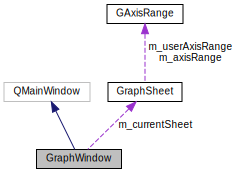
\includegraphics[width=296pt]{class_graph_window__coll__graph}
\end{center}
\end{figure}


\subsection{Методы}
\index{Graph\+Window@{Graph\+Window}!load\+Fonts@{load\+Fonts}}
\index{load\+Fonts@{load\+Fonts}!Graph\+Window@{Graph\+Window}}
\subsubsection[{\texorpdfstring{load\+Fonts()}{loadFonts()}}]{\setlength{\rightskip}{0pt plus 5cm}void Graph\+Window\+::load\+Fonts (
\begin{DoxyParamCaption}
{}
\end{DoxyParamCaption}
)\hspace{0.3cm}{\ttfamily [private]}}\hypertarget{class_graph_window_ad4d4842869a043556a275ba06acd816b}{}\label{class_graph_window_ad4d4842869a043556a275ba06acd816b}


Загружает шрифты и устанавливает их параметры (начертание, размер и т.\+д.). 

\begin{DoxySeeAlso}{См. также}
\hyperlink{class_font_manager}{Font\+Manager}. 
\end{DoxySeeAlso}


См. определение в файле graph\+\_\+window.\+cc строка 19

\index{Graph\+Window@{Graph\+Window}!on\+Menu\+Request@{on\+Menu\+Request}}
\index{on\+Menu\+Request@{on\+Menu\+Request}!Graph\+Window@{Graph\+Window}}
\subsubsection[{\texorpdfstring{on\+Menu\+Request}{onMenuRequest}}]{\setlength{\rightskip}{0pt plus 5cm}void Graph\+Window\+::on\+Menu\+Request (
\begin{DoxyParamCaption}
\item[{Q\+Point}]{pos}
\end{DoxyParamCaption}
)\hspace{0.3cm}{\ttfamily [private]}, {\ttfamily [slot]}}\hypertarget{class_graph_window_a2cc0f9b9b91ccb7c3d203670467a556e}{}\label{class_graph_window_a2cc0f9b9b91ccb7c3d203670467a556e}


Вызывает контекстное меню. 

Слот. Реакция на клик правой кнопкой мыши внутри поля рисовальщика. 

См. определение в файле graph\+\_\+window.\+cc строка 254

\index{Graph\+Window@{Graph\+Window}!on\+Ranges\+Changed@{on\+Ranges\+Changed}}
\index{on\+Ranges\+Changed@{on\+Ranges\+Changed}!Graph\+Window@{Graph\+Window}}
\subsubsection[{\texorpdfstring{on\+Ranges\+Changed}{onRangesChanged}}]{\setlength{\rightskip}{0pt plus 5cm}void Graph\+Window\+::on\+Ranges\+Changed (
\begin{DoxyParamCaption}
\item[{Math\+::\+Vector2}]{x, }
\item[{Math\+::\+Vector2}]{y}
\end{DoxyParamCaption}
)\hspace{0.3cm}{\ttfamily [private]}, {\ttfamily [slot]}}\hypertarget{class_graph_window_a76559e3f41e482a43f715f519df4487c}{}\label{class_graph_window_a76559e3f41e482a43f715f519df4487c}


Изменяет границы осей координат и перерисовывает картинку. 


\begin{DoxyParams}{Аргументы}
{\em x} & -\/ пара (min, max) для оси OX. \\
\hline
{\em y} & -\/ пара (min, max) для оси OY. \\
\hline
\end{DoxyParams}


См. определение в файле graph\+\_\+window.\+cc строка 293

\index{Graph\+Window@{Graph\+Window}!on\+Save\+Png@{on\+Save\+Png}}
\index{on\+Save\+Png@{on\+Save\+Png}!Graph\+Window@{Graph\+Window}}
\subsubsection[{\texorpdfstring{on\+Save\+Png}{onSavePng}}]{\setlength{\rightskip}{0pt plus 5cm}void Graph\+Window\+::on\+Save\+Png (
\begin{DoxyParamCaption}
{}
\end{DoxyParamCaption}
)\hspace{0.3cm}{\ttfamily [private]}, {\ttfamily [slot]}}\hypertarget{class_graph_window_a51f89adcbef5b90b9fdbb24bf7536fe5}{}\label{class_graph_window_a51f89adcbef5b90b9fdbb24bf7536fe5}


Сохраняет изображение. 

Открывает диалог сохранения для выбора пути и имени файла.

\begin{DoxyRefDesc}{Необходимо сделать}
\item[\hyperlink{todo__todo000001}{Необходимо сделать}]Расширение \char`\"{}.\+png\char`\"{} не добавляется к концу имени файла автоматически. Надо запилить. \end{DoxyRefDesc}


См. определение в файле graph\+\_\+window.\+cc строка 306



Объявления и описания членов классов находятся в файлах\+:\begin{DoxyCompactItemize}
\item 
src/gui/graph\+\_\+window.\+h\item 
src/gui/graph\+\_\+window.\+cc\end{DoxyCompactItemize}

\hypertarget{class_core_1_1_info}{}\section{Класс Core\+:\+:Info}
\label{class_core_1_1_info}\index{Core\+::\+Info@{Core\+::\+Info}}


Класс для хранения строковой информации о чем-\/либо.  




{\ttfamily \#include \char`\"{}info.\+h\char`\"{}}

\subsection*{Открытые члены}
\begin{DoxyCompactItemize}
\item 
\hyperlink{class_core_1_1_info_aa78825dbbf00d030940c6db4e3784da5}{Info} ()\hypertarget{class_core_1_1_info_aa78825dbbf00d030940c6db4e3784da5}{}\label{class_core_1_1_info_aa78825dbbf00d030940c6db4e3784da5}

\begin{DoxyCompactList}\small\item\em Конструктор по-\/умолчанию. \end{DoxyCompactList}\item 
\hyperlink{class_core_1_1_info_a3598725146f48899643598bba51af4bc}{Info} (const std\+::string \&\hyperlink{class_core_1_1_info_a57765c8ec20443b58688232fa1382449}{name}, const std\+::string \&\hyperlink{class_core_1_1_info_a78d69b6d25831677b638f113f6a04691}{type})\hypertarget{class_core_1_1_info_a3598725146f48899643598bba51af4bc}{}\label{class_core_1_1_info_a3598725146f48899643598bba51af4bc}

\begin{DoxyCompactList}\small\item\em Конструктор. \end{DoxyCompactList}\item 
const std\+::string \& \hyperlink{class_core_1_1_info_a57765c8ec20443b58688232fa1382449}{name} () const \hypertarget{class_core_1_1_info_a57765c8ec20443b58688232fa1382449}{}\label{class_core_1_1_info_a57765c8ec20443b58688232fa1382449}

\begin{DoxyCompactList}\small\item\em Возвращает строку с именем. \end{DoxyCompactList}\item 
const std\+::string \& \hyperlink{class_core_1_1_info_a78d69b6d25831677b638f113f6a04691}{type} () const \hypertarget{class_core_1_1_info_a78d69b6d25831677b638f113f6a04691}{}\label{class_core_1_1_info_a78d69b6d25831677b638f113f6a04691}

\begin{DoxyCompactList}\small\item\em Возвращает строку с типом. \end{DoxyCompactList}\item 
void \hyperlink{class_core_1_1_info_aec94bce55147a4440ea52199706f6477}{set\+Name} (const std\+::string \&\hyperlink{class_core_1_1_info_a57765c8ec20443b58688232fa1382449}{name})\hypertarget{class_core_1_1_info_aec94bce55147a4440ea52199706f6477}{}\label{class_core_1_1_info_aec94bce55147a4440ea52199706f6477}

\begin{DoxyCompactList}\small\item\em Устонавливает новое имя. \end{DoxyCompactList}\item 
void \hyperlink{class_core_1_1_info_af6dffe2ec6648d8d6f383d55bb1f4228}{set\+Type} (const std\+::string \&\hyperlink{class_core_1_1_info_a78d69b6d25831677b638f113f6a04691}{type})\hypertarget{class_core_1_1_info_af6dffe2ec6648d8d6f383d55bb1f4228}{}\label{class_core_1_1_info_af6dffe2ec6648d8d6f383d55bb1f4228}

\begin{DoxyCompactList}\small\item\em Устонавливает новый тип. \end{DoxyCompactList}\end{DoxyCompactItemize}
\subsection*{Закрытые данные}
\begin{DoxyCompactItemize}
\item 
std\+::string \hyperlink{class_core_1_1_info_a027464b5db2e89c6c2f48faf99d25b22}{m\+\_\+name}
\item 
std\+::string \hyperlink{class_core_1_1_info_aa5d089f59122826625d6dd68af47775e}{m\+\_\+type}
\end{DoxyCompactItemize}


\subsection{Подробное описание}
Класс для хранения строковой информации о чем-\/либо. 

См. определение в файле info.\+h строка 14



Граф связей класса Core\+:\+:Info\+:
\nopagebreak
\begin{figure}[H]
\begin{center}
\leavevmode
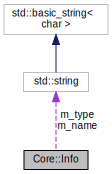
\includegraphics[width=175pt]{class_core_1_1_info__coll__graph}
\end{center}
\end{figure}


\subsection{Данные класса}
\index{Core\+::\+Info@{Core\+::\+Info}!m\+\_\+name@{m\+\_\+name}}
\index{m\+\_\+name@{m\+\_\+name}!Core\+::\+Info@{Core\+::\+Info}}
\subsubsection[{\texorpdfstring{m\+\_\+name}{m_name}}]{\setlength{\rightskip}{0pt plus 5cm}std\+::string Core\+::\+Info\+::m\+\_\+name\hspace{0.3cm}{\ttfamily [private]}}\hypertarget{class_core_1_1_info_a027464b5db2e89c6c2f48faf99d25b22}{}\label{class_core_1_1_info_a027464b5db2e89c6c2f48faf99d25b22}
Имя. 

См. определение в файле info.\+h строка 38

\index{Core\+::\+Info@{Core\+::\+Info}!m\+\_\+type@{m\+\_\+type}}
\index{m\+\_\+type@{m\+\_\+type}!Core\+::\+Info@{Core\+::\+Info}}
\subsubsection[{\texorpdfstring{m\+\_\+type}{m_type}}]{\setlength{\rightskip}{0pt plus 5cm}std\+::string Core\+::\+Info\+::m\+\_\+type\hspace{0.3cm}{\ttfamily [private]}}\hypertarget{class_core_1_1_info_aa5d089f59122826625d6dd68af47775e}{}\label{class_core_1_1_info_aa5d089f59122826625d6dd68af47775e}
Тип. 

См. определение в файле info.\+h строка 39



Объявления и описания членов классов находятся в файлах\+:\begin{DoxyCompactItemize}
\item 
src/core/info.\+h\item 
src/core/info.\+cc\end{DoxyCompactItemize}

\hypertarget{class_tasks_1_1_continuous_1_1_landing_gauss}{}\section{Класс Tasks\+:\+:Continuous\+:\+:Landing\+Gauss}
\label{class_tasks_1_1_continuous_1_1_landing_gauss}\index{Tasks\+::\+Continuous\+::\+Landing\+Gauss@{Tasks\+::\+Continuous\+::\+Landing\+Gauss}}
\subsection*{Дополнительные унаследованные члены}


\subsection{Подробное описание}


См. определение в файле c\+\_\+landing\+\_\+gauss.\+h строка 14



Граф наследования\+:Tasks\+:\+:Continuous\+:\+:Landing\+Gauss\+:
\nopagebreak
\begin{figure}[H]
\begin{center}
\leavevmode
\includegraphics[width=195pt]{class_tasks_1_1_continuous_1_1_landing_gauss__inherit__graph}
\end{center}
\end{figure}


Граф связей класса Tasks\+:\+:Continuous\+:\+:Landing\+Gauss\+:
\nopagebreak
\begin{figure}[H]
\begin{center}
\leavevmode
\includegraphics[width=328pt]{class_tasks_1_1_continuous_1_1_landing_gauss__coll__graph}
\end{center}
\end{figure}


Объявления и описания членов классов находятся в файлах\+:\begin{DoxyCompactItemize}
\item 
src/tasks/continuous/c\+\_\+landing\+\_\+gauss.\+h\item 
src/tasks/continuous/c\+\_\+landing\+\_\+gauss.\+cc\end{DoxyCompactItemize}

\hypertarget{class_tasks_1_1_continuous_discrete_1_1_landing_gauss}{}\section{Класс Tasks\+:\+:Continuous\+Discrete\+:\+:Landing\+Gauss}
\label{class_tasks_1_1_continuous_discrete_1_1_landing_gauss}\index{Tasks\+::\+Continuous\+Discrete\+::\+Landing\+Gauss@{Tasks\+::\+Continuous\+Discrete\+::\+Landing\+Gauss}}
\subsection*{Дополнительные унаследованные члены}


\subsection{Подробное описание}


См. определение в файле cd\+\_\+landing\+\_\+gauss.\+h строка 14



Граф наследования\+:Tasks\+:\+:Continuous\+Discrete\+:\+:Landing\+Gauss\+:
\nopagebreak
\begin{figure}[H]
\begin{center}
\leavevmode
\includegraphics[width=229pt]{class_tasks_1_1_continuous_discrete_1_1_landing_gauss__inherit__graph}
\end{center}
\end{figure}


Граф связей класса Tasks\+:\+:Continuous\+Discrete\+:\+:Landing\+Gauss\+:
\nopagebreak
\begin{figure}[H]
\begin{center}
\leavevmode
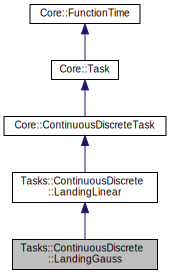
\includegraphics[width=229pt]{class_tasks_1_1_continuous_discrete_1_1_landing_gauss__coll__graph}
\end{center}
\end{figure}


Объявления и описания членов классов находятся в файлах\+:\begin{DoxyCompactItemize}
\item 
src/tasks/continuous\+\_\+discrete/cd\+\_\+landing\+\_\+gauss.\+h\item 
src/tasks/continuous\+\_\+discrete/cd\+\_\+landing\+\_\+gauss.\+cc\end{DoxyCompactItemize}

\hypertarget{class_tasks_1_1_discrete_1_1_landing_gauss}{}\section{Класс Tasks\+:\+:Discrete\+:\+:Landing\+Gauss}
\label{class_tasks_1_1_discrete_1_1_landing_gauss}\index{Tasks\+::\+Discrete\+::\+Landing\+Gauss@{Tasks\+::\+Discrete\+::\+Landing\+Gauss}}
\subsection*{Дополнительные унаследованные члены}


\subsection{Подробное описание}


См. определение в файле d\+\_\+landing\+\_\+gauss.\+h строка 14



Граф наследования\+:Tasks\+:\+:Discrete\+:\+:Landing\+Gauss\+:\nopagebreak
\begin{figure}[H]
\begin{center}
\leavevmode
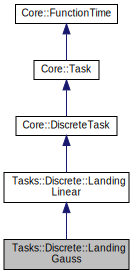
\includegraphics[width=214pt]{class_tasks_1_1_discrete_1_1_landing_gauss__inherit__graph}
\end{center}
\end{figure}


Граф связей класса Tasks\+:\+:Discrete\+:\+:Landing\+Gauss\+:\nopagebreak
\begin{figure}[H]
\begin{center}
\leavevmode
\includegraphics[width=214pt]{class_tasks_1_1_discrete_1_1_landing_gauss__coll__graph}
\end{center}
\end{figure}


Объявления и описания членов классов находятся в файлах\+:\begin{DoxyCompactItemize}
\item 
src/tasks/discrete/d\+\_\+landing\+\_\+gauss.\+h\item 
src/tasks/discrete/d\+\_\+landing\+\_\+gauss.\+cc\end{DoxyCompactItemize}

\hypertarget{class_tasks_1_1_continuous_1_1_landing_linear}{}\section{Класс Tasks\+:\+:Continuous\+:\+:Landing\+Linear}
\label{class_tasks_1_1_continuous_1_1_landing_linear}\index{Tasks\+::\+Continuous\+::\+Landing\+Linear@{Tasks\+::\+Continuous\+::\+Landing\+Linear}}


Задача спуска ЛА на планету (непрерывная, линеаризованная) для фильтров оптимальной структуры.  




{\ttfamily \#include \char`\"{}c\+\_\+landing\+\_\+linear.\+h\char`\"{}}

\subsection*{Открытые члены}
\begin{DoxyCompactItemize}
\item 
\hyperlink{class_tasks_1_1_continuous_1_1_landing_linear_a29e44f6089f6ff4ef86bfcacdaefa3fd}{Landing\+Linear} ()\hypertarget{class_tasks_1_1_continuous_1_1_landing_linear_a29e44f6089f6ff4ef86bfcacdaefa3fd}{}\label{class_tasks_1_1_continuous_1_1_landing_linear_a29e44f6089f6ff4ef86bfcacdaefa3fd}

\begin{DoxyCompactList}\small\item\em Конструктор. \end{DoxyCompactList}\item 
Vector \hyperlink{class_tasks_1_1_continuous_1_1_landing_linear_a610d7e38cb0ab74bd197ab45d82e5df6}{a} (const Vector \&x) const override\hypertarget{class_tasks_1_1_continuous_1_1_landing_linear_a610d7e38cb0ab74bd197ab45d82e5df6}{}\label{class_tasks_1_1_continuous_1_1_landing_linear_a610d7e38cb0ab74bd197ab45d82e5df6}

\begin{DoxyCompactList}\small\item\em Функция сноса объекта $a(t,x)$. \end{DoxyCompactList}\item 
Matrix \hyperlink{class_tasks_1_1_continuous_1_1_landing_linear_a65f50434686453de5d976699055075dd}{B} (const Vector \&x) const override\hypertarget{class_tasks_1_1_continuous_1_1_landing_linear_a65f50434686453de5d976699055075dd}{}\label{class_tasks_1_1_continuous_1_1_landing_linear_a65f50434686453de5d976699055075dd}

\begin{DoxyCompactList}\small\item\em Функция диффузии объекта $B(t,x)$. \end{DoxyCompactList}\item 
Vector \hyperlink{class_tasks_1_1_continuous_1_1_landing_linear_af180804a46299b6d7128dce0bff6c91a}{c} (const Vector \&x) const override\hypertarget{class_tasks_1_1_continuous_1_1_landing_linear_af180804a46299b6d7128dce0bff6c91a}{}\label{class_tasks_1_1_continuous_1_1_landing_linear_af180804a46299b6d7128dce0bff6c91a}

\begin{DoxyCompactList}\small\item\em Функция сноса измерителя $с(t,x)$. \end{DoxyCompactList}\item 
Matrix \hyperlink{class_tasks_1_1_continuous_1_1_landing_linear_a829c4b67c6a4cd8bb1a430e4e55d9d45}{D} (const Vector \&x) const override\hypertarget{class_tasks_1_1_continuous_1_1_landing_linear_a829c4b67c6a4cd8bb1a430e4e55d9d45}{}\label{class_tasks_1_1_continuous_1_1_landing_linear_a829c4b67c6a4cd8bb1a430e4e55d9d45}

\begin{DoxyCompactList}\small\item\em Функция диффузии измерителя $D(t,x)$. \end{DoxyCompactList}\item 
Matrix \hyperlink{class_tasks_1_1_continuous_1_1_landing_linear_a8b06d0f38d73a27f7de0df6ba36b9c38}{A} (const Vector \&m, const Matrix \&\hyperlink{class_tasks_1_1_continuous_1_1_landing_linear_a829c4b67c6a4cd8bb1a430e4e55d9d45}{D}) const override
\begin{DoxyCompactList}\small\item\em Структурная функция $A(t, m, D)$. \end{DoxyCompactList}\item 
Matrix \hyperlink{class_tasks_1_1_continuous_1_1_landing_linear_af5937be9d9010e853956e5dd7ff96e8d}{G} (const Vector \&m, const Matrix \&\hyperlink{class_tasks_1_1_continuous_1_1_landing_linear_a829c4b67c6a4cd8bb1a430e4e55d9d45}{D}) const override
\begin{DoxyCompactList}\small\item\em Структурная функция $G(t, m, D)$. \end{DoxyCompactList}\end{DoxyCompactItemize}
\subsection*{Защищенные члены}
\begin{DoxyCompactItemize}
\item 
Matrix \hyperlink{class_tasks_1_1_continuous_1_1_landing_linear_a95641c126ba2e99da83cd6f3683b6238}{Q} (const Vector \&m, const Matrix \&\hyperlink{class_tasks_1_1_continuous_1_1_landing_linear_a829c4b67c6a4cd8bb1a430e4e55d9d45}{D}) const override\hypertarget{class_tasks_1_1_continuous_1_1_landing_linear_a95641c126ba2e99da83cd6f3683b6238}{}\label{class_tasks_1_1_continuous_1_1_landing_linear_a95641c126ba2e99da83cd6f3683b6238}

\begin{DoxyCompactList}\small\item\em Возвращает интенсивность шумов $Q(\cdot) = B(\cdot) \cdot B^T(\cdot)$. \end{DoxyCompactList}\item 
Matrix \hyperlink{class_tasks_1_1_continuous_1_1_landing_linear_a886bc6dd08e4355ab0c491d48f9de002}{S} (const Vector \&m, const Matrix \&\hyperlink{class_tasks_1_1_continuous_1_1_landing_linear_a829c4b67c6a4cd8bb1a430e4e55d9d45}{D}) const override
\begin{DoxyCompactList}\small\item\em Возвращает интенсивность шумов $S(\cdot) = B(\cdot) \cdot D^T(\cdot)$. \end{DoxyCompactList}\item 
Matrix \hyperlink{class_tasks_1_1_continuous_1_1_landing_linear_a1eaa8243f547b6cbd3b29ec625f887a8}{R} (const Vector \&m, const Matrix \&\hyperlink{class_tasks_1_1_continuous_1_1_landing_linear_a829c4b67c6a4cd8bb1a430e4e55d9d45}{D}) const override\hypertarget{class_tasks_1_1_continuous_1_1_landing_linear_a1eaa8243f547b6cbd3b29ec625f887a8}{}\label{class_tasks_1_1_continuous_1_1_landing_linear_a1eaa8243f547b6cbd3b29ec625f887a8}

\begin{DoxyCompactList}\small\item\em Возвращает интенсивность шумов $R(\cdot) = D(\cdot) \cdot D^T(\cdot)$. \end{DoxyCompactList}\item 
void \hyperlink{class_tasks_1_1_continuous_1_1_landing_linear_ac860d39de1972d7484ac665d174b0b94}{load\+Params} () override\hypertarget{class_tasks_1_1_continuous_1_1_landing_linear_ac860d39de1972d7484ac665d174b0b94}{}\label{class_tasks_1_1_continuous_1_1_landing_linear_ac860d39de1972d7484ac665d174b0b94}

\begin{DoxyCompactList}\small\item\em Загружает данные в локальные переменные после изменения параметров. \end{DoxyCompactList}\item 
double {\bfseries k} (double t) const \hypertarget{class_tasks_1_1_continuous_1_1_landing_linear_ac1ca1187944b2a44adbf486cc7c72d4c}{}\label{class_tasks_1_1_continuous_1_1_landing_linear_ac1ca1187944b2a44adbf486cc7c72d4c}

\end{DoxyCompactItemize}
\subsection*{Защищенные данные}
\begin{DoxyCompactItemize}
\item 
double {\bfseries m\+\_\+turn\+Time}\hypertarget{class_tasks_1_1_continuous_1_1_landing_linear_a79bc6b7e7f836080684aa36e4f6cec5f}{}\label{class_tasks_1_1_continuous_1_1_landing_linear_a79bc6b7e7f836080684aa36e4f6cec5f}

\end{DoxyCompactItemize}
\subsection*{Статические защищенные данные}
\begin{DoxyCompactItemize}
\item 
static constexpr double {\bfseries KB} = 0.\+3\hypertarget{class_tasks_1_1_continuous_1_1_landing_linear_a429e2f85bd502a35b59f84021f63e456}{}\label{class_tasks_1_1_continuous_1_1_landing_linear_a429e2f85bd502a35b59f84021f63e456}

\item 
static constexpr double {\bfseries BB} = 0.\+09\hypertarget{class_tasks_1_1_continuous_1_1_landing_linear_a9327ad0f9f6f06ce3278722f42d4cc42}{}\label{class_tasks_1_1_continuous_1_1_landing_linear_a9327ad0f9f6f06ce3278722f42d4cc42}

\item 
static constexpr double {\bfseries CC} = 0.\+043333333333333333333333333333333333333333333333333\hypertarget{class_tasks_1_1_continuous_1_1_landing_linear_ab539ba664a08722ed6c9a855be340567}{}\label{class_tasks_1_1_continuous_1_1_landing_linear_ab539ba664a08722ed6c9a855be340567}

\item 
static constexpr double {\bfseries GG} = 3.\+711\+E-\/3\hypertarget{class_tasks_1_1_continuous_1_1_landing_linear_a9a79b7472c9e491554ca0f76b76106e0}{}\label{class_tasks_1_1_continuous_1_1_landing_linear_a9a79b7472c9e491554ca0f76b76106e0}

\item 
static constexpr double {\bfseries RR} = 3390.\+0\hypertarget{class_tasks_1_1_continuous_1_1_landing_linear_ae35b8a06f6479415f11e967602fbf0d6}{}\label{class_tasks_1_1_continuous_1_1_landing_linear_ae35b8a06f6479415f11e967602fbf0d6}

\end{DoxyCompactItemize}


\subsection{Подробное описание}
Задача спуска ЛА на планету (непрерывная, линеаризованная) для фильтров оптимальной структуры. 

См. определение в файле c\+\_\+landing\+\_\+linear.\+h строка 20



Граф наследования\+:Tasks\+:\+:Continuous\+:\+:Landing\+Linear\+:
\nopagebreak
\begin{figure}[H]
\begin{center}
\leavevmode
\includegraphics[width=195pt]{class_tasks_1_1_continuous_1_1_landing_linear__inherit__graph}
\end{center}
\end{figure}


Граф связей класса Tasks\+:\+:Continuous\+:\+:Landing\+Linear\+:
\nopagebreak
\begin{figure}[H]
\begin{center}
\leavevmode
\includegraphics[width=328pt]{class_tasks_1_1_continuous_1_1_landing_linear__coll__graph}
\end{center}
\end{figure}


\subsection{Методы}
\index{Tasks\+::\+Continuous\+::\+Landing\+Linear@{Tasks\+::\+Continuous\+::\+Landing\+Linear}!A@{A}}
\index{A@{A}!Tasks\+::\+Continuous\+::\+Landing\+Linear@{Tasks\+::\+Continuous\+::\+Landing\+Linear}}
\subsubsection[{\texorpdfstring{A(const Vector \&m, const Matrix \&\+D) const override}{A(const Vector &m, const Matrix &D) const override}}]{\setlength{\rightskip}{0pt plus 5cm}Matrix Tasks\+::\+Continuous\+::\+Landing\+Linear\+::A (
\begin{DoxyParamCaption}
\item[{const Vector \&}]{m, }
\item[{const Matrix \&}]{D}
\end{DoxyParamCaption}
) const\hspace{0.3cm}{\ttfamily [override]}, {\ttfamily [virtual]}}\hypertarget{class_tasks_1_1_continuous_1_1_landing_linear_a8b06d0f38d73a27f7de0df6ba36b9c38}{}\label{class_tasks_1_1_continuous_1_1_landing_linear_a8b06d0f38d73a27f7de0df6ba36b9c38}


Структурная функция $A(t, m, D)$. 

Она имеет следующий вид для


\begin{DoxyItemize}
\item линеаризованного приближения\+: \[A(t, m, D) = \frac{d}{dm} a(t, m).\] 
\end{DoxyItemize}

Замещает \hyperlink{class_core_1_1_continuous_task_a75fbac1abe67223cd7938b724c5cce45}{Core\+::\+Continuous\+Task}.



См. определение в файле c\+\_\+landing\+\_\+linear.\+cc строка 128

\index{Tasks\+::\+Continuous\+::\+Landing\+Linear@{Tasks\+::\+Continuous\+::\+Landing\+Linear}!G@{G}}
\index{G@{G}!Tasks\+::\+Continuous\+::\+Landing\+Linear@{Tasks\+::\+Continuous\+::\+Landing\+Linear}}
\subsubsection[{\texorpdfstring{G(const Vector \&m, const Matrix \&\+D) const override}{G(const Vector &m, const Matrix &D) const override}}]{\setlength{\rightskip}{0pt plus 5cm}Matrix Tasks\+::\+Continuous\+::\+Landing\+Linear\+::G (
\begin{DoxyParamCaption}
\item[{const Vector \&}]{m, }
\item[{const Matrix \&}]{D}
\end{DoxyParamCaption}
) const\hspace{0.3cm}{\ttfamily [override]}, {\ttfamily [virtual]}}\hypertarget{class_tasks_1_1_continuous_1_1_landing_linear_af5937be9d9010e853956e5dd7ff96e8d}{}\label{class_tasks_1_1_continuous_1_1_landing_linear_af5937be9d9010e853956e5dd7ff96e8d}


Структурная функция $G(t, m, D)$. 

Она имеет следующий вид для


\begin{DoxyItemize}
\item линеаризованного приближения\+: \[G(t, m, D) = \frac{d}{dm} c(t, m).\] 
\end{DoxyItemize}

Замещает \hyperlink{class_core_1_1_continuous_task_a1b579e183ffa229f97048aadfd834517}{Core\+::\+Continuous\+Task}.



См. определение в файле c\+\_\+landing\+\_\+linear.\+cc строка 148

\index{Tasks\+::\+Continuous\+::\+Landing\+Linear@{Tasks\+::\+Continuous\+::\+Landing\+Linear}!S@{S}}
\index{S@{S}!Tasks\+::\+Continuous\+::\+Landing\+Linear@{Tasks\+::\+Continuous\+::\+Landing\+Linear}}
\subsubsection[{\texorpdfstring{S(const Vector \&m, const Matrix \&\+D) const override}{S(const Vector &m, const Matrix &D) const override}}]{\setlength{\rightskip}{0pt plus 5cm}Matrix Tasks\+::\+Continuous\+::\+Landing\+Linear\+::S (
\begin{DoxyParamCaption}
\item[{const Vector \&}]{m, }
\item[{const Matrix \&}]{D}
\end{DoxyParamCaption}
) const\hspace{0.3cm}{\ttfamily [override]}, {\ttfamily [protected]}, {\ttfamily [virtual]}}\hypertarget{class_tasks_1_1_continuous_1_1_landing_linear_a886bc6dd08e4355ab0c491d48f9de002}{}\label{class_tasks_1_1_continuous_1_1_landing_linear_a886bc6dd08e4355ab0c491d48f9de002}


Возвращает интенсивность шумов $S(\cdot) = B(\cdot) \cdot D^T(\cdot)$. 

\begin{DoxyWarning}{Предупреждения}
Так как шумы независимые, то должна возвращать нулевую матрицу (нулевая взаимная интенсивность). 
\end{DoxyWarning}


Замещает \hyperlink{class_core_1_1_continuous_task_aa6d652b655628586aeeda03348f633c5}{Core\+::\+Continuous\+Task}.



См. определение в файле c\+\_\+landing\+\_\+linear.\+cc строка 116



Объявления и описания членов классов находятся в файлах\+:\begin{DoxyCompactItemize}
\item 
src/tasks/continuous/c\+\_\+landing\+\_\+linear.\+h\item 
src/tasks/continuous/c\+\_\+landing\+\_\+linear.\+cc\end{DoxyCompactItemize}

\hypertarget{class_tasks_1_1_discrete_1_1_landing_linear}{}\section{Класс Tasks\+:\+:Discrete\+:\+:Landing\+Linear}
\label{class_tasks_1_1_discrete_1_1_landing_linear}\index{Tasks\+::\+Discrete\+::\+Landing\+Linear@{Tasks\+::\+Discrete\+::\+Landing\+Linear}}


Задача спуска ЛА на планету (дискретная, линеаризованная) для фильтров оптимальной структуры.  




{\ttfamily \#include \char`\"{}d\+\_\+landing\+\_\+linear.\+h\char`\"{}}

\subsection*{Открытые члены}
\begin{DoxyCompactItemize}
\item 
\hypertarget{class_tasks_1_1_discrete_1_1_landing_linear_a635a395c8b9ef9bcece3201c26c258bf}{}\label{class_tasks_1_1_discrete_1_1_landing_linear_a635a395c8b9ef9bcece3201c26c258bf} 
\hyperlink{class_tasks_1_1_discrete_1_1_landing_linear_a635a395c8b9ef9bcece3201c26c258bf}{Landing\+Linear} ()
\begin{DoxyCompactList}\small\item\em Конструктор. \end{DoxyCompactList}\item 
Vector \hyperlink{class_tasks_1_1_discrete_1_1_landing_linear_af0c0c48603fc226055ee233f93fa21fc}{a} (const Vector \&x) const override
\begin{DoxyCompactList}\small\item\em Функция объекта $a_k(X_k) = a_k(X_k, V_k)$. \end{DoxyCompactList}\item 
Vector \hyperlink{class_tasks_1_1_discrete_1_1_landing_linear_a599d3491da6d84ba68c43433235e9980}{b} (const Vector \&x) const override
\begin{DoxyCompactList}\small\item\em Функция измерителя $b(X_k) = b_k(X_k, W_k)$. \end{DoxyCompactList}\item 
Vector \hyperlink{class_tasks_1_1_discrete_1_1_landing_linear_a8f2022967fae3dde3e7d2df3f7fa98f8}{tau} (const Vector \&z, const Matrix \&P) const override
\begin{DoxyCompactList}\small\item\em Структурная функция прогноза $\tau_k(m, D)$. \end{DoxyCompactList}\item 
Matrix \hyperlink{class_tasks_1_1_discrete_1_1_landing_linear_a88dda707914dea5698748f445563400f}{Theta} (const Vector \&z, const Matrix \&P) const override
\begin{DoxyCompactList}\small\item\em Структурная функция прогноза $\Theta_k(m, D)$. \end{DoxyCompactList}\item 
Vector \hyperlink{class_tasks_1_1_discrete_1_1_landing_linear_a9b1f90547fca3b460b48693b2e16219a}{h} (const Vector \&m, const Matrix \&D) const override
\begin{DoxyCompactList}\small\item\em Структурная функция коррекции $h_k(m, D)$. \end{DoxyCompactList}\item 
Matrix \hyperlink{class_tasks_1_1_discrete_1_1_landing_linear_a290890c1d3a91803249a1f5d62bc658f}{G} (const Vector \&m, const Matrix \&D) const override
\begin{DoxyCompactList}\small\item\em Структурная функция коррекции $G_k(m, D)$. \end{DoxyCompactList}\item 
Matrix \hyperlink{class_tasks_1_1_discrete_1_1_landing_linear_abb4e2b054240cf909f0128721237334c}{F} (const Vector \&m, const Matrix \&D) const override
\begin{DoxyCompactList}\small\item\em Структурная функция коррекции $F_k(m, D)$. \end{DoxyCompactList}\end{DoxyCompactItemize}
\subsection*{Защищенные члены}
\begin{DoxyCompactItemize}
\item 
\hypertarget{class_tasks_1_1_discrete_1_1_landing_linear_a8d1a37601f2184254e8ff8f97e026756}{}\label{class_tasks_1_1_discrete_1_1_landing_linear_a8d1a37601f2184254e8ff8f97e026756} 
Matrix \hyperlink{class_tasks_1_1_discrete_1_1_landing_linear_a8d1a37601f2184254e8ff8f97e026756}{dadx} (const Vector \&x) const override
\begin{DoxyCompactList}\small\item\em Вспомогательная функция, вычисляет $\nabla_x a_k(x,v)$. \end{DoxyCompactList}\item 
\hypertarget{class_tasks_1_1_discrete_1_1_landing_linear_aa72d305c7731e8972d99c04ef034ee22}{}\label{class_tasks_1_1_discrete_1_1_landing_linear_aa72d305c7731e8972d99c04ef034ee22} 
Matrix \hyperlink{class_tasks_1_1_discrete_1_1_landing_linear_aa72d305c7731e8972d99c04ef034ee22}{dadv} (const Vector \&x) const override
\begin{DoxyCompactList}\small\item\em Вспомогательная функция, вычисляет $\nabla_v a_k(x,v)$. \end{DoxyCompactList}\item 
\hypertarget{class_tasks_1_1_discrete_1_1_landing_linear_a7db5ae69d850f20d01efd665906b5b83}{}\label{class_tasks_1_1_discrete_1_1_landing_linear_a7db5ae69d850f20d01efd665906b5b83} 
Matrix \hyperlink{class_tasks_1_1_discrete_1_1_landing_linear_a7db5ae69d850f20d01efd665906b5b83}{dbdx} (const Vector \&x) const override
\begin{DoxyCompactList}\small\item\em Вспомогательная функция, вычисляет $\nabla_x b_k(x,w)$. \end{DoxyCompactList}\item 
\hypertarget{class_tasks_1_1_discrete_1_1_landing_linear_a25be613741f960811d693852d230a3eb}{}\label{class_tasks_1_1_discrete_1_1_landing_linear_a25be613741f960811d693852d230a3eb} 
Matrix \hyperlink{class_tasks_1_1_discrete_1_1_landing_linear_a25be613741f960811d693852d230a3eb}{dbdw} (const Vector \&x) const override
\begin{DoxyCompactList}\small\item\em Вспомогательная функция, вычисляет $\nabla_w b_k(x,w)$. \end{DoxyCompactList}\item 
\hypertarget{class_tasks_1_1_discrete_1_1_landing_linear_a955c4de6dbe0a71bc97d0bf39f695054}{}\label{class_tasks_1_1_discrete_1_1_landing_linear_a955c4de6dbe0a71bc97d0bf39f695054} 
void \hyperlink{class_tasks_1_1_discrete_1_1_landing_linear_a955c4de6dbe0a71bc97d0bf39f695054}{load\+Params} () override
\begin{DoxyCompactList}\small\item\em Загружает данные в локальные переменные после изменения параметров. \end{DoxyCompactList}\item 
\hypertarget{class_tasks_1_1_discrete_1_1_landing_linear_a8e641e61f366d3f4145a9b0c3b53b37e}{}\label{class_tasks_1_1_discrete_1_1_landing_linear_a8e641e61f366d3f4145a9b0c3b53b37e} 
double {\bfseries k} (double t) const
\end{DoxyCompactItemize}
\subsection*{Защищенные данные}
\begin{DoxyCompactItemize}
\item 
\hypertarget{class_tasks_1_1_discrete_1_1_landing_linear_a95cd1d6b8774484348cf21842bc1ab82}{}\label{class_tasks_1_1_discrete_1_1_landing_linear_a95cd1d6b8774484348cf21842bc1ab82} 
double {\bfseries m\+\_\+turn\+Time}
\end{DoxyCompactItemize}
\subsection*{Статические защищенные данные}
\begin{DoxyCompactItemize}
\item 
\hypertarget{class_tasks_1_1_discrete_1_1_landing_linear_ab62185db94c68bc2ea5449b455b71ca9}{}\label{class_tasks_1_1_discrete_1_1_landing_linear_ab62185db94c68bc2ea5449b455b71ca9} 
static constexpr double {\bfseries KB} = 0.\+3
\item 
\hypertarget{class_tasks_1_1_discrete_1_1_landing_linear_a27e46b3c8f6359b7fe37205fe6d4b009}{}\label{class_tasks_1_1_discrete_1_1_landing_linear_a27e46b3c8f6359b7fe37205fe6d4b009} 
static constexpr double {\bfseries BB} = 0.\+09
\item 
\hypertarget{class_tasks_1_1_discrete_1_1_landing_linear_ae2d5423e0cc942b236f97b55d16070b2}{}\label{class_tasks_1_1_discrete_1_1_landing_linear_ae2d5423e0cc942b236f97b55d16070b2} 
static constexpr double {\bfseries CC} = 0.\+043333333333333333333333333333333333333333333333333
\item 
\hypertarget{class_tasks_1_1_discrete_1_1_landing_linear_a54a6e7e6668dae1ba3e700f633031b34}{}\label{class_tasks_1_1_discrete_1_1_landing_linear_a54a6e7e6668dae1ba3e700f633031b34} 
static constexpr double {\bfseries GG} = 3.\+711\+E-\/3
\item 
\hypertarget{class_tasks_1_1_discrete_1_1_landing_linear_a5de434a509158bf23cb5fba7445b2e2d}{}\label{class_tasks_1_1_discrete_1_1_landing_linear_a5de434a509158bf23cb5fba7445b2e2d} 
static constexpr double {\bfseries RR} = 3390.\+0
\end{DoxyCompactItemize}


\subsection{Подробное описание}
Задача спуска ЛА на планету (дискретная, линеаризованная) для фильтров оптимальной структуры. 

См. определение в файле d\+\_\+landing\+\_\+linear.\+h строка 21



Граф наследования\+:Tasks\+:\+:Discrete\+:\+:Landing\+Linear\+:\nopagebreak
\begin{figure}[H]
\begin{center}
\leavevmode
\includegraphics[width=214pt]{class_tasks_1_1_discrete_1_1_landing_linear__inherit__graph}
\end{center}
\end{figure}


Граф связей класса Tasks\+:\+:Discrete\+:\+:Landing\+Linear\+:\nopagebreak
\begin{figure}[H]
\begin{center}
\leavevmode
\includegraphics[width=214pt]{class_tasks_1_1_discrete_1_1_landing_linear__coll__graph}
\end{center}
\end{figure}


\subsection{Методы}
\hypertarget{class_tasks_1_1_discrete_1_1_landing_linear_af0c0c48603fc226055ee233f93fa21fc}{}\label{class_tasks_1_1_discrete_1_1_landing_linear_af0c0c48603fc226055ee233f93fa21fc} 
\index{Tasks\+::\+Discrete\+::\+Landing\+Linear@{Tasks\+::\+Discrete\+::\+Landing\+Linear}!a@{a}}
\index{a@{a}!Tasks\+::\+Discrete\+::\+Landing\+Linear@{Tasks\+::\+Discrete\+::\+Landing\+Linear}}
\subsubsection{\texorpdfstring{a()}{a()}}
{\footnotesize\ttfamily Vector Tasks\+::\+Discrete\+::\+Landing\+Linear\+::a (\begin{DoxyParamCaption}\item[{const Vector \&}]{x }\end{DoxyParamCaption}) const\hspace{0.3cm}{\ttfamily [override]}, {\ttfamily [virtual]}}



Функция объекта $a_k(X_k) = a_k(X_k, V_k)$. 

Шум $V_k$ генерируется внутри. 

Замещает \hyperlink{class_core_1_1_discrete_task_a49d377fa365d5ec3e05962ee751f2d9e}{Core\+::\+Discrete\+Task}.



См. определение в файле d\+\_\+landing\+\_\+linear.\+cc строка 69

\hypertarget{class_tasks_1_1_discrete_1_1_landing_linear_a599d3491da6d84ba68c43433235e9980}{}\label{class_tasks_1_1_discrete_1_1_landing_linear_a599d3491da6d84ba68c43433235e9980} 
\index{Tasks\+::\+Discrete\+::\+Landing\+Linear@{Tasks\+::\+Discrete\+::\+Landing\+Linear}!b@{b}}
\index{b@{b}!Tasks\+::\+Discrete\+::\+Landing\+Linear@{Tasks\+::\+Discrete\+::\+Landing\+Linear}}
\subsubsection{\texorpdfstring{b()}{b()}}
{\footnotesize\ttfamily Vector Tasks\+::\+Discrete\+::\+Landing\+Linear\+::b (\begin{DoxyParamCaption}\item[{const Vector \&}]{x }\end{DoxyParamCaption}) const\hspace{0.3cm}{\ttfamily [override]}, {\ttfamily [virtual]}}



Функция измерителя $b(X_k) = b_k(X_k, W_k)$. 

Шум $W_k$ генерируется внутри. 

Замещает \hyperlink{class_core_1_1_discrete_task_a82c1aa8100dd9211739f8fd9f7d52c81}{Core\+::\+Discrete\+Task}.



См. определение в файле d\+\_\+landing\+\_\+linear.\+cc строка 81

\hypertarget{class_tasks_1_1_discrete_1_1_landing_linear_abb4e2b054240cf909f0128721237334c}{}\label{class_tasks_1_1_discrete_1_1_landing_linear_abb4e2b054240cf909f0128721237334c} 
\index{Tasks\+::\+Discrete\+::\+Landing\+Linear@{Tasks\+::\+Discrete\+::\+Landing\+Linear}!F@{F}}
\index{F@{F}!Tasks\+::\+Discrete\+::\+Landing\+Linear@{Tasks\+::\+Discrete\+::\+Landing\+Linear}}
\subsubsection{\texorpdfstring{F()}{F()}}
{\footnotesize\ttfamily Matrix Tasks\+::\+Discrete\+::\+Landing\+Linear\+::F (\begin{DoxyParamCaption}\item[{const Vector \&}]{m,  }\item[{const Matrix \&}]{D }\end{DoxyParamCaption}) const\hspace{0.3cm}{\ttfamily [override]}, {\ttfamily [virtual]}}



Структурная функция коррекции $F_k(m, D)$. 

Она имеет следующий вид для


\begin{DoxyItemize}
\item гауссовского приближения\+: \[F_k(m, D) = M_N[M[b_k(m, W_k)\cdot b_k^T(m, W_k)] \ |\ m, D] - h_k(m,D) \cdot h_k^T(m, D),\]
\item линеаризованного приближения\+: \[F_k(m, D) = B_k^x(m) \cdot D \cdot B_k^{xT}(m) + B_k^w(m) \cdot D[W_k] \cdot B_k^{wT}(m).\]
\end{DoxyItemize}

Здесь $B_k^x(x) = \nabla_x b_k(x, M[W_k]),\ B_k^w(x) = \nabla_w b_k(x, M[W_k])$. 

Замещает \hyperlink{class_core_1_1_discrete_task_ac55ca2cd47f0c9f7e5d3d3704becee46}{Core\+::\+Discrete\+Task}.



См. определение в файле d\+\_\+landing\+\_\+linear.\+cc строка 124

\hypertarget{class_tasks_1_1_discrete_1_1_landing_linear_a290890c1d3a91803249a1f5d62bc658f}{}\label{class_tasks_1_1_discrete_1_1_landing_linear_a290890c1d3a91803249a1f5d62bc658f} 
\index{Tasks\+::\+Discrete\+::\+Landing\+Linear@{Tasks\+::\+Discrete\+::\+Landing\+Linear}!G@{G}}
\index{G@{G}!Tasks\+::\+Discrete\+::\+Landing\+Linear@{Tasks\+::\+Discrete\+::\+Landing\+Linear}}
\subsubsection{\texorpdfstring{G()}{G()}}
{\footnotesize\ttfamily Matrix Tasks\+::\+Discrete\+::\+Landing\+Linear\+::G (\begin{DoxyParamCaption}\item[{const Vector \&}]{m,  }\item[{const Matrix \&}]{D }\end{DoxyParamCaption}) const\hspace{0.3cm}{\ttfamily [override]}, {\ttfamily [virtual]}}



Структурная функция коррекции $G_k(m, D)$. 

Она имеет следующий вид для


\begin{DoxyItemize}
\item гауссовского приближения\+: \[G_k(m, D) = \nabla_m h_k(m,D),\]
\item линеаризованного приближения\+: \[G_k(m, D) = \nabla_m b_k(m, M[W_k]).\] 
\end{DoxyItemize}

Замещает \hyperlink{class_core_1_1_discrete_task_a5fd0bac544a6e124ad071043a37881c3}{Core\+::\+Discrete\+Task}.



См. определение в файле d\+\_\+landing\+\_\+linear.\+cc строка 119

\hypertarget{class_tasks_1_1_discrete_1_1_landing_linear_a9b1f90547fca3b460b48693b2e16219a}{}\label{class_tasks_1_1_discrete_1_1_landing_linear_a9b1f90547fca3b460b48693b2e16219a} 
\index{Tasks\+::\+Discrete\+::\+Landing\+Linear@{Tasks\+::\+Discrete\+::\+Landing\+Linear}!h@{h}}
\index{h@{h}!Tasks\+::\+Discrete\+::\+Landing\+Linear@{Tasks\+::\+Discrete\+::\+Landing\+Linear}}
\subsubsection{\texorpdfstring{h()}{h()}}
{\footnotesize\ttfamily Vector Tasks\+::\+Discrete\+::\+Landing\+Linear\+::h (\begin{DoxyParamCaption}\item[{const Vector \&}]{m,  }\item[{const Matrix \&}]{D }\end{DoxyParamCaption}) const\hspace{0.3cm}{\ttfamily [override]}, {\ttfamily [virtual]}}



Структурная функция коррекции $h_k(m, D)$. 

Она имеет следующий вид для


\begin{DoxyItemize}
\item гауссовского приближения\+: \[h_k(m, D) = M_N[M[b_k(m, W_k)] \ |\ m, D],\]
\item линеаризованного приближения\+: \[h_k(m, D) = b_k(m, M[W_k]).\] 
\end{DoxyItemize}

Замещает \hyperlink{class_core_1_1_discrete_task_a09eb964bfe445c1905758bfff4fc1537}{Core\+::\+Discrete\+Task}.



См. определение в файле d\+\_\+landing\+\_\+linear.\+cc строка 108

\hypertarget{class_tasks_1_1_discrete_1_1_landing_linear_a8f2022967fae3dde3e7d2df3f7fa98f8}{}\label{class_tasks_1_1_discrete_1_1_landing_linear_a8f2022967fae3dde3e7d2df3f7fa98f8} 
\index{Tasks\+::\+Discrete\+::\+Landing\+Linear@{Tasks\+::\+Discrete\+::\+Landing\+Linear}!tau@{tau}}
\index{tau@{tau}!Tasks\+::\+Discrete\+::\+Landing\+Linear@{Tasks\+::\+Discrete\+::\+Landing\+Linear}}
\subsubsection{\texorpdfstring{tau()}{tau()}}
{\footnotesize\ttfamily Vector Tasks\+::\+Discrete\+::\+Landing\+Linear\+::tau (\begin{DoxyParamCaption}\item[{const Vector \&}]{m,  }\item[{const Matrix \&}]{D }\end{DoxyParamCaption}) const\hspace{0.3cm}{\ttfamily [override]}, {\ttfamily [virtual]}}



Структурная функция прогноза $\tau_k(m, D)$. 

Она имеет следующий вид для


\begin{DoxyItemize}
\item гауссовского приближения\+: \[\tau_k(m, D) = M_N[M[a_k(m, V_k)] \ |\ m, D],\]
\item линеаризованного приближения\+: \[\tau_k(m, D) = a_k(m, M[V_k]).\] 
\end{DoxyItemize}

Замещает \hyperlink{class_core_1_1_discrete_task_aed780d7286bc88d0a2debb585601b3ca}{Core\+::\+Discrete\+Task}.



См. определение в файле d\+\_\+landing\+\_\+linear.\+cc строка 93

\hypertarget{class_tasks_1_1_discrete_1_1_landing_linear_a88dda707914dea5698748f445563400f}{}\label{class_tasks_1_1_discrete_1_1_landing_linear_a88dda707914dea5698748f445563400f} 
\index{Tasks\+::\+Discrete\+::\+Landing\+Linear@{Tasks\+::\+Discrete\+::\+Landing\+Linear}!Theta@{Theta}}
\index{Theta@{Theta}!Tasks\+::\+Discrete\+::\+Landing\+Linear@{Tasks\+::\+Discrete\+::\+Landing\+Linear}}
\subsubsection{\texorpdfstring{Theta()}{Theta()}}
{\footnotesize\ttfamily Matrix Tasks\+::\+Discrete\+::\+Landing\+Linear\+::\+Theta (\begin{DoxyParamCaption}\item[{const Vector \&}]{m,  }\item[{const Matrix \&}]{D }\end{DoxyParamCaption}) const\hspace{0.3cm}{\ttfamily [override]}, {\ttfamily [virtual]}}



Структурная функция прогноза $\Theta_k(m, D)$. 

Она имеет следующий вид для


\begin{DoxyItemize}
\item гауссовского приближения\+: \[\Theta_k(m, D) = M_N[M[a_k(m, V_k)\cdot a_k^T(m, V_k)]\ |\ m, D] - \tau_k(m,D) \cdot \tau_k^T(m, D),\]
\item линеаризованного приближения\+: \[\Theta_k(m, D) = A_k^x(m) \cdot D \cdot A_k^{xT}(m) + A_k^v(m) \cdot D[V_k] \cdot A_k^{v T}(m)\]
\end{DoxyItemize}

Здесь $A_k^x(x) = \nabla_x a_k(x,M[V_k]),\ A_k^v(x) = \nabla_v a_k(x,M[V_k])$. 

Замещает \hyperlink{class_core_1_1_discrete_task_a18906155257c5febd937f2f0c633e5ed}{Core\+::\+Discrete\+Task}.



См. определение в файле d\+\_\+landing\+\_\+linear.\+cc строка 98



Объявления и описания членов классов находятся в файлах\+:\begin{DoxyCompactItemize}
\item 
src/tasks/discrete/d\+\_\+landing\+\_\+linear.\+h\item 
src/tasks/discrete/d\+\_\+landing\+\_\+linear.\+cc\end{DoxyCompactItemize}

\hypertarget{class_tasks_1_1_continuous_discrete_1_1_landing_linear}{}\section{Класс Tasks\+:\+:Continuous\+Discrete\+:\+:Landing\+Linear}
\label{class_tasks_1_1_continuous_discrete_1_1_landing_linear}\index{Tasks\+::\+Continuous\+Discrete\+::\+Landing\+Linear@{Tasks\+::\+Continuous\+Discrete\+::\+Landing\+Linear}}


Задача спуска ЛА на планету (непрерывно-\/дискретная, линеаризованная) для фильтров оптимальной структуры.  




{\ttfamily \#include \char`\"{}cd\+\_\+landing\+\_\+linear.\+h\char`\"{}}

\subsection*{Открытые члены}
\begin{DoxyCompactItemize}
\item 
\hyperlink{class_tasks_1_1_continuous_discrete_1_1_landing_linear_ad474504f9db87de67ebd0d5fb44f35c2}{Landing\+Linear} ()\hypertarget{class_tasks_1_1_continuous_discrete_1_1_landing_linear_ad474504f9db87de67ebd0d5fb44f35c2}{}\label{class_tasks_1_1_continuous_discrete_1_1_landing_linear_ad474504f9db87de67ebd0d5fb44f35c2}

\begin{DoxyCompactList}\small\item\em Конструктор. \end{DoxyCompactList}\item 
Vector \hyperlink{class_tasks_1_1_continuous_discrete_1_1_landing_linear_a8cd42e44fb7b1aec6e972230d50d23c3}{a} (const Vector \&x) const override\hypertarget{class_tasks_1_1_continuous_discrete_1_1_landing_linear_a8cd42e44fb7b1aec6e972230d50d23c3}{}\label{class_tasks_1_1_continuous_discrete_1_1_landing_linear_a8cd42e44fb7b1aec6e972230d50d23c3}

\begin{DoxyCompactList}\small\item\em Функция сноса объекта $a(t,x)$. \end{DoxyCompactList}\item 
Matrix \hyperlink{class_tasks_1_1_continuous_discrete_1_1_landing_linear_a84cc48724e8d220d6c22c5750a2397d1}{B} (const Vector \&x) const override\hypertarget{class_tasks_1_1_continuous_discrete_1_1_landing_linear_a84cc48724e8d220d6c22c5750a2397d1}{}\label{class_tasks_1_1_continuous_discrete_1_1_landing_linear_a84cc48724e8d220d6c22c5750a2397d1}

\begin{DoxyCompactList}\small\item\em Функция диффузии объекта $B(t,x)$. \end{DoxyCompactList}\item 
Vector \hyperlink{class_tasks_1_1_continuous_discrete_1_1_landing_linear_aa3bddd1de01a202030bbccc1994e10af}{c} (const Vector \&x) const override
\begin{DoxyCompactList}\small\item\em Функция измерителя $c_k(X_k) = c_k(X_k, W_k)$. \end{DoxyCompactList}\item 
Vector \hyperlink{class_tasks_1_1_continuous_discrete_1_1_landing_linear_a1ee11cced65180b2a055b8ca848ef4e0}{tau} (const Vector \&m, const Matrix \&D) const override
\begin{DoxyCompactList}\small\item\em Структурная функция прогноза $\tau(t, m, D)$. \end{DoxyCompactList}\item 
Matrix \hyperlink{class_tasks_1_1_continuous_discrete_1_1_landing_linear_a783147d41d5d8dff4facd246fc064bb4}{Theta} (const Vector \&m, const Matrix \&D) const override
\begin{DoxyCompactList}\small\item\em Структурная функция прогноза $\Theta(t,m,D)$. \end{DoxyCompactList}\item 
Matrix \hyperlink{class_tasks_1_1_continuous_discrete_1_1_landing_linear_ae584bc7b596882f07b18d2a39dcdfa32}{A} (const Vector \&m, const Matrix \&D) const override
\begin{DoxyCompactList}\small\item\em Возвращает матрицу якоби $A(t, m, D)$ для функции $\tau(t, m, D)$. \end{DoxyCompactList}\item 
Vector \hyperlink{class_tasks_1_1_continuous_discrete_1_1_landing_linear_a66480881fd719faddafe5104b548db78}{h} (const Vector \&m, const Matrix \&D) const override
\begin{DoxyCompactList}\small\item\em Структурная функция коррекции $h_k(m, D)$. \end{DoxyCompactList}\item 
Matrix \hyperlink{class_tasks_1_1_continuous_discrete_1_1_landing_linear_a3b589b0ac53f7fe936438bc7c82f5c3d}{G} (const Vector \&m, const Matrix \&D) const override
\begin{DoxyCompactList}\small\item\em Структурная функция коррекции $G_k(m, D)$. \end{DoxyCompactList}\item 
Matrix \hyperlink{class_tasks_1_1_continuous_discrete_1_1_landing_linear_a5b5a327866160bf687dbc6d82a801ce8}{F} (const Vector \&m, const Matrix \&D) const override
\begin{DoxyCompactList}\small\item\em Структурная функция коррекции $F_k(m, D)$. \end{DoxyCompactList}\end{DoxyCompactItemize}
\subsection*{Защищенные члены}
\begin{DoxyCompactItemize}
\item 
void \hyperlink{class_tasks_1_1_continuous_discrete_1_1_landing_linear_a1845731f06868b6a22cbd7184e0358ff}{load\+Params} () override\hypertarget{class_tasks_1_1_continuous_discrete_1_1_landing_linear_a1845731f06868b6a22cbd7184e0358ff}{}\label{class_tasks_1_1_continuous_discrete_1_1_landing_linear_a1845731f06868b6a22cbd7184e0358ff}

\begin{DoxyCompactList}\small\item\em Загружает данные в локальные переменные после изменения параметров. \end{DoxyCompactList}\item 
double {\bfseries k} (double t) const \hypertarget{class_tasks_1_1_continuous_discrete_1_1_landing_linear_a6fc909fe9a58a038714138081a246295}{}\label{class_tasks_1_1_continuous_discrete_1_1_landing_linear_a6fc909fe9a58a038714138081a246295}

\end{DoxyCompactItemize}
\subsection*{Защищенные данные}
\begin{DoxyCompactItemize}
\item 
double {\bfseries m\+\_\+turn\+Time}\hypertarget{class_tasks_1_1_continuous_discrete_1_1_landing_linear_a838994e67eb175e03da8e736d5c00910}{}\label{class_tasks_1_1_continuous_discrete_1_1_landing_linear_a838994e67eb175e03da8e736d5c00910}

\end{DoxyCompactItemize}
\subsection*{Статические защищенные данные}
\begin{DoxyCompactItemize}
\item 
static constexpr double {\bfseries KB} = 0.\+3\hypertarget{class_tasks_1_1_continuous_discrete_1_1_landing_linear_a475a823bed7fe3574009ed1c1308cafe}{}\label{class_tasks_1_1_continuous_discrete_1_1_landing_linear_a475a823bed7fe3574009ed1c1308cafe}

\item 
static constexpr double {\bfseries BB} = 0.\+09\hypertarget{class_tasks_1_1_continuous_discrete_1_1_landing_linear_ae874fa8bea9b4af9cdbabf3e69ef09f5}{}\label{class_tasks_1_1_continuous_discrete_1_1_landing_linear_ae874fa8bea9b4af9cdbabf3e69ef09f5}

\item 
static constexpr double {\bfseries CC} = 0.\+043333333333333333333333333333333333333333333333333\hypertarget{class_tasks_1_1_continuous_discrete_1_1_landing_linear_ae4c050a50e6c6a62faf559c887f1d78e}{}\label{class_tasks_1_1_continuous_discrete_1_1_landing_linear_ae4c050a50e6c6a62faf559c887f1d78e}

\item 
static constexpr double {\bfseries GG} = 3.\+711\+E-\/3\hypertarget{class_tasks_1_1_continuous_discrete_1_1_landing_linear_ab0db010f0473b66dff76da034fc9d690}{}\label{class_tasks_1_1_continuous_discrete_1_1_landing_linear_ab0db010f0473b66dff76da034fc9d690}

\item 
static constexpr double {\bfseries RR} = 3390.\+0\hypertarget{class_tasks_1_1_continuous_discrete_1_1_landing_linear_a623317fbb8c161c556d5557b4fb91832}{}\label{class_tasks_1_1_continuous_discrete_1_1_landing_linear_a623317fbb8c161c556d5557b4fb91832}

\end{DoxyCompactItemize}


\subsection{Подробное описание}
Задача спуска ЛА на планету (непрерывно-\/дискретная, линеаризованная) для фильтров оптимальной структуры. 

См. определение в файле cd\+\_\+landing\+\_\+linear.\+h строка 21



Граф наследования\+:Tasks\+:\+:Continuous\+Discrete\+:\+:Landing\+Linear\+:
\nopagebreak
\begin{figure}[H]
\begin{center}
\leavevmode
\includegraphics[width=232pt]{class_tasks_1_1_continuous_discrete_1_1_landing_linear__inherit__graph}
\end{center}
\end{figure}


Граф связей класса Tasks\+:\+:Continuous\+Discrete\+:\+:Landing\+Linear\+:
\nopagebreak
\begin{figure}[H]
\begin{center}
\leavevmode
\includegraphics[width=328pt]{class_tasks_1_1_continuous_discrete_1_1_landing_linear__coll__graph}
\end{center}
\end{figure}


\subsection{Методы}
\index{Tasks\+::\+Continuous\+Discrete\+::\+Landing\+Linear@{Tasks\+::\+Continuous\+Discrete\+::\+Landing\+Linear}!A@{A}}
\index{A@{A}!Tasks\+::\+Continuous\+Discrete\+::\+Landing\+Linear@{Tasks\+::\+Continuous\+Discrete\+::\+Landing\+Linear}}
\subsubsection[{\texorpdfstring{A(const Vector \&m, const Matrix \&\+D) const override}{A(const Vector &m, const Matrix &D) const override}}]{\setlength{\rightskip}{0pt plus 5cm}Matrix Tasks\+::\+Continuous\+Discrete\+::\+Landing\+Linear\+::A (
\begin{DoxyParamCaption}
\item[{const Vector \&}]{m, }
\item[{const Matrix \&}]{D}
\end{DoxyParamCaption}
) const\hspace{0.3cm}{\ttfamily [override]}, {\ttfamily [virtual]}}\hypertarget{class_tasks_1_1_continuous_discrete_1_1_landing_linear_ae584bc7b596882f07b18d2a39dcdfa32}{}\label{class_tasks_1_1_continuous_discrete_1_1_landing_linear_ae584bc7b596882f07b18d2a39dcdfa32}


Возвращает матрицу якоби $A(t, m, D)$ для функции $\tau(t, m, D)$. 

Она имеет следующий вид для


\begin{DoxyItemize}
\item гауссовского приближения\+: \[A(t, m, D) = \frac{d}{dm} \tau(t, m),\]
\item линеаризованного приближения\+: \[A(t, m, D) = \frac{d}{dm} a(t, m).\] 
\end{DoxyItemize}

Замещает \hyperlink{class_core_1_1_continuous_discrete_task_a332d99b61aabb919bffe75d0eec05cfe}{Core\+::\+Continuous\+Discrete\+Task}.



См. определение в файле cd\+\_\+landing\+\_\+linear.\+cc строка 96

\index{Tasks\+::\+Continuous\+Discrete\+::\+Landing\+Linear@{Tasks\+::\+Continuous\+Discrete\+::\+Landing\+Linear}!c@{c}}
\index{c@{c}!Tasks\+::\+Continuous\+Discrete\+::\+Landing\+Linear@{Tasks\+::\+Continuous\+Discrete\+::\+Landing\+Linear}}
\subsubsection[{\texorpdfstring{c(const Vector \&x) const override}{c(const Vector &x) const override}}]{\setlength{\rightskip}{0pt plus 5cm}Vector Tasks\+::\+Continuous\+Discrete\+::\+Landing\+Linear\+::c (
\begin{DoxyParamCaption}
\item[{const Vector \&}]{x}
\end{DoxyParamCaption}
) const\hspace{0.3cm}{\ttfamily [override]}, {\ttfamily [virtual]}}\hypertarget{class_tasks_1_1_continuous_discrete_1_1_landing_linear_aa3bddd1de01a202030bbccc1994e10af}{}\label{class_tasks_1_1_continuous_discrete_1_1_landing_linear_aa3bddd1de01a202030bbccc1994e10af}


Функция измерителя $c_k(X_k) = c_k(X_k, W_k)$. 

Шум $W_k$ генерируется внутри. 

Замещает \hyperlink{class_core_1_1_continuous_discrete_task_a64ea27bc1e2a9e6bf1401fc7622c9aea}{Core\+::\+Continuous\+Discrete\+Task}.



См. определение в файле cd\+\_\+landing\+\_\+linear.\+cc строка 117

\index{Tasks\+::\+Continuous\+Discrete\+::\+Landing\+Linear@{Tasks\+::\+Continuous\+Discrete\+::\+Landing\+Linear}!F@{F}}
\index{F@{F}!Tasks\+::\+Continuous\+Discrete\+::\+Landing\+Linear@{Tasks\+::\+Continuous\+Discrete\+::\+Landing\+Linear}}
\subsubsection[{\texorpdfstring{F(const Vector \&m, const Matrix \&\+D) const override}{F(const Vector &m, const Matrix &D) const override}}]{\setlength{\rightskip}{0pt plus 5cm}Matrix Tasks\+::\+Continuous\+Discrete\+::\+Landing\+Linear\+::F (
\begin{DoxyParamCaption}
\item[{const Vector \&}]{m, }
\item[{const Matrix \&}]{D}
\end{DoxyParamCaption}
) const\hspace{0.3cm}{\ttfamily [override]}, {\ttfamily [virtual]}}\hypertarget{class_tasks_1_1_continuous_discrete_1_1_landing_linear_a5b5a327866160bf687dbc6d82a801ce8}{}\label{class_tasks_1_1_continuous_discrete_1_1_landing_linear_a5b5a327866160bf687dbc6d82a801ce8}


Структурная функция коррекции $F_k(m, D)$. 

Она имеет следующий вид для


\begin{DoxyItemize}
\item гауссовского приближения\+: \[F_k(m, D) = \int (M[c_k(x,W_k)\cdot c_k^T(x, W_k)] \cdot N(x\ |\ m,D))dx - h_k(m,D)\cdot h_k^T(m,D),\]
\item линеаризованного приближения\+: \[F_k(m, D) = C_k^x(m)\cdot D\cdot C_k^{xT}(m) + C_k^w(m)\cdot D[W_k]\cdot C_k^{wT}(m).\]
\end{DoxyItemize}

Здесь $C_k^x(x) = \frac{d}{dx} c_k(x, M[W_k]),\ C_k^w(x) = \frac{d}{dw} c_k(x, M[W_k])$. 

Замещает \hyperlink{class_core_1_1_continuous_discrete_task_a08947ea4d4eb819e0e8530e682a1a377}{Core\+::\+Continuous\+Discrete\+Task}.



См. определение в файле cd\+\_\+landing\+\_\+linear.\+cc строка 157

\index{Tasks\+::\+Continuous\+Discrete\+::\+Landing\+Linear@{Tasks\+::\+Continuous\+Discrete\+::\+Landing\+Linear}!G@{G}}
\index{G@{G}!Tasks\+::\+Continuous\+Discrete\+::\+Landing\+Linear@{Tasks\+::\+Continuous\+Discrete\+::\+Landing\+Linear}}
\subsubsection[{\texorpdfstring{G(const Vector \&m, const Matrix \&\+D) const override}{G(const Vector &m, const Matrix &D) const override}}]{\setlength{\rightskip}{0pt plus 5cm}Matrix Tasks\+::\+Continuous\+Discrete\+::\+Landing\+Linear\+::G (
\begin{DoxyParamCaption}
\item[{const Vector \&}]{m, }
\item[{const Matrix \&}]{D}
\end{DoxyParamCaption}
) const\hspace{0.3cm}{\ttfamily [override]}, {\ttfamily [virtual]}}\hypertarget{class_tasks_1_1_continuous_discrete_1_1_landing_linear_a3b589b0ac53f7fe936438bc7c82f5c3d}{}\label{class_tasks_1_1_continuous_discrete_1_1_landing_linear_a3b589b0ac53f7fe936438bc7c82f5c3d}


Структурная функция коррекции $G_k(m, D)$. 

Она имеет следующий вид для


\begin{DoxyItemize}
\item гауссовского приближения\+: \[G_k(m, D) = \frac{d}{dm}h_k(m,D),\]
\item линеаризованного приближения\+: \[G_k(m, D) = \frac{d}{dm}c_k(m,M[W_k]).\] 
\end{DoxyItemize}

Замещает \hyperlink{class_core_1_1_continuous_discrete_task_a2bc6d34d112ec0999857f7f9e0f67dda}{Core\+::\+Continuous\+Discrete\+Task}.



См. определение в файле cd\+\_\+landing\+\_\+linear.\+cc строка 140

\index{Tasks\+::\+Continuous\+Discrete\+::\+Landing\+Linear@{Tasks\+::\+Continuous\+Discrete\+::\+Landing\+Linear}!h@{h}}
\index{h@{h}!Tasks\+::\+Continuous\+Discrete\+::\+Landing\+Linear@{Tasks\+::\+Continuous\+Discrete\+::\+Landing\+Linear}}
\subsubsection[{\texorpdfstring{h(const Vector \&m, const Matrix \&\+D) const override}{h(const Vector &m, const Matrix &D) const override}}]{\setlength{\rightskip}{0pt plus 5cm}Vector Tasks\+::\+Continuous\+Discrete\+::\+Landing\+Linear\+::h (
\begin{DoxyParamCaption}
\item[{const Vector \&}]{m, }
\item[{const Matrix \&}]{D}
\end{DoxyParamCaption}
) const\hspace{0.3cm}{\ttfamily [override]}, {\ttfamily [virtual]}}\hypertarget{class_tasks_1_1_continuous_discrete_1_1_landing_linear_a66480881fd719faddafe5104b548db78}{}\label{class_tasks_1_1_continuous_discrete_1_1_landing_linear_a66480881fd719faddafe5104b548db78}


Структурная функция коррекции $h_k(m, D)$. 

Она имеет следующий вид для


\begin{DoxyItemize}
\item гауссовского приближения\+: \[h_k(m, D) = \int (M[c_k(x, W_k)] \cdot N(x\ |\ m, D))dx,\]
\item линеаризованного приближения\+: \[h_k(m, D) = c_k(m, M[W_k]).\] 
\end{DoxyItemize}

Замещает \hyperlink{class_core_1_1_continuous_discrete_task_a25e88b71eb477d99bad66a66c982af6f}{Core\+::\+Continuous\+Discrete\+Task}.



См. определение в файле cd\+\_\+landing\+\_\+linear.\+cc строка 129

\index{Tasks\+::\+Continuous\+Discrete\+::\+Landing\+Linear@{Tasks\+::\+Continuous\+Discrete\+::\+Landing\+Linear}!tau@{tau}}
\index{tau@{tau}!Tasks\+::\+Continuous\+Discrete\+::\+Landing\+Linear@{Tasks\+::\+Continuous\+Discrete\+::\+Landing\+Linear}}
\subsubsection[{\texorpdfstring{tau(const Vector \&m, const Matrix \&\+D) const override}{tau(const Vector &m, const Matrix &D) const override}}]{\setlength{\rightskip}{0pt plus 5cm}Vector Tasks\+::\+Continuous\+Discrete\+::\+Landing\+Linear\+::tau (
\begin{DoxyParamCaption}
\item[{const Vector \&}]{m, }
\item[{const Matrix \&}]{D}
\end{DoxyParamCaption}
) const\hspace{0.3cm}{\ttfamily [override]}, {\ttfamily [virtual]}}\hypertarget{class_tasks_1_1_continuous_discrete_1_1_landing_linear_a1ee11cced65180b2a055b8ca848ef4e0}{}\label{class_tasks_1_1_continuous_discrete_1_1_landing_linear_a1ee11cced65180b2a055b8ca848ef4e0}


Структурная функция прогноза $\tau(t, m, D)$. 

Она имеет следующий вид для


\begin{DoxyItemize}
\item гауссовского приближения\+: \[\tau(t, m, D) = \int a(t,x)\cdot N(x\ |\ m, D)dx,\]
\item линеаризованного приближения\+: \[\tau(t, m, D) = a(t, m).\] 
\end{DoxyItemize}

Замещает \hyperlink{class_core_1_1_continuous_discrete_task_a491a9dc4463031a6f5f2eeda24d8ba9c}{Core\+::\+Continuous\+Discrete\+Task}.



См. определение в файле cd\+\_\+landing\+\_\+linear.\+cc строка 85

\index{Tasks\+::\+Continuous\+Discrete\+::\+Landing\+Linear@{Tasks\+::\+Continuous\+Discrete\+::\+Landing\+Linear}!Theta@{Theta}}
\index{Theta@{Theta}!Tasks\+::\+Continuous\+Discrete\+::\+Landing\+Linear@{Tasks\+::\+Continuous\+Discrete\+::\+Landing\+Linear}}
\subsubsection[{\texorpdfstring{Theta(const Vector \&m, const Matrix \&\+D) const override}{Theta(const Vector &m, const Matrix &D) const override}}]{\setlength{\rightskip}{0pt plus 5cm}Matrix Tasks\+::\+Continuous\+Discrete\+::\+Landing\+Linear\+::\+Theta (
\begin{DoxyParamCaption}
\item[{const Vector \&}]{m, }
\item[{const Matrix \&}]{D}
\end{DoxyParamCaption}
) const\hspace{0.3cm}{\ttfamily [override]}, {\ttfamily [virtual]}}\hypertarget{class_tasks_1_1_continuous_discrete_1_1_landing_linear_a783147d41d5d8dff4facd246fc064bb4}{}\label{class_tasks_1_1_continuous_discrete_1_1_landing_linear_a783147d41d5d8dff4facd246fc064bb4}


Структурная функция прогноза $\Theta(t,m,D)$. 

Она имеет следующий вид для


\begin{DoxyItemize}
\item гауссовского приближения\+: \[\Theta(t,m,D) = \int B(t,x)\cdot B^T(t,x)\cdot N(x\ |\ m,D)dx,\]
\item линеаризованного приближения\+: \[\Theta(t,m,D) = B(t,m)\cdot B^T(t,m).\] 
\end{DoxyItemize}

Замещает \hyperlink{class_core_1_1_continuous_discrete_task_a961cc49fd0c72ba0a211bb4913ca3ece}{Core\+::\+Continuous\+Discrete\+Task}.



См. определение в файле cd\+\_\+landing\+\_\+linear.\+cc строка 91



Объявления и описания членов классов находятся в файлах\+:\begin{DoxyCompactItemize}
\item 
src/tasks/continuous\+\_\+discrete/cd\+\_\+landing\+\_\+linear.\+h\item 
src/tasks/continuous\+\_\+discrete/cd\+\_\+landing\+\_\+linear.\+cc\end{DoxyCompactItemize}

\hypertarget{class_main_window}{}\section{Класс Main\+Window}
\label{class_main_window}\index{Main\+Window@{Main\+Window}}


Класс для главного окна приложения.  




{\ttfamily \#include \char`\"{}main\+\_\+window.\+h\char`\"{}}

\subsection*{Сигналы}
\begin{DoxyCompactItemize}
\item 
\hypertarget{class_main_window_a77557e32fb4ed3530daf2f6225c877db}{}\label{class_main_window_a77557e32fb4ed3530daf2f6225c877db} 
void \hyperlink{class_main_window_a77557e32fb4ed3530daf2f6225c877db}{clear} ()
\begin{DoxyCompactList}\small\item\em Сигнал. Вызывает слоты \hyperlink{class_main_window_ab1db88110806edae5fc7a1d7a24267f7}{on\+Clear()} всех связанных с ним виджетов. \end{DoxyCompactList}\end{DoxyCompactItemize}
\subsection*{Открытые члены}
\begin{DoxyCompactItemize}
\item 
\hypertarget{class_main_window_a996c5a2b6f77944776856f08ec30858d}{}\label{class_main_window_a996c5a2b6f77944776856f08ec30858d} 
\hyperlink{class_main_window_a996c5a2b6f77944776856f08ec30858d}{Main\+Window} (Q\+Widget $\ast$parent=nullptr)
\begin{DoxyCompactList}\small\item\em Конструктор. \end{DoxyCompactList}\item 
\hypertarget{class_main_window_ae98d00a93bc118200eeef9f9bba1dba7}{}\label{class_main_window_ae98d00a93bc118200eeef9f9bba1dba7} 
\hyperlink{class_main_window_ae98d00a93bc118200eeef9f9bba1dba7}{$\sim$\+Main\+Window} ()
\begin{DoxyCompactList}\small\item\em Деструктор. \end{DoxyCompactList}\end{DoxyCompactItemize}
\subsection*{Защищенные члены}
\begin{DoxyCompactItemize}
\item 
\hypertarget{class_main_window_a38edb88d43e844aca9d2e762c8706565}{}\label{class_main_window_a38edb88d43e844aca9d2e762c8706565} 
void \hyperlink{class_main_window_a38edb88d43e844aca9d2e762c8706565}{close\+Event} (Q\+Close\+Event $\ast$)
\begin{DoxyCompactList}\small\item\em Закрывает все второстепенные окна, затем себя. \end{DoxyCompactList}\end{DoxyCompactItemize}
\subsection*{Закрытые слоты}
\begin{DoxyCompactItemize}
\item 
\hypertarget{class_main_window_ab1db88110806edae5fc7a1d7a24267f7}{}\label{class_main_window_ab1db88110806edae5fc7a1d7a24267f7} 
void \hyperlink{class_main_window_ab1db88110806edae5fc7a1d7a24267f7}{on\+Clear} ()
\begin{DoxyCompactList}\small\item\em Удаляет все пользовательские данные и возвращает значения по-\/умолчанию. \end{DoxyCompactList}\item 
\hypertarget{class_main_window_a2df38aeb37f3c82c5523be3ef2731404}{}\label{class_main_window_a2df38aeb37f3c82c5523be3ef2731404} 
void \hyperlink{class_main_window_a2df38aeb37f3c82c5523be3ef2731404}{on\+Show\+Hide\+Tables} ()
\begin{DoxyCompactList}\small\item\em Показывает / скрывает таблицы результатов. \end{DoxyCompactList}\item 
\hypertarget{class_main_window_aa5a210bb2bc29cb3f7d5d205ae215dbf}{}\label{class_main_window_aa5a210bb2bc29cb3f7d5d205ae215dbf} 
void \hyperlink{class_main_window_aa5a210bb2bc29cb3f7d5d205ae215dbf}{on\+Filter\+Update\+Percent} (int p)
\begin{DoxyCompactList}\small\item\em Отображает прогресс выполнеия алгоритма (связывается с Filter). \end{DoxyCompactList}\item 
void \hyperlink{class_main_window_a16686da6ed1d113106f9dc24694db2b9}{on\+Start} (\hyperlink{namespace_core_af88278693f3c866f217da796f4bb9af7}{Core\+::\+F\+I\+L\+T\+E\+R\+\_\+\+T\+Y\+PE} ftype, \hyperlink{namespace_core_acd67f53ff1d9b21fabb1da4474a8f7d9}{Core\+::\+A\+P\+P\+R\+O\+X\+\_\+\+T\+Y\+PE} atype, \hyperlink{namespace_filters_a1b615faac44ef992d0af44da40ff26d7}{Filters\+::\+F\+I\+L\+T\+E\+R\+\_\+\+ID} id)
\begin{DoxyCompactList}\small\item\em Создает экземпляр фильтра и запускает выполнение алгоритма фильтрации. \end{DoxyCompactList}\end{DoxyCompactItemize}
\subsection*{Закрытые члены}
\begin{DoxyCompactItemize}
\item 
void \hyperlink{class_main_window_af0898886d5a3e9c0b336312e959daae6}{load\+Fonts} ()
\begin{DoxyCompactList}\small\item\em Загружает шрифты и устанавливает их параметры (начертание, размер и т.\+д.). \end{DoxyCompactList}\item 
\hypertarget{class_main_window_ae2496e2e0162c1916db2a855dc2ca282}{}\label{class_main_window_ae2496e2e0162c1916db2a855dc2ca282} 
void \hyperlink{class_main_window_ae2496e2e0162c1916db2a855dc2ca282}{init\+Controls} ()
\begin{DoxyCompactList}\small\item\em Инициализирует управляющие элементы и связывает их сигналы с нужными слотами. \end{DoxyCompactList}\item 
\hypertarget{class_main_window_a2e43acb16129df179b891a7f5d2c3694}{}\label{class_main_window_a2e43acb16129df179b891a7f5d2c3694} 
void \hyperlink{class_main_window_a2e43acb16129df179b891a7f5d2c3694}{init\+Layouts} ()
\begin{DoxyCompactList}\small\item\em Устанавливает расположение всех элементов на виджете. \end{DoxyCompactList}\item 
\hypertarget{class_main_window_ab03270fd7d6947737a5e3d57684c8547}{}\label{class_main_window_ab03270fd7d6947737a5e3d57684c8547} 
void \hyperlink{class_main_window_ab03270fd7d6947737a5e3d57684c8547}{init\+Status\+Bar} ()
\begin{DoxyCompactList}\small\item\em Инициализирует поле статуса внизу окна. \end{DoxyCompactList}\item 
\hypertarget{class_main_window_ace6b00b69525fa5b1ce8808c9832dedc}{}\label{class_main_window_ace6b00b69525fa5b1ce8808c9832dedc} 
void \hyperlink{class_main_window_ace6b00b69525fa5b1ce8808c9832dedc}{init\+Graph\+Window} ()
\begin{DoxyCompactList}\small\item\em Создает, настраивает и показывает окно графиков \hyperlink{class_graph_window}{Graph\+Window}. \end{DoxyCompactList}\item 
\hypertarget{class_main_window_acf98b8c16421088a791c6d3d050ebc2d}{}\label{class_main_window_acf98b8c16421088a791c6d3d050ebc2d} 
void \hyperlink{class_main_window_acf98b8c16421088a791c6d3d050ebc2d}{show\+Data} (\hyperlink{namespace_core_afba80c2cb714c7d5793d9bcb9591e156}{Core\+::\+Ptr\+Filter} filter)
\begin{DoxyCompactList}\small\item\em Преобразует результаты работы фильтра в нужный формат и отправляет в окно графиков. \end{DoxyCompactList}\item 
\hypertarget{class_main_window_a2f45111c96d439beba735cd84e8deda7}{}\label{class_main_window_a2f45111c96d439beba735cd84e8deda7} 
void \hyperlink{class_main_window_a2f45111c96d439beba735cd84e8deda7}{add\+Table} (const \hyperlink{namespace_core_a60877581a235fc9566087b54d463ce9c}{Core\+::\+Filter\+Output} \&data, const std\+::string \&label, const Vector \&scale)
\begin{DoxyCompactList}\small\item\em Добавляет новую таблицу и открывает ее окно. \end{DoxyCompactList}\end{DoxyCompactItemize}
\subsection*{Закрытые данные}
\begin{DoxyCompactItemize}
\item 
\hypertarget{class_main_window_a6c0331486f528b76b569fc02baf1037e}{}\label{class_main_window_a6c0331486f528b76b569fc02baf1037e} 
\hyperlink{class_color_manager}{Color\+Manager} {\bfseries m\+\_\+color\+Manager}
\item 
\hypertarget{class_main_window_a6ea719792b7699a0d5e81181ba6f5b2c}{}\label{class_main_window_a6ea719792b7699a0d5e81181ba6f5b2c} 
bool {\bfseries m\+\_\+tables\+Is\+Visible}
\item 
\hypertarget{class_main_window_a17685071143ec93292f9e6909ab78901}{}\label{class_main_window_a17685071143ec93292f9e6909ab78901} 
Q\+Progress\+Bar $\ast$ {\bfseries m\+\_\+status\+Progress\+Bar}
\item 
\hypertarget{class_main_window_a7f1ee1494ff008c4a7f6d395ecaac87e}{}\label{class_main_window_a7f1ee1494ff008c4a7f6d395ecaac87e} 
\hyperlink{class_graph_window}{Graph\+Window} $\ast$ {\bfseries m\+\_\+graph\+Window}
\item 
\hypertarget{class_main_window_acc365673b948684fd72adbf4924c0c97}{}\label{class_main_window_acc365673b948684fd72adbf4924c0c97} 
\hyperlink{class_task_widget}{Task\+Widget} $\ast$ {\bfseries m\+\_\+task\+Widget}
\item 
\hypertarget{class_main_window_a463e4f6880ba393e7b8d3de20e7fc96a}{}\label{class_main_window_a463e4f6880ba393e7b8d3de20e7fc96a} 
\hyperlink{class_filter_parameters_widget}{Filter\+Parameters\+Widget} $\ast$ {\bfseries m\+\_\+filter\+Params\+Widget}
\item 
\hypertarget{class_main_window_a88d26017f0ec68df1ec9a8d9cd53fd8a}{}\label{class_main_window_a88d26017f0ec68df1ec9a8d9cd53fd8a} 
\hyperlink{class_filter_start_buttons_box}{Filter\+Start\+Buttons\+Box} $\ast$ {\bfseries m\+\_\+filter\+Start\+Widget}
\item 
\hypertarget{class_main_window_a8e9f2e35383ec89002744d7dd52cb508}{}\label{class_main_window_a8e9f2e35383ec89002744d7dd52cb508} 
\hyperlink{class_additional_settings_widget}{Additional\+Settings\+Widget} $\ast$ {\bfseries m\+\_\+additional\+Settings\+Widget}
\item 
\hypertarget{class_main_window_a00b995ad2a53bd276a53fc137048b278}{}\label{class_main_window_a00b995ad2a53bd276a53fc137048b278} 
Q\+Push\+Button $\ast$ {\bfseries m\+\_\+btn\+Clear}
\item 
\hypertarget{class_main_window_a3fd0f094bf729b91405b14deb7ae4c54}{}\label{class_main_window_a3fd0f094bf729b91405b14deb7ae4c54} 
Q\+Push\+Button $\ast$ {\bfseries m\+\_\+btn\+Show\+Hide\+Tables}
\item 
\hypertarget{class_main_window_aab37e47932ec4fc5002724bdef5f959b}{}\label{class_main_window_aab37e47932ec4fc5002724bdef5f959b} 
Q\+Vector$<$ \hyperlink{class_filter_results_table}{Filter\+Results\+Table} $\ast$ $>$ {\bfseries m\+\_\+tables}
\end{DoxyCompactItemize}


\subsection{Подробное описание}
Класс для главного окна приложения. 

См. определение в файле main\+\_\+window.\+h строка 28



Граф наследования\+:Main\+Window\+:
\nopagebreak
\begin{figure}[H]
\begin{center}
\leavevmode
\includegraphics[width=166pt]{class_main_window__inherit__graph}
\end{center}
\end{figure}


Граф связей класса Main\+Window\+:
\nopagebreak
\begin{figure}[H]
\begin{center}
\leavevmode
\includegraphics[width=350pt]{class_main_window__coll__graph}
\end{center}
\end{figure}


\subsection{Методы}
\hypertarget{class_main_window_af0898886d5a3e9c0b336312e959daae6}{}\label{class_main_window_af0898886d5a3e9c0b336312e959daae6} 
\index{Main\+Window@{Main\+Window}!load\+Fonts@{load\+Fonts}}
\index{load\+Fonts@{load\+Fonts}!Main\+Window@{Main\+Window}}
\subsubsection{\texorpdfstring{load\+Fonts()}{loadFonts()}}
{\footnotesize\ttfamily void Main\+Window\+::load\+Fonts (\begin{DoxyParamCaption}{ }\end{DoxyParamCaption})\hspace{0.3cm}{\ttfamily [private]}}



Загружает шрифты и устанавливает их параметры (начертание, размер и т.\+д.). 

\begin{DoxySeeAlso}{См. также}
\hyperlink{class_font_manager}{Font\+Manager}. 
\end{DoxySeeAlso}


См. определение в файле main\+\_\+window.\+cc строка 26

\hypertarget{class_main_window_a16686da6ed1d113106f9dc24694db2b9}{}\label{class_main_window_a16686da6ed1d113106f9dc24694db2b9} 
\index{Main\+Window@{Main\+Window}!on\+Start@{on\+Start}}
\index{on\+Start@{on\+Start}!Main\+Window@{Main\+Window}}
\subsubsection{\texorpdfstring{on\+Start}{onStart}}
{\footnotesize\ttfamily void Main\+Window\+::on\+Start (\begin{DoxyParamCaption}\item[{\hyperlink{namespace_core_af88278693f3c866f217da796f4bb9af7}{Core\+::\+F\+I\+L\+T\+E\+R\+\_\+\+T\+Y\+PE}}]{ftype,  }\item[{\hyperlink{namespace_core_acd67f53ff1d9b21fabb1da4474a8f7d9}{Core\+::\+A\+P\+P\+R\+O\+X\+\_\+\+T\+Y\+PE}}]{atype,  }\item[{\hyperlink{namespace_filters_a1b615faac44ef992d0af44da40ff26d7}{Filters\+::\+F\+I\+L\+T\+E\+R\+\_\+\+ID}}]{id }\end{DoxyParamCaption})\hspace{0.3cm}{\ttfamily [private]}, {\ttfamily [slot]}}



Создает экземпляр фильтра и запускает выполнение алгоритма фильтрации. 


\begin{DoxyParams}{Аргументы}
{\em ftype} & -\/ идентификатор типа фильтра. \\
\hline
{\em atype} & -\/ идентификатор метода приближения (аппроксимации). \\
\hline
{\em id} & -\/ идентификатор алгоритма. \\
\hline
\end{DoxyParams}


См. определение в файле main\+\_\+window.\+cc строка 195



Объявления и описания членов классов находятся в файлах\+:\begin{DoxyCompactItemize}
\item 
src/gui/main\+\_\+window.\+h\item 
src/gui/main\+\_\+window.\+cc\end{DoxyCompactItemize}

\hypertarget{class_matrix_widget}{}\section{Класс Matrix\+Widget}
\label{class_matrix_widget}\index{Matrix\+Widget@{Matrix\+Widget}}


Класс для отображения / изменения матриц (или векторов).  




{\ttfamily \#include \char`\"{}matrix\+\_\+widget.\+h\char`\"{}}

\subsection*{Открытые члены}
\begin{DoxyCompactItemize}
\item 
\hyperlink{class_matrix_widget_a127414cc00d40d2b62721bcf49286c89}{Matrix\+Widget} (const Math\+::\+Matrix \&\hyperlink{class_matrix_widget_a058562ee7f6d3e1e5671514a39899e3a}{matrix}, bool only\+Positive=false, bool symmetric=false, Q\+Widget $\ast$parent=nullptr)
\begin{DoxyCompactList}\small\item\em Конструктор. \end{DoxyCompactList}\item 
\hyperlink{class_matrix_widget_a3eb9219f9cf1bd7e9569a2557cafbf91}{Matrix\+Widget} (long rows, long cols=1, bool only\+Positive=false, bool symmetric=false, Q\+Widget $\ast$parent=nullptr)
\begin{DoxyCompactList}\small\item\em Конструктор. \end{DoxyCompactList}\item 
\hypertarget{class_matrix_widget_a058562ee7f6d3e1e5671514a39899e3a}{}\label{class_matrix_widget_a058562ee7f6d3e1e5671514a39899e3a} 
const Math\+::\+Matrix \& \hyperlink{class_matrix_widget_a058562ee7f6d3e1e5671514a39899e3a}{matrix} () const
\begin{DoxyCompactList}\small\item\em Возвращает матрицу, соответствующую текущему состоянию элементов виджета. \end{DoxyCompactList}\end{DoxyCompactItemize}
\subsection*{Закрытые слоты}
\begin{DoxyCompactItemize}
\item 
\hypertarget{class_matrix_widget_a0d0d61d1a4cf286f90026d1dfa690121}{}\label{class_matrix_widget_a0d0d61d1a4cf286f90026d1dfa690121} 
void \hyperlink{class_matrix_widget_a0d0d61d1a4cf286f90026d1dfa690121}{on\+Value\+Changed} ()
\begin{DoxyCompactList}\small\item\em Записывает изменения в матрицу. \end{DoxyCompactList}\end{DoxyCompactItemize}
\subsection*{Закрытые члены}
\begin{DoxyCompactItemize}
\item 
\hypertarget{class_matrix_widget_a9c693e71b54ca95204792160dfe1c4bf}{}\label{class_matrix_widget_a9c693e71b54ca95204792160dfe1c4bf} 
void \hyperlink{class_matrix_widget_a9c693e71b54ca95204792160dfe1c4bf}{init\+Controls} ()
\begin{DoxyCompactList}\small\item\em Инициализирует управляющие элементы и связывает их сигналы с нужными слотами. \end{DoxyCompactList}\item 
\hypertarget{class_matrix_widget_ae3c951130052ad2d93105a98c4468b13}{}\label{class_matrix_widget_ae3c951130052ad2d93105a98c4468b13} 
void \hyperlink{class_matrix_widget_ae3c951130052ad2d93105a98c4468b13}{init\+Layouts} ()
\begin{DoxyCompactList}\small\item\em Устанавливает расположение всех элементов на виджете. \end{DoxyCompactList}\end{DoxyCompactItemize}
\subsection*{Закрытые данные}
\begin{DoxyCompactItemize}
\item 
\hypertarget{class_matrix_widget_a82f2f645dfe6a61844cbcaa7b9d74c5f}{}\label{class_matrix_widget_a82f2f645dfe6a61844cbcaa7b9d74c5f} 
bool {\bfseries m\+\_\+only\+Positive}
\item 
\hypertarget{class_matrix_widget_ad3c5c9a7eb76b52d92ff88e5aac69df8}{}\label{class_matrix_widget_ad3c5c9a7eb76b52d92ff88e5aac69df8} 
bool {\bfseries m\+\_\+symmetric}
\item 
\hypertarget{class_matrix_widget_a45e4733316b0de574c8f333e3f89bd4c}{}\label{class_matrix_widget_a45e4733316b0de574c8f333e3f89bd4c} 
Math\+::\+Matrix {\bfseries m\+\_\+matrix}
\item 
\hypertarget{class_matrix_widget_ab3a0c3c5c847e0a35aa23a6a7e7d56f6}{}\label{class_matrix_widget_ab3a0c3c5c847e0a35aa23a6a7e7d56f6} 
Q\+Vector$<$ Q\+Vector$<$ Q\+Double\+Spin\+Box $\ast$ $>$ $>$ {\bfseries m\+\_\+boxes}
\end{DoxyCompactItemize}


\subsection{Подробное описание}
Класс для отображения / изменения матриц (или векторов). 

См. определение в файле matrix\+\_\+widget.\+h строка 11



Граф наследования\+:Matrix\+Widget\+:
\nopagebreak
\begin{figure}[H]
\begin{center}
\leavevmode
\includegraphics[width=154pt]{class_matrix_widget__inherit__graph}
\end{center}
\end{figure}


Граф связей класса Matrix\+Widget\+:
\nopagebreak
\begin{figure}[H]
\begin{center}
\leavevmode
\includegraphics[width=154pt]{class_matrix_widget__coll__graph}
\end{center}
\end{figure}


\subsection{Конструктор(ы)}
\hypertarget{class_matrix_widget_a127414cc00d40d2b62721bcf49286c89}{}\label{class_matrix_widget_a127414cc00d40d2b62721bcf49286c89} 
\index{Matrix\+Widget@{Matrix\+Widget}!Matrix\+Widget@{Matrix\+Widget}}
\index{Matrix\+Widget@{Matrix\+Widget}!Matrix\+Widget@{Matrix\+Widget}}
\subsubsection{\texorpdfstring{Matrix\+Widget()}{MatrixWidget()}\hspace{0.1cm}{\footnotesize\ttfamily [1/2]}}
{\footnotesize\ttfamily Matrix\+Widget\+::\+Matrix\+Widget (\begin{DoxyParamCaption}\item[{const Math\+::\+Matrix \&}]{matrix,  }\item[{bool}]{only\+Positive = {\ttfamily false},  }\item[{bool}]{symmetric = {\ttfamily false},  }\item[{Q\+Widget $\ast$}]{parent = {\ttfamily nullptr} }\end{DoxyParamCaption})}



Конструктор. 


\begin{DoxyParams}{Аргументы}
{\em matrix} & -\/ матрица, по которой инициализируются элементы. \\
\hline
{\em only\+Positive} & -\/ запрещает ввод отрицательных значений. \\
\hline
{\em symmetric} & -\/ заставляет дублировать значение в симметричной ячейке. \\
\hline
\end{DoxyParams}


См. определение в файле matrix\+\_\+widget.\+cc строка 7

\hypertarget{class_matrix_widget_a3eb9219f9cf1bd7e9569a2557cafbf91}{}\label{class_matrix_widget_a3eb9219f9cf1bd7e9569a2557cafbf91} 
\index{Matrix\+Widget@{Matrix\+Widget}!Matrix\+Widget@{Matrix\+Widget}}
\index{Matrix\+Widget@{Matrix\+Widget}!Matrix\+Widget@{Matrix\+Widget}}
\subsubsection{\texorpdfstring{Matrix\+Widget()}{MatrixWidget()}\hspace{0.1cm}{\footnotesize\ttfamily [2/2]}}
{\footnotesize\ttfamily Matrix\+Widget\+::\+Matrix\+Widget (\begin{DoxyParamCaption}\item[{long}]{rows,  }\item[{long}]{cols = {\ttfamily 1},  }\item[{bool}]{only\+Positive = {\ttfamily false},  }\item[{bool}]{symmetric = {\ttfamily false},  }\item[{Q\+Widget $\ast$}]{parent = {\ttfamily nullptr} }\end{DoxyParamCaption})}



Конструктор. 


\begin{DoxyParams}{Аргументы}
{\em rows} & -\/ количество строк матрицы. \\
\hline
{\em cols} & -\/ количество столбцов матрицы. \\
\hline
{\em matrix} & -\/ матрица, по которой инициализируются элементы. \\
\hline
{\em only\+Positive} & -\/ запрещает ввод отрицательных значений. \\
\hline
{\em symmetric} & -\/ заставляет дублировать значение в симметричной ячейке. \\
\hline
\end{DoxyParams}


См. определение в файле matrix\+\_\+widget.\+cc строка 17



Объявления и описания членов классов находятся в файлах\+:\begin{DoxyCompactItemize}
\item 
src/gui/matrix\+\_\+widget.\+h\item 
src/gui/matrix\+\_\+widget.\+cc\end{DoxyCompactItemize}

\hypertarget{class_filters_1_1_discrete_1_1_m_f_o_s}{}\section{Класс Filters\+:\+:Discrete\+:\+:M\+F\+OS}
\label{class_filters_1_1_discrete_1_1_m_f_o_s}\index{Filters\+::\+Discrete\+::\+M\+F\+OS@{Filters\+::\+Discrete\+::\+M\+F\+OS}}
\subsection*{Открытые члены}
\begin{DoxyCompactItemize}
\item 
\hypertarget{class_filters_1_1_discrete_1_1_m_f_o_s_a91cdbd25622c39f50c99f601aad6c238}{}\label{class_filters_1_1_discrete_1_1_m_f_o_s_a91cdbd25622c39f50c99f601aad6c238} 
{\bfseries M\+F\+OS} (\hyperlink{namespace_core_a4811af8148ba137d644b9a61a042cf03}{Core\+::\+Ptr\+Filter\+Parameters} \hyperlink{class_core_1_1_filter_a44aa749b49ba46256975ce545531ecf7}{params}, \hyperlink{namespace_core_abfda8f69fcacfcea2696549b548ed737}{Core\+::\+Ptr\+Task} task)
\end{DoxyCompactItemize}
\subsection*{Защищенные члены}
\begin{DoxyCompactItemize}
\item 
\hypertarget{class_filters_1_1_discrete_1_1_m_f_o_s_a88e35ad4500d57e81be035959ab9bb5c}{}\label{class_filters_1_1_discrete_1_1_m_f_o_s_a88e35ad4500d57e81be035959ab9bb5c} 
void \hyperlink{class_filters_1_1_discrete_1_1_m_f_o_s_a88e35ad4500d57e81be035959ab9bb5c}{algorithm} () override
\begin{DoxyCompactList}\small\item\em Выполняет основной алгоритм. \end{DoxyCompactList}\end{DoxyCompactItemize}
\subsection*{Закрытые члены}
\begin{DoxyCompactItemize}
\item 
\hypertarget{class_filters_1_1_discrete_1_1_m_f_o_s_aea8bc907d07bcb6069f9151904e25fea}{}\label{class_filters_1_1_discrete_1_1_m_f_o_s_aea8bc907d07bcb6069f9151904e25fea} 
void {\bfseries compute\+Params} (size\+\_\+t n, Array$<$ Math\+::\+Vector $>$ \&u, Math\+::\+Matrix \&T)
\end{DoxyCompactItemize}
\subsection*{Дополнительные унаследованные члены}


\subsection{Подробное описание}


См. определение в файле d\+\_\+mfos.\+h строка 14



Граф наследования\+:Filters\+:\+:Discrete\+:\+:M\+F\+OS\+:
\nopagebreak
\begin{figure}[H]
\begin{center}
\leavevmode
\includegraphics[width=200pt]{class_filters_1_1_discrete_1_1_m_f_o_s__inherit__graph}
\end{center}
\end{figure}


Граф связей класса Filters\+:\+:Discrete\+:\+:M\+F\+OS\+:
\nopagebreak
\begin{figure}[H]
\begin{center}
\leavevmode
\includegraphics[width=200pt]{class_filters_1_1_discrete_1_1_m_f_o_s__coll__graph}
\end{center}
\end{figure}


Объявления и описания членов классов находятся в файлах\+:\begin{DoxyCompactItemize}
\item 
src/filters/discrete/d\+\_\+mfos.\+h\item 
src/filters/discrete/d\+\_\+mfos.\+cc\end{DoxyCompactItemize}

\hypertarget{class_math_1_1_multivariate_normal_distribution}{}\section{Класс Math\+:\+:Multivariate\+Normal\+Distribution}
\label{class_math_1_1_multivariate_normal_distribution}\index{Math\+::\+Multivariate\+Normal\+Distribution@{Math\+::\+Multivariate\+Normal\+Distribution}}


Класс-\/генератор случайных нормальных(гауссовских) векторов.  




{\ttfamily \#include \char`\"{}random.\+h\char`\"{}}

\subsection*{Открытые члены}
\begin{DoxyCompactItemize}
\item 
\hypertarget{class_math_1_1_multivariate_normal_distribution_aa72eb69d327a37bf1a3066b26c665ef6}{}\label{class_math_1_1_multivariate_normal_distribution_aa72eb69d327a37bf1a3066b26c665ef6} 
\hyperlink{class_math_1_1_multivariate_normal_distribution_aa72eb69d327a37bf1a3066b26c665ef6}{Multivariate\+Normal\+Distribution} ()
\begin{DoxyCompactList}\small\item\em Конструктор. \end{DoxyCompactList}\item 
\hypertarget{class_math_1_1_multivariate_normal_distribution_a32af57a288a3e2f36a48f957c7cf5274}{}\label{class_math_1_1_multivariate_normal_distribution_a32af57a288a3e2f36a48f957c7cf5274} 
void \hyperlink{class_math_1_1_multivariate_normal_distribution_a32af57a288a3e2f36a48f957c7cf5274}{set\+Seed} (ulong seed)
\begin{DoxyCompactList}\small\item\em Установливает число, на основании которого генерируется последовательсть ПСЧ. \end{DoxyCompactList}\item 
\hypertarget{class_math_1_1_multivariate_normal_distribution_a1bb4c395fd64bf1ce393d8eaf3fb981b}{}\label{class_math_1_1_multivariate_normal_distribution_a1bb4c395fd64bf1ce393d8eaf3fb981b} 
Vector \hyperlink{class_math_1_1_multivariate_normal_distribution_a1bb4c395fd64bf1ce393d8eaf3fb981b}{operator()} (long dim) const
\begin{DoxyCompactList}\small\item\em Возвращает гауссовский случайный вектор размерности dim c независимыми компонентами. \end{DoxyCompactList}\item 
Vector \hyperlink{class_math_1_1_multivariate_normal_distribution_aeedc94bd79f9798ffedf86851b76de47}{operator()} (const Vector \&mean, const Matrix \&var) const
\end{DoxyCompactItemize}
\subsection*{Закрытые члены}
\begin{DoxyCompactItemize}
\item 
\hypertarget{class_math_1_1_multivariate_normal_distribution_ae333dd0cb7a26e159cc9b72ef3f6d6e4}{}\label{class_math_1_1_multivariate_normal_distribution_ae333dd0cb7a26e159cc9b72ef3f6d6e4} 
Vector {\bfseries normal01} (long dim) const
\end{DoxyCompactItemize}
\subsection*{Закрытые данные}
\begin{DoxyCompactItemize}
\item 
\hypertarget{class_math_1_1_multivariate_normal_distribution_a10b916638bf187caeee4e06ada03a563}{}\label{class_math_1_1_multivariate_normal_distribution_a10b916638bf187caeee4e06ada03a563} 
std\+::mt19937 {\bfseries m\+\_\+generator}
\item 
\hypertarget{class_math_1_1_multivariate_normal_distribution_a1936e5faaa85d78874ff143c44ee34f5}{}\label{class_math_1_1_multivariate_normal_distribution_a1936e5faaa85d78874ff143c44ee34f5} 
std\+::normal\+\_\+distribution$<$ double $>$ {\bfseries m\+\_\+univariate\+Normal\+Distribution}
\end{DoxyCompactItemize}


\subsection{Подробное описание}
Класс-\/генератор случайных нормальных(гауссовских) векторов. 

См. определение в файле random.\+h строка 33



\subsection{Методы}
\hypertarget{class_math_1_1_multivariate_normal_distribution_aeedc94bd79f9798ffedf86851b76de47}{}\label{class_math_1_1_multivariate_normal_distribution_aeedc94bd79f9798ffedf86851b76de47} 
\index{Math\+::\+Multivariate\+Normal\+Distribution@{Math\+::\+Multivariate\+Normal\+Distribution}!operator()@{operator()}}
\index{operator()@{operator()}!Math\+::\+Multivariate\+Normal\+Distribution@{Math\+::\+Multivariate\+Normal\+Distribution}}
\subsubsection{\texorpdfstring{operator()()}{operator()()}}
{\footnotesize\ttfamily Vector Math\+::\+Multivariate\+Normal\+Distribution\+::operator() (\begin{DoxyParamCaption}\item[{const Vector \&}]{mean,  }\item[{const Matrix \&}]{var }\end{DoxyParamCaption}) const}

Возвращает гауссовский случайный вектор $x \sim N(m, D)$ (компоненты зависимые). 
\begin{DoxyParams}{Аргументы}
{\em mean} & -\/ математическое ожидание. \\
\hline
{\em var} & -\/ дисперсия\\
\hline
\end{DoxyParams}
Вектор $x = m + C * g$, где

$m$ -\/ математическое ожидание;

$C$ -\/ результат разложения Холецкого матрицы дисперсии;

$g$ -\/ гауссвоский случайный вектор с независимыми коорданатами ( $g_i \sim N(0,1)$). 

См. определение в файле random.\+cc строка 50



Объявления и описания членов классов находятся в файлах\+:\begin{DoxyCompactItemize}
\item 
src/math/random.\+h\item 
src/math/random.\+cc\end{DoxyCompactItemize}

\hypertarget{class_math_1_1_random_properties}{}\section{Класс Math\+:\+:Random\+Properties}
\label{class_math_1_1_random_properties}\index{Math\+::\+Random\+Properties@{Math\+::\+Random\+Properties}}


Статический класс, помогающий управлять генератором ПСЧ.  




{\ttfamily \#include \char`\"{}random.\+h\char`\"{}}

\subsection*{Открытые статические члены}
\begin{DoxyCompactItemize}
\item 
static ulong \hyperlink{class_math_1_1_random_properties_a8c37bfae29a4b0d5c012532445dd5d6f}{default\+Seed} ()
\begin{DoxyCompactList}\small\item\em Возвращает стартовое число ГПСЧ по-\/умолчанию. \end{DoxyCompactList}\item 
static ulong \hyperlink{class_math_1_1_random_properties_a94bd24abcba2d281ea50dce34a0a9ac4}{random\+Seed} ()
\begin{DoxyCompactList}\small\item\em Возвращает стартовое число ГПСЧ, которое берется из системного времени. \end{DoxyCompactList}\end{DoxyCompactItemize}


\subsection{Подробное описание}
Статический класс, помогающий управлять генератором ПСЧ. 

См. определение в файле random.\+h строка 17



\subsection{Методы}
\hypertarget{class_math_1_1_random_properties_a8c37bfae29a4b0d5c012532445dd5d6f}{}\label{class_math_1_1_random_properties_a8c37bfae29a4b0d5c012532445dd5d6f} 
\index{Math\+::\+Random\+Properties@{Math\+::\+Random\+Properties}!default\+Seed@{default\+Seed}}
\index{default\+Seed@{default\+Seed}!Math\+::\+Random\+Properties@{Math\+::\+Random\+Properties}}
\subsubsection{\texorpdfstring{default\+Seed()}{defaultSeed()}}
{\footnotesize\ttfamily ulong Math\+::\+Random\+Properties\+::default\+Seed (\begin{DoxyParamCaption}{ }\end{DoxyParamCaption})\hspace{0.3cm}{\ttfamily [static]}}



Возвращает стартовое число ГПСЧ по-\/умолчанию. 

Оно равно половине наибольшего unsigned long. 

См. определение в файле random.\+cc строка 9

\hypertarget{class_math_1_1_random_properties_a94bd24abcba2d281ea50dce34a0a9ac4}{}\label{class_math_1_1_random_properties_a94bd24abcba2d281ea50dce34a0a9ac4} 
\index{Math\+::\+Random\+Properties@{Math\+::\+Random\+Properties}!random\+Seed@{random\+Seed}}
\index{random\+Seed@{random\+Seed}!Math\+::\+Random\+Properties@{Math\+::\+Random\+Properties}}
\subsubsection{\texorpdfstring{random\+Seed()}{randomSeed()}}
{\footnotesize\ttfamily ulong Math\+::\+Random\+Properties\+::random\+Seed (\begin{DoxyParamCaption}{ }\end{DoxyParamCaption})\hspace{0.3cm}{\ttfamily [static]}}



Возвращает стартовое число ГПСЧ, которое берется из системного времени. 

Оно равно количеству наносекунд, прошедших с 01.\+01.\+1970. 

См. определение в файле random.\+cc строка 15



Объявления и описания членов классов находятся в файлах\+:\begin{DoxyCompactItemize}
\item 
src/math/random.\+h\item 
src/math/random.\+cc\end{DoxyCompactItemize}

\hypertarget{class_ranges_dialog}{}\section{Класс Ranges\+Dialog}
\label{class_ranges_dialog}\index{Ranges\+Dialog@{Ranges\+Dialog}}


Диалоговое окно для изменения границ осей координат.  




{\ttfamily \#include \char`\"{}ranges\+\_\+dialog.\+h\char`\"{}}

\subsection*{Сигналы}
\begin{DoxyCompactItemize}
\item 
void \hyperlink{class_ranges_dialog_a8d4fb1f4d8bd2e5e3d0bc36f390e4974}{ranges\+Changed} (Math\+::\+Vector2 x, Math\+::\+Vector2 y)
\begin{DoxyCompactList}\small\item\em Сигнал. Сообщает всем связанным виджетам новые значения границ осей координат. \end{DoxyCompactList}\end{DoxyCompactItemize}
\subsection*{Открытые члены}
\begin{DoxyCompactItemize}
\item 
\hyperlink{class_ranges_dialog_a029bf2335408c07771d67c5875433214}{Ranges\+Dialog} (const Math\+::\+Vector2 \&x, const Math\+::\+Vector2 \&y, Q\+Widget $\ast$parent=nullptr)
\begin{DoxyCompactList}\small\item\em Конструктор. \end{DoxyCompactList}\item 
\hypertarget{class_ranges_dialog_a0852f0249101bfae86f5b7c037b77f97}{}\label{class_ranges_dialog_a0852f0249101bfae86f5b7c037b77f97} 
\hyperlink{class_ranges_dialog_a0852f0249101bfae86f5b7c037b77f97}{$\sim$\+Ranges\+Dialog} ()
\begin{DoxyCompactList}\small\item\em Деструктор. \end{DoxyCompactList}\end{DoxyCompactItemize}
\subsection*{Закрытые слоты}
\begin{DoxyCompactItemize}
\item 
\hypertarget{class_ranges_dialog_a4b7d45fb0b5f225da1305ef8ce80ad6e}{}\label{class_ranges_dialog_a4b7d45fb0b5f225da1305ef8ce80ad6e} 
void \hyperlink{class_ranges_dialog_a4b7d45fb0b5f225da1305ef8ce80ad6e}{on\+Y\+Max\+Changed} (double y\+Max)
\begin{DoxyCompactList}\small\item\em Сохраняет новое значение верхней границы оси OY. \end{DoxyCompactList}\item 
\hypertarget{class_ranges_dialog_a8f9567a3bc26d5e75c17a0eb85298869}{}\label{class_ranges_dialog_a8f9567a3bc26d5e75c17a0eb85298869} 
void \hyperlink{class_ranges_dialog_a8f9567a3bc26d5e75c17a0eb85298869}{on\+Y\+Min\+Changed} (double y\+Min)
\begin{DoxyCompactList}\small\item\em Сохраняет новое значение нижней границы оси OY. \end{DoxyCompactList}\item 
\hypertarget{class_ranges_dialog_a58929e0764374f0f07406b8a3042bad3}{}\label{class_ranges_dialog_a58929e0764374f0f07406b8a3042bad3} 
void \hyperlink{class_ranges_dialog_a58929e0764374f0f07406b8a3042bad3}{on\+X\+Max\+Changed} (double x\+Max)
\begin{DoxyCompactList}\small\item\em Сохраняет новое значение правой границы оси OX. \end{DoxyCompactList}\item 
\hypertarget{class_ranges_dialog_a64b596bcf23ba7e4bc1b94b60e0b64d0}{}\label{class_ranges_dialog_a64b596bcf23ba7e4bc1b94b60e0b64d0} 
void \hyperlink{class_ranges_dialog_a64b596bcf23ba7e4bc1b94b60e0b64d0}{on\+X\+Min\+Changed} (double x\+Min)
\begin{DoxyCompactList}\small\item\em Сохраняет новое значение левой границы оси OX. \end{DoxyCompactList}\item 
\hypertarget{class_ranges_dialog_af9c1d18ebe5c3d31135f5fc448a78197}{}\label{class_ranges_dialog_af9c1d18ebe5c3d31135f5fc448a78197} 
void \hyperlink{class_ranges_dialog_af9c1d18ebe5c3d31135f5fc448a78197}{on\+Accepted\+Clicked} ()
\begin{DoxyCompactList}\small\item\em Испускает сигнал \hyperlink{class_ranges_dialog_a8d4fb1f4d8bd2e5e3d0bc36f390e4974}{ranges\+Changed(\+Math\+::\+Vector2 x, Math\+::\+Vector2 y)} и закрывает окно. \end{DoxyCompactList}\item 
\hypertarget{class_ranges_dialog_a468a5018e8cce506affa2113b1e620e3}{}\label{class_ranges_dialog_a468a5018e8cce506affa2113b1e620e3} 
void \hyperlink{class_ranges_dialog_a468a5018e8cce506affa2113b1e620e3}{on\+Rejected\+Clicked} ()
\begin{DoxyCompactList}\small\item\em Закрывает окно (все изменения отклонены). \end{DoxyCompactList}\end{DoxyCompactItemize}
\subsection*{Закрытые члены}
\begin{DoxyCompactItemize}
\item 
void \hyperlink{class_ranges_dialog_ad57f53fe1a4c87c825f02154b539c10c}{load\+Fonts} ()
\begin{DoxyCompactList}\small\item\em Загружает шрифты и устанавливает их параметры (начертание, размер и т.\+д.). \end{DoxyCompactList}\item 
void \hyperlink{class_ranges_dialog_aa05dcc5245ec5014e71866acdfc81de1}{init\+Controls} (const Math\+::\+Vector2 \&x, const Math\+::\+Vector2 \&y)
\begin{DoxyCompactList}\small\item\em Инициализирует управляющие элементы и связывает их сигналы с нужными слотами. \end{DoxyCompactList}\item 
\hypertarget{class_ranges_dialog_abd72fb84fe9762c5b3a53811fc3dde91}{}\label{class_ranges_dialog_abd72fb84fe9762c5b3a53811fc3dde91} 
void \hyperlink{class_ranges_dialog_abd72fb84fe9762c5b3a53811fc3dde91}{init\+Layouts} ()
\begin{DoxyCompactList}\small\item\em Устанавливает расположение всех элементов на виджете. \end{DoxyCompactList}\item 
\hypertarget{class_ranges_dialog_a12f1da38b72c0a1005145f56e9160ba6}{}\label{class_ranges_dialog_a12f1da38b72c0a1005145f56e9160ba6} 
void \hyperlink{class_ranges_dialog_a12f1da38b72c0a1005145f56e9160ba6}{init\+Plotter} ()
\begin{DoxyCompactList}\small\item\em Инициализирует поле рисовальщика Q\+Custom\+Plot. \end{DoxyCompactList}\end{DoxyCompactItemize}
\subsection*{Закрытые данные}
\begin{DoxyCompactItemize}
\item 
\hypertarget{class_ranges_dialog_aa7e90336b7f703eda2d04b74cc29b1f1}{}\label{class_ranges_dialog_aa7e90336b7f703eda2d04b74cc29b1f1} 
Q\+Double\+Spin\+Box $\ast$ {\bfseries m\+\_\+dsb\+X\+Min}
\item 
\hypertarget{class_ranges_dialog_a336a353a6730dc45cbac777808b6c368}{}\label{class_ranges_dialog_a336a353a6730dc45cbac777808b6c368} 
Q\+Double\+Spin\+Box $\ast$ {\bfseries m\+\_\+dsb\+X\+Max}
\item 
\hypertarget{class_ranges_dialog_a5ca6eae82b600f510d7e0e45bd0c254a}{}\label{class_ranges_dialog_a5ca6eae82b600f510d7e0e45bd0c254a} 
Q\+Double\+Spin\+Box $\ast$ {\bfseries m\+\_\+dsb\+Y\+Min}
\item 
\hypertarget{class_ranges_dialog_a2b993d1980494d1dcd45a9f432c04c39}{}\label{class_ranges_dialog_a2b993d1980494d1dcd45a9f432c04c39} 
Q\+Double\+Spin\+Box $\ast$ {\bfseries m\+\_\+dsb\+Y\+Max}
\item 
\hypertarget{class_ranges_dialog_a68fd573fcf8e4c35716edca9b983ee16}{}\label{class_ranges_dialog_a68fd573fcf8e4c35716edca9b983ee16} 
Q\+Custom\+Plot $\ast$ {\bfseries m\+\_\+plotter}
\item 
\hypertarget{class_ranges_dialog_abd076dcdfac169f18d61b361478fa523}{}\label{class_ranges_dialog_abd076dcdfac169f18d61b361478fa523} 
Q\+Dialog\+Button\+Box $\ast$ {\bfseries m\+\_\+button\+Box}
\end{DoxyCompactItemize}


\subsection{Подробное описание}
Диалоговое окно для изменения границ осей координат. 

См. определение в файле ranges\+\_\+dialog.\+h строка 16



Граф наследования\+:Ranges\+Dialog\+:
\nopagebreak
\begin{figure}[H]
\begin{center}
\leavevmode
\includegraphics[width=157pt]{class_ranges_dialog__inherit__graph}
\end{center}
\end{figure}


Граф связей класса Ranges\+Dialog\+:
\nopagebreak
\begin{figure}[H]
\begin{center}
\leavevmode
\includegraphics[width=157pt]{class_ranges_dialog__coll__graph}
\end{center}
\end{figure}


\subsection{Конструктор(ы)}
\hypertarget{class_ranges_dialog_a029bf2335408c07771d67c5875433214}{}\label{class_ranges_dialog_a029bf2335408c07771d67c5875433214} 
\index{Ranges\+Dialog@{Ranges\+Dialog}!Ranges\+Dialog@{Ranges\+Dialog}}
\index{Ranges\+Dialog@{Ranges\+Dialog}!Ranges\+Dialog@{Ranges\+Dialog}}
\subsubsection{\texorpdfstring{Ranges\+Dialog()}{RangesDialog()}}
{\footnotesize\ttfamily Ranges\+Dialog\+::\+Ranges\+Dialog (\begin{DoxyParamCaption}\item[{const Math\+::\+Vector2 \&}]{x,  }\item[{const Math\+::\+Vector2 \&}]{y,  }\item[{Q\+Widget $\ast$}]{parent = {\ttfamily nullptr} }\end{DoxyParamCaption})}



Конструктор. 


\begin{DoxyParams}{Аргументы}
{\em x} & -\/ пара (min, max) для оси OX. \\
\hline
{\em y} & -\/ пара (min, max) для оси OY. \\
\hline
\end{DoxyParams}


См. определение в файле ranges\+\_\+dialog.\+cc строка 5



\subsection{Методы}
\hypertarget{class_ranges_dialog_aa05dcc5245ec5014e71866acdfc81de1}{}\label{class_ranges_dialog_aa05dcc5245ec5014e71866acdfc81de1} 
\index{Ranges\+Dialog@{Ranges\+Dialog}!init\+Controls@{init\+Controls}}
\index{init\+Controls@{init\+Controls}!Ranges\+Dialog@{Ranges\+Dialog}}
\subsubsection{\texorpdfstring{init\+Controls()}{initControls()}}
{\footnotesize\ttfamily void Ranges\+Dialog\+::init\+Controls (\begin{DoxyParamCaption}\item[{const Math\+::\+Vector2 \&}]{x,  }\item[{const Math\+::\+Vector2 \&}]{y }\end{DoxyParamCaption})\hspace{0.3cm}{\ttfamily [private]}}



Инициализирует управляющие элементы и связывает их сигналы с нужными слотами. 

! 
\begin{DoxyParams}{Аргументы}
{\em x} & -\/ пара (min, max) для оси OX. \\
\hline
{\em y} & -\/ пара (min, max) для оси OY. \\
\hline
\end{DoxyParams}


См. определение в файле ranges\+\_\+dialog.\+cc строка 18

\hypertarget{class_ranges_dialog_ad57f53fe1a4c87c825f02154b539c10c}{}\label{class_ranges_dialog_ad57f53fe1a4c87c825f02154b539c10c} 
\index{Ranges\+Dialog@{Ranges\+Dialog}!load\+Fonts@{load\+Fonts}}
\index{load\+Fonts@{load\+Fonts}!Ranges\+Dialog@{Ranges\+Dialog}}
\subsubsection{\texorpdfstring{load\+Fonts()}{loadFonts()}}
{\footnotesize\ttfamily void Ranges\+Dialog\+::load\+Fonts (\begin{DoxyParamCaption}{ }\end{DoxyParamCaption})\hspace{0.3cm}{\ttfamily [private]}}



Загружает шрифты и устанавливает их параметры (начертание, размер и т.\+д.). 

\begin{DoxySeeAlso}{См. также}
\hyperlink{class_font_manager}{Font\+Manager}. 
\end{DoxySeeAlso}


См. определение в файле ranges\+\_\+dialog.\+cc строка 73

\hypertarget{class_ranges_dialog_a8d4fb1f4d8bd2e5e3d0bc36f390e4974}{}\label{class_ranges_dialog_a8d4fb1f4d8bd2e5e3d0bc36f390e4974} 
\index{Ranges\+Dialog@{Ranges\+Dialog}!ranges\+Changed@{ranges\+Changed}}
\index{ranges\+Changed@{ranges\+Changed}!Ranges\+Dialog@{Ranges\+Dialog}}
\subsubsection{\texorpdfstring{ranges\+Changed}{rangesChanged}}
{\footnotesize\ttfamily void Ranges\+Dialog\+::ranges\+Changed (\begin{DoxyParamCaption}\item[{Math\+::\+Vector2}]{x,  }\item[{Math\+::\+Vector2}]{y }\end{DoxyParamCaption})\hspace{0.3cm}{\ttfamily [signal]}}



Сигнал. Сообщает всем связанным виджетам новые значения границ осей координат. 


\begin{DoxyParams}{Аргументы}
{\em x} & \\
\hline
{\em y} & \\
\hline
\end{DoxyParams}


Объявления и описания членов классов находятся в файлах\+:\begin{DoxyCompactItemize}
\item 
src/gui/ranges\+\_\+dialog.\+h\item 
src/gui/ranges\+\_\+dialog.\+cc\end{DoxyCompactItemize}

\hypertarget{struct_core_1_1_single_filter_output}{}\section{Структура Core\+:\+:Single\+Filter\+Output}
\label{struct_core_1_1_single_filter_output}\index{Core\+::\+Single\+Filter\+Output@{Core\+::\+Single\+Filter\+Output}}


Структура, хранящая значение времени и моментные характеристики, соответствующие ему.  




{\ttfamily \#include \char`\"{}filter\+\_\+output.\+h\char`\"{}}

\subsection*{Открытые атрибуты}
\begin{DoxyCompactItemize}
\item 
Math\+::\+Vector \hyperlink{struct_core_1_1_single_filter_output_aa06ff31e25433b19e09b67b290a187ca}{meanX}
\item 
Math\+::\+Vector \hyperlink{struct_core_1_1_single_filter_output_aa2350a5b96ca5ef7cdb056e091702b5d}{meanZ}
\item 
Math\+::\+Vector \hyperlink{struct_core_1_1_single_filter_output_ab8e09d89fe2c1bb1577242e950998c10}{meanE}
\item 
Math\+::\+Matrix \hyperlink{struct_core_1_1_single_filter_output_a31a2094b47d89df8ffd1befdf43d1f6e}{varX}
\item 
Math\+::\+Matrix \hyperlink{struct_core_1_1_single_filter_output_aa0b4c0793c1277fe75e19fd96dc4cde4}{varZ}
\item 
Math\+::\+Matrix \hyperlink{struct_core_1_1_single_filter_output_ab89885f694006365cd0f8e4a1bbc6187}{varE}
\item 
double \hyperlink{struct_core_1_1_single_filter_output_a4d2078c50b021df0d91e862d55619637}{time}
\end{DoxyCompactItemize}


\subsection{Подробное описание}
Структура, хранящая значение времени и моментные характеристики, соответствующие ему. 

См. определение в файле filter\+\_\+output.\+h строка 17



\subsection{Данные класса}
\hypertarget{struct_core_1_1_single_filter_output_ab8e09d89fe2c1bb1577242e950998c10}{}\label{struct_core_1_1_single_filter_output_ab8e09d89fe2c1bb1577242e950998c10} 
\index{Core\+::\+Single\+Filter\+Output@{Core\+::\+Single\+Filter\+Output}!meanE@{meanE}}
\index{meanE@{meanE}!Core\+::\+Single\+Filter\+Output@{Core\+::\+Single\+Filter\+Output}}
\subsubsection{\texorpdfstring{meanE}{meanE}}
{\footnotesize\ttfamily Math\+::\+Vector Core\+::\+Single\+Filter\+Output\+::meanE}

Математическое ожидание $M[E_t], E_t = |X_t - Z_t|$. 

См. определение в файле filter\+\_\+output.\+h строка 20

\hypertarget{struct_core_1_1_single_filter_output_aa06ff31e25433b19e09b67b290a187ca}{}\label{struct_core_1_1_single_filter_output_aa06ff31e25433b19e09b67b290a187ca} 
\index{Core\+::\+Single\+Filter\+Output@{Core\+::\+Single\+Filter\+Output}!meanX@{meanX}}
\index{meanX@{meanX}!Core\+::\+Single\+Filter\+Output@{Core\+::\+Single\+Filter\+Output}}
\subsubsection{\texorpdfstring{meanX}{meanX}}
{\footnotesize\ttfamily Math\+::\+Vector Core\+::\+Single\+Filter\+Output\+::meanX}

Математическое ожидание $M[X_t]$. 

См. определение в файле filter\+\_\+output.\+h строка 18

\hypertarget{struct_core_1_1_single_filter_output_aa2350a5b96ca5ef7cdb056e091702b5d}{}\label{struct_core_1_1_single_filter_output_aa2350a5b96ca5ef7cdb056e091702b5d} 
\index{Core\+::\+Single\+Filter\+Output@{Core\+::\+Single\+Filter\+Output}!meanZ@{meanZ}}
\index{meanZ@{meanZ}!Core\+::\+Single\+Filter\+Output@{Core\+::\+Single\+Filter\+Output}}
\subsubsection{\texorpdfstring{meanZ}{meanZ}}
{\footnotesize\ttfamily Math\+::\+Vector Core\+::\+Single\+Filter\+Output\+::meanZ}

Математическое ожидание $M[Z_t]$. 

См. определение в файле filter\+\_\+output.\+h строка 19

\hypertarget{struct_core_1_1_single_filter_output_a4d2078c50b021df0d91e862d55619637}{}\label{struct_core_1_1_single_filter_output_a4d2078c50b021df0d91e862d55619637} 
\index{Core\+::\+Single\+Filter\+Output@{Core\+::\+Single\+Filter\+Output}!time@{time}}
\index{time@{time}!Core\+::\+Single\+Filter\+Output@{Core\+::\+Single\+Filter\+Output}}
\subsubsection{\texorpdfstring{time}{time}}
{\footnotesize\ttfamily double Core\+::\+Single\+Filter\+Output\+::time}

Время $t$. 

См. определение в файле filter\+\_\+output.\+h строка 24

\hypertarget{struct_core_1_1_single_filter_output_ab89885f694006365cd0f8e4a1bbc6187}{}\label{struct_core_1_1_single_filter_output_ab89885f694006365cd0f8e4a1bbc6187} 
\index{Core\+::\+Single\+Filter\+Output@{Core\+::\+Single\+Filter\+Output}!varE@{varE}}
\index{varE@{varE}!Core\+::\+Single\+Filter\+Output@{Core\+::\+Single\+Filter\+Output}}
\subsubsection{\texorpdfstring{varE}{varE}}
{\footnotesize\ttfamily Math\+::\+Matrix Core\+::\+Single\+Filter\+Output\+::varE}

Дисперсия $M[E_t], E_t = |X_t - Z_t|$. 

См. определение в файле filter\+\_\+output.\+h строка 23

\hypertarget{struct_core_1_1_single_filter_output_a31a2094b47d89df8ffd1befdf43d1f6e}{}\label{struct_core_1_1_single_filter_output_a31a2094b47d89df8ffd1befdf43d1f6e} 
\index{Core\+::\+Single\+Filter\+Output@{Core\+::\+Single\+Filter\+Output}!varX@{varX}}
\index{varX@{varX}!Core\+::\+Single\+Filter\+Output@{Core\+::\+Single\+Filter\+Output}}
\subsubsection{\texorpdfstring{varX}{varX}}
{\footnotesize\ttfamily Math\+::\+Matrix Core\+::\+Single\+Filter\+Output\+::varX}

Дисперсия $M[X_t]$. 

См. определение в файле filter\+\_\+output.\+h строка 21

\hypertarget{struct_core_1_1_single_filter_output_aa0b4c0793c1277fe75e19fd96dc4cde4}{}\label{struct_core_1_1_single_filter_output_aa0b4c0793c1277fe75e19fd96dc4cde4} 
\index{Core\+::\+Single\+Filter\+Output@{Core\+::\+Single\+Filter\+Output}!varZ@{varZ}}
\index{varZ@{varZ}!Core\+::\+Single\+Filter\+Output@{Core\+::\+Single\+Filter\+Output}}
\subsubsection{\texorpdfstring{varZ}{varZ}}
{\footnotesize\ttfamily Math\+::\+Matrix Core\+::\+Single\+Filter\+Output\+::varZ}

Дисперсия $M[Z_t]$. 

См. определение в файле filter\+\_\+output.\+h строка 22



Объявления и описания членов структуры находятся в файле\+:\begin{DoxyCompactItemize}
\item 
src/core/filter\+\_\+output.\+h\end{DoxyCompactItemize}

\hypertarget{class_core_1_1_task}{}\section{Класс Core\+:\+:Task}
\label{class_core_1_1_task}\index{Core\+::\+Task@{Core\+::\+Task}}


Базовый класс для всех задач  




{\ttfamily \#include \char`\"{}task.\+h\char`\"{}}

\subsection*{Открытые члены}
\begin{DoxyCompactItemize}
\item 
\hypertarget{class_core_1_1_task_a461b8f90dfed42f5657b927916810e0e}{}\label{class_core_1_1_task_a461b8f90dfed42f5657b927916810e0e} 
\hyperlink{class_core_1_1_task_a461b8f90dfed42f5657b927916810e0e}{Task} ()
\begin{DoxyCompactList}\small\item\em Конструктор. \end{DoxyCompactList}\item 
\hypertarget{class_core_1_1_task_a356b979174846c636ed63a50fab13760}{}\label{class_core_1_1_task_a356b979174846c636ed63a50fab13760} 
virtual \hyperlink{class_core_1_1_task_a356b979174846c636ed63a50fab13760}{$\sim$\+Task} ()
\begin{DoxyCompactList}\small\item\em Деструктор. \end{DoxyCompactList}\item 
\hypertarget{class_core_1_1_task_a1d62812dba83d6a62e1a585c8716b866}{}\label{class_core_1_1_task_a1d62812dba83d6a62e1a585c8716b866} 
{\bfseries Task} (const \hyperlink{class_core_1_1_task}{Task} \&)=delete
\item 
\hypertarget{class_core_1_1_task_a633a445406c96db460ecf7a8538ce96f}{}\label{class_core_1_1_task_a633a445406c96db460ecf7a8538ce96f} 
\hyperlink{class_core_1_1_task}{Task} \& {\bfseries operator=} (const \hyperlink{class_core_1_1_task}{Task} \&)=delete
\item 
\hypertarget{class_core_1_1_task_ac2250776114d414fe0548f089247c347}{}\label{class_core_1_1_task_ac2250776114d414fe0548f089247c347} 
\hyperlink{namespace_core_a3e0e555656bf795146ebb0882e28da2f}{Ptr\+Task\+Parameters} \hyperlink{class_core_1_1_task_ac2250776114d414fe0548f089247c347}{params} ()
\begin{DoxyCompactList}\small\item\em Возвращает набор специфических параметров данной задачи. \end{DoxyCompactList}\item 
\hypertarget{class_core_1_1_task_aaf441bb60b373d5b8ffb852215b0318e}{}\label{class_core_1_1_task_aaf441bb60b373d5b8ffb852215b0318e} 
\hyperlink{namespace_core_a3e0e555656bf795146ebb0882e28da2f}{Ptr\+Task\+Parameters} \hyperlink{class_core_1_1_task_aaf441bb60b373d5b8ffb852215b0318e}{consts} () const
\begin{DoxyCompactList}\small\item\em Возвращает набор специфических констант данной задачи. \end{DoxyCompactList}\item 
\hypertarget{class_core_1_1_task_a94634b748d776df3acad7940024bfb05}{}\label{class_core_1_1_task_a94634b748d776df3acad7940024bfb05} 
\hyperlink{namespace_core_a647483da8a1266d5bbd3e9bb5cd66d08}{Ptr\+Info} \hyperlink{class_core_1_1_task_a94634b748d776df3acad7940024bfb05}{info} () const
\begin{DoxyCompactList}\small\item\em Возвращает строковую информацию о данной задаче (имя, тип). \end{DoxyCompactList}\item 
virtual Math\+::\+Vector \hyperlink{class_core_1_1_task_aa550c0258f341215291fba1e8518c135}{x0} () const
\begin{DoxyCompactList}\small\item\em Возвращает состояние объекта в начальный момент времени. \end{DoxyCompactList}\item 
\hypertarget{class_core_1_1_task_aa1b5dadc2fce5b598976b453bc9cbc5c}{}\label{class_core_1_1_task_aa1b5dadc2fce5b598976b453bc9cbc5c} 
long \hyperlink{class_core_1_1_task_aa1b5dadc2fce5b598976b453bc9cbc5c}{dimX} () const
\begin{DoxyCompactList}\small\item\em Возвращает размерность вектора состояния объекта $X$. \end{DoxyCompactList}\item 
\hypertarget{class_core_1_1_task_adf6ea75989335fe1c2615d1ba1ef5d30}{}\label{class_core_1_1_task_adf6ea75989335fe1c2615d1ba1ef5d30} 
long \hyperlink{class_core_1_1_task_adf6ea75989335fe1c2615d1ba1ef5d30}{dimY} () const
\begin{DoxyCompactList}\small\item\em Возвращает размерность вектора состояния измерителя $Y$. \end{DoxyCompactList}\item 
\hypertarget{class_core_1_1_task_add33d4a561733297f8e6d6c01ffc3972}{}\label{class_core_1_1_task_add33d4a561733297f8e6d6c01ffc3972} 
long \hyperlink{class_core_1_1_task_add33d4a561733297f8e6d6c01ffc3972}{dimV} () const
\begin{DoxyCompactList}\small\item\em Возвращает размерность вектора шума $V$. \end{DoxyCompactList}\item 
\hypertarget{class_core_1_1_task_a2ce119af0f8d7e5a8c8918bd6d10e5cd}{}\label{class_core_1_1_task_a2ce119af0f8d7e5a8c8918bd6d10e5cd} 
long \hyperlink{class_core_1_1_task_a2ce119af0f8d7e5a8c8918bd6d10e5cd}{dimW} () const
\begin{DoxyCompactList}\small\item\em Возвращает размерность вектора шума $W$. \end{DoxyCompactList}\item 
\hypertarget{class_core_1_1_task_a0c495dff380a10f63d377410e7a33557}{}\label{class_core_1_1_task_a0c495dff380a10f63d377410e7a33557} 
const Math\+::\+Vector \& \hyperlink{class_core_1_1_task_a0c495dff380a10f63d377410e7a33557}{mean\+X0} () const
\begin{DoxyCompactList}\small\item\em Возвращает начальное математическое ожидание $M[X_0]$ вектора состояния объекта $X_0$. \end{DoxyCompactList}\item 
\hypertarget{class_core_1_1_task_ab74631619b0e49b30bb37fe7cf7be150}{}\label{class_core_1_1_task_ab74631619b0e49b30bb37fe7cf7be150} 
const Math\+::\+Vector \& \hyperlink{class_core_1_1_task_ab74631619b0e49b30bb37fe7cf7be150}{meanV} () const
\begin{DoxyCompactList}\small\item\em Возвращает математическое ожидание $M[V]$ вектора шума $V$. \end{DoxyCompactList}\item 
\hypertarget{class_core_1_1_task_a4162f11451f54e4109d336a2ddbc0527}{}\label{class_core_1_1_task_a4162f11451f54e4109d336a2ddbc0527} 
const Math\+::\+Vector \& \hyperlink{class_core_1_1_task_a4162f11451f54e4109d336a2ddbc0527}{meanW} () const
\begin{DoxyCompactList}\small\item\em Возвращает математическое ожидание $M[W]$ вектора шума $W$. \end{DoxyCompactList}\item 
\hypertarget{class_core_1_1_task_a2c7381e4278d9a94a09c06b97e887ce9}{}\label{class_core_1_1_task_a2c7381e4278d9a94a09c06b97e887ce9} 
const Math\+::\+Matrix \& \hyperlink{class_core_1_1_task_a2c7381e4278d9a94a09c06b97e887ce9}{var\+X0} () const
\begin{DoxyCompactList}\small\item\em Возвращает начальную дисперсию $D[X_0]$ вектора состояния объекта $X_0$. \end{DoxyCompactList}\item 
\hypertarget{class_core_1_1_task_ae1f2edae174e815a622182cf82df68e6}{}\label{class_core_1_1_task_ae1f2edae174e815a622182cf82df68e6} 
const Math\+::\+Matrix \& \hyperlink{class_core_1_1_task_ae1f2edae174e815a622182cf82df68e6}{varV} () const
\begin{DoxyCompactList}\small\item\em Возвращает дисперсию $D[V]$ вектора шума $V$. \end{DoxyCompactList}\item 
\hypertarget{class_core_1_1_task_a5470510a5879a73ddde3f78ffeefe76f}{}\label{class_core_1_1_task_a5470510a5879a73ddde3f78ffeefe76f} 
const Math\+::\+Matrix \& \hyperlink{class_core_1_1_task_a5470510a5879a73ddde3f78ffeefe76f}{varW} () const
\begin{DoxyCompactList}\small\item\em Возвращает дисперсию $D[W]$ вектора шума $W$. \end{DoxyCompactList}\item 
\hypertarget{class_core_1_1_task_afdd5722479df7ff461d797b1b51ee9bf}{}\label{class_core_1_1_task_afdd5722479df7ff461d797b1b51ee9bf} 
void \hyperlink{class_core_1_1_task_afdd5722479df7ff461d797b1b51ee9bf}{set\+Mean\+X0} (const Math\+::\+Vector \&m)
\begin{DoxyCompactList}\small\item\em Устанавливает начальное математическое ожидание $M[X_0]$ вектора состояния объекта $X_0$. \end{DoxyCompactList}\item 
\hypertarget{class_core_1_1_task_abb608e7039dcf6058b1e6146ea51f87c}{}\label{class_core_1_1_task_abb608e7039dcf6058b1e6146ea51f87c} 
void \hyperlink{class_core_1_1_task_abb608e7039dcf6058b1e6146ea51f87c}{set\+MeanV} (const Math\+::\+Vector \&m)
\begin{DoxyCompactList}\small\item\em Устанавливает математическое ожидание $M[V]$ вектора шума $V$. \end{DoxyCompactList}\item 
\hypertarget{class_core_1_1_task_aaf2c30082db74d2643ed382a92d3faf0}{}\label{class_core_1_1_task_aaf2c30082db74d2643ed382a92d3faf0} 
void \hyperlink{class_core_1_1_task_aaf2c30082db74d2643ed382a92d3faf0}{set\+MeanW} (const Math\+::\+Vector \&m)
\begin{DoxyCompactList}\small\item\em Устанавливает математическое ожидание $M[W]$ вектора шума $W$. \end{DoxyCompactList}\item 
\hypertarget{class_core_1_1_task_a206375f8b4993105a0edf965199e6f39}{}\label{class_core_1_1_task_a206375f8b4993105a0edf965199e6f39} 
void \hyperlink{class_core_1_1_task_a206375f8b4993105a0edf965199e6f39}{set\+Var\+X0} (const Math\+::\+Matrix \&D)
\begin{DoxyCompactList}\small\item\em Устанавливает начальную дисперсию $D[X_0]$ вектора состояния объекта $X_0$. \end{DoxyCompactList}\item 
\hypertarget{class_core_1_1_task_ae5fcf63bba5f0391e1bc932aec238a6e}{}\label{class_core_1_1_task_ae5fcf63bba5f0391e1bc932aec238a6e} 
void \hyperlink{class_core_1_1_task_ae5fcf63bba5f0391e1bc932aec238a6e}{set\+VarV} (const Math\+::\+Matrix \&D)
\begin{DoxyCompactList}\small\item\em Устанавливает дисперсию $D[V]$ вектора шума $V$. \end{DoxyCompactList}\item 
\hypertarget{class_core_1_1_task_ad326146b1416656c3e42138f0f7cadac}{}\label{class_core_1_1_task_ad326146b1416656c3e42138f0f7cadac} 
void \hyperlink{class_core_1_1_task_ad326146b1416656c3e42138f0f7cadac}{set\+VarW} (const Math\+::\+Matrix \&D)
\begin{DoxyCompactList}\small\item\em Устанавливает дисперсию $D[W]$ вектора шума $W$. \end{DoxyCompactList}\item 
void \hyperlink{class_core_1_1_task_ac8b451d78816e62347954452b7ace250}{change\+Parameter} (const std\+::string \&key, double value)
\begin{DoxyCompactList}\small\item\em Изменяет значение параметра. \end{DoxyCompactList}\end{DoxyCompactItemize}
\subsection*{Защищенные члены}
\begin{DoxyCompactItemize}
\item 
\hypertarget{class_core_1_1_task_a36027d8797e1bbaac2db06d0dd72aec9}{}\label{class_core_1_1_task_a36027d8797e1bbaac2db06d0dd72aec9} 
virtual void \hyperlink{class_core_1_1_task_a36027d8797e1bbaac2db06d0dd72aec9}{load\+Params} ()
\begin{DoxyCompactList}\small\item\em Загружает данные в локальные переменные после изменения параметров. \end{DoxyCompactList}\end{DoxyCompactItemize}
\subsection*{Защищенные данные}
\begin{DoxyCompactItemize}
\item 
\hyperlink{namespace_core_a3e0e555656bf795146ebb0882e28da2f}{Ptr\+Task\+Parameters} \hyperlink{class_core_1_1_task_a99bf439867f7a4f38cde5eb142f4414a}{m\+\_\+params}
\item 
\hyperlink{namespace_core_a3e0e555656bf795146ebb0882e28da2f}{Ptr\+Task\+Parameters} \hyperlink{class_core_1_1_task_a1482a9a5e2a70c22fa58d2695a680890}{m\+\_\+consts}
\item 
\hyperlink{namespace_core_a647483da8a1266d5bbd3e9bb5cd66d08}{Ptr\+Info} \hyperlink{class_core_1_1_task_a259973874ba0b34cd7faccfd35dd683f}{m\+\_\+info}
\item 
long \hyperlink{class_core_1_1_task_a3314c516035accea22900aede28ee64b}{m\+\_\+dimX}
\item 
long \hyperlink{class_core_1_1_task_aa317bebd7f5dbfa5dc86463cb0377b12}{m\+\_\+dimY}
\item 
long \hyperlink{class_core_1_1_task_a2b117926018d3463708aa6e8657766b3}{m\+\_\+dimV}
\item 
long \hyperlink{class_core_1_1_task_a873b2d4f0d94068f327a18483a4c5318}{m\+\_\+dimW}
\item 
Math\+::\+Vector \hyperlink{class_core_1_1_task_a4482edff14b2fca2313e164614bb9693}{m\+\_\+mean\+X0}
\item 
Math\+::\+Vector \hyperlink{class_core_1_1_task_a420e36c620e30cd0f55689ce481c1391}{m\+\_\+meanV}
\item 
Math\+::\+Vector \hyperlink{class_core_1_1_task_a3391c29d286ebfae9e77cce5723f2e8c}{m\+\_\+meanW}
\item 
Math\+::\+Matrix \hyperlink{class_core_1_1_task_a06a945ef15de5b97494fd20ce88470a6}{m\+\_\+var\+X0}
\item 
Math\+::\+Matrix \hyperlink{class_core_1_1_task_af73402499755e2c2931b9d30456fd06a}{m\+\_\+varV}
\item 
Math\+::\+Matrix \hyperlink{class_core_1_1_task_af1239e6079214a8344c44b8ad4c3a23e}{m\+\_\+varW}
\end{DoxyCompactItemize}


\subsection{Подробное описание}
Базовый класс для всех задач 

См. определение в файле task.\+h строка 33



Граф наследования\+:Core\+:\+:Task\+:
\nopagebreak
\begin{figure}[H]
\begin{center}
\leavevmode
\includegraphics[width=350pt]{class_core_1_1_task__inherit__graph}
\end{center}
\end{figure}


Граф связей класса Core\+:\+:Task\+:
\nopagebreak
\begin{figure}[H]
\begin{center}
\leavevmode
\includegraphics[width=182pt]{class_core_1_1_task__coll__graph}
\end{center}
\end{figure}


\subsection{Методы}
\hypertarget{class_core_1_1_task_ac8b451d78816e62347954452b7ace250}{}\label{class_core_1_1_task_ac8b451d78816e62347954452b7ace250} 
\index{Core\+::\+Task@{Core\+::\+Task}!change\+Parameter@{change\+Parameter}}
\index{change\+Parameter@{change\+Parameter}!Core\+::\+Task@{Core\+::\+Task}}
\subsubsection{\texorpdfstring{change\+Parameter()}{changeParameter()}}
{\footnotesize\ttfamily void Core\+::\+Task\+::change\+Parameter (\begin{DoxyParamCaption}\item[{const std\+::string \&}]{key,  }\item[{double}]{value }\end{DoxyParamCaption})}



Изменяет значение параметра. 


\begin{DoxyParams}{Аргументы}
{\em key} & -\/ ключ, по которому производится поиск параметра из набора. \\
\hline
{\em value} & -\/ значение, которое будет присвоено элементу с ключом key.\\
\hline
\end{DoxyParams}
\begin{DoxyWarning}{Предупреждения}
Если параметр с данным ключом не найден, пользователь не будет проинформирован об этом. 
\end{DoxyWarning}


См. определение в файле task.\+cc строка 139

\hypertarget{class_core_1_1_task_aa550c0258f341215291fba1e8518c135}{}\label{class_core_1_1_task_aa550c0258f341215291fba1e8518c135} 
\index{Core\+::\+Task@{Core\+::\+Task}!x0@{x0}}
\index{x0@{x0}!Core\+::\+Task@{Core\+::\+Task}}
\subsubsection{\texorpdfstring{x0()}{x0()}}
{\footnotesize\ttfamily Vector Core\+::\+Task\+::x0 (\begin{DoxyParamCaption}{ }\end{DoxyParamCaption}) const\hspace{0.3cm}{\ttfamily [virtual]}}



Возвращает состояние объекта в начальный момент времени. 

\begin{DoxyReturn}{Возвращает}
$x_0 \sim \pi(\cdot)$.
\end{DoxyReturn}
По-\/умолчанию $\pi(\cdot) = N(m_0, s_0^2)$ -\/ гауссовское распределение.

Если начальное состояние задается иначе в конкретной задаче, \hyperlink{class_core_1_1_task_aa550c0258f341215291fba1e8518c135}{x0()} необходимо переопределить. 

См. определение в файле task.\+cc строка 95



\subsection{Данные класса}
\hypertarget{class_core_1_1_task_a1482a9a5e2a70c22fa58d2695a680890}{}\label{class_core_1_1_task_a1482a9a5e2a70c22fa58d2695a680890} 
\index{Core\+::\+Task@{Core\+::\+Task}!m\+\_\+consts@{m\+\_\+consts}}
\index{m\+\_\+consts@{m\+\_\+consts}!Core\+::\+Task@{Core\+::\+Task}}
\subsubsection{\texorpdfstring{m\+\_\+consts}{m\_consts}}
{\footnotesize\ttfamily \hyperlink{namespace_core_a3e0e555656bf795146ebb0882e28da2f}{Ptr\+Task\+Parameters} Core\+::\+Task\+::m\+\_\+consts\hspace{0.3cm}{\ttfamily [protected]}}

Спцифические константы задачи. 

См. определение в файле task.\+h строка 133

\hypertarget{class_core_1_1_task_a2b117926018d3463708aa6e8657766b3}{}\label{class_core_1_1_task_a2b117926018d3463708aa6e8657766b3} 
\index{Core\+::\+Task@{Core\+::\+Task}!m\+\_\+dimV@{m\+\_\+dimV}}
\index{m\+\_\+dimV@{m\+\_\+dimV}!Core\+::\+Task@{Core\+::\+Task}}
\subsubsection{\texorpdfstring{m\+\_\+dimV}{m\_dimV}}
{\footnotesize\ttfamily long Core\+::\+Task\+::m\+\_\+dimV\hspace{0.3cm}{\ttfamily [protected]}}

Размерность вектора $V$. 

См. определение в файле task.\+h строка 138

\hypertarget{class_core_1_1_task_a873b2d4f0d94068f327a18483a4c5318}{}\label{class_core_1_1_task_a873b2d4f0d94068f327a18483a4c5318} 
\index{Core\+::\+Task@{Core\+::\+Task}!m\+\_\+dimW@{m\+\_\+dimW}}
\index{m\+\_\+dimW@{m\+\_\+dimW}!Core\+::\+Task@{Core\+::\+Task}}
\subsubsection{\texorpdfstring{m\+\_\+dimW}{m\_dimW}}
{\footnotesize\ttfamily long Core\+::\+Task\+::m\+\_\+dimW\hspace{0.3cm}{\ttfamily [protected]}}

Размерность вектора $W$. 

См. определение в файле task.\+h строка 139

\hypertarget{class_core_1_1_task_a3314c516035accea22900aede28ee64b}{}\label{class_core_1_1_task_a3314c516035accea22900aede28ee64b} 
\index{Core\+::\+Task@{Core\+::\+Task}!m\+\_\+dimX@{m\+\_\+dimX}}
\index{m\+\_\+dimX@{m\+\_\+dimX}!Core\+::\+Task@{Core\+::\+Task}}
\subsubsection{\texorpdfstring{m\+\_\+dimX}{m\_dimX}}
{\footnotesize\ttfamily long Core\+::\+Task\+::m\+\_\+dimX\hspace{0.3cm}{\ttfamily [protected]}}

Размерность вектора $X$. 

См. определение в файле task.\+h строка 136

\hypertarget{class_core_1_1_task_aa317bebd7f5dbfa5dc86463cb0377b12}{}\label{class_core_1_1_task_aa317bebd7f5dbfa5dc86463cb0377b12} 
\index{Core\+::\+Task@{Core\+::\+Task}!m\+\_\+dimY@{m\+\_\+dimY}}
\index{m\+\_\+dimY@{m\+\_\+dimY}!Core\+::\+Task@{Core\+::\+Task}}
\subsubsection{\texorpdfstring{m\+\_\+dimY}{m\_dimY}}
{\footnotesize\ttfamily long Core\+::\+Task\+::m\+\_\+dimY\hspace{0.3cm}{\ttfamily [protected]}}

Размерность вектора $Y$. 

См. определение в файле task.\+h строка 137

\hypertarget{class_core_1_1_task_a259973874ba0b34cd7faccfd35dd683f}{}\label{class_core_1_1_task_a259973874ba0b34cd7faccfd35dd683f} 
\index{Core\+::\+Task@{Core\+::\+Task}!m\+\_\+info@{m\+\_\+info}}
\index{m\+\_\+info@{m\+\_\+info}!Core\+::\+Task@{Core\+::\+Task}}
\subsubsection{\texorpdfstring{m\+\_\+info}{m\_info}}
{\footnotesize\ttfamily \hyperlink{namespace_core_a647483da8a1266d5bbd3e9bb5cd66d08}{Ptr\+Info} Core\+::\+Task\+::m\+\_\+info\hspace{0.3cm}{\ttfamily [protected]}}

Информация о задаче. 

См. определение в файле task.\+h строка 134

\hypertarget{class_core_1_1_task_a420e36c620e30cd0f55689ce481c1391}{}\label{class_core_1_1_task_a420e36c620e30cd0f55689ce481c1391} 
\index{Core\+::\+Task@{Core\+::\+Task}!m\+\_\+meanV@{m\+\_\+meanV}}
\index{m\+\_\+meanV@{m\+\_\+meanV}!Core\+::\+Task@{Core\+::\+Task}}
\subsubsection{\texorpdfstring{m\+\_\+meanV}{m\_meanV}}
{\footnotesize\ttfamily Math\+::\+Vector Core\+::\+Task\+::m\+\_\+meanV\hspace{0.3cm}{\ttfamily [protected]}}

Математическое ожидание $M[V]$. 

См. определение в файле task.\+h строка 142

\hypertarget{class_core_1_1_task_a3391c29d286ebfae9e77cce5723f2e8c}{}\label{class_core_1_1_task_a3391c29d286ebfae9e77cce5723f2e8c} 
\index{Core\+::\+Task@{Core\+::\+Task}!m\+\_\+meanW@{m\+\_\+meanW}}
\index{m\+\_\+meanW@{m\+\_\+meanW}!Core\+::\+Task@{Core\+::\+Task}}
\subsubsection{\texorpdfstring{m\+\_\+meanW}{m\_meanW}}
{\footnotesize\ttfamily Math\+::\+Vector Core\+::\+Task\+::m\+\_\+meanW\hspace{0.3cm}{\ttfamily [protected]}}

Математическое ожидание $M[W]$. 

См. определение в файле task.\+h строка 143

\hypertarget{class_core_1_1_task_a4482edff14b2fca2313e164614bb9693}{}\label{class_core_1_1_task_a4482edff14b2fca2313e164614bb9693} 
\index{Core\+::\+Task@{Core\+::\+Task}!m\+\_\+mean\+X0@{m\+\_\+mean\+X0}}
\index{m\+\_\+mean\+X0@{m\+\_\+mean\+X0}!Core\+::\+Task@{Core\+::\+Task}}
\subsubsection{\texorpdfstring{m\+\_\+mean\+X0}{m\_meanX0}}
{\footnotesize\ttfamily Math\+::\+Vector Core\+::\+Task\+::m\+\_\+mean\+X0\hspace{0.3cm}{\ttfamily [protected]}}

Математическое ожидание $M[X_0]$. 

См. определение в файле task.\+h строка 141

\hypertarget{class_core_1_1_task_a99bf439867f7a4f38cde5eb142f4414a}{}\label{class_core_1_1_task_a99bf439867f7a4f38cde5eb142f4414a} 
\index{Core\+::\+Task@{Core\+::\+Task}!m\+\_\+params@{m\+\_\+params}}
\index{m\+\_\+params@{m\+\_\+params}!Core\+::\+Task@{Core\+::\+Task}}
\subsubsection{\texorpdfstring{m\+\_\+params}{m\_params}}
{\footnotesize\ttfamily \hyperlink{namespace_core_a3e0e555656bf795146ebb0882e28da2f}{Ptr\+Task\+Parameters} Core\+::\+Task\+::m\+\_\+params\hspace{0.3cm}{\ttfamily [protected]}}

Спцифические параметры задачи. 

См. определение в файле task.\+h строка 132

\hypertarget{class_core_1_1_task_af73402499755e2c2931b9d30456fd06a}{}\label{class_core_1_1_task_af73402499755e2c2931b9d30456fd06a} 
\index{Core\+::\+Task@{Core\+::\+Task}!m\+\_\+varV@{m\+\_\+varV}}
\index{m\+\_\+varV@{m\+\_\+varV}!Core\+::\+Task@{Core\+::\+Task}}
\subsubsection{\texorpdfstring{m\+\_\+varV}{m\_varV}}
{\footnotesize\ttfamily Math\+::\+Matrix Core\+::\+Task\+::m\+\_\+varV\hspace{0.3cm}{\ttfamily [protected]}}

Дисперсия $D[V]$. 

См. определение в файле task.\+h строка 146

\hypertarget{class_core_1_1_task_af1239e6079214a8344c44b8ad4c3a23e}{}\label{class_core_1_1_task_af1239e6079214a8344c44b8ad4c3a23e} 
\index{Core\+::\+Task@{Core\+::\+Task}!m\+\_\+varW@{m\+\_\+varW}}
\index{m\+\_\+varW@{m\+\_\+varW}!Core\+::\+Task@{Core\+::\+Task}}
\subsubsection{\texorpdfstring{m\+\_\+varW}{m\_varW}}
{\footnotesize\ttfamily Math\+::\+Matrix Core\+::\+Task\+::m\+\_\+varW\hspace{0.3cm}{\ttfamily [protected]}}

Дисперсия $D[W]$. 

См. определение в файле task.\+h строка 147

\hypertarget{class_core_1_1_task_a06a945ef15de5b97494fd20ce88470a6}{}\label{class_core_1_1_task_a06a945ef15de5b97494fd20ce88470a6} 
\index{Core\+::\+Task@{Core\+::\+Task}!m\+\_\+var\+X0@{m\+\_\+var\+X0}}
\index{m\+\_\+var\+X0@{m\+\_\+var\+X0}!Core\+::\+Task@{Core\+::\+Task}}
\subsubsection{\texorpdfstring{m\+\_\+var\+X0}{m\_varX0}}
{\footnotesize\ttfamily Math\+::\+Matrix Core\+::\+Task\+::m\+\_\+var\+X0\hspace{0.3cm}{\ttfamily [protected]}}

Дисперсия $D[X_0]$. 

См. определение в файле task.\+h строка 145



Объявления и описания членов классов находятся в файлах\+:\begin{DoxyCompactItemize}
\item 
src/core/task.\+h\item 
src/core/task.\+cc\end{DoxyCompactItemize}

\hypertarget{class_tasks_1_1_task_factory}{}\section{Класс Tasks\+:\+:Task\+Factory}
\label{class_tasks_1_1_task_factory}\index{Tasks\+::\+Task\+Factory@{Tasks\+::\+Task\+Factory}}


Фабричный класс для создания экземпляров классов задач.  




{\ttfamily \#include \char`\"{}tasks\+\_\+factory.\+h\char`\"{}}

\subsection*{Открытые статические члены}
\begin{DoxyCompactItemize}
\item 
static \hyperlink{namespace_core_abfda8f69fcacfcea2696549b548ed737}{Core\+::\+Ptr\+Task} \hyperlink{class_tasks_1_1_task_factory_a9ee3c973c991afc1882edb7fe4eb4c63}{create} (\hyperlink{namespace_core_af88278693f3c866f217da796f4bb9af7}{Core\+::\+F\+I\+L\+T\+E\+R\+\_\+\+T\+Y\+PE} ftype, \hyperlink{namespace_tasks_acf6b541f8ce51b63eb9fcb8748317707}{T\+A\+S\+K\+\_\+\+ID} id, \hyperlink{namespace_core_acd67f53ff1d9b21fabb1da4474a8f7d9}{Core\+::\+A\+P\+P\+R\+O\+X\+\_\+\+T\+Y\+PE} atype)
\begin{DoxyCompactList}\small\item\em Создает экземпляр задачи по входным параметрам. \end{DoxyCompactList}\end{DoxyCompactItemize}
\subsection*{Закрытые статические члены}
\begin{DoxyCompactItemize}
\item 
\hypertarget{class_tasks_1_1_task_factory_aa8c79efba82e51c6cf6e75b8cdb94066}{}\label{class_tasks_1_1_task_factory_aa8c79efba82e51c6cf6e75b8cdb94066} 
static \hyperlink{namespace_core_abfda8f69fcacfcea2696549b548ed737}{Core\+::\+Ptr\+Task} \hyperlink{class_tasks_1_1_task_factory_aa8c79efba82e51c6cf6e75b8cdb94066}{create\+Continuous} (\hyperlink{namespace_tasks_acf6b541f8ce51b63eb9fcb8748317707}{T\+A\+S\+K\+\_\+\+ID} id, \hyperlink{namespace_core_acd67f53ff1d9b21fabb1da4474a8f7d9}{Core\+::\+A\+P\+P\+R\+O\+X\+\_\+\+T\+Y\+PE} type)
\begin{DoxyCompactList}\small\item\em Вспомогательный метод для создания задачи для непрерывных фильтров оптимальной структуры. \end{DoxyCompactList}\item 
\hypertarget{class_tasks_1_1_task_factory_a35acfe104a777f69cbcd17a1b4be2fb4}{}\label{class_tasks_1_1_task_factory_a35acfe104a777f69cbcd17a1b4be2fb4} 
static \hyperlink{namespace_core_abfda8f69fcacfcea2696549b548ed737}{Core\+::\+Ptr\+Task} \hyperlink{class_tasks_1_1_task_factory_a35acfe104a777f69cbcd17a1b4be2fb4}{create\+Continuous\+Discrete} (\hyperlink{namespace_tasks_acf6b541f8ce51b63eb9fcb8748317707}{T\+A\+S\+K\+\_\+\+ID} id, \hyperlink{namespace_core_acd67f53ff1d9b21fabb1da4474a8f7d9}{Core\+::\+A\+P\+P\+R\+O\+X\+\_\+\+T\+Y\+PE} type)
\begin{DoxyCompactList}\small\item\em Вспомогательный метод для создания задачи для непрерывно-\/дискретных фильтров оптимальной структуры. \end{DoxyCompactList}\item 
\hypertarget{class_tasks_1_1_task_factory_a54d4fc408cce16975ea718928af92988}{}\label{class_tasks_1_1_task_factory_a54d4fc408cce16975ea718928af92988} 
static \hyperlink{namespace_core_abfda8f69fcacfcea2696549b548ed737}{Core\+::\+Ptr\+Task} \hyperlink{class_tasks_1_1_task_factory_a54d4fc408cce16975ea718928af92988}{create\+Discrete} (\hyperlink{namespace_tasks_acf6b541f8ce51b63eb9fcb8748317707}{T\+A\+S\+K\+\_\+\+ID} id, \hyperlink{namespace_core_acd67f53ff1d9b21fabb1da4474a8f7d9}{Core\+::\+A\+P\+P\+R\+O\+X\+\_\+\+T\+Y\+PE} type)
\begin{DoxyCompactList}\small\item\em Вспомогательный метод для создания задачи для дискретных фильтров оптимальной структуры. \end{DoxyCompactList}\end{DoxyCompactItemize}


\subsection{Подробное описание}
Фабричный класс для создания экземпляров классов задач. 

См. определение в файле tasks\+\_\+factory.\+h строка 33



\subsection{Методы}
\hypertarget{class_tasks_1_1_task_factory_a9ee3c973c991afc1882edb7fe4eb4c63}{}\label{class_tasks_1_1_task_factory_a9ee3c973c991afc1882edb7fe4eb4c63} 
\index{Tasks\+::\+Task\+Factory@{Tasks\+::\+Task\+Factory}!create@{create}}
\index{create@{create}!Tasks\+::\+Task\+Factory@{Tasks\+::\+Task\+Factory}}
\subsubsection{\texorpdfstring{create()}{create()}}
{\footnotesize\ttfamily \hyperlink{namespace_core_abfda8f69fcacfcea2696549b548ed737}{Ptr\+Task} Tasks\+::\+Task\+Factory\+::create (\begin{DoxyParamCaption}\item[{\hyperlink{namespace_core_af88278693f3c866f217da796f4bb9af7}{Core\+::\+F\+I\+L\+T\+E\+R\+\_\+\+T\+Y\+PE}}]{ftype,  }\item[{\hyperlink{namespace_tasks_acf6b541f8ce51b63eb9fcb8748317707}{T\+A\+S\+K\+\_\+\+ID}}]{id,  }\item[{\hyperlink{namespace_core_acd67f53ff1d9b21fabb1da4474a8f7d9}{Core\+::\+A\+P\+P\+R\+O\+X\+\_\+\+T\+Y\+PE}}]{atype }\end{DoxyParamCaption})\hspace{0.3cm}{\ttfamily [static]}}



Создает экземпляр задачи по входным параметрам. 


\begin{DoxyParams}{Аргументы}
{\em ftype} & -\/ тип фильтра (непрерывный, дискретный, ...). \\
\hline
{\em id} & -\/ идентификатор задачи. \\
\hline
{\em atype} & -\/ метод приближения (линейный, гауссвоский, ...). \\
\hline
\end{DoxyParams}
\begin{DoxyReturn}{Возвращает}
указатель на созданный экземпляр задачи. 
\end{DoxyReturn}


См. определение в файле tasks\+\_\+factory.\+cc строка 10



Объявления и описания членов классов находятся в файлах\+:\begin{DoxyCompactItemize}
\item 
src/tasks/tasks\+\_\+factory.\+h\item 
src/tasks/tasks\+\_\+factory.\+cc\end{DoxyCompactItemize}

\hypertarget{class_task_parameters_widget}{}\section{Класс Task\+Parameters\+Widget}
\label{class_task_parameters_widget}\index{Task\+Parameters\+Widget@{Task\+Parameters\+Widget}}


Класс виджета, предаставляющего возможность работы с параметрами задач.  




{\ttfamily \#include \char`\"{}task\+\_\+parameters\+\_\+widget.\+h\char`\"{}}

\subsection*{Открытые члены}
\begin{DoxyCompactItemize}
\item 
\hypertarget{class_task_parameters_widget_af744e624424645246d77dfde391868a3}{}\label{class_task_parameters_widget_af744e624424645246d77dfde391868a3} 
\hyperlink{class_task_parameters_widget_af744e624424645246d77dfde391868a3}{Task\+Parameters\+Widget} (\hyperlink{namespace_core_abfda8f69fcacfcea2696549b548ed737}{Core\+::\+Ptr\+Task} task, Q\+Widget $\ast$parent=nullptr)
\begin{DoxyCompactList}\small\item\em Конструктор. \end{DoxyCompactList}\item 
\hypertarget{class_task_parameters_widget_a0ea478c1087cbeed8880a07c382d6667}{}\label{class_task_parameters_widget_a0ea478c1087cbeed8880a07c382d6667} 
void \hyperlink{class_task_parameters_widget_a0ea478c1087cbeed8880a07c382d6667}{load\+Params\+To} (\hyperlink{namespace_core_abfda8f69fcacfcea2696549b548ed737}{Core\+::\+Ptr\+Task} task)
\begin{DoxyCompactList}\small\item\em Записывает измененные параметры в task. \end{DoxyCompactList}\end{DoxyCompactItemize}
\subsection*{Закрытые члены}
\begin{DoxyCompactItemize}
\item 
\hypertarget{class_task_parameters_widget_ae35d8d16a02797220c4cd9f2b0ead18a}{}\label{class_task_parameters_widget_ae35d8d16a02797220c4cd9f2b0ead18a} 
void \hyperlink{class_task_parameters_widget_ae35d8d16a02797220c4cd9f2b0ead18a}{init\+Main} (\hyperlink{namespace_core_abfda8f69fcacfcea2696549b548ed737}{Core\+::\+Ptr\+Task} task, Q\+V\+Box\+Layout $\ast$main\+Layout)
\begin{DoxyCompactList}\small\item\em Инициализирует элементы, соответствующие общим для всех задач параметрам. \end{DoxyCompactList}\item 
\hypertarget{class_task_parameters_widget_ab88a1f7ceb86323733ee0e6b9b37d1f7}{}\label{class_task_parameters_widget_ab88a1f7ceb86323733ee0e6b9b37d1f7} 
void \hyperlink{class_task_parameters_widget_ab88a1f7ceb86323733ee0e6b9b37d1f7}{init\+Parameters} (\hyperlink{namespace_core_abfda8f69fcacfcea2696549b548ed737}{Core\+::\+Ptr\+Task} task, Q\+V\+Box\+Layout $\ast$main\+Layout)
\begin{DoxyCompactList}\small\item\em Инициализирует элементы для работы со специфическими параметрами (если таковые имеются). \end{DoxyCompactList}\item 
\hypertarget{class_task_parameters_widget_a69fbd1302d74e2e8eef29fb333c18432}{}\label{class_task_parameters_widget_a69fbd1302d74e2e8eef29fb333c18432} 
void \hyperlink{class_task_parameters_widget_a69fbd1302d74e2e8eef29fb333c18432}{init\+Constants} (\hyperlink{namespace_core_abfda8f69fcacfcea2696549b548ed737}{Core\+::\+Ptr\+Task} task, Q\+V\+Box\+Layout $\ast$main\+Layout)
\begin{DoxyCompactList}\small\item\em Инициализирует элементы для отображения специфических константами (если таковые имеются). \end{DoxyCompactList}\item 
\hypertarget{class_task_parameters_widget_aaef0cd523b0a6e78b223d27f0b2de268}{}\label{class_task_parameters_widget_aaef0cd523b0a6e78b223d27f0b2de268} 
Q\+H\+Box\+Layout $\ast$ {\bfseries create\+Mean\+Var\+Layout} (\hyperlink{class_matrix_widget}{Matrix\+Widget} $\ast$left, \hyperlink{class_matrix_widget}{Matrix\+Widget} $\ast$right)
\end{DoxyCompactItemize}
\subsection*{Закрытые данные}
\begin{DoxyCompactItemize}
\item 
\hypertarget{class_task_parameters_widget_ac36859f80fae601b1a32a8c42e86f742}{}\label{class_task_parameters_widget_ac36859f80fae601b1a32a8c42e86f742} 
\hyperlink{class_matrix_widget}{Matrix\+Widget} $\ast$ {\bfseries m\+\_\+meanX}
\item 
\hypertarget{class_task_parameters_widget_a3c354b8ddd6fe09355c8821b4b522887}{}\label{class_task_parameters_widget_a3c354b8ddd6fe09355c8821b4b522887} 
\hyperlink{class_matrix_widget}{Matrix\+Widget} $\ast$ {\bfseries m\+\_\+meanV}
\item 
\hypertarget{class_task_parameters_widget_ac14cb83595acb2c63fe24ccde0c1d3bb}{}\label{class_task_parameters_widget_ac14cb83595acb2c63fe24ccde0c1d3bb} 
\hyperlink{class_matrix_widget}{Matrix\+Widget} $\ast$ {\bfseries m\+\_\+meanW}
\item 
\hypertarget{class_task_parameters_widget_a758d6df3d1413839119f412bd32a0ec1}{}\label{class_task_parameters_widget_a758d6df3d1413839119f412bd32a0ec1} 
\hyperlink{class_matrix_widget}{Matrix\+Widget} $\ast$ {\bfseries m\+\_\+varX}
\item 
\hypertarget{class_task_parameters_widget_a1135f640b291c25931f0f919a97487d0}{}\label{class_task_parameters_widget_a1135f640b291c25931f0f919a97487d0} 
\hyperlink{class_matrix_widget}{Matrix\+Widget} $\ast$ {\bfseries m\+\_\+varV}
\item 
\hypertarget{class_task_parameters_widget_a94e809377fb4de3f4f61b30e38fcbf12}{}\label{class_task_parameters_widget_a94e809377fb4de3f4f61b30e38fcbf12} 
\hyperlink{class_matrix_widget}{Matrix\+Widget} $\ast$ {\bfseries m\+\_\+varW}
\item 
\hypertarget{class_task_parameters_widget_a2fac0e19d14d82f45532ca2f328cadd8}{}\label{class_task_parameters_widget_a2fac0e19d14d82f45532ca2f328cadd8} 
Q\+Vector$<$ Q\+Double\+Spin\+Box $\ast$ $>$ {\bfseries m\+\_\+params}
\item 
\hypertarget{class_task_parameters_widget_aefe5f25cdbc68d21a95b915a39352f51}{}\label{class_task_parameters_widget_aefe5f25cdbc68d21a95b915a39352f51} 
Q\+Vector$<$ Q\+Double\+Spin\+Box $\ast$ $>$ {\bfseries m\+\_\+consts}
\end{DoxyCompactItemize}


\subsection{Подробное описание}
Класс виджета, предаставляющего возможность работы с параметрами задач. 

\begin{DoxySeeAlso}{См. также}
\hyperlink{namespace_core_a34db09964ddb6b4af04cc94b02a49e29}{Core\+::\+Task\+Parameters} 
\end{DoxySeeAlso}


См. определение в файле task\+\_\+parameters\+\_\+widget.\+h строка 20



Граф наследования\+:Task\+Parameters\+Widget\+:
\nopagebreak
\begin{figure}[H]
\begin{center}
\leavevmode
\includegraphics[width=208pt]{class_task_parameters_widget__inherit__graph}
\end{center}
\end{figure}


Граф связей класса Task\+Parameters\+Widget\+:
\nopagebreak
\begin{figure}[H]
\begin{center}
\leavevmode
\includegraphics[width=240pt]{class_task_parameters_widget__coll__graph}
\end{center}
\end{figure}


Объявления и описания членов классов находятся в файлах\+:\begin{DoxyCompactItemize}
\item 
src/gui/task\+\_\+parameters\+\_\+widget.\+h\item 
src/gui/task\+\_\+parameters\+\_\+widget.\+cc\end{DoxyCompactItemize}

\hypertarget{class_task_widget}{}\section{Класс Task\+Widget}
\label{class_task_widget}\index{Task\+Widget@{Task\+Widget}}


Виджет для работы с задачами для фильтров.  




{\ttfamily \#include \char`\"{}task\+\_\+widget.\+h\char`\"{}}

\subsection*{Сигналы}
\begin{DoxyCompactItemize}
\item 
\hypertarget{class_task_widget_a881ad67de3b3b2171820b7068fc97714}{}\label{class_task_widget_a881ad67de3b3b2171820b7068fc97714} 
void \hyperlink{class_task_widget_a881ad67de3b3b2171820b7068fc97714}{changed} ()
\begin{DoxyCompactList}\small\item\em Сигнал. Сообщает о том, что пользователь изменил текущую задачу. \end{DoxyCompactList}\end{DoxyCompactItemize}
\subsection*{Открытые члены}
\begin{DoxyCompactItemize}
\item 
\hypertarget{class_task_widget_a31d14904360a3ecc57057aea4b606001}{}\label{class_task_widget_a31d14904360a3ecc57057aea4b606001} 
\hyperlink{class_task_widget_a31d14904360a3ecc57057aea4b606001}{Task\+Widget} (Q\+Widget $\ast$parent=nullptr)
\begin{DoxyCompactList}\small\item\em Конструктор. \end{DoxyCompactList}\item 
\hyperlink{namespace_core_abfda8f69fcacfcea2696549b548ed737}{Core\+::\+Ptr\+Task} \hyperlink{class_task_widget_a03ef83e365334749bac31e04d205e3df}{task} (\hyperlink{namespace_core_af88278693f3c866f217da796f4bb9af7}{Core\+::\+F\+I\+L\+T\+E\+R\+\_\+\+T\+Y\+PE} ftype, \hyperlink{namespace_core_acd67f53ff1d9b21fabb1da4474a8f7d9}{Core\+::\+A\+P\+P\+R\+O\+X\+\_\+\+T\+Y\+PE} atype)
\begin{DoxyCompactList}\small\item\em Создает экземпляр задачи. \end{DoxyCompactList}\item 
\hypertarget{class_task_widget_a9105eac610d20165304b42105d16267f}{}\label{class_task_widget_a9105eac610d20165304b42105d16267f} 
\hyperlink{namespace_tasks_acf6b541f8ce51b63eb9fcb8748317707}{Tasks\+::\+T\+A\+S\+K\+\_\+\+ID} \hyperlink{class_task_widget_a9105eac610d20165304b42105d16267f}{id} () const
\begin{DoxyCompactList}\small\item\em Возвращает идентификатор выбранной в данный момент задачи. \end{DoxyCompactList}\item 
\hypertarget{class_task_widget_a809b88d7b0a7ecdfc7ae64df1f7d2b2f}{}\label{class_task_widget_a809b88d7b0a7ecdfc7ae64df1f7d2b2f} 
const Q\+String \hyperlink{class_task_widget_a809b88d7b0a7ecdfc7ae64df1f7d2b2f}{name} () const
\begin{DoxyCompactList}\small\item\em Возвращает название выбранной в данный момент задачи. \end{DoxyCompactList}\end{DoxyCompactItemize}
\subsection*{Закрытые слоты}
\begin{DoxyCompactItemize}
\item 
\hypertarget{class_task_widget_a72a39f8729f530685d0cb2042e1dc142}{}\label{class_task_widget_a72a39f8729f530685d0cb2042e1dc142} 
void \hyperlink{class_task_widget_a72a39f8729f530685d0cb2042e1dc142}{on\+Btn\+Parameters\+Clicked} ()
\begin{DoxyCompactList}\small\item\em Открывает окно работы с параметрами задачи. \end{DoxyCompactList}\item 
\hypertarget{class_task_widget_afb4933c6c55916e161ab614c26c88975}{}\label{class_task_widget_afb4933c6c55916e161ab614c26c88975} 
void \hyperlink{class_task_widget_afb4933c6c55916e161ab614c26c88975}{on\+Cb\+Task\+Changed} (int)
\begin{DoxyCompactList}\small\item\em Изменяет окно работы с параметрами, а так же испускает сигнал \hyperlink{class_task_widget_a881ad67de3b3b2171820b7068fc97714}{changed()}. \end{DoxyCompactList}\end{DoxyCompactItemize}
\subsection*{Закрытые члены}
\begin{DoxyCompactItemize}
\item 
void \hyperlink{class_task_widget_a941ea41fcf94ff21f2b28e1ad61c8f02}{load\+Fonts} ()
\begin{DoxyCompactList}\small\item\em Загружает шрифты и устанавливает их параметры (начертание, размер и т.\+д.). \end{DoxyCompactList}\item 
\hypertarget{class_task_widget_a4611aec0bce1869e7920f5cf7d1f7ac5}{}\label{class_task_widget_a4611aec0bce1869e7920f5cf7d1f7ac5} 
void \hyperlink{class_task_widget_a4611aec0bce1869e7920f5cf7d1f7ac5}{init\+Controls} ()
\begin{DoxyCompactList}\small\item\em Инициализирует управляющие элементы и связывает их сигналы с нужными слотами. \end{DoxyCompactList}\item 
\hypertarget{class_task_widget_a99a9b36d3fc9e0d43507242f79bcccb5}{}\label{class_task_widget_a99a9b36d3fc9e0d43507242f79bcccb5} 
void \hyperlink{class_task_widget_a99a9b36d3fc9e0d43507242f79bcccb5}{init\+Layouts} ()
\begin{DoxyCompactList}\small\item\em Устанавливает расположение всех элементов на виджете. \end{DoxyCompactList}\end{DoxyCompactItemize}
\subsection*{Закрытые данные}
\begin{DoxyCompactItemize}
\item 
\hypertarget{class_task_widget_afbdad5a3494264c0edcd3fc2444bb5bb}{}\label{class_task_widget_afbdad5a3494264c0edcd3fc2444bb5bb} 
Q\+Combo\+Box $\ast$ {\bfseries m\+\_\+cb\+Task}
\item 
\hypertarget{class_task_widget_a150a4b841480dcce86914f04635812ef}{}\label{class_task_widget_a150a4b841480dcce86914f04635812ef} 
Q\+Push\+Button $\ast$ {\bfseries m\+\_\+btn\+Parameters}
\item 
\hypertarget{class_task_widget_a5feaeeed716a49df8022b6b712c69840}{}\label{class_task_widget_a5feaeeed716a49df8022b6b712c69840} 
\hyperlink{class_task_parameters_widget}{Task\+Parameters\+Widget} $\ast$ {\bfseries m\+\_\+parameters\+Widget}
\end{DoxyCompactItemize}


\subsection{Подробное описание}
Виджет для работы с задачами для фильтров. 

См. определение в файле task\+\_\+widget.\+h строка 19



Граф наследования\+:Task\+Widget\+:\nopagebreak
\begin{figure}[H]
\begin{center}
\leavevmode
\includegraphics[width=153pt]{class_task_widget__inherit__graph}
\end{center}
\end{figure}


Граф связей класса Task\+Widget\+:\nopagebreak
\begin{figure}[H]
\begin{center}
\leavevmode
\includegraphics[width=315pt]{class_task_widget__coll__graph}
\end{center}
\end{figure}


\subsection{Методы}
\hypertarget{class_task_widget_a941ea41fcf94ff21f2b28e1ad61c8f02}{}\label{class_task_widget_a941ea41fcf94ff21f2b28e1ad61c8f02} 
\index{Task\+Widget@{Task\+Widget}!load\+Fonts@{load\+Fonts}}
\index{load\+Fonts@{load\+Fonts}!Task\+Widget@{Task\+Widget}}
\subsubsection{\texorpdfstring{load\+Fonts()}{loadFonts()}}
{\footnotesize\ttfamily void Task\+Widget\+::load\+Fonts (\begin{DoxyParamCaption}{ }\end{DoxyParamCaption})\hspace{0.3cm}{\ttfamily [private]}}



Загружает шрифты и устанавливает их параметры (начертание, размер и т.\+д.). 

\begin{DoxySeeAlso}{См. также}
\hyperlink{class_font_manager}{Font\+Manager}. 
\end{DoxySeeAlso}


См. определение в файле task\+\_\+widget.\+cc строка 18

\hypertarget{class_task_widget_a03ef83e365334749bac31e04d205e3df}{}\label{class_task_widget_a03ef83e365334749bac31e04d205e3df} 
\index{Task\+Widget@{Task\+Widget}!task@{task}}
\index{task@{task}!Task\+Widget@{Task\+Widget}}
\subsubsection{\texorpdfstring{task()}{task()}}
{\footnotesize\ttfamily \hyperlink{namespace_core_abfda8f69fcacfcea2696549b548ed737}{Core\+::\+Ptr\+Task} Task\+Widget\+::task (\begin{DoxyParamCaption}\item[{\hyperlink{namespace_core_af88278693f3c866f217da796f4bb9af7}{Core\+::\+F\+I\+L\+T\+E\+R\+\_\+\+T\+Y\+PE}}]{ftype,  }\item[{\hyperlink{namespace_core_acd67f53ff1d9b21fabb1da4474a8f7d9}{Core\+::\+A\+P\+P\+R\+O\+X\+\_\+\+T\+Y\+PE}}]{atype }\end{DoxyParamCaption})}



Создает экземпляр задачи. 


\begin{DoxyParams}{Аргументы}
{\em ftype} & -\/ идентификатор типа фильтра (непрерывный, дискретный, ...). \\
\hline
{\em atype} & -\/ идентификатор типа приближения (аппроксимации). \\
\hline
\end{DoxyParams}
\begin{DoxyReturn}{Возвращает}
указатель на экземпляр задачи. 
\end{DoxyReturn}


См. определение в файле task\+\_\+widget.\+cc строка 91



Объявления и описания членов классов находятся в файлах\+:\begin{DoxyCompactItemize}
\item 
src/gui/task\+\_\+widget.\+h\item 
src/gui/task\+\_\+widget.\+cc\end{DoxyCompactItemize}

\hypertarget{class_tasks_1_1_continuous_discrete_1_1_van_der_pol_gauss}{}\section{Класс Tasks\+:\+:Continuous\+Discrete\+:\+:Van\+Der\+Pol\+Gauss}
\label{class_tasks_1_1_continuous_discrete_1_1_van_der_pol_gauss}\index{Tasks\+::\+Continuous\+Discrete\+::\+Van\+Der\+Pol\+Gauss@{Tasks\+::\+Continuous\+Discrete\+::\+Van\+Der\+Pol\+Gauss}}


Осциллятор Ван-\/дер-\/Поля (непрерывно-\/дискретный, гауссовский) для фильтров оптимальной структуры.  




{\ttfamily \#include \char`\"{}cd\+\_\+vanderpol\+\_\+gauss.\+h\char`\"{}}

\subsection*{Открытые члены}
\begin{DoxyCompactItemize}
\item 
\hypertarget{class_tasks_1_1_continuous_discrete_1_1_van_der_pol_gauss_aef78157117996a736918e7dcd9ebbdd5}{}\label{class_tasks_1_1_continuous_discrete_1_1_van_der_pol_gauss_aef78157117996a736918e7dcd9ebbdd5} 
\hyperlink{class_tasks_1_1_continuous_discrete_1_1_van_der_pol_gauss_aef78157117996a736918e7dcd9ebbdd5}{Van\+Der\+Pol\+Gauss} ()
\begin{DoxyCompactList}\small\item\em Конструктор. \end{DoxyCompactList}\end{DoxyCompactItemize}
\subsection*{Защищенные члены}
\begin{DoxyCompactItemize}
\item 
Vector \hyperlink{class_tasks_1_1_continuous_discrete_1_1_van_der_pol_gauss_acfe935d9f4f452f3e10cb5f41fc8530a}{tau} (const Vector \&m, const Matrix \&D) const override
\begin{DoxyCompactList}\small\item\em Структурная функция прогноза $\tau(t, m, D)$. \end{DoxyCompactList}\item 
Matrix \hyperlink{class_tasks_1_1_continuous_discrete_1_1_van_der_pol_gauss_addb8066d1f4701c0c453d07ffa8631ff}{Theta} (const Vector \&m, const Matrix \&D) const override
\begin{DoxyCompactList}\small\item\em Структурная функция прогноза $\Theta(t,m,D)$. \end{DoxyCompactList}\item 
Matrix \hyperlink{class_tasks_1_1_continuous_discrete_1_1_van_der_pol_gauss_acb431d1a24b276610f6b7c7ff343fb9f}{A} (const Vector \&m, const Matrix \&D) const override
\begin{DoxyCompactList}\small\item\em Возвращает матрицу якоби $A(t, m, D)$ для функции $\tau(t, m, D)$. \end{DoxyCompactList}\item 
Matrix \hyperlink{class_tasks_1_1_continuous_discrete_1_1_van_der_pol_gauss_a757eb311b72b3cabcee59eab9d732de5}{G} (const Vector \&m, const Matrix \&D) const override
\begin{DoxyCompactList}\small\item\em Структурная функция коррекции $G_k(m, D)$. \end{DoxyCompactList}\item 
Matrix \hyperlink{class_tasks_1_1_continuous_discrete_1_1_van_der_pol_gauss_adbd6671eb347348b68db28d899484336}{F} (const Vector \&m, const Matrix \&D) const override
\begin{DoxyCompactList}\small\item\em Структурная функция коррекции $F_k(m, D)$. \end{DoxyCompactList}\end{DoxyCompactItemize}
\subsection*{Дополнительные унаследованные члены}


\subsection{Подробное описание}
Осциллятор Ван-\/дер-\/Поля (непрерывно-\/дискретный, гауссовский) для фильтров оптимальной структуры. 

См. определение в файле cd\+\_\+vanderpol\+\_\+gauss.\+h строка 18



Граф наследования\+:Tasks\+:\+:Continuous\+Discrete\+:\+:Van\+Der\+Pol\+Gauss\+:\nopagebreak
\begin{figure}[H]
\begin{center}
\leavevmode
\includegraphics[width=229pt]{class_tasks_1_1_continuous_discrete_1_1_van_der_pol_gauss__inherit__graph}
\end{center}
\end{figure}


Граф связей класса Tasks\+:\+:Continuous\+Discrete\+:\+:Van\+Der\+Pol\+Gauss\+:\nopagebreak
\begin{figure}[H]
\begin{center}
\leavevmode
\includegraphics[width=229pt]{class_tasks_1_1_continuous_discrete_1_1_van_der_pol_gauss__coll__graph}
\end{center}
\end{figure}


\subsection{Методы}
\hypertarget{class_tasks_1_1_continuous_discrete_1_1_van_der_pol_gauss_acb431d1a24b276610f6b7c7ff343fb9f}{}\label{class_tasks_1_1_continuous_discrete_1_1_van_der_pol_gauss_acb431d1a24b276610f6b7c7ff343fb9f} 
\index{Tasks\+::\+Continuous\+Discrete\+::\+Van\+Der\+Pol\+Gauss@{Tasks\+::\+Continuous\+Discrete\+::\+Van\+Der\+Pol\+Gauss}!A@{A}}
\index{A@{A}!Tasks\+::\+Continuous\+Discrete\+::\+Van\+Der\+Pol\+Gauss@{Tasks\+::\+Continuous\+Discrete\+::\+Van\+Der\+Pol\+Gauss}}
\subsubsection{\texorpdfstring{A()}{A()}}
{\footnotesize\ttfamily Matrix Tasks\+::\+Continuous\+Discrete\+::\+Van\+Der\+Pol\+Gauss\+::A (\begin{DoxyParamCaption}\item[{const Vector \&}]{m,  }\item[{const Matrix \&}]{D }\end{DoxyParamCaption}) const\hspace{0.3cm}{\ttfamily [override]}, {\ttfamily [protected]}, {\ttfamily [virtual]}}



Возвращает матрицу якоби $A(t, m, D)$ для функции $\tau(t, m, D)$. 

Она имеет следующий вид для


\begin{DoxyItemize}
\item гауссовского приближения\+: \[A(t, m, D) = \frac{d}{dm} \tau(t, m),\]
\item линеаризованного приближения\+: \[A(t, m, D) = \frac{d}{dm} a(t, m).\] 
\end{DoxyItemize}

Замещает \hyperlink{class_core_1_1_continuous_discrete_task_a332d99b61aabb919bffe75d0eec05cfe}{Core\+::\+Continuous\+Discrete\+Task}.



См. определение в файле cd\+\_\+vanderpol\+\_\+gauss.\+cc строка 37

\hypertarget{class_tasks_1_1_continuous_discrete_1_1_van_der_pol_gauss_adbd6671eb347348b68db28d899484336}{}\label{class_tasks_1_1_continuous_discrete_1_1_van_der_pol_gauss_adbd6671eb347348b68db28d899484336} 
\index{Tasks\+::\+Continuous\+Discrete\+::\+Van\+Der\+Pol\+Gauss@{Tasks\+::\+Continuous\+Discrete\+::\+Van\+Der\+Pol\+Gauss}!F@{F}}
\index{F@{F}!Tasks\+::\+Continuous\+Discrete\+::\+Van\+Der\+Pol\+Gauss@{Tasks\+::\+Continuous\+Discrete\+::\+Van\+Der\+Pol\+Gauss}}
\subsubsection{\texorpdfstring{F()}{F()}}
{\footnotesize\ttfamily Matrix Tasks\+::\+Continuous\+Discrete\+::\+Van\+Der\+Pol\+Gauss\+::F (\begin{DoxyParamCaption}\item[{const Vector \&}]{m,  }\item[{const Matrix \&}]{D }\end{DoxyParamCaption}) const\hspace{0.3cm}{\ttfamily [override]}, {\ttfamily [protected]}, {\ttfamily [virtual]}}



Структурная функция коррекции $F_k(m, D)$. 

Она имеет следующий вид для


\begin{DoxyItemize}
\item гауссовского приближения\+: \[F_k(m, D) = \int (M[c_k(x,W_k)\cdot c_k^T(x, W_k)] \cdot N(x\ |\ m,D))dx - h_k(m,D)\cdot h_k^T(m,D),\]
\item линеаризованного приближения\+: \[F_k(m, D) = C_k^x(m)\cdot D\cdot C_k^{xT}(m) + C_k^w(m)\cdot D[W_k]\cdot C_k^{wT}(m).\]
\end{DoxyItemize}

Здесь $C_k^x(x) = \frac{d}{dx} c_k(x, M[W_k]),\ C_k^w(x) = \frac{d}{dw} c_k(x, M[W_k])$. 

Замещает \hyperlink{class_core_1_1_continuous_discrete_task_a08947ea4d4eb819e0e8530e682a1a377}{Core\+::\+Continuous\+Discrete\+Task}.



См. определение в файле cd\+\_\+vanderpol\+\_\+gauss.\+cc строка 54

\hypertarget{class_tasks_1_1_continuous_discrete_1_1_van_der_pol_gauss_a757eb311b72b3cabcee59eab9d732de5}{}\label{class_tasks_1_1_continuous_discrete_1_1_van_der_pol_gauss_a757eb311b72b3cabcee59eab9d732de5} 
\index{Tasks\+::\+Continuous\+Discrete\+::\+Van\+Der\+Pol\+Gauss@{Tasks\+::\+Continuous\+Discrete\+::\+Van\+Der\+Pol\+Gauss}!G@{G}}
\index{G@{G}!Tasks\+::\+Continuous\+Discrete\+::\+Van\+Der\+Pol\+Gauss@{Tasks\+::\+Continuous\+Discrete\+::\+Van\+Der\+Pol\+Gauss}}
\subsubsection{\texorpdfstring{G()}{G()}}
{\footnotesize\ttfamily Matrix Tasks\+::\+Continuous\+Discrete\+::\+Van\+Der\+Pol\+Gauss\+::G (\begin{DoxyParamCaption}\item[{const Vector \&}]{m,  }\item[{const Matrix \&}]{D }\end{DoxyParamCaption}) const\hspace{0.3cm}{\ttfamily [override]}, {\ttfamily [protected]}, {\ttfamily [virtual]}}



Структурная функция коррекции $G_k(m, D)$. 

Она имеет следующий вид для


\begin{DoxyItemize}
\item гауссовского приближения\+: \[G_k(m, D) = \frac{d}{dm}h_k(m,D),\]
\item линеаризованного приближения\+: \[G_k(m, D) = \frac{d}{dm}c_k(m,M[W_k]).\] 
\end{DoxyItemize}

Замещает \hyperlink{class_core_1_1_continuous_discrete_task_a2bc6d34d112ec0999857f7f9e0f67dda}{Core\+::\+Continuous\+Discrete\+Task}.



См. определение в файле cd\+\_\+vanderpol\+\_\+gauss.\+cc строка 49

\hypertarget{class_tasks_1_1_continuous_discrete_1_1_van_der_pol_gauss_acfe935d9f4f452f3e10cb5f41fc8530a}{}\label{class_tasks_1_1_continuous_discrete_1_1_van_der_pol_gauss_acfe935d9f4f452f3e10cb5f41fc8530a} 
\index{Tasks\+::\+Continuous\+Discrete\+::\+Van\+Der\+Pol\+Gauss@{Tasks\+::\+Continuous\+Discrete\+::\+Van\+Der\+Pol\+Gauss}!tau@{tau}}
\index{tau@{tau}!Tasks\+::\+Continuous\+Discrete\+::\+Van\+Der\+Pol\+Gauss@{Tasks\+::\+Continuous\+Discrete\+::\+Van\+Der\+Pol\+Gauss}}
\subsubsection{\texorpdfstring{tau()}{tau()}}
{\footnotesize\ttfamily Vector Tasks\+::\+Continuous\+Discrete\+::\+Van\+Der\+Pol\+Gauss\+::tau (\begin{DoxyParamCaption}\item[{const Vector \&}]{m,  }\item[{const Matrix \&}]{D }\end{DoxyParamCaption}) const\hspace{0.3cm}{\ttfamily [override]}, {\ttfamily [protected]}, {\ttfamily [virtual]}}



Структурная функция прогноза $\tau(t, m, D)$. 

Она имеет следующий вид для


\begin{DoxyItemize}
\item гауссовского приближения\+: \[\tau(t, m, D) = \int a(t,x)\cdot N(x\ |\ m, D)dx,\]
\item линеаризованного приближения\+: \[\tau(t, m, D) = a(t, m).\] 
\end{DoxyItemize}

Замещает \hyperlink{class_core_1_1_continuous_discrete_task_a491a9dc4463031a6f5f2eeda24d8ba9c}{Core\+::\+Continuous\+Discrete\+Task}.



См. определение в файле cd\+\_\+vanderpol\+\_\+gauss.\+cc строка 17

\hypertarget{class_tasks_1_1_continuous_discrete_1_1_van_der_pol_gauss_addb8066d1f4701c0c453d07ffa8631ff}{}\label{class_tasks_1_1_continuous_discrete_1_1_van_der_pol_gauss_addb8066d1f4701c0c453d07ffa8631ff} 
\index{Tasks\+::\+Continuous\+Discrete\+::\+Van\+Der\+Pol\+Gauss@{Tasks\+::\+Continuous\+Discrete\+::\+Van\+Der\+Pol\+Gauss}!Theta@{Theta}}
\index{Theta@{Theta}!Tasks\+::\+Continuous\+Discrete\+::\+Van\+Der\+Pol\+Gauss@{Tasks\+::\+Continuous\+Discrete\+::\+Van\+Der\+Pol\+Gauss}}
\subsubsection{\texorpdfstring{Theta()}{Theta()}}
{\footnotesize\ttfamily Matrix Tasks\+::\+Continuous\+Discrete\+::\+Van\+Der\+Pol\+Gauss\+::\+Theta (\begin{DoxyParamCaption}\item[{const Vector \&}]{m,  }\item[{const Matrix \&}]{D }\end{DoxyParamCaption}) const\hspace{0.3cm}{\ttfamily [override]}, {\ttfamily [protected]}, {\ttfamily [virtual]}}



Структурная функция прогноза $\Theta(t,m,D)$. 

Она имеет следующий вид для


\begin{DoxyItemize}
\item гауссовского приближения\+: \[\Theta(t,m,D) = \int B(t,x)\cdot B^T(t,x)\cdot N(x\ |\ m,D)dx,\]
\item линеаризованного приближения\+: \[\Theta(t,m,D) = B(t,m)\cdot B^T(t,m).\] 
\end{DoxyItemize}

Замещает \hyperlink{class_core_1_1_continuous_discrete_task_a961cc49fd0c72ba0a211bb4913ca3ece}{Core\+::\+Continuous\+Discrete\+Task}.



См. определение в файле cd\+\_\+vanderpol\+\_\+gauss.\+cc строка 28



Объявления и описания членов классов находятся в файлах\+:\begin{DoxyCompactItemize}
\item 
src/tasks/continuous\+\_\+discrete/cd\+\_\+vanderpol\+\_\+gauss.\+h\item 
src/tasks/continuous\+\_\+discrete/cd\+\_\+vanderpol\+\_\+gauss.\+cc\end{DoxyCompactItemize}

\hypertarget{class_tasks_1_1_continuous_1_1_van_der_pol_gauss}{}\section{Класс Tasks\+:\+:Continuous\+:\+:Van\+Der\+Pol\+Gauss}
\label{class_tasks_1_1_continuous_1_1_van_der_pol_gauss}\index{Tasks\+::\+Continuous\+::\+Van\+Der\+Pol\+Gauss@{Tasks\+::\+Continuous\+::\+Van\+Der\+Pol\+Gauss}}


Осциллятор Ван-\/дер-\/Поля (непрерывный, гауссовский) для фильтров оптимальной структуры.  




{\ttfamily \#include \char`\"{}c\+\_\+vanderpol\+\_\+gauss.\+h\char`\"{}}

\subsection*{Открытые члены}
\begin{DoxyCompactItemize}
\item 
\hypertarget{class_tasks_1_1_continuous_1_1_van_der_pol_gauss_ae40ae7f81419b9ca24403335e72d92d2}{}\label{class_tasks_1_1_continuous_1_1_van_der_pol_gauss_ae40ae7f81419b9ca24403335e72d92d2} 
\hyperlink{class_tasks_1_1_continuous_1_1_van_der_pol_gauss_ae40ae7f81419b9ca24403335e72d92d2}{Van\+Der\+Pol\+Gauss} ()
\begin{DoxyCompactList}\small\item\em Конструктор. \end{DoxyCompactList}\item 
Matrix \hyperlink{class_tasks_1_1_continuous_1_1_van_der_pol_gauss_a2ef625f7f8c590726c5b52e67622c172}{A} (const Vector \&m, const Matrix \&\hyperlink{class_tasks_1_1_continuous_1_1_van_der_pol_linear_a07e8842a175006f214238a9f71e5ebdf}{D}) const override
\begin{DoxyCompactList}\small\item\em Структурная функция $A(t, m, D)$. \end{DoxyCompactList}\item 
Matrix \hyperlink{class_tasks_1_1_continuous_1_1_van_der_pol_gauss_a1b61ca6de96df17b049bc7934a241e47}{G} (const Vector \&m, const Matrix \&\hyperlink{class_tasks_1_1_continuous_1_1_van_der_pol_linear_a07e8842a175006f214238a9f71e5ebdf}{D}) const override
\begin{DoxyCompactList}\small\item\em Структурная функция $G(t, m, D)$. \end{DoxyCompactList}\end{DoxyCompactItemize}
\subsection*{Защищенные члены}
\begin{DoxyCompactItemize}
\item 
\hypertarget{class_tasks_1_1_continuous_1_1_van_der_pol_gauss_aefe0f9432c2c283fba65ca73e6092f28}{}\label{class_tasks_1_1_continuous_1_1_van_der_pol_gauss_aefe0f9432c2c283fba65ca73e6092f28} 
Matrix \hyperlink{class_tasks_1_1_continuous_1_1_van_der_pol_gauss_aefe0f9432c2c283fba65ca73e6092f28}{Q} (const Vector \&m, const Matrix \&\hyperlink{class_tasks_1_1_continuous_1_1_van_der_pol_linear_a07e8842a175006f214238a9f71e5ebdf}{D}) const override
\begin{DoxyCompactList}\small\item\em Возвращает интенсивность шумов $Q(\cdot) = B(\cdot) \cdot B^T(\cdot)$. \end{DoxyCompactList}\end{DoxyCompactItemize}
\subsection*{Дополнительные унаследованные члены}


\subsection{Подробное описание}
Осциллятор Ван-\/дер-\/Поля (непрерывный, гауссовский) для фильтров оптимальной структуры. 

См. определение в файле c\+\_\+vanderpol\+\_\+gauss.\+h строка 18



Граф наследования\+:Tasks\+:\+:Continuous\+:\+:Van\+Der\+Pol\+Gauss\+:\nopagebreak
\begin{figure}[H]
\begin{center}
\leavevmode
\includegraphics[width=193pt]{class_tasks_1_1_continuous_1_1_van_der_pol_gauss__inherit__graph}
\end{center}
\end{figure}


Граф связей класса Tasks\+:\+:Continuous\+:\+:Van\+Der\+Pol\+Gauss\+:\nopagebreak
\begin{figure}[H]
\begin{center}
\leavevmode
\includegraphics[width=193pt]{class_tasks_1_1_continuous_1_1_van_der_pol_gauss__coll__graph}
\end{center}
\end{figure}


\subsection{Методы}
\hypertarget{class_tasks_1_1_continuous_1_1_van_der_pol_gauss_a2ef625f7f8c590726c5b52e67622c172}{}\label{class_tasks_1_1_continuous_1_1_van_der_pol_gauss_a2ef625f7f8c590726c5b52e67622c172} 
\index{Tasks\+::\+Continuous\+::\+Van\+Der\+Pol\+Gauss@{Tasks\+::\+Continuous\+::\+Van\+Der\+Pol\+Gauss}!A@{A}}
\index{A@{A}!Tasks\+::\+Continuous\+::\+Van\+Der\+Pol\+Gauss@{Tasks\+::\+Continuous\+::\+Van\+Der\+Pol\+Gauss}}
\subsubsection{\texorpdfstring{A()}{A()}}
{\footnotesize\ttfamily Matrix Tasks\+::\+Continuous\+::\+Van\+Der\+Pol\+Gauss\+::A (\begin{DoxyParamCaption}\item[{const Vector \&}]{m,  }\item[{const Matrix \&}]{D }\end{DoxyParamCaption}) const\hspace{0.3cm}{\ttfamily [override]}, {\ttfamily [virtual]}}



Структурная функция $A(t, m, D)$. 

Она имеет следующий вид для


\begin{DoxyItemize}
\item линеаризованного приближения\+: \[A(t, m, D) = \frac{d}{dm} a(t, m).\] 
\end{DoxyItemize}

Замещает \hyperlink{class_core_1_1_continuous_task_a75fbac1abe67223cd7938b724c5cce45}{Core\+::\+Continuous\+Task}.



См. определение в файле c\+\_\+vanderpol\+\_\+gauss.\+cc строка 17

\hypertarget{class_tasks_1_1_continuous_1_1_van_der_pol_gauss_a1b61ca6de96df17b049bc7934a241e47}{}\label{class_tasks_1_1_continuous_1_1_van_der_pol_gauss_a1b61ca6de96df17b049bc7934a241e47} 
\index{Tasks\+::\+Continuous\+::\+Van\+Der\+Pol\+Gauss@{Tasks\+::\+Continuous\+::\+Van\+Der\+Pol\+Gauss}!G@{G}}
\index{G@{G}!Tasks\+::\+Continuous\+::\+Van\+Der\+Pol\+Gauss@{Tasks\+::\+Continuous\+::\+Van\+Der\+Pol\+Gauss}}
\subsubsection{\texorpdfstring{G()}{G()}}
{\footnotesize\ttfamily Matrix Tasks\+::\+Continuous\+::\+Van\+Der\+Pol\+Gauss\+::G (\begin{DoxyParamCaption}\item[{const Vector \&}]{m,  }\item[{const Matrix \&}]{D }\end{DoxyParamCaption}) const\hspace{0.3cm}{\ttfamily [override]}, {\ttfamily [virtual]}}



Структурная функция $G(t, m, D)$. 

Она имеет следующий вид для


\begin{DoxyItemize}
\item линеаризованного приближения\+: \[G(t, m, D) = \frac{d}{dm} c(t, m).\] 
\end{DoxyItemize}

Замещает \hyperlink{class_core_1_1_continuous_task_a1b579e183ffa229f97048aadfd834517}{Core\+::\+Continuous\+Task}.



См. определение в файле c\+\_\+vanderpol\+\_\+gauss.\+cc строка 29



Объявления и описания членов классов находятся в файлах\+:\begin{DoxyCompactItemize}
\item 
src/tasks/continuous/c\+\_\+vanderpol\+\_\+gauss.\+h\item 
src/tasks/continuous/c\+\_\+vanderpol\+\_\+gauss.\+cc\end{DoxyCompactItemize}

\hypertarget{class_tasks_1_1_continuous_1_1_van_der_pol_linear}{}\section{Класс Tasks\+:\+:Continuous\+:\+:Van\+Der\+Pol\+Linear}
\label{class_tasks_1_1_continuous_1_1_van_der_pol_linear}\index{Tasks\+::\+Continuous\+::\+Van\+Der\+Pol\+Linear@{Tasks\+::\+Continuous\+::\+Van\+Der\+Pol\+Linear}}


Осциллятор Ван-\/дер-\/Поля (непрерывный, линеаризованный) для фильтров оптимальной структуры.  




{\ttfamily \#include \char`\"{}c\+\_\+vanderpol\+\_\+linear.\+h\char`\"{}}

\subsection*{Открытые члены}
\begin{DoxyCompactItemize}
\item 
\hypertarget{class_tasks_1_1_continuous_1_1_van_der_pol_linear_aeb440b9a7793295bf58add01a09282b5}{}\label{class_tasks_1_1_continuous_1_1_van_der_pol_linear_aeb440b9a7793295bf58add01a09282b5} 
\hyperlink{class_tasks_1_1_continuous_1_1_van_der_pol_linear_aeb440b9a7793295bf58add01a09282b5}{Van\+Der\+Pol\+Linear} ()
\begin{DoxyCompactList}\small\item\em Конструктор. \end{DoxyCompactList}\item 
\hypertarget{class_tasks_1_1_continuous_1_1_van_der_pol_linear_a609704f710908933c931c36656f9dffe}{}\label{class_tasks_1_1_continuous_1_1_van_der_pol_linear_a609704f710908933c931c36656f9dffe} 
Vector \hyperlink{class_tasks_1_1_continuous_1_1_van_der_pol_linear_a609704f710908933c931c36656f9dffe}{a} (const Vector \&x) const override
\begin{DoxyCompactList}\small\item\em Функция сноса объекта $a(t,x)$. \end{DoxyCompactList}\item 
\hypertarget{class_tasks_1_1_continuous_1_1_van_der_pol_linear_a2345f38cbb3bc758ec43efad0f570fab}{}\label{class_tasks_1_1_continuous_1_1_van_der_pol_linear_a2345f38cbb3bc758ec43efad0f570fab} 
Matrix \hyperlink{class_tasks_1_1_continuous_1_1_van_der_pol_linear_a2345f38cbb3bc758ec43efad0f570fab}{B} (const Vector \&x) const override
\begin{DoxyCompactList}\small\item\em Функция диффузии объекта $B(t,x)$. \end{DoxyCompactList}\item 
\hypertarget{class_tasks_1_1_continuous_1_1_van_der_pol_linear_a63b22fc333eae184a36a233fbb85d03b}{}\label{class_tasks_1_1_continuous_1_1_van_der_pol_linear_a63b22fc333eae184a36a233fbb85d03b} 
Vector \hyperlink{class_tasks_1_1_continuous_1_1_van_der_pol_linear_a63b22fc333eae184a36a233fbb85d03b}{c} (const Vector \&x) const override
\begin{DoxyCompactList}\small\item\em Функция сноса измерителя $с(t,x)$. \end{DoxyCompactList}\item 
\hypertarget{class_tasks_1_1_continuous_1_1_van_der_pol_linear_a07e8842a175006f214238a9f71e5ebdf}{}\label{class_tasks_1_1_continuous_1_1_van_der_pol_linear_a07e8842a175006f214238a9f71e5ebdf} 
Matrix \hyperlink{class_tasks_1_1_continuous_1_1_van_der_pol_linear_a07e8842a175006f214238a9f71e5ebdf}{D} (const Vector \&x) const override
\begin{DoxyCompactList}\small\item\em Функция диффузии измерителя $D(t,x)$. \end{DoxyCompactList}\item 
Matrix \hyperlink{class_tasks_1_1_continuous_1_1_van_der_pol_linear_a2eefb5fca01c3517c44d2683032fda9d}{A} (const Vector \&m, const Matrix \&\hyperlink{class_tasks_1_1_continuous_1_1_van_der_pol_linear_a07e8842a175006f214238a9f71e5ebdf}{D}) const override
\begin{DoxyCompactList}\small\item\em Структурная функция $A(t, m, D)$. \end{DoxyCompactList}\item 
Matrix \hyperlink{class_tasks_1_1_continuous_1_1_van_der_pol_linear_a931ba012a9671d8f522975232b48320f}{G} (const Vector \&m, const Matrix \&\hyperlink{class_tasks_1_1_continuous_1_1_van_der_pol_linear_a07e8842a175006f214238a9f71e5ebdf}{D}) const override
\begin{DoxyCompactList}\small\item\em Структурная функция $G(t, m, D)$. \end{DoxyCompactList}\end{DoxyCompactItemize}
\subsection*{Защищенные члены}
\begin{DoxyCompactItemize}
\item 
\hypertarget{class_tasks_1_1_continuous_1_1_van_der_pol_linear_a69f80496b491d506987c50663918352d}{}\label{class_tasks_1_1_continuous_1_1_van_der_pol_linear_a69f80496b491d506987c50663918352d} 
Matrix \hyperlink{class_tasks_1_1_continuous_1_1_van_der_pol_linear_a69f80496b491d506987c50663918352d}{Q} (const Vector \&m, const Matrix \&\hyperlink{class_tasks_1_1_continuous_1_1_van_der_pol_linear_a07e8842a175006f214238a9f71e5ebdf}{D}) const override
\begin{DoxyCompactList}\small\item\em Возвращает интенсивность шумов $Q(\cdot) = B(\cdot) \cdot B^T(\cdot)$. \end{DoxyCompactList}\item 
Matrix \hyperlink{class_tasks_1_1_continuous_1_1_van_der_pol_linear_aa6cb67403faa3c2f894988aead527234}{S} (const Vector \&m, const Matrix \&\hyperlink{class_tasks_1_1_continuous_1_1_van_der_pol_linear_a07e8842a175006f214238a9f71e5ebdf}{D}) const override
\begin{DoxyCompactList}\small\item\em Возвращает интенсивность шумов $S(\cdot) = B(\cdot) \cdot D^T(\cdot)$. \end{DoxyCompactList}\item 
\hypertarget{class_tasks_1_1_continuous_1_1_van_der_pol_linear_a439da004e456566e378dd2b906dd232b}{}\label{class_tasks_1_1_continuous_1_1_van_der_pol_linear_a439da004e456566e378dd2b906dd232b} 
Matrix \hyperlink{class_tasks_1_1_continuous_1_1_van_der_pol_linear_a439da004e456566e378dd2b906dd232b}{R} (const Vector \&m, const Matrix \&\hyperlink{class_tasks_1_1_continuous_1_1_van_der_pol_linear_a07e8842a175006f214238a9f71e5ebdf}{D}) const override
\begin{DoxyCompactList}\small\item\em Возвращает интенсивность шумов $R(\cdot) = D(\cdot) \cdot D^T(\cdot)$. \end{DoxyCompactList}\item 
\hypertarget{class_tasks_1_1_continuous_1_1_van_der_pol_linear_ab85ed77a22e47a2f122548de31d56d6a}{}\label{class_tasks_1_1_continuous_1_1_van_der_pol_linear_ab85ed77a22e47a2f122548de31d56d6a} 
void \hyperlink{class_tasks_1_1_continuous_1_1_van_der_pol_linear_ab85ed77a22e47a2f122548de31d56d6a}{load\+Params} () override
\begin{DoxyCompactList}\small\item\em Загружает данные в локальные переменные после изменения параметров. \end{DoxyCompactList}\end{DoxyCompactItemize}
\subsection*{Защищенные данные}
\begin{DoxyCompactItemize}
\item 
\hypertarget{class_tasks_1_1_continuous_1_1_van_der_pol_linear_a32bc8a8ea2d48bbee7cb368511d19bc5}{}\label{class_tasks_1_1_continuous_1_1_van_der_pol_linear_a32bc8a8ea2d48bbee7cb368511d19bc5} 
double {\bfseries m\+\_\+omega}
\item 
\hypertarget{class_tasks_1_1_continuous_1_1_van_der_pol_linear_a1054e1ea7e2459ac378fddb763077226}{}\label{class_tasks_1_1_continuous_1_1_van_der_pol_linear_a1054e1ea7e2459ac378fddb763077226} 
double {\bfseries m\+\_\+alpha}
\item 
\hypertarget{class_tasks_1_1_continuous_1_1_van_der_pol_linear_adf8894890b4e4a7d05c450ce145d69b9}{}\label{class_tasks_1_1_continuous_1_1_van_der_pol_linear_adf8894890b4e4a7d05c450ce145d69b9} 
double {\bfseries m\+\_\+beta}
\end{DoxyCompactItemize}


\subsection{Подробное описание}
Осциллятор Ван-\/дер-\/Поля (непрерывный, линеаризованный) для фильтров оптимальной структуры. 

См. определение в файле c\+\_\+vanderpol\+\_\+linear.\+h строка 19



Граф наследования\+:Tasks\+:\+:Continuous\+:\+:Van\+Der\+Pol\+Linear\+:\nopagebreak
\begin{figure}[H]
\begin{center}
\leavevmode
\includegraphics[width=193pt]{class_tasks_1_1_continuous_1_1_van_der_pol_linear__inherit__graph}
\end{center}
\end{figure}


Граф связей класса Tasks\+:\+:Continuous\+:\+:Van\+Der\+Pol\+Linear\+:\nopagebreak
\begin{figure}[H]
\begin{center}
\leavevmode
\includegraphics[width=193pt]{class_tasks_1_1_continuous_1_1_van_der_pol_linear__coll__graph}
\end{center}
\end{figure}


\subsection{Методы}
\hypertarget{class_tasks_1_1_continuous_1_1_van_der_pol_linear_a2eefb5fca01c3517c44d2683032fda9d}{}\label{class_tasks_1_1_continuous_1_1_van_der_pol_linear_a2eefb5fca01c3517c44d2683032fda9d} 
\index{Tasks\+::\+Continuous\+::\+Van\+Der\+Pol\+Linear@{Tasks\+::\+Continuous\+::\+Van\+Der\+Pol\+Linear}!A@{A}}
\index{A@{A}!Tasks\+::\+Continuous\+::\+Van\+Der\+Pol\+Linear@{Tasks\+::\+Continuous\+::\+Van\+Der\+Pol\+Linear}}
\subsubsection{\texorpdfstring{A()}{A()}}
{\footnotesize\ttfamily Matrix Tasks\+::\+Continuous\+::\+Van\+Der\+Pol\+Linear\+::A (\begin{DoxyParamCaption}\item[{const Vector \&}]{m,  }\item[{const Matrix \&}]{D }\end{DoxyParamCaption}) const\hspace{0.3cm}{\ttfamily [override]}, {\ttfamily [virtual]}}



Структурная функция $A(t, m, D)$. 

Она имеет следующий вид для


\begin{DoxyItemize}
\item линеаризованного приближения\+: \[A(t, m, D) = \frac{d}{dm} a(t, m).\] 
\end{DoxyItemize}

Замещает \hyperlink{class_core_1_1_continuous_task_a75fbac1abe67223cd7938b724c5cce45}{Core\+::\+Continuous\+Task}.



См. определение в файле c\+\_\+vanderpol\+\_\+linear.\+cc строка 103

\hypertarget{class_tasks_1_1_continuous_1_1_van_der_pol_linear_a931ba012a9671d8f522975232b48320f}{}\label{class_tasks_1_1_continuous_1_1_van_der_pol_linear_a931ba012a9671d8f522975232b48320f} 
\index{Tasks\+::\+Continuous\+::\+Van\+Der\+Pol\+Linear@{Tasks\+::\+Continuous\+::\+Van\+Der\+Pol\+Linear}!G@{G}}
\index{G@{G}!Tasks\+::\+Continuous\+::\+Van\+Der\+Pol\+Linear@{Tasks\+::\+Continuous\+::\+Van\+Der\+Pol\+Linear}}
\subsubsection{\texorpdfstring{G()}{G()}}
{\footnotesize\ttfamily Matrix Tasks\+::\+Continuous\+::\+Van\+Der\+Pol\+Linear\+::G (\begin{DoxyParamCaption}\item[{const Vector \&}]{m,  }\item[{const Matrix \&}]{D }\end{DoxyParamCaption}) const\hspace{0.3cm}{\ttfamily [override]}, {\ttfamily [virtual]}}



Структурная функция $G(t, m, D)$. 

Она имеет следующий вид для


\begin{DoxyItemize}
\item линеаризованного приближения\+: \[G(t, m, D) = \frac{d}{dm} c(t, m).\] 
\end{DoxyItemize}

Замещает \hyperlink{class_core_1_1_continuous_task_a1b579e183ffa229f97048aadfd834517}{Core\+::\+Continuous\+Task}.



См. определение в файле c\+\_\+vanderpol\+\_\+linear.\+cc строка 115

\hypertarget{class_tasks_1_1_continuous_1_1_van_der_pol_linear_aa6cb67403faa3c2f894988aead527234}{}\label{class_tasks_1_1_continuous_1_1_van_der_pol_linear_aa6cb67403faa3c2f894988aead527234} 
\index{Tasks\+::\+Continuous\+::\+Van\+Der\+Pol\+Linear@{Tasks\+::\+Continuous\+::\+Van\+Der\+Pol\+Linear}!S@{S}}
\index{S@{S}!Tasks\+::\+Continuous\+::\+Van\+Der\+Pol\+Linear@{Tasks\+::\+Continuous\+::\+Van\+Der\+Pol\+Linear}}
\subsubsection{\texorpdfstring{S()}{S()}}
{\footnotesize\ttfamily Matrix Tasks\+::\+Continuous\+::\+Van\+Der\+Pol\+Linear\+::S (\begin{DoxyParamCaption}\item[{const Vector \&}]{m,  }\item[{const Matrix \&}]{D }\end{DoxyParamCaption}) const\hspace{0.3cm}{\ttfamily [override]}, {\ttfamily [protected]}, {\ttfamily [virtual]}}



Возвращает интенсивность шумов $S(\cdot) = B(\cdot) \cdot D^T(\cdot)$. 

\begin{DoxyWarning}{Предупреждения}
Так как шумы независимые, то должна возвращать нулевую матрицу (нулевая взаимная интенсивность). 
\end{DoxyWarning}


Замещает \hyperlink{class_core_1_1_continuous_task_aa6d652b655628586aeeda03348f633c5}{Core\+::\+Continuous\+Task}.



См. определение в файле c\+\_\+vanderpol\+\_\+linear.\+cc строка 92



Объявления и описания членов классов находятся в файлах\+:\begin{DoxyCompactItemize}
\item 
src/tasks/continuous/c\+\_\+vanderpol\+\_\+linear.\+h\item 
src/tasks/continuous/c\+\_\+vanderpol\+\_\+linear.\+cc\end{DoxyCompactItemize}

\hypertarget{class_tasks_1_1_continuous_discrete_1_1_van_der_pol_linear}{}\section{Класс Tasks\+:\+:Continuous\+Discrete\+:\+:Van\+Der\+Pol\+Linear}
\label{class_tasks_1_1_continuous_discrete_1_1_van_der_pol_linear}\index{Tasks\+::\+Continuous\+Discrete\+::\+Van\+Der\+Pol\+Linear@{Tasks\+::\+Continuous\+Discrete\+::\+Van\+Der\+Pol\+Linear}}


Осциллятор Ван-\/дер-\/Поля (непрерывно-\/дискретный, линеаризованный) для фильтров оптимальной структуры.  




{\ttfamily \#include \char`\"{}cd\+\_\+vanderpol\+\_\+linear.\+h\char`\"{}}

\subsection*{Открытые члены}
\begin{DoxyCompactItemize}
\item 
\hypertarget{class_tasks_1_1_continuous_discrete_1_1_van_der_pol_linear_afc81c604c47749d5835cce42a7c490c7}{}\label{class_tasks_1_1_continuous_discrete_1_1_van_der_pol_linear_afc81c604c47749d5835cce42a7c490c7} 
\hyperlink{class_tasks_1_1_continuous_discrete_1_1_van_der_pol_linear_afc81c604c47749d5835cce42a7c490c7}{Van\+Der\+Pol\+Linear} ()
\begin{DoxyCompactList}\small\item\em Конструктор. \end{DoxyCompactList}\item 
\hypertarget{class_tasks_1_1_continuous_discrete_1_1_van_der_pol_linear_a4cddfa301760ccfb02ade1e597781af0}{}\label{class_tasks_1_1_continuous_discrete_1_1_van_der_pol_linear_a4cddfa301760ccfb02ade1e597781af0} 
Vector \hyperlink{class_tasks_1_1_continuous_discrete_1_1_van_der_pol_linear_a4cddfa301760ccfb02ade1e597781af0}{a} (const Vector \&x) const override
\begin{DoxyCompactList}\small\item\em Функция сноса объекта $a(t,x)$. \end{DoxyCompactList}\item 
\hypertarget{class_tasks_1_1_continuous_discrete_1_1_van_der_pol_linear_a45af3eac612e53628f0bc57920124a95}{}\label{class_tasks_1_1_continuous_discrete_1_1_van_der_pol_linear_a45af3eac612e53628f0bc57920124a95} 
Matrix \hyperlink{class_tasks_1_1_continuous_discrete_1_1_van_der_pol_linear_a45af3eac612e53628f0bc57920124a95}{B} (const Vector \&x) const override
\begin{DoxyCompactList}\small\item\em Функция диффузии объекта $B(t,x)$. \end{DoxyCompactList}\item 
Vector \hyperlink{class_tasks_1_1_continuous_discrete_1_1_van_der_pol_linear_af2602ff749602f29f5169ea0e1b391ed}{c} (const Vector \&x) const override
\begin{DoxyCompactList}\small\item\em Функция измерителя $c_k(X_k) = c_k(X_k, W_k)$. \end{DoxyCompactList}\item 
Vector \hyperlink{class_tasks_1_1_continuous_discrete_1_1_van_der_pol_linear_a5b9245d9f403e615a971f2e8009926e6}{tau} (const Vector \&m, const Matrix \&D) const override
\begin{DoxyCompactList}\small\item\em Структурная функция прогноза $\tau(t, m, D)$. \end{DoxyCompactList}\item 
Matrix \hyperlink{class_tasks_1_1_continuous_discrete_1_1_van_der_pol_linear_a6d2f1c4c12551eda7eb97322335960ef}{Theta} (const Vector \&m, const Matrix \&D) const override
\begin{DoxyCompactList}\small\item\em Структурная функция прогноза $\Theta(t,m,D)$. \end{DoxyCompactList}\item 
Matrix \hyperlink{class_tasks_1_1_continuous_discrete_1_1_van_der_pol_linear_abc0ead5ddd90702a5bbb93b07c74df85}{A} (const Vector \&m, const Matrix \&D) const override
\begin{DoxyCompactList}\small\item\em Возвращает матрицу якоби $A(t, m, D)$ для функции $\tau(t, m, D)$. \end{DoxyCompactList}\item 
Vector \hyperlink{class_tasks_1_1_continuous_discrete_1_1_van_der_pol_linear_a2a3ca4ebc2e8c458fbea40e854f375ec}{h} (const Vector \&m, const Matrix \&D) const override
\begin{DoxyCompactList}\small\item\em Структурная функция коррекции $h_k(m, D)$. \end{DoxyCompactList}\item 
Matrix \hyperlink{class_tasks_1_1_continuous_discrete_1_1_van_der_pol_linear_aad1f3c80a043157b90ba0b55ba2390b1}{G} (const Vector \&m, const Matrix \&D) const override
\begin{DoxyCompactList}\small\item\em Структурная функция коррекции $G_k(m, D)$. \end{DoxyCompactList}\item 
Matrix \hyperlink{class_tasks_1_1_continuous_discrete_1_1_van_der_pol_linear_ac624f91abb5e440d9b05835ca281f53f}{F} (const Vector \&m, const Matrix \&D) const override
\begin{DoxyCompactList}\small\item\em Структурная функция коррекции $F_k(m, D)$. \end{DoxyCompactList}\end{DoxyCompactItemize}
\subsection*{Защищенные члены}
\begin{DoxyCompactItemize}
\item 
\hypertarget{class_tasks_1_1_continuous_discrete_1_1_van_der_pol_linear_ab69c35a56affe59f0f7401e6c3675d14}{}\label{class_tasks_1_1_continuous_discrete_1_1_van_der_pol_linear_ab69c35a56affe59f0f7401e6c3675d14} 
void \hyperlink{class_tasks_1_1_continuous_discrete_1_1_van_der_pol_linear_ab69c35a56affe59f0f7401e6c3675d14}{load\+Params} () override
\begin{DoxyCompactList}\small\item\em Загружает данные в локальные переменные после изменения параметров. \end{DoxyCompactList}\end{DoxyCompactItemize}
\subsection*{Защищенные данные}
\begin{DoxyCompactItemize}
\item 
\hypertarget{class_tasks_1_1_continuous_discrete_1_1_van_der_pol_linear_a974f4658bee500533be49e053f15172f}{}\label{class_tasks_1_1_continuous_discrete_1_1_van_der_pol_linear_a974f4658bee500533be49e053f15172f} 
double {\bfseries m\+\_\+omega}
\item 
\hypertarget{class_tasks_1_1_continuous_discrete_1_1_van_der_pol_linear_a6e09423b369c869ea4721e465845912a}{}\label{class_tasks_1_1_continuous_discrete_1_1_van_der_pol_linear_a6e09423b369c869ea4721e465845912a} 
double {\bfseries m\+\_\+alpha}
\item 
\hypertarget{class_tasks_1_1_continuous_discrete_1_1_van_der_pol_linear_a9ca2f773ce65c2b69fea3a4a451afd59}{}\label{class_tasks_1_1_continuous_discrete_1_1_van_der_pol_linear_a9ca2f773ce65c2b69fea3a4a451afd59} 
double {\bfseries m\+\_\+beta}
\end{DoxyCompactItemize}


\subsection{Подробное описание}
Осциллятор Ван-\/дер-\/Поля (непрерывно-\/дискретный, линеаризованный) для фильтров оптимальной структуры. 

См. определение в файле cd\+\_\+vanderpol\+\_\+linear.\+h строка 20



Граф наследования\+:Tasks\+:\+:Continuous\+Discrete\+:\+:Van\+Der\+Pol\+Linear\+:
\nopagebreak
\begin{figure}[H]
\begin{center}
\leavevmode
\includegraphics[width=229pt]{class_tasks_1_1_continuous_discrete_1_1_van_der_pol_linear__inherit__graph}
\end{center}
\end{figure}


Граф связей класса Tasks\+:\+:Continuous\+Discrete\+:\+:Van\+Der\+Pol\+Linear\+:
\nopagebreak
\begin{figure}[H]
\begin{center}
\leavevmode
\includegraphics[width=229pt]{class_tasks_1_1_continuous_discrete_1_1_van_der_pol_linear__coll__graph}
\end{center}
\end{figure}


\subsection{Методы}
\hypertarget{class_tasks_1_1_continuous_discrete_1_1_van_der_pol_linear_abc0ead5ddd90702a5bbb93b07c74df85}{}\label{class_tasks_1_1_continuous_discrete_1_1_van_der_pol_linear_abc0ead5ddd90702a5bbb93b07c74df85} 
\index{Tasks\+::\+Continuous\+Discrete\+::\+Van\+Der\+Pol\+Linear@{Tasks\+::\+Continuous\+Discrete\+::\+Van\+Der\+Pol\+Linear}!A@{A}}
\index{A@{A}!Tasks\+::\+Continuous\+Discrete\+::\+Van\+Der\+Pol\+Linear@{Tasks\+::\+Continuous\+Discrete\+::\+Van\+Der\+Pol\+Linear}}
\subsubsection{\texorpdfstring{A()}{A()}}
{\footnotesize\ttfamily Matrix Tasks\+::\+Continuous\+Discrete\+::\+Van\+Der\+Pol\+Linear\+::A (\begin{DoxyParamCaption}\item[{const Vector \&}]{m,  }\item[{const Matrix \&}]{D }\end{DoxyParamCaption}) const\hspace{0.3cm}{\ttfamily [override]}, {\ttfamily [virtual]}}



Возвращает матрицу якоби $A(t, m, D)$ для функции $\tau(t, m, D)$. 

Она имеет следующий вид для


\begin{DoxyItemize}
\item гауссовского приближения\+: \[A(t, m, D) = \frac{d}{dm} \tau(t, m),\]
\item линеаризованного приближения\+: \[A(t, m, D) = \frac{d}{dm} a(t, m).\] 
\end{DoxyItemize}

Замещает \hyperlink{class_core_1_1_continuous_discrete_task_a332d99b61aabb919bffe75d0eec05cfe}{Core\+::\+Continuous\+Discrete\+Task}.



См. определение в файле cd\+\_\+vanderpol\+\_\+linear.\+cc строка 96

\hypertarget{class_tasks_1_1_continuous_discrete_1_1_van_der_pol_linear_af2602ff749602f29f5169ea0e1b391ed}{}\label{class_tasks_1_1_continuous_discrete_1_1_van_der_pol_linear_af2602ff749602f29f5169ea0e1b391ed} 
\index{Tasks\+::\+Continuous\+Discrete\+::\+Van\+Der\+Pol\+Linear@{Tasks\+::\+Continuous\+Discrete\+::\+Van\+Der\+Pol\+Linear}!c@{c}}
\index{c@{c}!Tasks\+::\+Continuous\+Discrete\+::\+Van\+Der\+Pol\+Linear@{Tasks\+::\+Continuous\+Discrete\+::\+Van\+Der\+Pol\+Linear}}
\subsubsection{\texorpdfstring{c()}{c()}}
{\footnotesize\ttfamily Vector Tasks\+::\+Continuous\+Discrete\+::\+Van\+Der\+Pol\+Linear\+::c (\begin{DoxyParamCaption}\item[{const Vector \&}]{x }\end{DoxyParamCaption}) const\hspace{0.3cm}{\ttfamily [override]}, {\ttfamily [virtual]}}



Функция измерителя $c_k(X_k) = c_k(X_k, W_k)$. 

Шум $W_k$ генерируется внутри. 

Замещает \hyperlink{class_core_1_1_continuous_discrete_task_a64ea27bc1e2a9e6bf1401fc7622c9aea}{Core\+::\+Continuous\+Discrete\+Task}.



См. определение в файле cd\+\_\+vanderpol\+\_\+linear.\+cc строка 109

\hypertarget{class_tasks_1_1_continuous_discrete_1_1_van_der_pol_linear_ac624f91abb5e440d9b05835ca281f53f}{}\label{class_tasks_1_1_continuous_discrete_1_1_van_der_pol_linear_ac624f91abb5e440d9b05835ca281f53f} 
\index{Tasks\+::\+Continuous\+Discrete\+::\+Van\+Der\+Pol\+Linear@{Tasks\+::\+Continuous\+Discrete\+::\+Van\+Der\+Pol\+Linear}!F@{F}}
\index{F@{F}!Tasks\+::\+Continuous\+Discrete\+::\+Van\+Der\+Pol\+Linear@{Tasks\+::\+Continuous\+Discrete\+::\+Van\+Der\+Pol\+Linear}}
\subsubsection{\texorpdfstring{F()}{F()}}
{\footnotesize\ttfamily Matrix Tasks\+::\+Continuous\+Discrete\+::\+Van\+Der\+Pol\+Linear\+::F (\begin{DoxyParamCaption}\item[{const Vector \&}]{m,  }\item[{const Matrix \&}]{D }\end{DoxyParamCaption}) const\hspace{0.3cm}{\ttfamily [override]}, {\ttfamily [virtual]}}



Структурная функция коррекции $F_k(m, D)$. 

Она имеет следующий вид для


\begin{DoxyItemize}
\item гауссовского приближения\+: \[F_k(m, D) = \int (M[c_k(x,W_k)\cdot c_k^T(x, W_k)] \cdot N(x\ |\ m,D))dx - h_k(m,D)\cdot h_k^T(m,D),\]
\item линеаризованного приближения\+: \[F_k(m, D) = C_k^x(m)\cdot D\cdot C_k^{xT}(m) + C_k^w(m)\cdot D[W_k]\cdot C_k^{wT}(m).\]
\end{DoxyItemize}

Здесь $C_k^x(x) = \frac{d}{dx} c_k(x, M[W_k]),\ C_k^w(x) = \frac{d}{dw} c_k(x, M[W_k])$. 

Замещает \hyperlink{class_core_1_1_continuous_discrete_task_a08947ea4d4eb819e0e8530e682a1a377}{Core\+::\+Continuous\+Discrete\+Task}.



См. определение в файле cd\+\_\+vanderpol\+\_\+linear.\+cc строка 128

\hypertarget{class_tasks_1_1_continuous_discrete_1_1_van_der_pol_linear_aad1f3c80a043157b90ba0b55ba2390b1}{}\label{class_tasks_1_1_continuous_discrete_1_1_van_der_pol_linear_aad1f3c80a043157b90ba0b55ba2390b1} 
\index{Tasks\+::\+Continuous\+Discrete\+::\+Van\+Der\+Pol\+Linear@{Tasks\+::\+Continuous\+Discrete\+::\+Van\+Der\+Pol\+Linear}!G@{G}}
\index{G@{G}!Tasks\+::\+Continuous\+Discrete\+::\+Van\+Der\+Pol\+Linear@{Tasks\+::\+Continuous\+Discrete\+::\+Van\+Der\+Pol\+Linear}}
\subsubsection{\texorpdfstring{G()}{G()}}
{\footnotesize\ttfamily Matrix Tasks\+::\+Continuous\+Discrete\+::\+Van\+Der\+Pol\+Linear\+::G (\begin{DoxyParamCaption}\item[{const Vector \&}]{m,  }\item[{const Matrix \&}]{D }\end{DoxyParamCaption}) const\hspace{0.3cm}{\ttfamily [override]}, {\ttfamily [virtual]}}



Структурная функция коррекции $G_k(m, D)$. 

Она имеет следующий вид для


\begin{DoxyItemize}
\item гауссовского приближения\+: \[G_k(m, D) = \frac{d}{dm}h_k(m,D),\]
\item линеаризованного приближения\+: \[G_k(m, D) = \frac{d}{dm}c_k(m,M[W_k]).\] 
\end{DoxyItemize}

Замещает \hyperlink{class_core_1_1_continuous_discrete_task_a2bc6d34d112ec0999857f7f9e0f67dda}{Core\+::\+Continuous\+Discrete\+Task}.



См. определение в файле cd\+\_\+vanderpol\+\_\+linear.\+cc строка 119

\hypertarget{class_tasks_1_1_continuous_discrete_1_1_van_der_pol_linear_a2a3ca4ebc2e8c458fbea40e854f375ec}{}\label{class_tasks_1_1_continuous_discrete_1_1_van_der_pol_linear_a2a3ca4ebc2e8c458fbea40e854f375ec} 
\index{Tasks\+::\+Continuous\+Discrete\+::\+Van\+Der\+Pol\+Linear@{Tasks\+::\+Continuous\+Discrete\+::\+Van\+Der\+Pol\+Linear}!h@{h}}
\index{h@{h}!Tasks\+::\+Continuous\+Discrete\+::\+Van\+Der\+Pol\+Linear@{Tasks\+::\+Continuous\+Discrete\+::\+Van\+Der\+Pol\+Linear}}
\subsubsection{\texorpdfstring{h()}{h()}}
{\footnotesize\ttfamily Vector Tasks\+::\+Continuous\+Discrete\+::\+Van\+Der\+Pol\+Linear\+::h (\begin{DoxyParamCaption}\item[{const Vector \&}]{m,  }\item[{const Matrix \&}]{D }\end{DoxyParamCaption}) const\hspace{0.3cm}{\ttfamily [override]}, {\ttfamily [virtual]}}



Структурная функция коррекции $h_k(m, D)$. 

Она имеет следующий вид для


\begin{DoxyItemize}
\item гауссовского приближения\+: \[h_k(m, D) = \int (M[c_k(x, W_k)] \cdot N(x\ |\ m, D))dx,\]
\item линеаризованного приближения\+: \[h_k(m, D) = c_k(m, M[W_k]).\] 
\end{DoxyItemize}

Замещает \hyperlink{class_core_1_1_continuous_discrete_task_a25e88b71eb477d99bad66a66c982af6f}{Core\+::\+Continuous\+Discrete\+Task}.



См. определение в файле cd\+\_\+vanderpol\+\_\+linear.\+cc строка 114

\hypertarget{class_tasks_1_1_continuous_discrete_1_1_van_der_pol_linear_a5b9245d9f403e615a971f2e8009926e6}{}\label{class_tasks_1_1_continuous_discrete_1_1_van_der_pol_linear_a5b9245d9f403e615a971f2e8009926e6} 
\index{Tasks\+::\+Continuous\+Discrete\+::\+Van\+Der\+Pol\+Linear@{Tasks\+::\+Continuous\+Discrete\+::\+Van\+Der\+Pol\+Linear}!tau@{tau}}
\index{tau@{tau}!Tasks\+::\+Continuous\+Discrete\+::\+Van\+Der\+Pol\+Linear@{Tasks\+::\+Continuous\+Discrete\+::\+Van\+Der\+Pol\+Linear}}
\subsubsection{\texorpdfstring{tau()}{tau()}}
{\footnotesize\ttfamily Vector Tasks\+::\+Continuous\+Discrete\+::\+Van\+Der\+Pol\+Linear\+::tau (\begin{DoxyParamCaption}\item[{const Vector \&}]{m,  }\item[{const Matrix \&}]{D }\end{DoxyParamCaption}) const\hspace{0.3cm}{\ttfamily [override]}, {\ttfamily [virtual]}}



Структурная функция прогноза $\tau(t, m, D)$. 

Она имеет следующий вид для


\begin{DoxyItemize}
\item гауссовского приближения\+: \[\tau(t, m, D) = \int a(t,x)\cdot N(x\ |\ m, D)dx,\]
\item линеаризованного приближения\+: \[\tau(t, m, D) = a(t, m).\] 
\end{DoxyItemize}

Замещает \hyperlink{class_core_1_1_continuous_discrete_task_a491a9dc4463031a6f5f2eeda24d8ba9c}{Core\+::\+Continuous\+Discrete\+Task}.



См. определение в файле cd\+\_\+vanderpol\+\_\+linear.\+cc строка 79

\hypertarget{class_tasks_1_1_continuous_discrete_1_1_van_der_pol_linear_a6d2f1c4c12551eda7eb97322335960ef}{}\label{class_tasks_1_1_continuous_discrete_1_1_van_der_pol_linear_a6d2f1c4c12551eda7eb97322335960ef} 
\index{Tasks\+::\+Continuous\+Discrete\+::\+Van\+Der\+Pol\+Linear@{Tasks\+::\+Continuous\+Discrete\+::\+Van\+Der\+Pol\+Linear}!Theta@{Theta}}
\index{Theta@{Theta}!Tasks\+::\+Continuous\+Discrete\+::\+Van\+Der\+Pol\+Linear@{Tasks\+::\+Continuous\+Discrete\+::\+Van\+Der\+Pol\+Linear}}
\subsubsection{\texorpdfstring{Theta()}{Theta()}}
{\footnotesize\ttfamily Matrix Tasks\+::\+Continuous\+Discrete\+::\+Van\+Der\+Pol\+Linear\+::\+Theta (\begin{DoxyParamCaption}\item[{const Vector \&}]{m,  }\item[{const Matrix \&}]{D }\end{DoxyParamCaption}) const\hspace{0.3cm}{\ttfamily [override]}, {\ttfamily [virtual]}}



Структурная функция прогноза $\Theta(t,m,D)$. 

Она имеет следующий вид для


\begin{DoxyItemize}
\item гауссовского приближения\+: \[\Theta(t,m,D) = \int B(t,x)\cdot B^T(t,x)\cdot N(x\ |\ m,D)dx,\]
\item линеаризованного приближения\+: \[\Theta(t,m,D) = B(t,m)\cdot B^T(t,m).\] 
\end{DoxyItemize}

Замещает \hyperlink{class_core_1_1_continuous_discrete_task_a961cc49fd0c72ba0a211bb4913ca3ece}{Core\+::\+Continuous\+Discrete\+Task}.



См. определение в файле cd\+\_\+vanderpol\+\_\+linear.\+cc строка 89



Объявления и описания членов классов находятся в файлах\+:\begin{DoxyCompactItemize}
\item 
src/tasks/continuous\+\_\+discrete/cd\+\_\+vanderpol\+\_\+linear.\+h\item 
src/tasks/continuous\+\_\+discrete/cd\+\_\+vanderpol\+\_\+linear.\+cc\end{DoxyCompactItemize}

%--- End generated contents ---

% Index
\backmatter
\newpage
\phantomsection
\clearemptydoublepage
\addcontentsline{toc}{chapter}{Алфавитный указатель}
\printindex

\end{document}
